% =====================================================================
%  Routing in 3D Networks-on-Chip: a critical survey and a verified
%  multi-dimensional evaluation (v3).
%  Build: python3 build_paper3.py && pdflatex x2
% =====================================================================
\documentclass[10pt,a4paper]{article}

\usepackage[utf8]{inputenc}
\usepackage[T1]{fontenc}
\IfFileExists{lmodern.sty}{\usepackage{lmodern}\PassOptionsToPackage{}{microtype}}{\PassOptionsToPackage{expansion=false}{microtype}}
\usepackage[english]{babel}
\usepackage[margin=2.1cm]{geometry}
\usepackage{microtype}
\usepackage[section]{placeins}
\renewcommand{\topfraction}{0.92}
\renewcommand{\bottomfraction}{0.85}
\renewcommand{\textfraction}{0.06}
\renewcommand{\floatpagefraction}{0.8}
\renewcommand{\dbltopfraction}{0.92}
\setcounter{topnumber}{4}
\setcounter{bottomnumber}{3}
\setcounter{totalnumber}{6}
\setlength{\emergencystretch}{1.5em}
\usepackage{amsmath,amssymb,amsthm,mathtools}
\usepackage{booktabs,multirow,array,threeparttable,tabularx}
\usepackage[table]{xcolor}
\usepackage{graphicx}
\usepackage{tikz}
\usetikzlibrary{arrows.meta,positioning,shapes.geometric,shapes.misc,calc,fit,backgrounds,3d,patterns,decorations.pathreplacing}
\usepackage{pgfplots,pgfplotstable}
\pgfplotsset{compat=1.17}
\usepgfplotslibrary{groupplots}
\usepackage{algorithm}
\usepackage[noend]{algpseudocode}
\usepackage{enumitem}
\usepackage{caption,subcaption}
\usepackage[hidelinks]{hyperref}
\usepackage[capitalise,noabbrev]{cleveref}
\usepackage{pifont}
\newcommand{\cmark}{\ding{51}}
\newcommand{\xmark}{\ding{55}}
\newcommand{\pmark}{$\circ$}

\newcommand{\R}{\mathcal{R}}
\newcommand{\Ch}{\mathcal{C}}
\newcommand{\Pmin}{\mathcal{P}^{\star}}
\newcommand{\E}{\mathbb{E}}
\newcommand{\Prob}{\mathbb{P}}
\newcommand{\ind}{\mathbf{1}}
\newcommand{\Oc}{\mathcal{O}}
\DeclareMathOperator*{\argmin}{arg\,min}
\newcommand{\best}[1]{\textbf{#1}}
\newcommand{\second}[1]{\underline{#1}}
\newcommand{\ERA}{\textsc{era}}
\newcommand{\hact}[1]{h^{\mathrm{act}}_{#1}}
\newcommand{\hfull}[1]{h^{\mathrm{full}}_{#1}}
\newcommand{\val}[1]{\csname val@#1\endcsname}

\theoremstyle{plain}
\newtheorem{definition}{Definition}
\newtheorem{proposition}{Proposition}
\newtheorem{theorem}{Theorem}
\newtheorem{lemma}{Lemma}
\newtheorem{corollary}{Corollary}
\theoremstyle{remark}
\newtheorem*{remark}{Remark}

\definecolor{lay1}{RGB}{214,230,245}
\definecolor{lay2}{RGB}{225,239,220}
\definecolor{lay3}{RGB}{247,232,214}
\definecolor{acc}{RGB}{176,32,40}
\definecolor{acc2}{RGB}{31,94,160}
\definecolor{c1}{RGB}{31,94,160}
\definecolor{c2}{RGB}{176,32,40}
\definecolor{c3}{RGB}{46,125,50}
\definecolor{c4}{RGB}{230,126,34}
\definecolor{c5}{RGB}{106,61,154}
\definecolor{c6}{RGB}{90,90,90}
\newcommand{\RQ}[1]{\textbf{RQ#1}}
\newcommand{\D}[1]{\textbf{D#1}}
\newcommand{\cls}[1]{\textsf{#1}}
% latency--load curve from generated coordinates: \curveplot{style}{class}{traffic}
\newcommand{\curveplot}[3]{\edef\curvetmp{\noexpand\addplot[#1] coordinates {\csname curve@#2@#3\endcsname};}\curvetmp}

% generated by build_paper3.py -- do not edit
\expandafter\def\csname val@cdg.adele.chan\endcsname{1{,}784}
\expandafter\def\csname val@cdg.adele.edges\endcsname{3{,}840}
\expandafter\def\csname val@cdg.aesg.chan\endcsname{1{,}784}
\expandafter\def\csname val@cdg.aesg.edges\endcsname{3{,}840}
\expandafter\def\csname val@cdg.dyad.chan\endcsname{2{,}554}
\expandafter\def\csname val@cdg.dyad.edges\endcsname{16{,}864}
\expandafter\def\csname val@cdg.ef.chan\endcsname{1{,}784}
\expandafter\def\csname val@cdg.ef.edges\endcsname{3{,}840}
\expandafter\def\csname val@cdg.efr.chan\endcsname{1{,}784}
\expandafter\def\csname val@cdg.efr.edges\endcsname{3{,}840}
\expandafter\def\csname val@cdg.fa.chan\endcsname{2{,}432}
\expandafter\def\csname val@cdg.fa.edges\endcsname{13{,}712}
\expandafter\def\csname val@cdg.fa.len\endcsname{4}
\expandafter\def\csname val@cdg.fl.chan\endcsname{1{,}976}
\expandafter\def\csname val@cdg.fl.edges\endcsname{8{,}096}
\expandafter\def\csname val@cdg.ham.chan\endcsname{2{,}548}
\expandafter\def\csname val@cdg.ham.edges\endcsname{12{,}608}
\expandafter\def\csname val@cdg.ham.nonmin\endcsname{232{,}128}
\expandafter\def\csname val@cdg.neg.len\endcsname{6}
\expandafter\def\csname val@cdg.nf.chan\endcsname{2{,}554}
\expandafter\def\csname val@cdg.nf.edges\endcsname{16{,}864}
\expandafter\def\csname val@cdg.o1t.chan\endcsname{2{,}368}
\expandafter\def\csname val@cdg.o1t.edges\endcsname{6{,}304}
\expandafter\def\csname val@cdg.proven\endcsname{17}
\expandafter\def\csname val@cdg.qr.chan\endcsname{2{,}432}
\expandafter\def\csname val@cdg.qr.edges\endcsname{13{,}712}
\expandafter\def\csname val@cdg.rca.chan\endcsname{2{,}432}
\expandafter\def\csname val@cdg.rca.edges\endcsname{13{,}712}
\expandafter\def\csname val@cdg.romm.chan\endcsname{2{,}432}
\expandafter\def\csname val@cdg.romm.edges\endcsname{12{,}736}
\expandafter\def\csname val@cdg.states.max\endcsname{17{,}072{,}384}
\expandafter\def\csname val@cdg.ta.chan\endcsname{2{,}432}
\expandafter\def\csname val@cdg.ta.edges\endcsname{13{,}712}
\expandafter\def\csname val@cdg.val.chan\endcsname{2{,}432}
\expandafter\def\csname val@cdg.val.edges\endcsname{12{,}736}
\expandafter\def\csname val@cdg.xyz.chan\endcsname{2{,}304}
\expandafter\def\csname val@cdg.xyz.edges\endcsname{12{,}608}
\expandafter\def\csname val@cdg.zxy.chan\endcsname{2{,}432}
\expandafter\def\csname val@cdg.zxy.edges\endcsname{12{,}608}
\expandafter\def\csname val@cls.n\endcsname{17}
\expandafter\def\csname val@cls.nfc\endcsname{12}
\expandafter\def\csname val@cls.nvpc\endcsname{5}
\expandafter\def\csname val@corpus.25d\endcsname{6}
\expandafter\def\csname val@corpus.adapt\endcsname{8}
\expandafter\def\csname val@corpus.base.verif\endcsname{9}
\expandafter\def\csname val@corpus.claim\endcsname{2}
\expandafter\def\csname val@corpus.detonly\endcsname{1}
\expandafter\def\csname val@corpus.dl.nv\endcsname{15}
\expandafter\def\csname val@corpus.dl.verif\endcsname{11}
\expandafter\def\csname val@corpus.fc\endcsname{14}
\expandafter\def\csname val@corpus.formal\endcsname{6}
\expandafter\def\csname val@corpus.hist\endcsname{21}
\expandafter\def\csname val@corpus.info.global\endcsname{4}
\expandafter\def\csname val@corpus.info.learned\endcsname{3}
\expandafter\def\csname val@corpus.inherit\endcsname{2}
\expandafter\def\csname val@corpus.mitig\endcsname{1}
\expandafter\def\csname val@corpus.n\endcsname{26}
\expandafter\def\csname val@corpus.nodl\endcsname{0}
\expandafter\def\csname val@corpus.noxim\endcsname{7}
\expandafter\def\csname val@corpus.obj.congestion\endcsname{15}
\expandafter\def\csname val@corpus.obj.energy\endcsname{3}
\expandafter\def\csname val@corpus.obj.faults\endcsname{11}
\expandafter\def\csname val@corpus.obj.security\endcsname{2}
\expandafter\def\csname val@corpus.obj.thermal\endcsname{8}
\expandafter\def\csname val@corpus.sim.verif\endcsname{11}
\expandafter\def\csname val@corpus.simdistinct\endcsname{7}
\expandafter\def\csname val@corpus.simfamilies\endcsname{5}
\expandafter\def\csname val@corpus.vpc\endcsname{6}
\expandafter\def\csname val@corpus.weak\endcsname{3}
\expandafter\def\csname val@corpus.y2021\endcsname{4}
\expandafter\def\csname val@corpus.y2022\endcsname{6}
\expandafter\def\csname val@corpus.y2023\endcsname{5}
\expandafter\def\csname val@corpus.y2024\endcsname{3}
\expandafter\def\csname val@corpus.y2025\endcsname{5}
\expandafter\def\csname val@corpus.y2026\endcsname{3}
\expandafter\def\csname val@d1.cond.classes\endcsname{FA, RCA, QR, TA}
\expandafter\def\csname val@d1.cond.n\endcsname{4}
\expandafter\def\csname val@d1.pass.classes\endcsname{XYZ, ZXY, NF, DyAD, HAM, O1T, ROMM, VAL, EF, EF-R, AES-G, AdEle, FL}
\expandafter\def\csname val@d1.pass.n\endcsname{13}
\expandafter\def\csname val@d10.adele.best\endcsname{$-$0.06}
\expandafter\def\csname val@d10.adele.bestabs\endcsname{0.06}
\expandafter\def\csname val@d10.adele.hotspot.base\endcsname{$-$0.03}
\expandafter\def\csname val@d10.adele.hotspot.noc_heavy\endcsname{$-$0.06}
\expandafter\def\csname val@d10.adele.hotspot.strong_lateral\endcsname{$-$0.03}
\expandafter\def\csname val@d10.adele.hotspot.weak_vertical\endcsname{$-$0.06}
\expandafter\def\csname val@d10.adele.random.base\endcsname{+0.03}
\expandafter\def\csname val@d10.adele.random.noc_heavy\endcsname{+0.05}
\expandafter\def\csname val@d10.adele.random.strong_lateral\endcsname{+0.07}
\expandafter\def\csname val@d10.adele.random.weak_vertical\endcsname{+0.12}
\expandafter\def\csname val@d10.adele.worst\endcsname{+0.12}
\expandafter\def\csname val@d10.adele.worstabs\endcsname{0.12}
\expandafter\def\csname val@d10.aesg.best\endcsname{$-$0.51}
\expandafter\def\csname val@d10.aesg.bestabs\endcsname{0.51}
\expandafter\def\csname val@d10.aesg.hotspot.base\endcsname{$-$0.26}
\expandafter\def\csname val@d10.aesg.hotspot.noc_heavy\endcsname{$-$0.51}
\expandafter\def\csname val@d10.aesg.hotspot.strong_lateral\endcsname{$-$0.17}
\expandafter\def\csname val@d10.aesg.hotspot.weak_vertical\endcsname{$-$0.38}
\expandafter\def\csname val@d10.aesg.random.base\endcsname{$-$0.10}
\expandafter\def\csname val@d10.aesg.random.noc_heavy\endcsname{$-$0.20}
\expandafter\def\csname val@d10.aesg.random.strong_lateral\endcsname{$-$0.05}
\expandafter\def\csname val@d10.aesg.random.weak_vertical\endcsname{$-$0.12}
\expandafter\def\csname val@d10.aesg.worst\endcsname{$-$0.05}
\expandafter\def\csname val@d10.aesg.worstabs\endcsname{0.05}
\expandafter\def\csname val@d10.dyad.best\endcsname{$-$0.25}
\expandafter\def\csname val@d10.dyad.bestabs\endcsname{0.25}
\expandafter\def\csname val@d10.dyad.hotspot.base\endcsname{$-$0.13}
\expandafter\def\csname val@d10.dyad.hotspot.noc_heavy\endcsname{$-$0.25}
\expandafter\def\csname val@d10.dyad.hotspot.strong_lateral\endcsname{$-$0.04}
\expandafter\def\csname val@d10.dyad.hotspot.weak_vertical\endcsname{$-$0.19}
\expandafter\def\csname val@d10.dyad.random.base\endcsname{+0.01}
\expandafter\def\csname val@d10.dyad.random.noc_heavy\endcsname{+0.02}
\expandafter\def\csname val@d10.dyad.random.strong_lateral\endcsname{+0.02}
\expandafter\def\csname val@d10.dyad.random.weak_vertical\endcsname{$-$0.08}
\expandafter\def\csname val@d10.dyad.worst\endcsname{+0.02}
\expandafter\def\csname val@d10.dyad.worstabs\endcsname{0.02}
\expandafter\def\csname val@d10.ef.best\endcsname{+0.00}
\expandafter\def\csname val@d10.ef.bestabs\endcsname{0.00}
\expandafter\def\csname val@d10.ef.hotspot.base\endcsname{+0.00}
\expandafter\def\csname val@d10.ef.hotspot.noc_heavy\endcsname{+0.00}
\expandafter\def\csname val@d10.ef.hotspot.strong_lateral\endcsname{+0.00}
\expandafter\def\csname val@d10.ef.hotspot.weak_vertical\endcsname{+0.00}
\expandafter\def\csname val@d10.ef.random.base\endcsname{+0.00}
\expandafter\def\csname val@d10.ef.random.noc_heavy\endcsname{+0.00}
\expandafter\def\csname val@d10.ef.random.strong_lateral\endcsname{+0.00}
\expandafter\def\csname val@d10.ef.random.weak_vertical\endcsname{+0.00}
\expandafter\def\csname val@d10.ef.worst\endcsname{+0.00}
\expandafter\def\csname val@d10.ef.worstabs\endcsname{0.00}
\expandafter\def\csname val@d10.fa.best\endcsname{+0.02}
\expandafter\def\csname val@d10.fa.bestabs\endcsname{0.02}
\expandafter\def\csname val@d10.fa.hotspot.base\endcsname{+0.03}
\expandafter\def\csname val@d10.fa.hotspot.noc_heavy\endcsname{+0.05}
\expandafter\def\csname val@d10.fa.hotspot.strong_lateral\endcsname{+0.02}
\expandafter\def\csname val@d10.fa.hotspot.weak_vertical\endcsname{+0.07}
\expandafter\def\csname val@d10.fa.random.base\endcsname{+0.03}
\expandafter\def\csname val@d10.fa.random.noc_heavy\endcsname{+0.06}
\expandafter\def\csname val@d10.fa.random.strong_lateral\endcsname{+0.02}
\expandafter\def\csname val@d10.fa.random.weak_vertical\endcsname{+0.05}
\expandafter\def\csname val@d10.fa.worst\endcsname{+0.07}
\expandafter\def\csname val@d10.fa.worstabs\endcsname{0.07}
\expandafter\def\csname val@d10.fl.best\endcsname{+0.12}
\expandafter\def\csname val@d10.fl.bestabs\endcsname{0.12}
\expandafter\def\csname val@d10.fl.hotspot.base\endcsname{+0.70}
\expandafter\def\csname val@d10.fl.hotspot.noc_heavy\endcsname{+1.40}
\expandafter\def\csname val@d10.fl.hotspot.strong_lateral\endcsname{+0.49}
\expandafter\def\csname val@d10.fl.hotspot.weak_vertical\endcsname{+1.08}
\expandafter\def\csname val@d10.fl.random.base\endcsname{+0.17}
\expandafter\def\csname val@d10.fl.random.noc_heavy\endcsname{+0.33}
\expandafter\def\csname val@d10.fl.random.strong_lateral\endcsname{+0.12}
\expandafter\def\csname val@d10.fl.random.weak_vertical\endcsname{+0.24}
\expandafter\def\csname val@d10.fl.worst\endcsname{+1.40}
\expandafter\def\csname val@d10.fl.worstabs\endcsname{1.40}
\expandafter\def\csname val@d10.ham.best\endcsname{$-$0.44}
\expandafter\def\csname val@d10.ham.bestabs\endcsname{0.44}
\expandafter\def\csname val@d10.ham.hotspot.base\endcsname{$-$0.22}
\expandafter\def\csname val@d10.ham.hotspot.noc_heavy\endcsname{$-$0.44}
\expandafter\def\csname val@d10.ham.hotspot.strong_lateral\endcsname{$-$0.11}
\expandafter\def\csname val@d10.ham.hotspot.weak_vertical\endcsname{$-$0.26}
\expandafter\def\csname val@d10.ham.random.base\endcsname{+0.09}
\expandafter\def\csname val@d10.ham.random.noc_heavy\endcsname{+0.18}
\expandafter\def\csname val@d10.ham.random.strong_lateral\endcsname{+0.06}
\expandafter\def\csname val@d10.ham.random.weak_vertical\endcsname{+0.14}
\expandafter\def\csname val@d10.ham.worst\endcsname{+0.18}
\expandafter\def\csname val@d10.ham.worstabs\endcsname{0.18}
\expandafter\def\csname val@d10.nf.best\endcsname{$-$0.19}
\expandafter\def\csname val@d10.nf.bestabs\endcsname{0.19}
\expandafter\def\csname val@d10.nf.hotspot.base\endcsname{$-$0.10}
\expandafter\def\csname val@d10.nf.hotspot.noc_heavy\endcsname{$-$0.19}
\expandafter\def\csname val@d10.nf.hotspot.strong_lateral\endcsname{$-$0.02}
\expandafter\def\csname val@d10.nf.hotspot.weak_vertical\endcsname{$-$0.13}
\expandafter\def\csname val@d10.nf.random.base\endcsname{+0.03}
\expandafter\def\csname val@d10.nf.random.noc_heavy\endcsname{+0.07}
\expandafter\def\csname val@d10.nf.random.strong_lateral\endcsname{+0.04}
\expandafter\def\csname val@d10.nf.random.weak_vertical\endcsname{$-$0.06}
\expandafter\def\csname val@d10.nf.worst\endcsname{+0.07}
\expandafter\def\csname val@d10.nf.worstabs\endcsname{0.07}
\expandafter\def\csname val@d10.o1t.best\endcsname{$-$0.10}
\expandafter\def\csname val@d10.o1t.bestabs\endcsname{0.10}
\expandafter\def\csname val@d10.o1t.hotspot.base\endcsname{$-$0.05}
\expandafter\def\csname val@d10.o1t.hotspot.noc_heavy\endcsname{$-$0.10}
\expandafter\def\csname val@d10.o1t.hotspot.strong_lateral\endcsname{$-$0.01}
\expandafter\def\csname val@d10.o1t.hotspot.weak_vertical\endcsname{$-$0.04}
\expandafter\def\csname val@d10.o1t.random.base\endcsname{$-$0.00}
\expandafter\def\csname val@d10.o1t.random.noc_heavy\endcsname{$-$0.00}
\expandafter\def\csname val@d10.o1t.random.strong_lateral\endcsname{$-$0.00}
\expandafter\def\csname val@d10.o1t.random.weak_vertical\endcsname{+0.00}
\expandafter\def\csname val@d10.o1t.worst\endcsname{+0.00}
\expandafter\def\csname val@d10.o1t.worstabs\endcsname{0.00}
\expandafter\def\csname val@d10.qr.best\endcsname{+0.01}
\expandafter\def\csname val@d10.qr.bestabs\endcsname{0.01}
\expandafter\def\csname val@d10.qr.hotspot.base\endcsname{+0.01}
\expandafter\def\csname val@d10.qr.hotspot.noc_heavy\endcsname{+0.02}
\expandafter\def\csname val@d10.qr.hotspot.strong_lateral\endcsname{+0.01}
\expandafter\def\csname val@d10.qr.hotspot.weak_vertical\endcsname{+0.04}
\expandafter\def\csname val@d10.qr.random.base\endcsname{+0.03}
\expandafter\def\csname val@d10.qr.random.noc_heavy\endcsname{+0.07}
\expandafter\def\csname val@d10.qr.random.strong_lateral\endcsname{+0.02}
\expandafter\def\csname val@d10.qr.random.weak_vertical\endcsname{+0.05}
\expandafter\def\csname val@d10.qr.worst\endcsname{+0.07}
\expandafter\def\csname val@d10.qr.worstabs\endcsname{0.07}
\expandafter\def\csname val@d10.rca.best\endcsname{+0.01}
\expandafter\def\csname val@d10.rca.bestabs\endcsname{0.01}
\expandafter\def\csname val@d10.rca.hotspot.base\endcsname{+0.01}
\expandafter\def\csname val@d10.rca.hotspot.noc_heavy\endcsname{+0.03}
\expandafter\def\csname val@d10.rca.hotspot.strong_lateral\endcsname{+0.01}
\expandafter\def\csname val@d10.rca.hotspot.weak_vertical\endcsname{+0.05}
\expandafter\def\csname val@d10.rca.random.base\endcsname{+0.02}
\expandafter\def\csname val@d10.rca.random.noc_heavy\endcsname{+0.03}
\expandafter\def\csname val@d10.rca.random.strong_lateral\endcsname{+0.01}
\expandafter\def\csname val@d10.rca.random.weak_vertical\endcsname{+0.02}
\expandafter\def\csname val@d10.rca.worst\endcsname{+0.05}
\expandafter\def\csname val@d10.rca.worstabs\endcsname{0.05}
\expandafter\def\csname val@d10.romm.best\endcsname{+0.07}
\expandafter\def\csname val@d10.romm.bestabs\endcsname{0.07}
\expandafter\def\csname val@d10.romm.hotspot.base\endcsname{+0.10}
\expandafter\def\csname val@d10.romm.hotspot.noc_heavy\endcsname{+0.20}
\expandafter\def\csname val@d10.romm.hotspot.strong_lateral\endcsname{+0.07}
\expandafter\def\csname val@d10.romm.hotspot.weak_vertical\endcsname{+0.20}
\expandafter\def\csname val@d10.romm.random.base\endcsname{+0.20}
\expandafter\def\csname val@d10.romm.random.noc_heavy\endcsname{+0.40}
\expandafter\def\csname val@d10.romm.random.strong_lateral\endcsname{+0.13}
\expandafter\def\csname val@d10.romm.random.weak_vertical\endcsname{+0.30}
\expandafter\def\csname val@d10.romm.worst\endcsname{+0.40}
\expandafter\def\csname val@d10.romm.worstabs\endcsname{0.40}
\expandafter\def\csname val@d10.ta.best\endcsname{$-$0.56}
\expandafter\def\csname val@d10.ta.bestabs\endcsname{0.56}
\expandafter\def\csname val@d10.ta.hotspot.base\endcsname{$-$0.08}
\expandafter\def\csname val@d10.ta.hotspot.noc_heavy\endcsname{$-$0.16}
\expandafter\def\csname val@d10.ta.hotspot.strong_lateral\endcsname{$-$0.04}
\expandafter\def\csname val@d10.ta.hotspot.weak_vertical\endcsname{$-$0.11}
\expandafter\def\csname val@d10.ta.random.base\endcsname{$-$0.21}
\expandafter\def\csname val@d10.ta.random.noc_heavy\endcsname{$-$0.42}
\expandafter\def\csname val@d10.ta.random.strong_lateral\endcsname{$-$0.19}
\expandafter\def\csname val@d10.ta.random.weak_vertical\endcsname{$-$0.56}
\expandafter\def\csname val@d10.ta.sd.ratio\endcsname{0.99}
\expandafter\def\csname val@d10.ta.worst\endcsname{$-$0.04}
\expandafter\def\csname val@d10.ta.worstabs\endcsname{0.04}
\expandafter\def\csname val@d10.val.best\endcsname{+0.50}
\expandafter\def\csname val@d10.val.bestabs\endcsname{0.50}
\expandafter\def\csname val@d10.val.hotspot.base\endcsname{+0.54}
\expandafter\def\csname val@d10.val.hotspot.noc_heavy\endcsname{+1.08}
\expandafter\def\csname val@d10.val.hotspot.strong_lateral\endcsname{+0.50}
\expandafter\def\csname val@d10.val.hotspot.weak_vertical\endcsname{+1.01}
\expandafter\def\csname val@d10.val.random.base\endcsname{+1.26}
\expandafter\def\csname val@d10.val.random.noc_heavy\endcsname{+2.53}
\expandafter\def\csname val@d10.val.random.strong_lateral\endcsname{+1.17}
\expandafter\def\csname val@d10.val.random.weak_vertical\endcsname{+2.20}
\expandafter\def\csname val@d10.val.sd.ratio\endcsname{1.04}
\expandafter\def\csname val@d10.val.worst\endcsname{+2.53}
\expandafter\def\csname val@d10.val.worstabs\endcsname{2.53}
\expandafter\def\csname val@d10.xyz.abs\endcsname{29.3}
\expandafter\def\csname val@d10.xyz.best\endcsname{+0.00}
\expandafter\def\csname val@d10.xyz.bestabs\endcsname{0.00}
\expandafter\def\csname val@d10.xyz.hotspot.base\endcsname{+0.00}
\expandafter\def\csname val@d10.xyz.hotspot.noc_heavy\endcsname{+0.00}
\expandafter\def\csname val@d10.xyz.hotspot.strong_lateral\endcsname{+0.00}
\expandafter\def\csname val@d10.xyz.hotspot.weak_vertical\endcsname{+0.00}
\expandafter\def\csname val@d10.xyz.random.base\endcsname{+0.00}
\expandafter\def\csname val@d10.xyz.random.noc_heavy\endcsname{+0.00}
\expandafter\def\csname val@d10.xyz.random.strong_lateral\endcsname{+0.00}
\expandafter\def\csname val@d10.xyz.random.weak_vertical\endcsname{+0.00}
\expandafter\def\csname val@d10.xyz.worst\endcsname{+0.00}
\expandafter\def\csname val@d10.xyz.worstabs\endcsname{0.00}
\expandafter\def\csname val@d10.zxy.best\endcsname{+0.00}
\expandafter\def\csname val@d10.zxy.bestabs\endcsname{0.00}
\expandafter\def\csname val@d10.zxy.hotspot.base\endcsname{+0.11}
\expandafter\def\csname val@d10.zxy.hotspot.noc_heavy\endcsname{+0.21}
\expandafter\def\csname val@d10.zxy.hotspot.strong_lateral\endcsname{+0.11}
\expandafter\def\csname val@d10.zxy.hotspot.weak_vertical\endcsname{+0.27}
\expandafter\def\csname val@d10.zxy.random.base\endcsname{+0.00}
\expandafter\def\csname val@d10.zxy.random.noc_heavy\endcsname{+0.00}
\expandafter\def\csname val@d10.zxy.random.strong_lateral\endcsname{+0.00}
\expandafter\def\csname val@d10.zxy.random.weak_vertical\endcsname{+0.00}
\expandafter\def\csname val@d10.zxy.worst\endcsname{+0.27}
\expandafter\def\csname val@d10.zxy.worstabs\endcsname{0.27}
\expandafter\def\csname val@d11.adele.0.003\endcsname{59.6}
\expandafter\def\csname val@d11.adele.0.006\endcsname{38.6}
\expandafter\def\csname val@d11.adele.dl\endcsname{0/20}
\expandafter\def\csname val@d11.aesg.0.003\endcsname{51.1}
\expandafter\def\csname val@d11.aesg.0.006\endcsname{57.3}
\expandafter\def\csname val@d11.aesg.dl\endcsname{0/20}
\expandafter\def\csname val@d11.alt.diff\endcsname{VAL}
\expandafter\def\csname val@d11.alt.except\endcsname{that of VAL}
\expandafter\def\csname val@d11.alt.ndiff\endcsname{1}
\expandafter\def\csname val@d11.alt.nverdicts\endcsname{one verdict}
\expandafter\def\csname val@d11.alt.which\endcsname{this class}
\expandafter\def\csname val@d11.dyad.0.003\endcsname{209.6}
\expandafter\def\csname val@d11.dyad.0.006\endcsname{241.4}
\expandafter\def\csname val@d11.dyad.dl\endcsname{0/20}
\expandafter\def\csname val@d11.dyad.rel.0.003\endcsname{5.7}
\expandafter\def\csname val@d11.dyad.rel.0.006\endcsname{6.7}
\expandafter\def\csname val@d11.ef.0.003\endcsname{41.7}
\expandafter\def\csname val@d11.ef.0.006\endcsname{25.1}
\expandafter\def\csname val@d11.ef.dl\endcsname{0/20}
\expandafter\def\csname val@d11.fa.0.003\endcsname{113.6}
\expandafter\def\csname val@d11.fa.0.006\endcsname{94.8}
\expandafter\def\csname val@d11.fa.dl\endcsname{0/20}
\expandafter\def\csname val@d11.fa.over.xyz\endcsname{3.1}
\expandafter\def\csname val@d11.fa.over.xyz.006\endcsname{2.6}
\expandafter\def\csname val@d11.fa.rel.0.003\endcsname{3.1}
\expandafter\def\csname val@d11.fa.rel.0.006\endcsname{2.6}
\expandafter\def\csname val@d11.fa.rel.max\endcsname{3.1}
\expandafter\def\csname val@d11.fa.rel.min\endcsname{2.6}
\expandafter\def\csname val@d11.fl.0.003\endcsname{167.3}
\expandafter\def\csname val@d11.fl.0.006\endcsname{104.8}
\expandafter\def\csname val@d11.fl.dl\endcsname{0/20}
\expandafter\def\csname val@d11.ham.0.003\endcsname{98.6}
\expandafter\def\csname val@d11.ham.0.006\endcsname{109.6}
\expandafter\def\csname val@d11.ham.dl\endcsname{0/20}
\expandafter\def\csname val@d11.ham.rel.0.003\endcsname{2.7}
\expandafter\def\csname val@d11.ham.rel.0.006\endcsname{3.0}
\expandafter\def\csname val@d11.max.rel\endcsname{7.6}
\expandafter\def\csname val@d11.max.rel.class\endcsname{NF}
\expandafter\def\csname val@d11.max.rel.pir\endcsname{0.006}
\expandafter\def\csname val@d11.nf.0.003\endcsname{230.8}
\expandafter\def\csname val@d11.nf.0.006\endcsname{273.3}
\expandafter\def\csname val@d11.nf.dl\endcsname{0/20}
\expandafter\def\csname val@d11.nf.over.xyz\endcsname{6.3}
\expandafter\def\csname val@d11.nf.rel.0.003\endcsname{6.3}
\expandafter\def\csname val@d11.nf.rel.0.006\endcsname{7.6}
\expandafter\def\csname val@d11.o1t.0.003\endcsname{15.2}
\expandafter\def\csname val@d11.o1t.0.006\endcsname{14.0}
\expandafter\def\csname val@d11.o1t.dl\endcsname{0/20}
\expandafter\def\csname val@d11.o1t.over.xyz\endcsname{0.41}
\expandafter\def\csname val@d11.o1t.rel.0.003\endcsname{0.4}
\expandafter\def\csname val@d11.o1t.rel.0.006\endcsname{0.4}
\expandafter\def\csname val@d11.qr.0.003\endcsname{108.5}
\expandafter\def\csname val@d11.qr.0.006\endcsname{92.5}
\expandafter\def\csname val@d11.qr.dl\endcsname{0/20}
\expandafter\def\csname val@d11.qr.rel.0.003\endcsname{2.9}
\expandafter\def\csname val@d11.qr.rel.0.006\endcsname{2.6}
\expandafter\def\csname val@d11.rca.0.003\endcsname{101.6}
\expandafter\def\csname val@d11.rca.0.006\endcsname{91.7}
\expandafter\def\csname val@d11.rca.dl\endcsname{0/20}
\expandafter\def\csname val@d11.rca.rel.0.003\endcsname{2.8}
\expandafter\def\csname val@d11.rca.rel.0.006\endcsname{2.5}
\expandafter\def\csname val@d11.romm.0.003\endcsname{46.5}
\expandafter\def\csname val@d11.romm.0.006\endcsname{118.9}
\expandafter\def\csname val@d11.romm.dl\endcsname{0/20}
\expandafter\def\csname val@d11.romm.rel.0.003\endcsname{1.3}
\expandafter\def\csname val@d11.romm.rel.0.006\endcsname{3.3}
\expandafter\def\csname val@d11.ta.0.003\endcsname{93.3}
\expandafter\def\csname val@d11.ta.0.006\endcsname{89.1}
\expandafter\def\csname val@d11.ta.dl\endcsname{0/20}
\expandafter\def\csname val@d11.ta.rel.0.003\endcsname{2.5}
\expandafter\def\csname val@d11.ta.rel.0.006\endcsname{2.5}
\expandafter\def\csname val@d11.und.adele.0.003\endcsname{0.27}
\expandafter\def\csname val@d11.und.adele.0.006\endcsname{0.37}
\expandafter\def\csname val@d11.und.aesg.0.003\endcsname{0.21}
\expandafter\def\csname val@d11.und.aesg.0.006\endcsname{0.33}
\expandafter\def\csname val@d11.und.dyad.0.003\endcsname{0.39}
\expandafter\def\csname val@d11.und.dyad.0.006\endcsname{0.60}
\expandafter\def\csname val@d11.und.ef.0.003\endcsname{0.25}
\expandafter\def\csname val@d11.und.ef.0.006\endcsname{0.27}
\expandafter\def\csname val@d11.und.fa.0.003\endcsname{0.25}
\expandafter\def\csname val@d11.und.fa.0.006\endcsname{0.40}
\expandafter\def\csname val@d11.und.fl.0.003\endcsname{0.40}
\expandafter\def\csname val@d11.und.fl.0.006\endcsname{0.62}
\expandafter\def\csname val@d11.und.ham.0.003\endcsname{0.33}
\expandafter\def\csname val@d11.und.ham.0.006\endcsname{0.52}
\expandafter\def\csname val@d11.und.nf.0.003\endcsname{0.46}
\expandafter\def\csname val@d11.und.nf.0.006\endcsname{0.67}
\expandafter\def\csname val@d11.und.o1t.0.003\endcsname{0.07}
\expandafter\def\csname val@d11.und.o1t.0.006\endcsname{0.08}
\expandafter\def\csname val@d11.und.qr.0.003\endcsname{0.27}
\expandafter\def\csname val@d11.und.qr.0.006\endcsname{0.48}
\expandafter\def\csname val@d11.und.rca.0.003\endcsname{0.26}
\expandafter\def\csname val@d11.und.rca.0.006\endcsname{0.42}
\expandafter\def\csname val@d11.und.romm.0.003\endcsname{0.08}
\expandafter\def\csname val@d11.und.romm.0.006\endcsname{0.29}
\expandafter\def\csname val@d11.und.ta.0.003\endcsname{0.26}
\expandafter\def\csname val@d11.und.ta.0.006\endcsname{0.41}
\expandafter\def\csname val@d11.und.val.0.003\endcsname{0.07}
\expandafter\def\csname val@d11.und.val.0.006\endcsname{0.14}
\expandafter\def\csname val@d11.und.xyz.0.003\endcsname{0.20}
\expandafter\def\csname val@d11.und.xyz.0.006\endcsname{0.26}
\expandafter\def\csname val@d11.und.zxy.0.003\endcsname{0.13}
\expandafter\def\csname val@d11.und.zxy.0.006\endcsname{0.16}
\expandafter\def\csname val@d11.val.0.003\endcsname{41.7}
\expandafter\def\csname val@d11.val.0.006\endcsname{55.6}
\expandafter\def\csname val@d11.val.dl\endcsname{0/20}
\expandafter\def\csname val@d11.val.rel.0.003\endcsname{1.1}
\expandafter\def\csname val@d11.val.rel.0.006\endcsname{1.5}
\expandafter\def\csname val@d11.xyz.0.003\endcsname{36.8}
\expandafter\def\csname val@d11.xyz.0.006\endcsname{36.1}
\expandafter\def\csname val@d11.xyz.dl\endcsname{0/20}
\expandafter\def\csname val@d11.zxy.0.003\endcsname{24.3}
\expandafter\def\csname val@d11.zxy.0.006\endcsname{18.9}
\expandafter\def\csname val@d11.zxy.dl\endcsname{0/20}
\expandafter\def\csname val@d11.zxy.rel.0.003\endcsname{0.7}
\expandafter\def\csname val@d11.zxy.rel.0.006\endcsname{0.5}
\expandafter\def\csname val@d12.adele.base\endcsname{0.039}
\expandafter\def\csname val@d12.adele.d16\endcsname{0.039}
\expandafter\def\csname val@d12.adele.d4\endcsname{0.047}
\expandafter\def\csname val@d12.adele.h3\endcsname{0.027}
\expandafter\def\csname val@d12.adele.na\endcsname{0.051}
\expandafter\def\csname val@d12.adele.p16\endcsname{0.049}
\expandafter\def\csname val@d12.adele.p4\endcsname{0.036}
\expandafter\def\csname val@d12.adele.v4\endcsname{0.041}
\expandafter\def\csname val@d12.aesg.base\endcsname{0.051}
\expandafter\def\csname val@d12.aesg.d16\endcsname{0.051}
\expandafter\def\csname val@d12.aesg.d4\endcsname{0.063}
\expandafter\def\csname val@d12.aesg.h3\endcsname{0.049}
\expandafter\def\csname val@d12.aesg.na\endcsname{0.074}
\expandafter\def\csname val@d12.aesg.p16\endcsname{0.068}
\expandafter\def\csname val@d12.aesg.p4\endcsname{0.037}
\expandafter\def\csname val@d12.aesg.v4\endcsname{0.060}
\expandafter\def\csname val@d12.d16.diff.classes\endcsname{DyAD}
\expandafter\def\csname val@d12.d16.n\endcsname{128}
\expandafter\def\csname val@d12.d16.same\endcsname{124}
\expandafter\def\csname val@d12.dyad.base\endcsname{0.096}
\expandafter\def\csname val@d12.dyad.d16\endcsname{0.034}
\expandafter\def\csname val@d12.dyad.d4\endcsname{0.127}
\expandafter\def\csname val@d12.dyad.h3\endcsname{0.082}
\expandafter\def\csname val@d12.dyad.na\endcsname{0.150}
\expandafter\def\csname val@d12.dyad.p16\endcsname{0.129}
\expandafter\def\csname val@d12.dyad.p4\endcsname{0.018}
\expandafter\def\csname val@d12.dyad.v4\endcsname{0.088}
\expandafter\def\csname val@d12.ef.base\endcsname{0.107}
\expandafter\def\csname val@d12.ef.d16\endcsname{0.107}
\expandafter\def\csname val@d12.ef.d4\endcsname{0.101}
\expandafter\def\csname val@d12.ef.h3\endcsname{0.083}
\expandafter\def\csname val@d12.ef.na\endcsname{0.127}
\expandafter\def\csname val@d12.ef.p16\endcsname{0.106}
\expandafter\def\csname val@d12.ef.p4\endcsname{0.093}
\expandafter\def\csname val@d12.ef.v4\endcsname{0.136}
\expandafter\def\csname val@d12.fa.base\endcsname{0.265}
\expandafter\def\csname val@d12.fa.d16\endcsname{0.265}
\expandafter\def\csname val@d12.fa.d4\endcsname{0.259}
\expandafter\def\csname val@d12.fa.h3\endcsname{0.220}
\expandafter\def\csname val@d12.fa.na\endcsname{0.318}
\expandafter\def\csname val@d12.fa.p16\endcsname{0.271}
\expandafter\def\csname val@d12.fa.p4\endcsname{0.258}
\expandafter\def\csname val@d12.fa.v4\endcsname{0.230}
\expandafter\def\csname val@d12.fl.base\endcsname{0.015}
\expandafter\def\csname val@d12.fl.d16\endcsname{0.015}
\expandafter\def\csname val@d12.fl.d4\endcsname{0.018}
\expandafter\def\csname val@d12.fl.h3\endcsname{0.013}
\expandafter\def\csname val@d12.fl.na\endcsname{0.016}
\expandafter\def\csname val@d12.fl.p16\endcsname{0.016}
\expandafter\def\csname val@d12.fl.p4\endcsname{0.014}
\expandafter\def\csname val@d12.fl.v4\endcsname{0.014}
\expandafter\def\csname val@d12.flips\endcsname{NF, DyAD, O1T, FA, RCA, QR, TA, AES-G, AdEle, FL}
\expandafter\def\csname val@d12.ham.base\endcsname{0.131}
\expandafter\def\csname val@d12.ham.d16\endcsname{0.131}
\expandafter\def\csname val@d12.ham.d4\endcsname{0.140}
\expandafter\def\csname val@d12.ham.h3\endcsname{0.106}
\expandafter\def\csname val@d12.ham.na\endcsname{0.156}
\expandafter\def\csname val@d12.ham.p16\endcsname{0.143}
\expandafter\def\csname val@d12.ham.p4\endcsname{0.118}
\expandafter\def\csname val@d12.ham.v4\endcsname{0.134}
\expandafter\def\csname val@d12.na.dl.classes\endcsname{FA, QR, RCA, TA}
\expandafter\def\csname val@d12.nf.base\endcsname{0.160}
\expandafter\def\csname val@d12.nf.d16\endcsname{0.160}
\expandafter\def\csname val@d12.nf.d4\endcsname{0.175}
\expandafter\def\csname val@d12.nf.h3\endcsname{0.132}
\expandafter\def\csname val@d12.nf.na\endcsname{0.181}
\expandafter\def\csname val@d12.nf.p16\endcsname{0.179}
\expandafter\def\csname val@d12.nf.p4\endcsname{0.142}
\expandafter\def\csname val@d12.nf.v4\endcsname{0.160}
\expandafter\def\csname val@d12.nflips\endcsname{10}
\expandafter\def\csname val@d12.o1t.base\endcsname{0.296}
\expandafter\def\csname val@d12.o1t.d16\endcsname{0.296}
\expandafter\def\csname val@d12.o1t.d4\endcsname{0.273}
\expandafter\def\csname val@d12.o1t.h3\endcsname{0.255}
\expandafter\def\csname val@d12.o1t.na\endcsname{0.345}
\expandafter\def\csname val@d12.o1t.p16\endcsname{0.280}
\expandafter\def\csname val@d12.o1t.p4\endcsname{0.283}
\expandafter\def\csname val@d12.o1t.v4\endcsname{0.363}
\expandafter\def\csname val@d12.qr.base\endcsname{0.264}
\expandafter\def\csname val@d12.qr.d16\endcsname{0.264}
\expandafter\def\csname val@d12.qr.d4\endcsname{0.259}
\expandafter\def\csname val@d12.qr.h3\endcsname{0.219}
\expandafter\def\csname val@d12.qr.na\endcsname{0.314}
\expandafter\def\csname val@d12.qr.p16\endcsname{0.271}
\expandafter\def\csname val@d12.qr.p4\endcsname{0.258}
\expandafter\def\csname val@d12.qr.v4\endcsname{0.227}
\expandafter\def\csname val@d12.rca.base\endcsname{0.266}
\expandafter\def\csname val@d12.rca.d16\endcsname{0.266}
\expandafter\def\csname val@d12.rca.d4\endcsname{0.260}
\expandafter\def\csname val@d12.rca.h3\endcsname{0.220}
\expandafter\def\csname val@d12.rca.na\endcsname{0.317}
\expandafter\def\csname val@d12.rca.p16\endcsname{0.271}
\expandafter\def\csname val@d12.rca.p4\endcsname{0.258}
\expandafter\def\csname val@d12.rca.v4\endcsname{0.230}
\expandafter\def\csname val@d12.romm.base\endcsname{0.140}
\expandafter\def\csname val@d12.romm.d16\endcsname{0.140}
\expandafter\def\csname val@d12.romm.d4\endcsname{0.143}
\expandafter\def\csname val@d12.romm.h3\endcsname{0.121}
\expandafter\def\csname val@d12.romm.na\endcsname{0.172}
\expandafter\def\csname val@d12.romm.p16\endcsname{0.141}
\expandafter\def\csname val@d12.romm.p4\endcsname{0.129}
\expandafter\def\csname val@d12.romm.v4\endcsname{0.153}
\expandafter\def\csname val@d12.scal.dyad.bitreversal.16164\endcsname{0.092}
\expandafter\def\csname val@d12.scal.dyad.bitreversal.444\endcsname{0.327}
\expandafter\def\csname val@d12.scal.dyad.bitreversal.884\endcsname{0.175}
\expandafter\def\csname val@d12.scal.dyad.bitreversal.888\endcsname{0.142}
\expandafter\def\csname val@d12.scal.dyad.random.16164\endcsname{0.028}
\expandafter\def\csname val@d12.scal.dyad.random.444\endcsname{0.292}
\expandafter\def\csname val@d12.scal.dyad.random.884\endcsname{0.096}
\expandafter\def\csname val@d12.scal.dyad.random.888\endcsname{0.075}
\expandafter\def\csname val@d12.scal.dyad.transpose1.16164\endcsname{0.079}
\expandafter\def\csname val@d12.scal.dyad.transpose1.444\endcsname{0.319}
\expandafter\def\csname val@d12.scal.dyad.transpose1.884\endcsname{0.145}
\expandafter\def\csname val@d12.scal.dyad.transpose1.888\endcsname{0.099}
\expandafter\def\csname val@d12.scal.fa.bitreversal.16164\endcsname{0.148}
\expandafter\def\csname val@d12.scal.fa.bitreversal.444\endcsname{0.516}
\expandafter\def\csname val@d12.scal.fa.bitreversal.884\endcsname{0.306}
\expandafter\def\csname val@d12.scal.fa.bitreversal.888\endcsname{0.184}
\expandafter\def\csname val@d12.scal.fa.random.16164\endcsname{0.120}
\expandafter\def\csname val@d12.scal.fa.random.444\endcsname{0.598}
\expandafter\def\csname val@d12.scal.fa.random.884\endcsname{0.265}
\expandafter\def\csname val@d12.scal.fa.random.888\endcsname{0.234}
\expandafter\def\csname val@d12.scal.fa.transpose1.16164\endcsname{0.120}
\expandafter\def\csname val@d12.scal.fa.transpose1.444\endcsname{0.374}
\expandafter\def\csname val@d12.scal.fa.transpose1.884\endcsname{0.223}
\expandafter\def\csname val@d12.scal.fa.transpose1.888\endcsname{0.117}
\expandafter\def\csname val@d12.scal.ham.bitreversal.16164\endcsname{0.058}
\expandafter\def\csname val@d12.scal.ham.bitreversal.444\endcsname{0.403}
\expandafter\def\csname val@d12.scal.ham.bitreversal.884\endcsname{0.164}
\expandafter\def\csname val@d12.scal.ham.bitreversal.888\endcsname{0.129}
\expandafter\def\csname val@d12.scal.ham.random.16164\endcsname{0.049}
\expandafter\def\csname val@d12.scal.ham.random.444\endcsname{0.350}
\expandafter\def\csname val@d12.scal.ham.random.884\endcsname{0.131}
\expandafter\def\csname val@d12.scal.ham.random.888\endcsname{0.133}
\expandafter\def\csname val@d12.scal.ham.transpose1.16164\endcsname{0.051}
\expandafter\def\csname val@d12.scal.ham.transpose1.444\endcsname{0.268}
\expandafter\def\csname val@d12.scal.ham.transpose1.884\endcsname{0.107}
\expandafter\def\csname val@d12.scal.ham.transpose1.888\endcsname{0.105}
\expandafter\def\csname val@d12.scal.nf.bitreversal.16164\endcsname{0.101}
\expandafter\def\csname val@d12.scal.nf.bitreversal.444\endcsname{0.350}
\expandafter\def\csname val@d12.scal.nf.bitreversal.884\endcsname{0.185}
\expandafter\def\csname val@d12.scal.nf.bitreversal.888\endcsname{0.173}
\expandafter\def\csname val@d12.scal.nf.random.16164\endcsname{0.045}
\expandafter\def\csname val@d12.scal.nf.random.444\endcsname{0.444}
\expandafter\def\csname val@d12.scal.nf.random.884\endcsname{0.160}
\expandafter\def\csname val@d12.scal.nf.random.888\endcsname{0.119}
\expandafter\def\csname val@d12.scal.nf.transpose1.16164\endcsname{0.103}
\expandafter\def\csname val@d12.scal.nf.transpose1.444\endcsname{0.361}
\expandafter\def\csname val@d12.scal.nf.transpose1.884\endcsname{0.218}
\expandafter\def\csname val@d12.scal.nf.transpose1.888\endcsname{0.108}
\expandafter\def\csname val@d12.scal.o1t.bitreversal.16164\endcsname{0.083}
\expandafter\def\csname val@d12.scal.o1t.bitreversal.444\endcsname{0.315}
\expandafter\def\csname val@d12.scal.o1t.bitreversal.884\endcsname{0.166}
\expandafter\def\csname val@d12.scal.o1t.bitreversal.888\endcsname{0.141}
\expandafter\def\csname val@d12.scal.o1t.random.16164\endcsname{0.154}
\expandafter\def\csname val@d12.scal.o1t.random.444\endcsname{0.501}
\expandafter\def\csname val@d12.scal.o1t.random.884\endcsname{0.296}
\expandafter\def\csname val@d12.scal.o1t.random.888\endcsname{0.269}
\expandafter\def\csname val@d12.scal.o1t.transpose1.16164\endcsname{0.142}
\expandafter\def\csname val@d12.scal.o1t.transpose1.444\endcsname{0.375}
\expandafter\def\csname val@d12.scal.o1t.transpose1.884\endcsname{0.244}
\expandafter\def\csname val@d12.scal.o1t.transpose1.888\endcsname{0.150}
\expandafter\def\csname val@d12.scal.qr.bitreversal.16164\endcsname{0.149}
\expandafter\def\csname val@d12.scal.qr.bitreversal.444\endcsname{0.516}
\expandafter\def\csname val@d12.scal.qr.bitreversal.884\endcsname{0.306}
\expandafter\def\csname val@d12.scal.qr.bitreversal.888\endcsname{0.184}
\expandafter\def\csname val@d12.scal.qr.random.16164\endcsname{0.119}
\expandafter\def\csname val@d12.scal.qr.random.444\endcsname{0.596}
\expandafter\def\csname val@d12.scal.qr.random.884\endcsname{0.264}
\expandafter\def\csname val@d12.scal.qr.random.888\endcsname{0.234}
\expandafter\def\csname val@d12.scal.qr.transpose1.16164\endcsname{0.120}
\expandafter\def\csname val@d12.scal.qr.transpose1.444\endcsname{0.374}
\expandafter\def\csname val@d12.scal.qr.transpose1.884\endcsname{0.222}
\expandafter\def\csname val@d12.scal.qr.transpose1.888\endcsname{0.117}
\expandafter\def\csname val@d12.scal.rca.bitreversal.16164\endcsname{0.148}
\expandafter\def\csname val@d12.scal.rca.bitreversal.444\endcsname{0.517}
\expandafter\def\csname val@d12.scal.rca.bitreversal.884\endcsname{0.307}
\expandafter\def\csname val@d12.scal.rca.bitreversal.888\endcsname{0.182}
\expandafter\def\csname val@d12.scal.rca.random.16164\endcsname{0.119}
\expandafter\def\csname val@d12.scal.rca.random.444\endcsname{0.599}
\expandafter\def\csname val@d12.scal.rca.random.884\endcsname{0.266}
\expandafter\def\csname val@d12.scal.rca.random.888\endcsname{0.234}
\expandafter\def\csname val@d12.scal.rca.transpose1.16164\endcsname{0.120}
\expandafter\def\csname val@d12.scal.rca.transpose1.444\endcsname{0.374}
\expandafter\def\csname val@d12.scal.rca.transpose1.884\endcsname{0.223}
\expandafter\def\csname val@d12.scal.rca.transpose1.888\endcsname{0.117}
\expandafter\def\csname val@d12.scal.romm.bitreversal.16164\endcsname{0.089}
\expandafter\def\csname val@d12.scal.romm.bitreversal.444\endcsname{0.319}
\expandafter\def\csname val@d12.scal.romm.bitreversal.884\endcsname{0.173}
\expandafter\def\csname val@d12.scal.romm.bitreversal.888\endcsname{0.111}
\expandafter\def\csname val@d12.scal.romm.random.16164\endcsname{0.059}
\expandafter\def\csname val@d12.scal.romm.random.444\endcsname{0.325}
\expandafter\def\csname val@d12.scal.romm.random.884\endcsname{0.140}
\expandafter\def\csname val@d12.scal.romm.random.888\endcsname{0.103}
\expandafter\def\csname val@d12.scal.romm.transpose1.16164\endcsname{0.055}
\expandafter\def\csname val@d12.scal.romm.transpose1.444\endcsname{0.200}
\expandafter\def\csname val@d12.scal.romm.transpose1.884\endcsname{0.108}
\expandafter\def\csname val@d12.scal.romm.transpose1.888\endcsname{0.056}
\expandafter\def\csname val@d12.scal.ta.bitreversal.16164\endcsname{0.148}
\expandafter\def\csname val@d12.scal.ta.bitreversal.444\endcsname{0.514}
\expandafter\def\csname val@d12.scal.ta.bitreversal.884\endcsname{0.304}
\expandafter\def\csname val@d12.scal.ta.bitreversal.888\endcsname{0.183}
\expandafter\def\csname val@d12.scal.ta.random.16164\endcsname{0.119}
\expandafter\def\csname val@d12.scal.ta.random.444\endcsname{0.596}
\expandafter\def\csname val@d12.scal.ta.random.884\endcsname{0.264}
\expandafter\def\csname val@d12.scal.ta.random.888\endcsname{0.234}
\expandafter\def\csname val@d12.scal.ta.transpose1.16164\endcsname{0.120}
\expandafter\def\csname val@d12.scal.ta.transpose1.444\endcsname{0.374}
\expandafter\def\csname val@d12.scal.ta.transpose1.884\endcsname{0.222}
\expandafter\def\csname val@d12.scal.ta.transpose1.888\endcsname{0.117}
\expandafter\def\csname val@d12.scal.val.bitreversal.16164\endcsname{0.057}
\expandafter\def\csname val@d12.scal.val.bitreversal.444\endcsname{0.219}
\expandafter\def\csname val@d12.scal.val.bitreversal.884\endcsname{0.104}
\expandafter\def\csname val@d12.scal.val.bitreversal.888\endcsname{0.100}
\expandafter\def\csname val@d12.scal.val.random.16164\endcsname{0.067}
\expandafter\def\csname val@d12.scal.val.random.444\endcsname{0.234}
\expandafter\def\csname val@d12.scal.val.random.884\endcsname{0.129}
\expandafter\def\csname val@d12.scal.val.random.888\endcsname{0.113}
\expandafter\def\csname val@d12.scal.val.transpose1.16164\endcsname{0.053}
\expandafter\def\csname val@d12.scal.val.transpose1.444\endcsname{0.167}
\expandafter\def\csname val@d12.scal.val.transpose1.884\endcsname{0.077}
\expandafter\def\csname val@d12.scal.val.transpose1.888\endcsname{0.048}
\expandafter\def\csname val@d12.scal.xyz.bitreversal.16164\endcsname{0.069}
\expandafter\def\csname val@d12.scal.xyz.bitreversal.444\endcsname{0.265}
\expandafter\def\csname val@d12.scal.xyz.bitreversal.884\endcsname{0.136}
\expandafter\def\csname val@d12.scal.xyz.bitreversal.888\endcsname{0.103}
\expandafter\def\csname val@d12.scal.xyz.random.16164\endcsname{0.154}
\expandafter\def\csname val@d12.scal.xyz.random.444\endcsname{0.579}
\expandafter\def\csname val@d12.scal.xyz.random.884\endcsname{0.330}
\expandafter\def\csname val@d12.scal.xyz.random.888\endcsname{0.307}
\expandafter\def\csname val@d12.scal.xyz.transpose1.16164\endcsname{0.112}
\expandafter\def\csname val@d12.scal.xyz.transpose1.444\endcsname{0.366}
\expandafter\def\csname val@d12.scal.xyz.transpose1.884\endcsname{0.209}
\expandafter\def\csname val@d12.scal.xyz.transpose1.888\endcsname{0.103}
\expandafter\def\csname val@d12.scal.zxy.bitreversal.16164\endcsname{0.081}
\expandafter\def\csname val@d12.scal.zxy.bitreversal.444\endcsname{0.388}
\expandafter\def\csname val@d12.scal.zxy.bitreversal.884\endcsname{0.180}
\expandafter\def\csname val@d12.scal.zxy.bitreversal.888\endcsname{0.184}
\expandafter\def\csname val@d12.scal.zxy.random.16164\endcsname{0.159}
\expandafter\def\csname val@d12.scal.zxy.random.444\endcsname{0.581}
\expandafter\def\csname val@d12.scal.zxy.random.884\endcsname{0.323}
\expandafter\def\csname val@d12.scal.zxy.random.888\endcsname{0.315}
\expandafter\def\csname val@d12.scal.zxy.transpose1.16164\endcsname{0.104}
\expandafter\def\csname val@d12.scal.zxy.transpose1.444\endcsname{0.341}
\expandafter\def\csname val@d12.scal.zxy.transpose1.884\endcsname{0.197}
\expandafter\def\csname val@d12.scal.zxy.transpose1.888\endcsname{0.130}
\expandafter\def\csname val@d12.seed.sd.median\endcsname{0.0010}
\expandafter\def\csname val@d12.ta.base\endcsname{0.264}
\expandafter\def\csname val@d12.ta.d16\endcsname{0.264}
\expandafter\def\csname val@d12.ta.d4\endcsname{0.259}
\expandafter\def\csname val@d12.ta.h3\endcsname{0.220}
\expandafter\def\csname val@d12.ta.na\endcsname{0.317}
\expandafter\def\csname val@d12.ta.p16\endcsname{0.270}
\expandafter\def\csname val@d12.ta.p4\endcsname{0.257}
\expandafter\def\csname val@d12.ta.v4\endcsname{0.230}
\expandafter\def\csname val@d12.val.base\endcsname{0.129}
\expandafter\def\csname val@d12.val.d16\endcsname{0.129}
\expandafter\def\csname val@d12.val.d4\endcsname{0.114}
\expandafter\def\csname val@d12.val.h3\endcsname{0.109}
\expandafter\def\csname val@d12.val.na\endcsname{0.155}
\expandafter\def\csname val@d12.val.p16\endcsname{0.118}
\expandafter\def\csname val@d12.val.p4\endcsname{0.123}
\expandafter\def\csname val@d12.val.v4\endcsname{0.169}
\expandafter\def\csname val@d12.xyz.base\endcsname{0.330}
\expandafter\def\csname val@d12.xyz.d16\endcsname{0.330}
\expandafter\def\csname val@d12.xyz.d4\endcsname{0.319}
\expandafter\def\csname val@d12.xyz.h3\endcsname{0.286}
\expandafter\def\csname val@d12.xyz.na\endcsname{0.371}
\expandafter\def\csname val@d12.xyz.p16\endcsname{0.326}
\expandafter\def\csname val@d12.xyz.p4\endcsname{0.321}
\expandafter\def\csname val@d12.xyz.v4\endcsname{0.368}
\expandafter\def\csname val@d12.zxy.base\endcsname{0.323}
\expandafter\def\csname val@d12.zxy.d16\endcsname{0.323}
\expandafter\def\csname val@d12.zxy.d4\endcsname{0.305}
\expandafter\def\csname val@d12.zxy.h3\endcsname{0.282}
\expandafter\def\csname val@d12.zxy.na\endcsname{0.359}
\expandafter\def\csname val@d12.zxy.p16\endcsname{0.311}
\expandafter\def\csname val@d12.zxy.p4\endcsname{0.313}
\expandafter\def\csname val@d12.zxy.v4\endcsname{0.360}
\expandafter\def\csname val@d2.adele.alpha\endcsname{--}
\expandafter\def\csname val@d2.adele.multi\endcsname{75.3}
\expandafter\def\csname val@d2.aesg.alpha\endcsname{--}
\expandafter\def\csname val@d2.aesg.multi\endcsname{75.3}
\expandafter\def\csname val@d2.dyad.alpha\endcsname{0.458}
\expandafter\def\csname val@d2.dyad.multi\endcsname{75.5}
\expandafter\def\csname val@d2.ef.alpha\endcsname{--}
\expandafter\def\csname val@d2.ef.multi\endcsname{0.0}
\expandafter\def\csname val@d2.efr.alpha\endcsname{--}
\expandafter\def\csname val@d2.efr.multi\endcsname{0.0}
\expandafter\def\csname val@d2.fa.alpha\endcsname{1.000}
\expandafter\def\csname val@d2.fa.multi\endcsname{93.3}
\expandafter\def\csname val@d2.fl.alpha\endcsname{--}
\expandafter\def\csname val@d2.fl.multi\endcsname{45.5}
\expandafter\def\csname val@d2.ham.alpha\endcsname{0.215}
\expandafter\def\csname val@d2.ham.median\endcsname{$3.8{\times}10^{6}$}
\expandafter\def\csname val@d2.ham.multi\endcsname{95.7}
\expandafter\def\csname val@d2.nf.alpha\endcsname{0.458}
\expandafter\def\csname val@d2.nf.multi\endcsname{75.5}
\expandafter\def\csname val@d2.o1t.alpha\endcsname{0.221}
\expandafter\def\csname val@d2.o1t.multi\endcsname{93.3}
\expandafter\def\csname val@d2.qr.alpha\endcsname{1.000}
\expandafter\def\csname val@d2.qr.multi\endcsname{93.3}
\expandafter\def\csname val@d2.rca.alpha\endcsname{1.000}
\expandafter\def\csname val@d2.rca.multi\endcsname{93.3}
\expandafter\def\csname val@d2.romm.alpha\endcsname{0.480}
\expandafter\def\csname val@d2.romm.multi\endcsname{93.3}
\expandafter\def\csname val@d2.ta.alpha\endcsname{1.000}
\expandafter\def\csname val@d2.ta.multi\endcsname{93.3}
\expandafter\def\csname val@d2.val.alpha\endcsname{--}
\expandafter\def\csname val@d2.val.multi\endcsname{100.0}
\expandafter\def\csname val@d2.xyz.alpha\endcsname{0.144}
\expandafter\def\csname val@d2.xyz.multi\endcsname{0.0}
\expandafter\def\csname val@d2.zxy.alpha\endcsname{0.144}
\expandafter\def\csname val@d2.zxy.multi\endcsname{0.0}
\expandafter\def\csname val@d3.br.fa.over.xyz\endcsname{4.6}
\expandafter\def\csname val@d3.br.fa.over.xyz.coarse\endcsname{5.8}
\expandafter\def\csname val@d3.br.fa.over.xyz.hi\endcsname{4.7}
\expandafter\def\csname val@d3.br.fa.over.xyz.lo\endcsname{4.5}
\expandafter\def\csname val@d3.br.zxy.over.xyz\endcsname{2.6}
\expandafter\def\csname val@d3.br.zxy.over.xyz.hi\endcsname{2.6}
\expandafter\def\csname val@d3.br.zxy.over.xyz.lo\endcsname{2.5}
\expandafter\def\csname val@d3.bracket.max\endcsname{3.5}
\expandafter\def\csname val@d3.bracket.median\endcsname{1.8}
\expandafter\def\csname val@d3.mst.adele.random\endcsname{0.039}
\expandafter\def\csname val@d3.mst.adele.transpose1\endcsname{0.067}
\expandafter\def\csname val@d3.mst.aesg.random\endcsname{0.051}
\expandafter\def\csname val@d3.mst.aesg.transpose1\endcsname{0.064}
\expandafter\def\csname val@d3.mst.dyad.random\endcsname{0.096}
\expandafter\def\csname val@d3.mst.dyad.transpose1\endcsname{0.145}
\expandafter\def\csname val@d3.mst.ef.random\endcsname{0.107}
\expandafter\def\csname val@d3.mst.ef.transpose1\endcsname{0.061}
\expandafter\def\csname val@d3.mst.fa.random\endcsname{0.265}
\expandafter\def\csname val@d3.mst.fa.transpose1\endcsname{0.223}
\expandafter\def\csname val@d3.mst.fl.random\endcsname{0.015}
\expandafter\def\csname val@d3.mst.fl.transpose1\endcsname{0.058}
\expandafter\def\csname val@d3.mst.ham.random\endcsname{0.131}
\expandafter\def\csname val@d3.mst.ham.transpose1\endcsname{0.107}
\expandafter\def\csname val@d3.mst.nf.random\endcsname{0.160}
\expandafter\def\csname val@d3.mst.nf.transpose1\endcsname{0.218}
\expandafter\def\csname val@d3.mst.o1t.random\endcsname{0.296}
\expandafter\def\csname val@d3.mst.o1t.transpose1\endcsname{0.244}
\expandafter\def\csname val@d3.mst.qr.random\endcsname{0.264}
\expandafter\def\csname val@d3.mst.qr.transpose1\endcsname{0.222}
\expandafter\def\csname val@d3.mst.rca.random\endcsname{0.266}
\expandafter\def\csname val@d3.mst.rca.transpose1\endcsname{0.223}
\expandafter\def\csname val@d3.mst.romm.random\endcsname{0.140}
\expandafter\def\csname val@d3.mst.romm.transpose1\endcsname{0.108}
\expandafter\def\csname val@d3.mst.ta.random\endcsname{0.264}
\expandafter\def\csname val@d3.mst.ta.transpose1\endcsname{0.222}
\expandafter\def\csname val@d3.mst.val.random\endcsname{0.129}
\expandafter\def\csname val@d3.mst.val.transpose1\endcsname{0.077}
\expandafter\def\csname val@d3.mst.xyz.random\endcsname{0.330}
\expandafter\def\csname val@d3.mst.xyz.transpose1\endcsname{0.209}
\expandafter\def\csname val@d3.mst.zxy.random\endcsname{0.323}
\expandafter\def\csname val@d3.mst.zxy.transpose1\endcsname{0.197}
\expandafter\def\csname val@d3.sat.adele.bitreversal\endcsname{0.065}
\expandafter\def\csname val@d3.sat.adele.bitreversal.next\endcsname{0.066}
\expandafter\def\csname val@d3.sat.adele.random\endcsname{0.082}
\expandafter\def\csname val@d3.sat.adele.random.next\endcsname{0.084}
\expandafter\def\csname val@d3.sat.adele.transpose1\endcsname{0.060}
\expandafter\def\csname val@d3.sat.adele.transpose1.next\endcsname{0.061}
\expandafter\def\csname val@d3.sat.aesg.bitreversal\endcsname{0.073}
\expandafter\def\csname val@d3.sat.aesg.bitreversal.next\endcsname{0.073}
\expandafter\def\csname val@d3.sat.aesg.random\endcsname{0.113}
\expandafter\def\csname val@d3.sat.aesg.random.next\endcsname{0.114}
\expandafter\def\csname val@d3.sat.aesg.transpose1\endcsname{0.068}
\expandafter\def\csname val@d3.sat.aesg.transpose1.next\endcsname{0.069}
\expandafter\def\csname val@d3.sat.dyad.bitreversal\endcsname{0.088}
\expandafter\def\csname val@d3.sat.dyad.bitreversal.next\endcsname{0.089}
\expandafter\def\csname val@d3.sat.dyad.random\endcsname{0.173}
\expandafter\def\csname val@d3.sat.dyad.random.next\endcsname{0.177}
\expandafter\def\csname val@d3.sat.dyad.transpose1\endcsname{0.122}
\expandafter\def\csname val@d3.sat.dyad.transpose1.next\endcsname{0.125}
\expandafter\def\csname val@d3.sat.ef.bitreversal\endcsname{0.048}
\expandafter\def\csname val@d3.sat.ef.bitreversal.next\endcsname{0.049}
\expandafter\def\csname val@d3.sat.ef.random\endcsname{0.074}
\expandafter\def\csname val@d3.sat.ef.random.next\endcsname{0.075}
\expandafter\def\csname val@d3.sat.ef.transpose1\endcsname{0.043}
\expandafter\def\csname val@d3.sat.ef.transpose1.next\endcsname{0.044}
\expandafter\def\csname val@d3.sat.fa.bitreversal\endcsname{0.261}
\expandafter\def\csname val@d3.sat.fa.bitreversal.next\endcsname{0.265}
\expandafter\def\csname val@d3.sat.fa.random\endcsname{0.321}
\expandafter\def\csname val@d3.sat.fa.random.next\endcsname{0.329}
\expandafter\def\csname val@d3.sat.fa.transpose1\endcsname{0.263}
\expandafter\def\csname val@d3.sat.fa.transpose1.next\endcsname{0.267}
\expandafter\def\csname val@d3.sat.fl.bitreversal\endcsname{0.051}
\expandafter\def\csname val@d3.sat.fl.bitreversal.next\endcsname{0.052}
\expandafter\def\csname val@d3.sat.fl.random\endcsname{0.080}
\expandafter\def\csname val@d3.sat.fl.random.next\endcsname{0.081}
\expandafter\def\csname val@d3.sat.fl.transpose1\endcsname{0.058}
\expandafter\def\csname val@d3.sat.fl.transpose1.next\endcsname{0.059}
\expandafter\def\csname val@d3.sat.ham.bitreversal\endcsname{0.179}
\expandafter\def\csname val@d3.sat.ham.bitreversal.next\endcsname{0.181}
\expandafter\def\csname val@d3.sat.ham.random\endcsname{0.252}
\expandafter\def\csname val@d3.sat.ham.random.next\endcsname{0.255}
\expandafter\def\csname val@d3.sat.ham.transpose1\endcsname{0.166}
\expandafter\def\csname val@d3.sat.ham.transpose1.next\endcsname{0.169}
\expandafter\def\csname val@d3.sat.nf.bitreversal\endcsname{0.107}
\expandafter\def\csname val@d3.sat.nf.bitreversal.next\endcsname{0.109}
\expandafter\def\csname val@d3.sat.nf.random\endcsname{0.218}
\expandafter\def\csname val@d3.sat.nf.random.next\endcsname{0.221}
\expandafter\def\csname val@d3.sat.nf.transpose1\endcsname{0.234}
\expandafter\def\csname val@d3.sat.nf.transpose1.next\endcsname{0.238}
\expandafter\def\csname val@d3.sat.o1t.bitreversal\endcsname{0.084}
\expandafter\def\csname val@d3.sat.o1t.bitreversal.next\endcsname{0.087}
\expandafter\def\csname val@d3.sat.o1t.random\endcsname{0.288}
\expandafter\def\csname val@d3.sat.o1t.random.next\endcsname{0.298}
\expandafter\def\csname val@d3.sat.o1t.transpose1\endcsname{0.218}
\expandafter\def\csname val@d3.sat.o1t.transpose1.next\endcsname{0.221}
\expandafter\def\csname val@d3.sat.qr.bitreversal\endcsname{0.267}
\expandafter\def\csname val@d3.sat.qr.bitreversal.next\endcsname{0.271}
\expandafter\def\csname val@d3.sat.qr.random\endcsname{0.319}
\expandafter\def\csname val@d3.sat.qr.random.next\endcsname{0.327}
\expandafter\def\csname val@d3.sat.qr.transpose1\endcsname{0.262}
\expandafter\def\csname val@d3.sat.qr.transpose1.next\endcsname{0.266}
\expandafter\def\csname val@d3.sat.rca.bitreversal\endcsname{0.269}
\expandafter\def\csname val@d3.sat.rca.bitreversal.next\endcsname{0.274}
\expandafter\def\csname val@d3.sat.rca.random\endcsname{0.325}
\expandafter\def\csname val@d3.sat.rca.random.next\endcsname{0.329}
\expandafter\def\csname val@d3.sat.rca.transpose1\endcsname{0.270}
\expandafter\def\csname val@d3.sat.rca.transpose1.next\endcsname{0.275}
\expandafter\def\csname val@d3.sat.romm.bitreversal\endcsname{0.104}
\expandafter\def\csname val@d3.sat.romm.bitreversal.next\endcsname{0.106}
\expandafter\def\csname val@d3.sat.romm.random\endcsname{0.178}
\expandafter\def\csname val@d3.sat.romm.random.next\endcsname{0.183}
\expandafter\def\csname val@d3.sat.romm.transpose1\endcsname{0.116}
\expandafter\def\csname val@d3.sat.romm.transpose1.next\endcsname{0.119}
\expandafter\def\csname val@d3.sat.ta.bitreversal\endcsname{0.262}
\expandafter\def\csname val@d3.sat.ta.bitreversal.next\endcsname{0.265}
\expandafter\def\csname val@d3.sat.ta.random\endcsname{0.316}
\expandafter\def\csname val@d3.sat.ta.random.next\endcsname{0.320}
\expandafter\def\csname val@d3.sat.ta.transpose1\endcsname{0.251}
\expandafter\def\csname val@d3.sat.ta.transpose1.next\endcsname{0.255}
\expandafter\def\csname val@d3.sat.val.bitreversal\endcsname{0.124}
\expandafter\def\csname val@d3.sat.val.bitreversal.next\endcsname{0.126}
\expandafter\def\csname val@d3.sat.val.random\endcsname{0.126}
\expandafter\def\csname val@d3.sat.val.random.next\endcsname{0.130}
\expandafter\def\csname val@d3.sat.val.transpose1\endcsname{0.125}
\expandafter\def\csname val@d3.sat.val.transpose1.next\endcsname{0.129}
\expandafter\def\csname val@d3.sat.xyz.bitreversal\endcsname{0.056}
\expandafter\def\csname val@d3.sat.xyz.bitreversal.next\endcsname{0.058}
\expandafter\def\csname val@d3.sat.xyz.random\endcsname{0.328}
\expandafter\def\csname val@d3.sat.xyz.random.next\endcsname{0.337}
\expandafter\def\csname val@d3.sat.xyz.transpose1\endcsname{0.147}
\expandafter\def\csname val@d3.sat.xyz.transpose1.next\endcsname{0.149}
\expandafter\def\csname val@d3.sat.zxy.bitreversal\endcsname{0.146}
\expandafter\def\csname val@d3.sat.zxy.bitreversal.next\endcsname{0.149}
\expandafter\def\csname val@d3.sat.zxy.random\endcsname{0.318}
\expandafter\def\csname val@d3.sat.zxy.random.next\endcsname{0.327}
\expandafter\def\csname val@d3.sat.zxy.transpose1\endcsname{0.142}
\expandafter\def\csname val@d3.sat.zxy.transpose1.next\endcsname{0.144}
\expandafter\def\csname val@d3.thr.unif\endcsname{0.296}
\expandafter\def\csname val@d3.tr.fa.over.xyz\endcsname{1.79}
\expandafter\def\csname val@d3.tr.fa.over.xyz.hi\endcsname{1.82}
\expandafter\def\csname val@d3.tr.fa.over.xyz.lo\endcsname{1.76}
\expandafter\def\csname val@d3.unif.ratio.adele\endcsname{1.114}
\expandafter\def\csname val@d3.unif.ratio.aesg\endcsname{1.528}
\expandafter\def\csname val@d3.unif.ratio.dyad\endcsname{0.528}
\expandafter\def\csname val@d3.unif.ratio.fa\endcsname{0.977}
\expandafter\def\csname val@d3.unif.ratio.fl\endcsname{1.081}
\expandafter\def\csname val@d3.unif.ratio.ham\endcsname{0.766}
\expandafter\def\csname val@d3.unif.ratio.nf\endcsname{0.663}
\expandafter\def\csname val@d3.unif.ratio.o1t\endcsname{0.876}
\expandafter\def\csname val@d3.unif.ratio.qr\endcsname{0.972}
\expandafter\def\csname val@d3.unif.ratio.rca\endcsname{0.988}
\expandafter\def\csname val@d3.unif.ratio.romm\endcsname{0.543}
\expandafter\def\csname val@d3.unif.ratio.ta\endcsname{0.962}
\expandafter\def\csname val@d3.unif.ratio.val\endcsname{0.383}
\expandafter\def\csname val@d3.unif.ratio.zxy\endcsname{0.969}
\expandafter\def\csname val@d3.zl.adele.bitreversal\endcsname{15.2}
\expandafter\def\csname val@d3.zl.adele.random\endcsname{14.8}
\expandafter\def\csname val@d3.zl.adele.transpose1\endcsname{16.3}
\expandafter\def\csname val@d3.zl.aesg.bitreversal\endcsname{14.7}
\expandafter\def\csname val@d3.zl.aesg.random\endcsname{14.6}
\expandafter\def\csname val@d3.zl.aesg.transpose1\endcsname{15.7}
\expandafter\def\csname val@d3.zl.dyad.bitreversal\endcsname{14.6}
\expandafter\def\csname val@d3.zl.dyad.random\endcsname{14.3}
\expandafter\def\csname val@d3.zl.dyad.transpose1\endcsname{15.3}
\expandafter\def\csname val@d3.zl.ef.bitreversal\endcsname{15.4}
\expandafter\def\csname val@d3.zl.ef.random\endcsname{15.2}
\expandafter\def\csname val@d3.zl.ef.transpose1\endcsname{17.1}
\expandafter\def\csname val@d3.zl.fa.bitreversal\endcsname{14.0}
\expandafter\def\csname val@d3.zl.fa.random\endcsname{13.8}
\expandafter\def\csname val@d3.zl.fa.transpose1\endcsname{14.5}
\expandafter\def\csname val@d3.zl.fl.bitreversal\endcsname{16.1}
\expandafter\def\csname val@d3.zl.fl.random\endcsname{15.4}
\expandafter\def\csname val@d3.zl.fl.transpose1\endcsname{16.9}
\expandafter\def\csname val@d3.zl.ham.bitreversal\endcsname{14.2}
\expandafter\def\csname val@d3.zl.ham.random\endcsname{14.1}
\expandafter\def\csname val@d3.zl.ham.transpose1\endcsname{14.8}
\expandafter\def\csname val@d3.zl.nf.bitreversal\endcsname{14.3}
\expandafter\def\csname val@d3.zl.nf.random\endcsname{14.1}
\expandafter\def\csname val@d3.zl.nf.transpose1\endcsname{14.8}
\expandafter\def\csname val@d3.zl.o1t.bitreversal\endcsname{14.4}
\expandafter\def\csname val@d3.zl.o1t.random\endcsname{14.2}
\expandafter\def\csname val@d3.zl.o1t.transpose1\endcsname{14.6}
\expandafter\def\csname val@d3.zl.qr.bitreversal\endcsname{13.9}
\expandafter\def\csname val@d3.zl.qr.random\endcsname{13.8}
\expandafter\def\csname val@d3.zl.qr.transpose1\endcsname{14.5}
\expandafter\def\csname val@d3.zl.rca.bitreversal\endcsname{13.9}
\expandafter\def\csname val@d3.zl.rca.random\endcsname{13.8}
\expandafter\def\csname val@d3.zl.rca.transpose1\endcsname{14.5}
\expandafter\def\csname val@d3.zl.romm.bitreversal\endcsname{14.3}
\expandafter\def\csname val@d3.zl.romm.random\endcsname{14.3}
\expandafter\def\csname val@d3.zl.romm.transpose1\endcsname{15.2}
\expandafter\def\csname val@d3.zl.ta.bitreversal\endcsname{13.9}
\expandafter\def\csname val@d3.zl.ta.random\endcsname{14.0}
\expandafter\def\csname val@d3.zl.ta.transpose1\endcsname{14.6}
\expandafter\def\csname val@d3.zl.val.bitreversal\endcsname{21.8}
\expandafter\def\csname val@d3.zl.val.random\endcsname{21.8}
\expandafter\def\csname val@d3.zl.val.transpose1\endcsname{21.9}
\expandafter\def\csname val@d3.zl.xyz.bitreversal\endcsname{15.4}
\expandafter\def\csname val@d3.zl.xyz.random\endcsname{14.1}
\expandafter\def\csname val@d3.zl.xyz.transpose1\endcsname{14.9}
\expandafter\def\csname val@d3.zl.zxy.bitreversal\endcsname{14.2}
\expandafter\def\csname val@d3.zl.zxy.random\endcsname{14.1}
\expandafter\def\csname val@d3.zl.zxy.transpose1\endcsname{14.9}
\expandafter\def\csname val@d4.adele.bitreversal\endcsname{105.1}
\expandafter\def\csname val@d4.adele.butterfly\endcsname{12.9}
\expandafter\def\csname val@d4.adele.hotspot\endcsname{1440.5}
\expandafter\def\csname val@d4.adele.random\endcsname{88.8}
\expandafter\def\csname val@d4.adele.ratio\endcsname{4.91}
\expandafter\def\csname val@d4.adele.ratio.nohot\endcsname{4.91}
\expandafter\def\csname val@d4.adele.shuffle\endcsname{37.2}
\expandafter\def\csname val@d4.adele.transpose1\endcsname{236.1}
\expandafter\def\csname val@d4.adele.worst\endcsname{Uniform}
\expandafter\def\csname val@d4.aesg.bitreversal\endcsname{103.4}
\expandafter\def\csname val@d4.aesg.butterfly\endcsname{12.3}
\expandafter\def\csname val@d4.aesg.hotspot\endcsname{1193.1}
\expandafter\def\csname val@d4.aesg.random\endcsname{18.1}
\expandafter\def\csname val@d4.aesg.ratio\endcsname{1.26}
\expandafter\def\csname val@d4.aesg.ratio.nohot\endcsname{1.26}
\expandafter\def\csname val@d4.aesg.shuffle\endcsname{14.9}
\expandafter\def\csname val@d4.aesg.transpose1\endcsname{282.9}
\expandafter\def\csname val@d4.aesg.worst\endcsname{Transpose}
\expandafter\def\csname val@d4.br.o1t.over.fa\endcsname{5.1}
\expandafter\def\csname val@d4.br.xyz.over.fa\endcsname{11.7}
\expandafter\def\csname val@d4.br.xyz.over.zxy\endcsname{10.9}
\expandafter\def\csname val@d4.burst.adele.lat\endcsname{920.0}
\expandafter\def\csname val@d4.burst.adele.lat9\endcsname{245.2}
\expandafter\def\csname val@d4.burst.adele.p99\endcsname{10468.5}
\expandafter\def\csname val@d4.burst.adele.und12\endcsname{31}
\expandafter\def\csname val@d4.burst.adele.und9\endcsname{3}
\expandafter\def\csname val@d4.burst.aesg.lat\endcsname{298.8}
\expandafter\def\csname val@d4.burst.aesg.lat9\endcsname{27.4}
\expandafter\def\csname val@d4.burst.aesg.p99\endcsname{4272.2}
\expandafter\def\csname val@d4.burst.aesg.und12\endcsname{10}
\expandafter\def\csname val@d4.burst.aesg.und9\endcsname{0}
\expandafter\def\csname val@d4.burst.dyad.lat\endcsname{32.4}
\expandafter\def\csname val@d4.burst.dyad.lat9\endcsname{23.1}
\expandafter\def\csname val@d4.burst.dyad.p99\endcsname{133.5}
\expandafter\def\csname val@d4.burst.dyad.und12\endcsname{0}
\expandafter\def\csname val@d4.burst.dyad.und9\endcsname{0}
\expandafter\def\csname val@d4.burst.ef.lat\endcsname{883.7}
\expandafter\def\csname val@d4.burst.ef.lat9\endcsname{296.8}
\expandafter\def\csname val@d4.burst.ef.p99\endcsname{9600.6}
\expandafter\def\csname val@d4.burst.ef.und12\endcsname{24}
\expandafter\def\csname val@d4.burst.ef.und9\endcsname{4}
\expandafter\def\csname val@d4.burst.fa.lat\endcsname{22.8}
\expandafter\def\csname val@d4.burst.fa.lat9\endcsname{18.6}
\expandafter\def\csname val@d4.burst.fa.p99\endcsname{62.8}
\expandafter\def\csname val@d4.burst.fa.und12\endcsname{0}
\expandafter\def\csname val@d4.burst.fa.und9\endcsname{0}
\expandafter\def\csname val@d4.burst.fl.lat\endcsname{1588.1}
\expandafter\def\csname val@d4.burst.fl.lat9\endcsname{878.6}
\expandafter\def\csname val@d4.burst.fl.p99\endcsname{12867.6}
\expandafter\def\csname val@d4.burst.fl.und12\endcsname{70}
\expandafter\def\csname val@d4.burst.fl.und9\endcsname{17}
\expandafter\def\csname val@d4.burst.ham.lat\endcsname{25.5}
\expandafter\def\csname val@d4.burst.ham.lat9\endcsname{20.5}
\expandafter\def\csname val@d4.burst.ham.p99\endcsname{69.8}
\expandafter\def\csname val@d4.burst.ham.und12\endcsname{0}
\expandafter\def\csname val@d4.burst.ham.und9\endcsname{0}
\expandafter\def\csname val@d4.burst.nf.lat\endcsname{26.5}
\expandafter\def\csname val@d4.burst.nf.lat9\endcsname{20.8}
\expandafter\def\csname val@d4.burst.nf.p99\endcsname{80.2}
\expandafter\def\csname val@d4.burst.nf.und12\endcsname{0}
\expandafter\def\csname val@d4.burst.nf.und9\endcsname{0}
\expandafter\def\csname val@d4.burst.nsat\endcsname{7}
\expandafter\def\csname val@d4.burst.o1t.lat\endcsname{29.9}
\expandafter\def\csname val@d4.burst.o1t.lat9\endcsname{21.9}
\expandafter\def\csname val@d4.burst.o1t.p99\endcsname{104.2}
\expandafter\def\csname val@d4.burst.o1t.und12\endcsname{0}
\expandafter\def\csname val@d4.burst.o1t.und9\endcsname{0}
\expandafter\def\csname val@d4.burst.qr.lat\endcsname{23.0}
\expandafter\def\csname val@d4.burst.qr.lat9\endcsname{18.7}
\expandafter\def\csname val@d4.burst.qr.p99\endcsname{63.0}
\expandafter\def\csname val@d4.burst.qr.und12\endcsname{0}
\expandafter\def\csname val@d4.burst.qr.und9\endcsname{0}
\expandafter\def\csname val@d4.burst.rca.lat\endcsname{23.0}
\expandafter\def\csname val@d4.burst.rca.lat9\endcsname{18.8}
\expandafter\def\csname val@d4.burst.rca.p99\endcsname{63.2}
\expandafter\def\csname val@d4.burst.rca.und12\endcsname{0}
\expandafter\def\csname val@d4.burst.rca.und9\endcsname{0}
\expandafter\def\csname val@d4.burst.romm.lat\endcsname{40.8}
\expandafter\def\csname val@d4.burst.romm.lat9\endcsname{23.9}
\expandafter\def\csname val@d4.burst.romm.p99\endcsname{264.2}
\expandafter\def\csname val@d4.burst.romm.und12\endcsname{0}
\expandafter\def\csname val@d4.burst.romm.und9\endcsname{0}
\expandafter\def\csname val@d4.burst.ta.lat\endcsname{24.1}
\expandafter\def\csname val@d4.burst.ta.lat9\endcsname{19.6}
\expandafter\def\csname val@d4.burst.ta.p99\endcsname{64.7}
\expandafter\def\csname val@d4.burst.ta.und12\endcsname{0}
\expandafter\def\csname val@d4.burst.ta.und9\endcsname{0}
\expandafter\def\csname val@d4.burst.val.lat\endcsname{213.1}
\expandafter\def\csname val@d4.burst.val.lat9\endcsname{56.5}
\expandafter\def\csname val@d4.burst.val.p99\endcsname{2908.5}
\expandafter\def\csname val@d4.burst.val.und12\endcsname{1}
\expandafter\def\csname val@d4.burst.val.und9\endcsname{0}
\expandafter\def\csname val@d4.burst.xyz.lat\endcsname{29.6}
\expandafter\def\csname val@d4.burst.xyz.lat9\endcsname{21.4}
\expandafter\def\csname val@d4.burst.xyz.p99\endcsname{129.4}
\expandafter\def\csname val@d4.burst.xyz.und12\endcsname{0}
\expandafter\def\csname val@d4.burst.xyz.und9\endcsname{0}
\expandafter\def\csname val@d4.burst.zxy.lat\endcsname{25.6}
\expandafter\def\csname val@d4.burst.zxy.lat9\endcsname{20.5}
\expandafter\def\csname val@d4.burst.zxy.p99\endcsname{72.6}
\expandafter\def\csname val@d4.burst.zxy.und12\endcsname{0}
\expandafter\def\csname val@d4.burst.zxy.und9\endcsname{0}
\expandafter\def\csname val@d4.dyad.bitreversal\endcsname{29.9}
\expandafter\def\csname val@d4.dyad.butterfly\endcsname{10.6}
\expandafter\def\csname val@d4.dyad.hotspot\endcsname{3373.1}
\expandafter\def\csname val@d4.dyad.random\endcsname{16.5}
\expandafter\def\csname val@d4.dyad.ratio\endcsname{6.35}
\expandafter\def\csname val@d4.dyad.ratio.nohot\endcsname{2.06}
\expandafter\def\csname val@d4.dyad.shuffle\endcsname{14.1}
\expandafter\def\csname val@d4.dyad.transpose1\endcsname{22.4}
\expandafter\def\csname val@d4.dyad.worst\endcsname{Hotspot}
\expandafter\def\csname val@d4.ef.bitreversal\endcsname{114.7}
\expandafter\def\csname val@d4.ef.butterfly\endcsname{21.5}
\expandafter\def\csname val@d4.ef.hotspot\endcsname{978.8}
\expandafter\def\csname val@d4.ef.random\endcsname{96.4}
\expandafter\def\csname val@d4.ef.ratio\endcsname{5.42}
\expandafter\def\csname val@d4.ef.ratio.nohot\endcsname{5.42}
\expandafter\def\csname val@d4.ef.shuffle\endcsname{80.4}
\expandafter\def\csname val@d4.ef.transpose1\endcsname{273.3}
\expandafter\def\csname val@d4.ef.worst\endcsname{Shuffle}
\expandafter\def\csname val@d4.fa.bitreversal\endcsname{15.1}
\expandafter\def\csname val@d4.fa.butterfly\endcsname{10.6}
\expandafter\def\csname val@d4.fa.hotspot\endcsname{2257.0}
\expandafter\def\csname val@d4.fa.random\endcsname{14.6}
\expandafter\def\csname val@d4.fa.ratio\endcsname{4.25}
\expandafter\def\csname val@d4.fa.ratio.nohot\endcsname{1.04}
\expandafter\def\csname val@d4.fa.shuffle\endcsname{12.9}
\expandafter\def\csname val@d4.fa.transpose1\endcsname{15.2}
\expandafter\def\csname val@d4.fa.worst\endcsname{Hotspot}
\expandafter\def\csname val@d4.fc.hot.sat.frac\endcsname{80}
\expandafter\def\csname val@d4.fc.hot.und.0.001\endcsname{0}
\expandafter\def\csname val@d4.fc.hot.und.0.003\endcsname{15}
\expandafter\def\csname val@d4.fc.hot.und.0.006\endcsname{63}
\expandafter\def\csname val@d4.fc.hot.und.0.009\endcsname{78}
\expandafter\def\csname val@d4.fc.hot.und.0.012\endcsname{85}
\expandafter\def\csname val@d4.fc.nfail\endcsname{11}
\expandafter\def\csname val@d4.fc.nohot.flips\endcsname{NF, HAM, ROMM, FA, RCA, QR, TA}
\expandafter\def\csname val@d4.fc.nohot.nflips\endcsname{7}
\expandafter\def\csname val@d4.fc.sat.frac\endcsname{14}
\expandafter\def\csname val@d4.fl.bitreversal\endcsname{261.9}
\expandafter\def\csname val@d4.fl.butterfly\endcsname{27.8}
\expandafter\def\csname val@d4.fl.hotspot\endcsname{1170.1}
\expandafter\def\csname val@d4.fl.random\endcsname{233.1}
\expandafter\def\csname val@d4.fl.ratio\endcsname{12.89}
\expandafter\def\csname val@d4.fl.ratio.nohot\endcsname{12.89}
\expandafter\def\csname val@d4.fl.shuffle\endcsname{145.0}
\expandafter\def\csname val@d4.fl.transpose1\endcsname{223.7}
\expandafter\def\csname val@d4.fl.worst\endcsname{Uniform}
\expandafter\def\csname val@d4.ham.bitreversal\endcsname{15.6}
\expandafter\def\csname val@d4.ham.butterfly\endcsname{10.3}
\expandafter\def\csname val@d4.ham.hotspot\endcsname{2382.1}
\expandafter\def\csname val@d4.ham.random\endcsname{15.5}
\expandafter\def\csname val@d4.ham.ratio\endcsname{4.49}
\expandafter\def\csname val@d4.ham.ratio.nohot\endcsname{1.09}
\expandafter\def\csname val@d4.ham.shuffle\endcsname{13.6}
\expandafter\def\csname val@d4.ham.transpose1\endcsname{16.6}
\expandafter\def\csname val@d4.ham.worst\endcsname{Hotspot}
\expandafter\def\csname val@d4.hot.fa.over.xyz\endcsname{4.3}
\expandafter\def\csname val@d4.hot.nf.over.xyz\endcsname{6.6}
\expandafter\def\csname val@d4.hot.o1t.over.xyz\endcsname{2.1}
\expandafter\def\csname val@d4.hot.zxy.over.xyz\endcsname{1.06}
\expandafter\def\csname val@d4.nf.bitreversal\endcsname{17.4}
\expandafter\def\csname val@d4.nf.butterfly\endcsname{10.6}
\expandafter\def\csname val@d4.nf.hotspot\endcsname{3492.6}
\expandafter\def\csname val@d4.nf.random\endcsname{15.6}
\expandafter\def\csname val@d4.nf.ratio\endcsname{6.58}
\expandafter\def\csname val@d4.nf.ratio.nohot\endcsname{1.20}
\expandafter\def\csname val@d4.nf.shuffle\endcsname{13.6}
\expandafter\def\csname val@d4.nf.transpose1\endcsname{16.6}
\expandafter\def\csname val@d4.nf.worst\endcsname{Hotspot}
\expandafter\def\csname val@d4.o1t.bitreversal\endcsname{77.7}
\expandafter\def\csname val@d4.o1t.butterfly\endcsname{10.4}
\expandafter\def\csname val@d4.o1t.hotspot\endcsname{1129.8}
\expandafter\def\csname val@d4.o1t.random\endcsname{15.8}
\expandafter\def\csname val@d4.o1t.ratio\endcsname{5.35}
\expandafter\def\csname val@d4.o1t.ratio.nohot\endcsname{5.35}
\expandafter\def\csname val@d4.o1t.shuffle\endcsname{14.0}
\expandafter\def\csname val@d4.o1t.transpose1\endcsname{15.8}
\expandafter\def\csname val@d4.o1t.worst\endcsname{Bit-rev.}
\expandafter\def\csname val@d4.qr.bitreversal\endcsname{14.5}
\expandafter\def\csname val@d4.qr.butterfly\endcsname{10.4}
\expandafter\def\csname val@d4.qr.hotspot\endcsname{2251.8}
\expandafter\def\csname val@d4.qr.random\endcsname{14.7}
\expandafter\def\csname val@d4.qr.ratio\endcsname{4.24}
\expandafter\def\csname val@d4.qr.ratio.nohot\endcsname{1.02}
\expandafter\def\csname val@d4.qr.shuffle\endcsname{12.7}
\expandafter\def\csname val@d4.qr.transpose1\endcsname{15.5}
\expandafter\def\csname val@d4.qr.worst\endcsname{Hotspot}
\expandafter\def\csname val@d4.rca.bitreversal\endcsname{14.7}
\expandafter\def\csname val@d4.rca.butterfly\endcsname{10.5}
\expandafter\def\csname val@d4.rca.hotspot\endcsname{2261.5}
\expandafter\def\csname val@d4.rca.random\endcsname{14.7}
\expandafter\def\csname val@d4.rca.ratio\endcsname{4.26}
\expandafter\def\csname val@d4.rca.ratio.nohot\endcsname{1.02}
\expandafter\def\csname val@d4.rca.shuffle\endcsname{12.8}
\expandafter\def\csname val@d4.rca.transpose1\endcsname{15.4}
\expandafter\def\csname val@d4.rca.worst\endcsname{Hotspot}
\expandafter\def\csname val@d4.romm.bitreversal\endcsname{18.3}
\expandafter\def\csname val@d4.romm.butterfly\endcsname{10.5}
\expandafter\def\csname val@d4.romm.hotspot\endcsname{3284.0}
\expandafter\def\csname val@d4.romm.random\endcsname{16.5}
\expandafter\def\csname val@d4.romm.ratio\endcsname{6.18}
\expandafter\def\csname val@d4.romm.ratio.nohot\endcsname{1.27}
\expandafter\def\csname val@d4.romm.shuffle\endcsname{13.9}
\expandafter\def\csname val@d4.romm.transpose1\endcsname{19.3}
\expandafter\def\csname val@d4.romm.worst\endcsname{Hotspot}
\expandafter\def\csname val@d4.ta.bitreversal\endcsname{15.0}
\expandafter\def\csname val@d4.ta.butterfly\endcsname{10.4}
\expandafter\def\csname val@d4.ta.hotspot\endcsname{2220.6}
\expandafter\def\csname val@d4.ta.random\endcsname{15.1}
\expandafter\def\csname val@d4.ta.ratio\endcsname{4.18}
\expandafter\def\csname val@d4.ta.ratio.nohot\endcsname{1.05}
\expandafter\def\csname val@d4.ta.shuffle\endcsname{13.2}
\expandafter\def\csname val@d4.ta.transpose1\endcsname{15.9}
\expandafter\def\csname val@d4.ta.worst\endcsname{Hotspot}
\expandafter\def\csname val@d4.val.bitreversal\endcsname{28.3}
\expandafter\def\csname val@d4.val.butterfly\endcsname{23.8}
\expandafter\def\csname val@d4.val.hotspot\endcsname{3585.8}
\expandafter\def\csname val@d4.val.random\endcsname{29.1}
\expandafter\def\csname val@d4.val.ratio\endcsname{6.75}
\expandafter\def\csname val@d4.val.ratio.nohot\endcsname{2.31}
\expandafter\def\csname val@d4.val.shuffle\endcsname{28.6}
\expandafter\def\csname val@d4.val.transpose1\endcsname{29.4}
\expandafter\def\csname val@d4.val.worst\endcsname{Hotspot}
\expandafter\def\csname val@d4.vpc.hot.sat.frac\endcsname{80}
\expandafter\def\csname val@d4.vpc.hot.und.0.001\endcsname{0}
\expandafter\def\csname val@d4.vpc.hot.und.0.003\endcsname{18}
\expandafter\def\csname val@d4.vpc.hot.und.0.006\endcsname{63}
\expandafter\def\csname val@d4.vpc.hot.und.0.009\endcsname{77}
\expandafter\def\csname val@d4.vpc.hot.und.0.012\endcsname{83}
\expandafter\def\csname val@d4.vpc.nfail\endcsname{3}
\expandafter\def\csname val@d4.vpc.nohot.flips\endcsname{none}
\expandafter\def\csname val@d4.vpc.nohot.nflips\endcsname{0}
\expandafter\def\csname val@d4.vpc.sat.frac\endcsname{35}
\expandafter\def\csname val@d4.xyz.bitreversal\endcsname{176.9}
\expandafter\def\csname val@d4.xyz.butterfly\endcsname{10.6}
\expandafter\def\csname val@d4.xyz.hotspot\endcsname{531.0}
\expandafter\def\csname val@d4.xyz.random\endcsname{15.6}
\expandafter\def\csname val@d4.xyz.ratio\endcsname{12.17}
\expandafter\def\csname val@d4.xyz.ratio.nohot\endcsname{12.17}
\expandafter\def\csname val@d4.xyz.shuffle\endcsname{13.9}
\expandafter\def\csname val@d4.xyz.transpose1\endcsname{16.9}
\expandafter\def\csname val@d4.xyz.worst\endcsname{Bit-rev.}
\expandafter\def\csname val@d4.zxy.bitreversal\endcsname{16.3}
\expandafter\def\csname val@d4.zxy.butterfly\endcsname{10.6}
\expandafter\def\csname val@d4.zxy.hotspot\endcsname{561.8}
\expandafter\def\csname val@d4.zxy.random\endcsname{15.6}
\expandafter\def\csname val@d4.zxy.ratio\endcsname{1.14}
\expandafter\def\csname val@d4.zxy.ratio.nohot\endcsname{1.14}
\expandafter\def\csname val@d4.zxy.shuffle\endcsname{14.4}
\expandafter\def\csname val@d4.zxy.transpose1\endcsname{16.9}
\expandafter\def\csname val@d4.zxy.worst\endcsname{Shuffle}
\expandafter\def\csname val@d5.conn.min\endcsname{0.999}
\expandafter\def\csname val@d5.connected.0.0.1.0\endcsname{1.000}
\expandafter\def\csname val@d5.connected.0.0.1.4\endcsname{1.000}
\expandafter\def\csname val@d5.connected.0.0.2.0\endcsname{1.000}
\expandafter\def\csname val@d5.connected.0.0.2.4\endcsname{1.000}
\expandafter\def\csname val@d5.connected.0.0.3.0\endcsname{1.000}
\expandafter\def\csname val@d5.connected.0.0.3.4\endcsname{0.999}
\expandafter\def\csname val@d5.connected.0.02.0.0\endcsname{1.000}
\expandafter\def\csname val@d5.connected.0.05.0.0\endcsname{1.000}
\expandafter\def\csname val@d5.connected.0.1.0.0\endcsname{1.000}
\expandafter\def\csname val@d5.corr.ham_greedy.0.2\endcsname{$-$0.030}
\expandafter\def\csname val@d5.corr.ham_greedy.0.3\endcsname{$-$0.064}
\expandafter\def\csname val@d5.corr.min_greedy.0.2\endcsname{$-$0.049}
\expandafter\def\csname val@d5.corr.min_greedy.0.3\endcsname{$-$0.079}
\expandafter\def\csname val@d5.corr.nf_greedy.0.2\endcsname{$-$0.034}
\expandafter\def\csname val@d5.corr.nf_greedy.0.3\endcsname{$-$0.053}
\expandafter\def\csname val@d5.corr.xyz.0.2\endcsname{$-$0.002}
\expandafter\def\csname val@d5.corr.xyz.0.3\endcsname{$-$0.006}
\expandafter\def\csname val@d5.ham_greedy.0.0.1.0\endcsname{0.997}
\expandafter\def\csname val@d5.ham_greedy.0.0.1.4\endcsname{0.987}
\expandafter\def\csname val@d5.ham_greedy.0.0.2.0\endcsname{0.992}
\expandafter\def\csname val@d5.ham_greedy.0.0.2.4\endcsname{0.962}
\expandafter\def\csname val@d5.ham_greedy.0.0.3.0\endcsname{0.984}
\expandafter\def\csname val@d5.ham_greedy.0.0.3.4\endcsname{0.921}
\expandafter\def\csname val@d5.ham_greedy.0.02.0.0\endcsname{0.964}
\expandafter\def\csname val@d5.ham_greedy.0.05.0.0\endcsname{0.907}
\expandafter\def\csname val@d5.ham_greedy.0.1.0.0\endcsname{0.801}
\expandafter\def\csname val@d5.ham_oracle.0.0.1.0\endcsname{0.998}
\expandafter\def\csname val@d5.ham_oracle.0.0.1.4\endcsname{0.994}
\expandafter\def\csname val@d5.ham_oracle.0.0.2.0\endcsname{0.994}
\expandafter\def\csname val@d5.ham_oracle.0.0.2.4\endcsname{0.985}
\expandafter\def\csname val@d5.ham_oracle.0.0.3.0\endcsname{0.990}
\expandafter\def\csname val@d5.ham_oracle.0.0.3.4\endcsname{0.967}
\expandafter\def\csname val@d5.ham_oracle.0.02.0.0\endcsname{0.991}
\expandafter\def\csname val@d5.ham_oracle.0.05.0.0\endcsname{0.976}
\expandafter\def\csname val@d5.ham_oracle.0.1.0.0\endcsname{0.942}
\expandafter\def\csname val@d5.min_greedy.0.0.1.0\endcsname{0.972}
\expandafter\def\csname val@d5.min_greedy.0.0.1.4\endcsname{0.951}
\expandafter\def\csname val@d5.min_greedy.0.0.2.0\endcsname{0.936}
\expandafter\def\csname val@d5.min_greedy.0.0.2.4\endcsname{0.887}
\expandafter\def\csname val@d5.min_greedy.0.0.3.0\endcsname{0.889}
\expandafter\def\csname val@d5.min_greedy.0.0.3.4\endcsname{0.810}
\expandafter\def\csname val@d5.min_greedy.0.02.0.0\endcsname{0.956}
\expandafter\def\csname val@d5.min_greedy.0.05.0.0\endcsname{0.892}
\expandafter\def\csname val@d5.min_greedy.0.1.0.0\endcsname{0.786}
\expandafter\def\csname val@d5.min_oracle.0.0.1.0\endcsname{0.997}
\expandafter\def\csname val@d5.min_oracle.0.0.1.4\endcsname{0.984}
\expandafter\def\csname val@d5.min_oracle.0.0.2.0\endcsname{0.992}
\expandafter\def\csname val@d5.min_oracle.0.0.2.4\endcsname{0.955}
\expandafter\def\csname val@d5.min_oracle.0.0.3.0\endcsname{0.983}
\expandafter\def\csname val@d5.min_oracle.0.0.3.4\endcsname{0.913}
\expandafter\def\csname val@d5.min_oracle.0.02.0.0\endcsname{0.996}
\expandafter\def\csname val@d5.min_oracle.0.05.0.0\endcsname{0.988}
\expandafter\def\csname val@d5.min_oracle.0.1.0.0\endcsname{0.968}
\expandafter\def\csname val@d5.min_order.0.0.1.0\endcsname{0.881}
\expandafter\def\csname val@d5.min_order.0.0.1.4\endcsname{0.879}
\expandafter\def\csname val@d5.min_order.0.0.2.0\endcsname{0.774}
\expandafter\def\csname val@d5.min_order.0.0.2.4\endcsname{0.772}
\expandafter\def\csname val@d5.min_order.0.0.3.0\endcsname{0.677}
\expandafter\def\csname val@d5.min_order.0.0.3.4\endcsname{0.670}
\expandafter\def\csname val@d5.min_order.0.02.0.0\endcsname{0.985}
\expandafter\def\csname val@d5.min_order.0.05.0.0\endcsname{0.958}
\expandafter\def\csname val@d5.min_order.0.1.0.0\endcsname{0.907}
\expandafter\def\csname val@d5.nf_greedy.0.0.1.0\endcsname{0.938}
\expandafter\def\csname val@d5.nf_greedy.0.0.1.4\endcsname{0.922}
\expandafter\def\csname val@d5.nf_greedy.0.0.2.0\endcsname{0.873}
\expandafter\def\csname val@d5.nf_greedy.0.0.2.4\endcsname{0.839}
\expandafter\def\csname val@d5.nf_greedy.0.0.3.0\endcsname{0.805}
\expandafter\def\csname val@d5.nf_greedy.0.0.3.4\endcsname{0.751}
\expandafter\def\csname val@d5.nf_greedy.0.02.0.0\endcsname{0.933}
\expandafter\def\csname val@d5.nf_greedy.0.05.0.0\endcsname{0.840}
\expandafter\def\csname val@d5.nf_greedy.0.1.0.0\endcsname{0.702}
\expandafter\def\csname val@d5.nf_oracle.0.0.1.0\endcsname{0.960}
\expandafter\def\csname val@d5.nf_oracle.0.0.1.4\endcsname{0.943}
\expandafter\def\csname val@d5.nf_oracle.0.0.2.0\endcsname{0.918}
\expandafter\def\csname val@d5.nf_oracle.0.0.2.4\endcsname{0.878}
\expandafter\def\csname val@d5.nf_oracle.0.0.3.0\endcsname{0.873}
\expandafter\def\csname val@d5.nf_oracle.0.0.3.4\endcsname{0.805}
\expandafter\def\csname val@d5.nf_oracle.0.02.0.0\endcsname{0.963}
\expandafter\def\csname val@d5.nf_oracle.0.05.0.0\endcsname{0.909}
\expandafter\def\csname val@d5.nf_oracle.0.1.0.0\endcsname{0.822}
\expandafter\def\csname val@d5.o1t.0.0.1.0\endcsname{0.881}
\expandafter\def\csname val@d5.o1t.0.0.1.4\endcsname{0.879}
\expandafter\def\csname val@d5.o1t.0.0.2.0\endcsname{0.774}
\expandafter\def\csname val@d5.o1t.0.0.2.4\endcsname{0.772}
\expandafter\def\csname val@d5.o1t.0.0.3.0\endcsname{0.677}
\expandafter\def\csname val@d5.o1t.0.0.3.4\endcsname{0.670}
\expandafter\def\csname val@d5.o1t.0.02.0.0\endcsname{0.900}
\expandafter\def\csname val@d5.o1t.0.05.0.0\endcsname{0.771}
\expandafter\def\csname val@d5.o1t.0.1.0.0\endcsname{0.596}
\expandafter\def\csname val@d5.pany.ham.0.05\endcsname{0.143}
\expandafter\def\csname val@d5.pany.min.0.05\endcsname{1.000}
\expandafter\def\csname val@d5.romm.0.0.1.0\endcsname{0.881}
\expandafter\def\csname val@d5.romm.0.0.1.4\endcsname{0.879}
\expandafter\def\csname val@d5.romm.0.0.2.0\endcsname{0.774}
\expandafter\def\csname val@d5.romm.0.0.2.4\endcsname{0.772}
\expandafter\def\csname val@d5.romm.0.0.3.0\endcsname{0.676}
\expandafter\def\csname val@d5.romm.0.0.3.4\endcsname{0.670}
\expandafter\def\csname val@d5.romm.0.02.0.0\endcsname{0.900}
\expandafter\def\csname val@d5.romm.0.05.0.0\endcsname{0.771}
\expandafter\def\csname val@d5.romm.0.1.0.0\endcsname{0.595}
\expandafter\def\csname val@d5.val.0.0.1.0\endcsname{0.778}
\expandafter\def\csname val@d5.val.0.0.1.4\endcsname{0.784}
\expandafter\def\csname val@d5.val.0.0.2.0\endcsname{0.603}
\expandafter\def\csname val@d5.val.0.0.2.4\endcsname{0.615}
\expandafter\def\csname val@d5.val.0.0.3.0\endcsname{0.462}
\expandafter\def\csname val@d5.val.0.0.3.4\endcsname{0.472}
\expandafter\def\csname val@d5.val.0.02.0.0\endcsname{0.813}
\expandafter\def\csname val@d5.val.0.05.0.0\endcsname{0.599}
\expandafter\def\csname val@d5.val.0.1.0.0\endcsname{0.362}
\expandafter\def\csname val@d5.vpc.adele.0.1.0.sd\endcsname{0.060}
\expandafter\def\csname val@d5.vpc.adele.0.1.4.sd\endcsname{0.097}
\expandafter\def\csname val@d5.vpc.adele.0.2.0.cols\endcsname{11.4}
\expandafter\def\csname val@d5.vpc.adele.0.2.0.drop\endcsname{0.293}
\expandafter\def\csname val@d5.vpc.adele.0.2.0.lat\endcsname{19.7}
\expandafter\def\csname val@d5.vpc.adele.0.2.0.sd\endcsname{0.118}
\expandafter\def\csname val@d5.vpc.adele.0.2.4.cols\endcsname{11.9}
\expandafter\def\csname val@d5.vpc.adele.0.2.4.drop\endcsname{0.237}
\expandafter\def\csname val@d5.vpc.adele.0.2.4.lat\endcsname{20.6}
\expandafter\def\csname val@d5.vpc.adele.0.2.4.sd\endcsname{0.152}
\expandafter\def\csname val@d5.vpc.adele.maxdrop\endcsname{0.293}
\expandafter\def\csname val@d5.vpc.adele.runmax\endcsname{0.57}
\expandafter\def\csname val@d5.vpc.aesg.0.1.0.sd\endcsname{0.000}
\expandafter\def\csname val@d5.vpc.aesg.0.1.4.sd\endcsname{0.000}
\expandafter\def\csname val@d5.vpc.aesg.0.2.0.cols\endcsname{11.9}
\expandafter\def\csname val@d5.vpc.aesg.0.2.0.drop\endcsname{0.000}
\expandafter\def\csname val@d5.vpc.aesg.0.2.0.lat\endcsname{33.9}
\expandafter\def\csname val@d5.vpc.aesg.0.2.0.sd\endcsname{0.000}
\expandafter\def\csname val@d5.vpc.aesg.0.2.4.cols\endcsname{12.3}
\expandafter\def\csname val@d5.vpc.aesg.0.2.4.drop\endcsname{0.000}
\expandafter\def\csname val@d5.vpc.aesg.0.2.4.lat\endcsname{24.6}
\expandafter\def\csname val@d5.vpc.aesg.0.2.4.sd\endcsname{0.000}
\expandafter\def\csname val@d5.vpc.aesg.maxdrop\endcsname{0.000}
\expandafter\def\csname val@d5.vpc.aesg.runmax\endcsname{0.00}
\expandafter\def\csname val@d5.vpc.ef.0.1.0.sd\endcsname{0.038}
\expandafter\def\csname val@d5.vpc.ef.0.1.4.sd\endcsname{0.078}
\expandafter\def\csname val@d5.vpc.ef.0.2.0.cols\endcsname{10.7}
\expandafter\def\csname val@d5.vpc.ef.0.2.0.drop\endcsname{0.259}
\expandafter\def\csname val@d5.vpc.ef.0.2.0.lat\endcsname{63.8}
\expandafter\def\csname val@d5.vpc.ef.0.2.0.sd\endcsname{0.104}
\expandafter\def\csname val@d5.vpc.ef.0.2.4.cols\endcsname{11.3}
\expandafter\def\csname val@d5.vpc.ef.0.2.4.drop\endcsname{0.205}
\expandafter\def\csname val@d5.vpc.ef.0.2.4.lat\endcsname{78.8}
\expandafter\def\csname val@d5.vpc.ef.0.2.4.sd\endcsname{0.135}
\expandafter\def\csname val@d5.vpc.ef.maxdrop\endcsname{0.259}
\expandafter\def\csname val@d5.vpc.ef.runmax\endcsname{0.51}
\expandafter\def\csname val@d5.vpc.efr.0.1.0.sd\endcsname{0.000}
\expandafter\def\csname val@d5.vpc.efr.0.1.4.sd\endcsname{0.000}
\expandafter\def\csname val@d5.vpc.efr.0.2.0.cols\endcsname{10.6}
\expandafter\def\csname val@d5.vpc.efr.0.2.0.drop\endcsname{0.000}
\expandafter\def\csname val@d5.vpc.efr.0.2.0.lat\endcsname{127.9}
\expandafter\def\csname val@d5.vpc.efr.0.2.0.sd\endcsname{0.000}
\expandafter\def\csname val@d5.vpc.efr.0.2.4.cols\endcsname{11.2}
\expandafter\def\csname val@d5.vpc.efr.0.2.4.drop\endcsname{0.000}
\expandafter\def\csname val@d5.vpc.efr.0.2.4.lat\endcsname{123.0}
\expandafter\def\csname val@d5.vpc.efr.0.2.4.sd\endcsname{0.000}
\expandafter\def\csname val@d5.vpc.efr.maxdrop\endcsname{0.000}
\expandafter\def\csname val@d5.vpc.efr.runmax\endcsname{0.00}
\expandafter\def\csname val@d5.vpc.fl.0.1.0.sd\endcsname{0.038}
\expandafter\def\csname val@d5.vpc.fl.0.1.4.sd\endcsname{0.078}
\expandafter\def\csname val@d5.vpc.fl.0.2.0.cols\endcsname{10.5}
\expandafter\def\csname val@d5.vpc.fl.0.2.0.drop\endcsname{0.259}
\expandafter\def\csname val@d5.vpc.fl.0.2.0.lat\endcsname{21.9}
\expandafter\def\csname val@d5.vpc.fl.0.2.0.sd\endcsname{0.104}
\expandafter\def\csname val@d5.vpc.fl.0.2.4.cols\endcsname{11.1}
\expandafter\def\csname val@d5.vpc.fl.0.2.4.drop\endcsname{0.205}
\expandafter\def\csname val@d5.vpc.fl.0.2.4.lat\endcsname{22.2}
\expandafter\def\csname val@d5.vpc.fl.0.2.4.sd\endcsname{0.135}
\expandafter\def\csname val@d5.vpc.fl.maxdrop\endcsname{0.259}
\expandafter\def\csname val@d5.vpc.fl.runmax\endcsname{0.51}
\expandafter\def\csname val@d5.xyz.0.0.1.0\endcsname{0.881}
\expandafter\def\csname val@d5.xyz.0.0.1.4\endcsname{0.879}
\expandafter\def\csname val@d5.xyz.0.0.2.0\endcsname{0.774}
\expandafter\def\csname val@d5.xyz.0.0.2.4\endcsname{0.772}
\expandafter\def\csname val@d5.xyz.0.0.3.0\endcsname{0.677}
\expandafter\def\csname val@d5.xyz.0.0.3.4\endcsname{0.670}
\expandafter\def\csname val@d5.xyz.0.02.0.0\endcsname{0.900}
\expandafter\def\csname val@d5.xyz.0.05.0.0\endcsname{0.771}
\expandafter\def\csname val@d5.xyz.0.1.0.0\endcsname{0.596}
\expandafter\def\csname val@d5.zxy.0.0.1.0\endcsname{0.881}
\expandafter\def\csname val@d5.zxy.0.0.1.4\endcsname{0.879}
\expandafter\def\csname val@d5.zxy.0.0.2.0\endcsname{0.774}
\expandafter\def\csname val@d5.zxy.0.0.2.4\endcsname{0.772}
\expandafter\def\csname val@d5.zxy.0.0.3.0\endcsname{0.677}
\expandafter\def\csname val@d5.zxy.0.0.3.4\endcsname{0.670}
\expandafter\def\csname val@d5.zxy.0.02.0.0\endcsname{0.900}
\expandafter\def\csname val@d5.zxy.0.05.0.0\endcsname{0.771}
\expandafter\def\csname val@d5.zxy.0.1.0.0\endcsname{0.596}
\expandafter\def\csname val@d6.adele.jain\endcsname{0.773}
\expandafter\def\csname val@d6.adele.srcjain\endcsname{0.037}
\expandafter\def\csname val@d6.adele.srclat\endcsname{2.10}
\expandafter\def\csname val@d6.adele.stressdl\endcsname{0}
\expandafter\def\csname val@d6.adele.va\endcsname{14{,}932}
\expandafter\def\csname val@d6.aesg.jain\endcsname{0.774}
\expandafter\def\csname val@d6.aesg.srcjain\endcsname{0.093}
\expandafter\def\csname val@d6.aesg.srclat\endcsname{2.64}
\expandafter\def\csname val@d6.aesg.stressdl\endcsname{0}
\expandafter\def\csname val@d6.aesg.va\endcsname{14{,}722}
\expandafter\def\csname val@d6.best.src\endcsname{O1T}
\expandafter\def\csname val@d6.best.src.v\endcsname{0.862}
\expandafter\def\csname val@d6.dyad.jain\endcsname{0.893}
\expandafter\def\csname val@d6.dyad.srcjain\endcsname{0.116}
\expandafter\def\csname val@d6.dyad.srclat\endcsname{2.32}
\expandafter\def\csname val@d6.dyad.stressdl\endcsname{0}
\expandafter\def\csname val@d6.dyad.va\endcsname{14{,}922}
\expandafter\def\csname val@d6.ef.jain\endcsname{0.750}
\expandafter\def\csname val@d6.ef.srcjain\endcsname{0.159}
\expandafter\def\csname val@d6.ef.srclat\endcsname{2.75}
\expandafter\def\csname val@d6.ef.stressdl\endcsname{0}
\expandafter\def\csname val@d6.ef.va\endcsname{14{,}979}
\expandafter\def\csname val@d6.fa.jain\endcsname{0.949}
\expandafter\def\csname val@d6.fa.srcjain\endcsname{0.413}
\expandafter\def\csname val@d6.fa.srclat\endcsname{2.12}
\expandafter\def\csname val@d6.fa.stressdl\endcsname{0}
\expandafter\def\csname val@d6.fa.va\endcsname{14{,}856}
\expandafter\def\csname val@d6.fl.jain\endcsname{0.677}
\expandafter\def\csname val@d6.fl.srcjain\endcsname{0.023}
\expandafter\def\csname val@d6.fl.srclat\endcsname{1.99}
\expandafter\def\csname val@d6.fl.stressdl\endcsname{0}
\expandafter\def\csname val@d6.fl.va\endcsname{14{,}832}
\expandafter\def\csname val@d6.ham.jain\endcsname{0.910}
\expandafter\def\csname val@d6.ham.srcjain\endcsname{0.184}
\expandafter\def\csname val@d6.ham.srclat\endcsname{1.93}
\expandafter\def\csname val@d6.ham.stressdl\endcsname{0}
\expandafter\def\csname val@d6.ham.va\endcsname{14{,}794}
\expandafter\def\csname val@d6.nf.jain\endcsname{0.886}
\expandafter\def\csname val@d6.nf.srcjain\endcsname{0.235}
\expandafter\def\csname val@d6.nf.srclat\endcsname{9.70}
\expandafter\def\csname val@d6.nf.stressdl\endcsname{0}
\expandafter\def\csname val@d6.nf.va\endcsname{14{,}782}
\expandafter\def\csname val@d6.o1t.jain\endcsname{0.958}
\expandafter\def\csname val@d6.o1t.srcjain\endcsname{0.862}
\expandafter\def\csname val@d6.o1t.srclat\endcsname{1.81}
\expandafter\def\csname val@d6.o1t.stressdl\endcsname{0}
\expandafter\def\csname val@d6.o1t.va\endcsname{3{,}738}
\expandafter\def\csname val@d6.qr.jain\endcsname{0.945}
\expandafter\def\csname val@d6.qr.srcjain\endcsname{0.413}
\expandafter\def\csname val@d6.qr.srclat\endcsname{2.14}
\expandafter\def\csname val@d6.qr.stressdl\endcsname{0}
\expandafter\def\csname val@d6.qr.va\endcsname{14{,}557}
\expandafter\def\csname val@d6.rca.jain\endcsname{0.951}
\expandafter\def\csname val@d6.rca.srcjain\endcsname{0.411}
\expandafter\def\csname val@d6.rca.srclat\endcsname{2.14}
\expandafter\def\csname val@d6.rca.stressdl\endcsname{0}
\expandafter\def\csname val@d6.rca.va\endcsname{14{,}791}
\expandafter\def\csname val@d6.romm.jain\endcsname{0.906}
\expandafter\def\csname val@d6.romm.srcjain\endcsname{0.229}
\expandafter\def\csname val@d6.romm.srclat\endcsname{3.03}
\expandafter\def\csname val@d6.romm.stressdl\endcsname{0}
\expandafter\def\csname val@d6.romm.va\endcsname{14{,}935}
\expandafter\def\csname val@d6.srcjain.maxrun\endcsname{0.997}
\expandafter\def\csname val@d6.srcjain.min.lo\endcsname{0.023}
\expandafter\def\csname val@d6.srcjain.min.lo.class\endcsname{FL}
\expandafter\def\csname val@d6.ta.jain\endcsname{0.870}
\expandafter\def\csname val@d6.ta.srcjain\endcsname{0.412}
\expandafter\def\csname val@d6.ta.srclat\endcsname{2.13}
\expandafter\def\csname val@d6.ta.stressdl\endcsname{0}
\expandafter\def\csname val@d6.ta.va\endcsname{14{,}855}
\expandafter\def\csname val@d6.va.over10k\endcsname{14}
\expandafter\def\csname val@d6.val.jain\endcsname{0.951}
\expandafter\def\csname val@d6.val.srcjain\endcsname{0.258}
\expandafter\def\csname val@d6.val.srclat\endcsname{2.29}
\expandafter\def\csname val@d6.val.stressdl\endcsname{0}
\expandafter\def\csname val@d6.val.va\endcsname{14{,}916}
\expandafter\def\csname val@d6.xyz.jain\endcsname{0.959}
\expandafter\def\csname val@d6.xyz.srcjain\endcsname{0.528}
\expandafter\def\csname val@d6.xyz.srcjain.min\endcsname{0.528}
\expandafter\def\csname val@d6.xyz.srclat\endcsname{2.35}
\expandafter\def\csname val@d6.xyz.stressdl\endcsname{0}
\expandafter\def\csname val@d6.xyz.va\endcsname{14{,}831}
\expandafter\def\csname val@d6.zxy.jain\endcsname{0.958}
\expandafter\def\csname val@d6.zxy.srcjain\endcsname{0.537}
\expandafter\def\csname val@d6.zxy.srclat\endcsname{2.16}
\expandafter\def\csname val@d6.zxy.stressdl\endcsname{0}
\expandafter\def\csname val@d6.zxy.va\endcsname{7{,}139}
\expandafter\def\csname val@d7.hot.dyad.hc\endcsname{0.914}
\expandafter\def\csname val@d7.hot.dyad.jsd.ratio\endcsname{2.5}
\expandafter\def\csname val@d7.hot.dyad.mi.ratio\endcsname{2.7}
\expandafter\def\csname val@d7.hot.fa.hc\endcsname{0.935}
\expandafter\def\csname val@d7.hot.fa.jsd.ratio\endcsname{1.8}
\expandafter\def\csname val@d7.hot.fa.mi.ratio\endcsname{2.4}
\expandafter\def\csname val@d7.hot.ham.hc\endcsname{0.890}
\expandafter\def\csname val@d7.hot.ham.jsd.ratio\endcsname{1.6}
\expandafter\def\csname val@d7.hot.ham.mi.ratio\endcsname{2.2}
\expandafter\def\csname val@d7.hot.nf.hc\endcsname{0.913}
\expandafter\def\csname val@d7.hot.nf.jsd.ratio\endcsname{2.4}
\expandafter\def\csname val@d7.hot.nf.mi.ratio\endcsname{2.6}
\expandafter\def\csname val@d7.hot.o1t.hc\endcsname{0.856}
\expandafter\def\csname val@d7.hot.o1t.jsd.ratio\endcsname{1.2}
\expandafter\def\csname val@d7.hot.o1t.mi.ratio\endcsname{1.3}
\expandafter\def\csname val@d7.hot.qr.hc\endcsname{0.932}
\expandafter\def\csname val@d7.hot.qr.jsd.ratio\endcsname{1.7}
\expandafter\def\csname val@d7.hot.qr.mi.ratio\endcsname{2.3}
\expandafter\def\csname val@d7.hot.rca.hc\endcsname{0.928}
\expandafter\def\csname val@d7.hot.rca.jsd.ratio\endcsname{1.7}
\expandafter\def\csname val@d7.hot.rca.mi.ratio\endcsname{2.4}
\expandafter\def\csname val@d7.hot.romm.hc\endcsname{0.883}
\expandafter\def\csname val@d7.hot.romm.jsd.ratio\endcsname{2.5}
\expandafter\def\csname val@d7.hot.romm.mi.ratio\endcsname{3.0}
\expandafter\def\csname val@d7.hot.ta.hc\endcsname{0.922}
\expandafter\def\csname val@d7.hot.ta.jsd.ratio\endcsname{1.8}
\expandafter\def\csname val@d7.hot.ta.mi.ratio\endcsname{2.5}
\expandafter\def\csname val@d7.hot.val.hc\endcsname{0.922}
\expandafter\def\csname val@d7.hot.val.jsd.ratio\endcsname{1.3}
\expandafter\def\csname val@d7.hot.val.mi.ratio\endcsname{1.3}
\expandafter\def\csname val@d7.hot.xyz.hc\endcsname{0.824}
\expandafter\def\csname val@d7.hot.xyz.jsd.ratio\endcsname{1.0}
\expandafter\def\csname val@d7.hot.xyz.mi.ratio\endcsname{1.0}
\expandafter\def\csname val@d7.hot.zxy.hc\endcsname{0.822}
\expandafter\def\csname val@d7.hot.zxy.jsd.ratio\endcsname{1.0}
\expandafter\def\csname val@d7.hot.zxy.mi.ratio\endcsname{1.0}
\expandafter\def\csname val@d7.mi.adapt.max\endcsname{3.0}
\expandafter\def\csname val@d7.mi.adapt.max.class\endcsname{ROMM}
\expandafter\def\csname val@d7.mi.adapt.min\endcsname{2.3}
\expandafter\def\csname val@d7.mi.adapt.min.class\endcsname{QR}
\expandafter\def\csname val@d7.perm.bh.frac\endcsname{1.000}
\expandafter\def\csname val@d7.perm.bh.pct\endcsname{100.0}
\expandafter\def\csname val@d7.perm.min.p\endcsname{0.0050}
\expandafter\def\csname val@d7.perm.n\endcsname{2{,}956}
\expandafter\def\csname val@d7.rho.max\endcsname{0.000}
\expandafter\def\csname val@d7.vpc.adele.cols\endcsname{14.7}
\expandafter\def\csname val@d7.vpc.aesg.cols\endcsname{14.3}
\expandafter\def\csname val@d7.vpc.ef.cols\endcsname{14.1}
\expandafter\def\csname val@d7.vpc.fl.cols\endcsname{12.1}
\expandafter\def\csname val@d7.vpchot.adele.cols\endcsname{13.6}
\expandafter\def\csname val@d7.vpchot.aesg.cols\endcsname{14.6}
\expandafter\def\csname val@d7.vpchot.ef.cols\endcsname{11.8}
\expandafter\def\csname val@d7.vpchot.fl.cols\endcsname{7.1}
\expandafter\def\csname val@d7.win.hR.range\endcsname{0.000}
\expandafter\def\csname val@d7.win.jsd.ratio\endcsname{7.4}
\expandafter\def\csname val@d7.win.mi.ratio\endcsname{8.3}
\expandafter\def\csname val@d9.adele.max\endcsname{1.035}
\expandafter\def\csname val@d9.adele.med\endcsname{1.029}
\expandafter\def\csname val@d9.adele.pct\endcsname{2.9}
\expandafter\def\csname val@d9.aesg.max\endcsname{0.965}
\expandafter\def\csname val@d9.aesg.med\endcsname{0.949}
\expandafter\def\csname val@d9.aesg.pct\endcsname{$-$5.1}
\expandafter\def\csname val@d9.dyad.max\endcsname{1.000}
\expandafter\def\csname val@d9.dyad.med\endcsname{1.000}
\expandafter\def\csname val@d9.dyad.pct\endcsname{$-$0.0}
\expandafter\def\csname val@d9.ef.max\endcsname{1.000}
\expandafter\def\csname val@d9.ef.med\endcsname{1.000}
\expandafter\def\csname val@d9.ef.pct\endcsname{0.0}
\expandafter\def\csname val@d9.fa.max\endcsname{1.000}
\expandafter\def\csname val@d9.fa.med\endcsname{1.000}
\expandafter\def\csname val@d9.fa.pct\endcsname{0.0}
\expandafter\def\csname val@d9.fl.max\endcsname{1.000}
\expandafter\def\csname val@d9.fl.med\endcsname{1.000}
\expandafter\def\csname val@d9.fl.pct\endcsname{$-$0.0}
\expandafter\def\csname val@d9.ham.max\endcsname{1.000}
\expandafter\def\csname val@d9.ham.med\endcsname{1.000}
\expandafter\def\csname val@d9.ham.pct\endcsname{0.0}
\expandafter\def\csname val@d9.nf.max\endcsname{1.000}
\expandafter\def\csname val@d9.nf.med\endcsname{1.000}
\expandafter\def\csname val@d9.nf.pct\endcsname{0.0}
\expandafter\def\csname val@d9.o1t.max\endcsname{1.000}
\expandafter\def\csname val@d9.o1t.med\endcsname{1.000}
\expandafter\def\csname val@d9.o1t.pct\endcsname{$-$0.0}
\expandafter\def\csname val@d9.qr.max\endcsname{1.022}
\expandafter\def\csname val@d9.qr.med\endcsname{1.016}
\expandafter\def\csname val@d9.qr.pct\endcsname{1.6}
\expandafter\def\csname val@d9.rca.max\endcsname{1.088}
\expandafter\def\csname val@d9.rca.med\endcsname{1.049}
\expandafter\def\csname val@d9.rca.pct\endcsname{4.9}
\expandafter\def\csname val@d9.romm.max\endcsname{1.000}
\expandafter\def\csname val@d9.romm.med\endcsname{1.000}
\expandafter\def\csname val@d9.romm.pct\endcsname{$-$0.0}
\expandafter\def\csname val@d9.ta.max\endcsname{1.000}
\expandafter\def\csname val@d9.ta.med\endcsname{1.000}
\expandafter\def\csname val@d9.ta.pct\endcsname{0.0}
\expandafter\def\csname val@d9.val.max\endcsname{1.894}
\expandafter\def\csname val@d9.val.med\endcsname{1.785}
\expandafter\def\csname val@d9.val.pct\endcsname{78.5}
\expandafter\def\csname val@d9.xyz.max\endcsname{1.000}
\expandafter\def\csname val@d9.xyz.med\endcsname{1.000}
\expandafter\def\csname val@d9.xyz.pct\endcsname{0.0}
\expandafter\def\csname val@d9.zxy.max\endcsname{1.000}
\expandafter\def\csname val@d9.zxy.med\endcsname{1.000}
\expandafter\def\csname val@d9.zxy.pct\endcsname{$-$0.0}
\expandafter\def\csname val@dl.adele.k\endcsname{0}
\expandafter\def\csname val@dl.adele.n\endcsname{466}
\expandafter\def\csname val@dl.adele.na.k\endcsname{0}
\expandafter\def\csname val@dl.adele.na.n\endcsname{8}
\expandafter\def\csname val@dl.aesg.k\endcsname{0}
\expandafter\def\csname val@dl.aesg.n\endcsname{466}
\expandafter\def\csname val@dl.aesg.na.k\endcsname{0}
\expandafter\def\csname val@dl.aesg.na.n\endcsname{8}
\expandafter\def\csname val@dl.dyad.k\endcsname{0}
\expandafter\def\csname val@dl.dyad.n\endcsname{483}
\expandafter\def\csname val@dl.dyad.na.k\endcsname{0}
\expandafter\def\csname val@dl.dyad.na.n\endcsname{8}
\expandafter\def\csname val@dl.ef.k\endcsname{0}
\expandafter\def\csname val@dl.ef.n\endcsname{466}
\expandafter\def\csname val@dl.ef.na.k\endcsname{0}
\expandafter\def\csname val@dl.ef.na.n\endcsname{8}
\expandafter\def\csname val@dl.efr.k\endcsname{0}
\expandafter\def\csname val@dl.efr.n\endcsname{40}
\expandafter\def\csname val@dl.efr.na.k\endcsname{0}
\expandafter\def\csname val@dl.efr.na.n\endcsname{0}
\expandafter\def\csname val@dl.esc.atomic.k\endcsname{0}
\expandafter\def\csname val@dl.esc.atomic.n\endcsname{1{,}950}
\expandafter\def\csname val@dl.esc.na.k\endcsname{12}
\expandafter\def\csname val@dl.esc.na.low.k\endcsname{0}
\expandafter\def\csname val@dl.esc.na.n\endcsname{32}
\expandafter\def\csname val@dl.esc.na.over.k\endcsname{12}
\expandafter\def\csname val@dl.esc.na.over.n\endcsname{16}
\expandafter\def\csname val@dl.esc.na.stuck.max\endcsname{208}
\expandafter\def\csname val@dl.esc.na.stuck.min\endcsname{32}
\expandafter\def\csname val@dl.fa.k\endcsname{0}
\expandafter\def\csname val@dl.fa.n\endcsname{501}
\expandafter\def\csname val@dl.fa.na.k\endcsname{3}
\expandafter\def\csname val@dl.fa.na.n\endcsname{8}
\expandafter\def\csname val@dl.fl.k\endcsname{0}
\expandafter\def\csname val@dl.fl.n\endcsname{466}
\expandafter\def\csname val@dl.fl.na.k\endcsname{0}
\expandafter\def\csname val@dl.fl.na.n\endcsname{8}
\expandafter\def\csname val@dl.ham.k\endcsname{0}
\expandafter\def\csname val@dl.ham.n\endcsname{483}
\expandafter\def\csname val@dl.ham.na.k\endcsname{0}
\expandafter\def\csname val@dl.ham.na.n\endcsname{8}
\expandafter\def\csname val@dl.nf.k\endcsname{0}
\expandafter\def\csname val@dl.nf.n\endcsname{483}
\expandafter\def\csname val@dl.nf.na.k\endcsname{0}
\expandafter\def\csname val@dl.nf.na.n\endcsname{8}
\expandafter\def\csname val@dl.o1t.k\endcsname{0}
\expandafter\def\csname val@dl.o1t.n\endcsname{483}
\expandafter\def\csname val@dl.o1t.na.k\endcsname{0}
\expandafter\def\csname val@dl.o1t.na.n\endcsname{8}
\expandafter\def\csname val@dl.partial.frac\endcsname{100}
\expandafter\def\csname val@dl.partial.n\endcsname{12}
\expandafter\def\csname val@dl.qr.k\endcsname{0}
\expandafter\def\csname val@dl.qr.n\endcsname{483}
\expandafter\def\csname val@dl.qr.na.k\endcsname{4}
\expandafter\def\csname val@dl.qr.na.n\endcsname{8}
\expandafter\def\csname val@dl.rca.k\endcsname{0}
\expandafter\def\csname val@dl.rca.n\endcsname{483}
\expandafter\def\csname val@dl.rca.na.k\endcsname{2}
\expandafter\def\csname val@dl.rca.na.n\endcsname{8}
\expandafter\def\csname val@dl.romm.k\endcsname{0}
\expandafter\def\csname val@dl.romm.n\endcsname{483}
\expandafter\def\csname val@dl.romm.na.k\endcsname{0}
\expandafter\def\csname val@dl.romm.na.n\endcsname{8}
\expandafter\def\csname val@dl.ta.k\endcsname{0}
\expandafter\def\csname val@dl.ta.n\endcsname{483}
\expandafter\def\csname val@dl.ta.na.k\endcsname{3}
\expandafter\def\csname val@dl.ta.na.n\endcsname{8}
\expandafter\def\csname val@dl.total\endcsname{12}
\expandafter\def\csname val@dl.val.k\endcsname{0}
\expandafter\def\csname val@dl.val.n\endcsname{483}
\expandafter\def\csname val@dl.val.na.k\endcsname{0}
\expandafter\def\csname val@dl.val.na.n\endcsname{8}
\expandafter\def\csname val@dl.xyz.k\endcsname{0}
\expandafter\def\csname val@dl.xyz.n\endcsname{501}
\expandafter\def\csname val@dl.xyz.na.k\endcsname{0}
\expandafter\def\csname val@dl.xyz.na.n\endcsname{8}
\expandafter\def\csname val@dl.zxy.k\endcsname{0}
\expandafter\def\csname val@dl.zxy.n\endcsname{483}
\expandafter\def\csname val@dl.zxy.na.k\endcsname{0}
\expandafter\def\csname val@dl.zxy.na.n\endcsname{8}
\expandafter\def\csname val@dlrule.list\endcsname{FA D12; RCA D12; QR D12; TA D12}
\expandafter\def\csname val@dlrule.n\endcsname{4}
\expandafter\def\csname val@fcheck.0.1.0.mean\endcsname{0.119}
\expandafter\def\csname val@fcheck.0.1.0.sd\endcsname{0.056}
\expandafter\def\csname val@fcheck.0.1.4.mean\endcsname{0.120}
\expandafter\def\csname val@fcheck.0.1.4.sd\endcsname{0.100}
\expandafter\def\csname val@fcheck.0.2.0.mean\endcsname{0.226}
\expandafter\def\csname val@fcheck.0.2.0.sd\endcsname{0.068}
\expandafter\def\csname val@fcheck.0.2.4.mean\endcsname{0.227}
\expandafter\def\csname val@fcheck.0.2.4.sd\endcsname{0.129}
\expandafter\def\csname val@fcheck.maps\endcsname{20{,}000}
\expandafter\def\csname val@fcheck.run.max\endcsname{0.0034}
\expandafter\def\csname val@fr.nconf\endcsname{15}
\expandafter\def\csname val@fr.nconf.faulty\endcsname{14}
\expandafter\def\csname val@fr.npol\endcsname{12}
\expandafter\def\csname val@hist.formal\endcsname{9}
\expandafter\def\csname val@hw.adele.logic\endcsname{5,101}
\expandafter\def\csname val@hw.adele.over\endcsname{8.5}
\expandafter\def\csname val@hw.aesg.logic\endcsname{404}
\expandafter\def\csname val@hw.aesg.over\endcsname{1.2}
\expandafter\def\csname val@hw.base\endcsname{61,552}
\expandafter\def\csname val@hw.ctx.max\endcsname{10}
\expandafter\def\csname val@hw.ctx.pp\endcsname{0.3}
\expandafter\def\csname val@hw.ctx.unit\endcsname{the First-Last route unit}
\expandafter\def\csname val@hw.dyad.logic\endcsname{1,369}
\expandafter\def\csname val@hw.dyad.over\endcsname{1.8}
\expandafter\def\csname val@hw.ef.logic\endcsname{404}
\expandafter\def\csname val@hw.ef.over\endcsname{0.2}
\expandafter\def\csname val@hw.efr.logic\endcsname{404}
\expandafter\def\csname val@hw.efr.over\endcsname{0.4}
\expandafter\def\csname val@hw.extra.vc\endcsname{0.91}
\expandafter\def\csname val@hw.fa.logic\endcsname{1,462}
\expandafter\def\csname val@hw.fa.over\endcsname{1.9}
\expandafter\def\csname val@hw.fifo\endcsname{4190}
\expandafter\def\csname val@hw.fl.logic\endcsname{1,162}
\expandafter\def\csname val@hw.fl.over\endcsname{1.5}
\expandafter\def\csname val@hw.ham.logic\endcsname{2,225}
\expandafter\def\csname val@hw.ham.over\endcsname{3.2}
\expandafter\def\csname val@hw.mod.adele_sel\endcsname{4,696}
\expandafter\def\csname val@hw.mod.qr_select\endcsname{434}
\expandafter\def\csname val@hw.mod.rc_fa\endcsname{209}
\expandafter\def\csname val@hw.mod.rc_ham\endcsname{318}
\expandafter\def\csname val@hw.mod.rc_nf\endcsname{172}
\expandafter\def\csname val@hw.mod.rc_xyz\endcsname{39}
\expandafter\def\csname val@hw.nf.logic\endcsname{1,207}
\expandafter\def\csname val@hw.nf.over\endcsname{1.5}
\expandafter\def\csname val@hw.o1t.logic\endcsname{322}
\expandafter\def\csname val@hw.o1t.over\endcsname{0.1}
\expandafter\def\csname val@hw.qr.logic\endcsname{4,092}
\expandafter\def\csname val@hw.qr.over\endcsname{186.8}
\expandafter\def\csname val@hw.qtable.area\endcsname{111,133}
\expandafter\def\csname val@hw.qtable.bits\endcsname{24{,}576}
\expandafter\def\csname val@hw.qtable.ratio\endcsname{1.8}
\expandafter\def\csname val@hw.rca.logic\endcsname{1,916}
\expandafter\def\csname val@hw.rca.over\endcsname{3.0}
\expandafter\def\csname val@hw.romm.logic\endcsname{572}
\expandafter\def\csname val@hw.romm.over\endcsname{0.5}
\expandafter\def\csname val@hw.ta.logic\endcsname{1,666}
\expandafter\def\csname val@hw.ta.over\endcsname{2.6}
\expandafter\def\csname val@hw.val.logic\endcsname{572}
\expandafter\def\csname val@hw.val.over\endcsname{0.5}
\expandafter\def\csname val@hw.xbar\endcsname{2622}
\expandafter\def\csname val@hw.xyz.logic\endcsname{270}
\expandafter\def\csname val@hw.xyz.over\endcsname{0.0}
\expandafter\def\csname val@hw.zxy.logic\endcsname{251}
\expandafter\def\csname val@hw.zxy.over\endcsname{0.0}
\expandafter\def\csname val@n.deadlockruns\endcsname{12}
\expandafter\def\csname val@n.faultmaps\endcsname{28{,}000}
\expandafter\def\csname val@n.grand\endcsname{8{,}128}
\expandafter\def\csname val@n.group.burst\endcsname{320}
\expandafter\def\csname val@n.group.dos\endcsname{320}
\expandafter\def\csname val@n.group.era\endcsname{1{,}800}
\expandafter\def\csname val@n.group.era_vpc\endcsname{600}
\expandafter\def\csname val@n.group.scal\endcsname{576}
\expandafter\def\csname val@n.group.sens\endcsname{1{,}024}
\expandafter\def\csname val@n.group.stress\endcsname{720}
\expandafter\def\csname val@n.group.sweep\endcsname{1{,}188}
\expandafter\def\csname val@n.group.sweep_vpc\endcsname{288}
\expandafter\def\csname val@n.group.sweepref\endcsname{540}
\expandafter\def\csname val@n.group.sweepref.all\endcsname{720}
\expandafter\def\csname val@n.group.sweepref_vpc\endcsname{180}
\expandafter\def\csname val@n.group.vpc4\endcsname{72}
\expandafter\def\csname val@n.group.vpcfault\endcsname{200}
\expandafter\def\csname val@n.group.window\endcsname{36}
\expandafter\def\csname val@n.groups\endcsname{13}
\expandafter\def\csname val@n.sim\endcsname{7{,}864}
\expandafter\def\csname val@n.traced\endcsname{2{,}956}
\expandafter\def\csname val@n.val\endcsname{264}
\expandafter\def\csname val@na.bs.dl\endcsname{0}
\expandafter\def\csname val@na.bs.maxcycles\endcsname{28{,}950}
\expandafter\def\csname val@na.bs.n\endcsname{33}
\expandafter\def\csname val@na.commit.booksim.444\endcsname{11.6}
\expandafter\def\csname val@na.commit.booksim.888\endcsname{9.3}
\expandafter\def\csname val@na.commit.ours.444.h1\endcsname{16.9}
\expandafter\def\csname val@na.commit.ours.444.h4\endcsname{17.8}
\expandafter\def\csname val@na.commit.ours.888.h1\endcsname{17.8}
\expandafter\def\csname val@na.commit.ours.888.h4\endcsname{18.5}
\expandafter\def\csname val@na.inj0.k\endcsname{11}
\expandafter\def\csname val@na.inj0.n\endcsname{16}
\expandafter\def\csname val@na.inj0.stuck.max\endcsname{224}
\expandafter\def\csname val@na.inj1.k\endcsname{0}
\expandafter\def\csname val@na.inj1.n\endcsname{16}
\expandafter\def\csname val@na.pipe.h3.8x8x4\endcsname{3/4}
\expandafter\def\csname val@na.pipe.h4.8x8x4\endcsname{5/12}
\expandafter\def\csname val@na.pipe.h4.8x8x8\endcsname{5/8}
\expandafter\def\csname val@na.rsel.8x8x4\endcsname{7/8}
\expandafter\def\csname val@na.rsel.8x8x8\endcsname{6/8}
\expandafter\def\csname val@na.size.4x4x4\endcsname{3/6}
\expandafter\def\csname val@na.size.8x8x4\endcsname{5/6}
\expandafter\def\csname val@na.size.8x8x8\endcsname{4/6}
\expandafter\def\csname val@ooo.adapt.maxv\endcsname{7.42}
\expandafter\def\csname val@ooo.adele.bitreversal.0.006\endcsname{0.50}
\expandafter\def\csname val@ooo.adele.bitreversal.0.012\endcsname{15.06}
\expandafter\def\csname val@ooo.adele.max\endcsname{23.84}
\expandafter\def\csname val@ooo.adele.transpose1.0.006\endcsname{1.06}
\expandafter\def\csname val@ooo.adele.transpose1.0.012\endcsname{23.04}
\expandafter\def\csname val@ooo.aesg.bitreversal.0.006\endcsname{0.38}
\expandafter\def\csname val@ooo.aesg.bitreversal.0.012\endcsname{21.19}
\expandafter\def\csname val@ooo.aesg.max\endcsname{38.89}
\expandafter\def\csname val@ooo.aesg.transpose1.0.006\endcsname{0.85}
\expandafter\def\csname val@ooo.aesg.transpose1.0.012\endcsname{38.37}
\expandafter\def\csname val@ooo.dyad.bitreversal.0.006\endcsname{0.20}
\expandafter\def\csname val@ooo.dyad.bitreversal.0.012\endcsname{7.08}
\expandafter\def\csname val@ooo.dyad.max\endcsname{7.42}
\expandafter\def\csname val@ooo.dyad.transpose1.0.006\endcsname{0.22}
\expandafter\def\csname val@ooo.dyad.transpose1.0.012\endcsname{6.19}
\expandafter\def\csname val@ooo.ef.bitreversal.0.006\endcsname{1.27}
\expandafter\def\csname val@ooo.ef.bitreversal.0.012\endcsname{11.38}
\expandafter\def\csname val@ooo.ef.max\endcsname{30.96}
\expandafter\def\csname val@ooo.ef.transpose1.0.006\endcsname{3.86}
\expandafter\def\csname val@ooo.ef.transpose1.0.012\endcsname{30.28}
\expandafter\def\csname val@ooo.fa.bitreversal.0.006\endcsname{0.04}
\expandafter\def\csname val@ooo.fa.bitreversal.0.012\endcsname{0.31}
\expandafter\def\csname val@ooo.fa.max\endcsname{0.35}
\expandafter\def\csname val@ooo.fa.transpose1.0.006\endcsname{0.02}
\expandafter\def\csname val@ooo.fa.transpose1.0.012\endcsname{0.17}
\expandafter\def\csname val@ooo.fl.bitreversal.0.006\endcsname{1.27}
\expandafter\def\csname val@ooo.fl.bitreversal.0.012\endcsname{15.62}
\expandafter\def\csname val@ooo.fl.max\endcsname{27.13}
\expandafter\def\csname val@ooo.fl.transpose1.0.006\endcsname{1.03}
\expandafter\def\csname val@ooo.fl.transpose1.0.012\endcsname{25.80}
\expandafter\def\csname val@ooo.ham.bitreversal.0.006\endcsname{0.04}
\expandafter\def\csname val@ooo.ham.bitreversal.0.012\endcsname{0.30}
\expandafter\def\csname val@ooo.ham.max\endcsname{0.52}
\expandafter\def\csname val@ooo.ham.transpose1.0.006\endcsname{0.03}
\expandafter\def\csname val@ooo.ham.transpose1.0.012\endcsname{0.46}
\expandafter\def\csname val@ooo.inorder\endcsname{}
\expandafter\def\csname val@ooo.inorder.n\endcsname{0}
\expandafter\def\csname val@ooo.max.class\endcsname{AES-G}
\expandafter\def\csname val@ooo.max.v\endcsname{38.9}
\expandafter\def\csname val@ooo.nf.bitreversal.0.006\endcsname{0.08}
\expandafter\def\csname val@ooo.nf.bitreversal.0.012\endcsname{1.79}
\expandafter\def\csname val@ooo.nf.max\endcsname{1.97}
\expandafter\def\csname val@ooo.nf.transpose1.0.006\endcsname{0.04}
\expandafter\def\csname val@ooo.nf.transpose1.0.012\endcsname{0.34}
\expandafter\def\csname val@ooo.o1t.bitreversal.0.006\endcsname{0.53}
\expandafter\def\csname val@ooo.o1t.bitreversal.0.012\endcsname{19.59}
\expandafter\def\csname val@ooo.o1t.max\endcsname{19.79}
\expandafter\def\csname val@ooo.o1t.transpose1.0.006\endcsname{0.10}
\expandafter\def\csname val@ooo.o1t.transpose1.0.012\endcsname{0.67}
\expandafter\def\csname val@ooo.qr.bitreversal.0.006\endcsname{0.01}
\expandafter\def\csname val@ooo.qr.bitreversal.0.012\endcsname{0.11}
\expandafter\def\csname val@ooo.qr.max\endcsname{0.20}
\expandafter\def\csname val@ooo.qr.transpose1.0.006\endcsname{0.02}
\expandafter\def\csname val@ooo.qr.transpose1.0.012\endcsname{0.18}
\expandafter\def\csname val@ooo.rca.bitreversal.0.006\endcsname{0.02}
\expandafter\def\csname val@ooo.rca.bitreversal.0.012\endcsname{0.12}
\expandafter\def\csname val@ooo.rca.max\endcsname{0.14}
\expandafter\def\csname val@ooo.rca.transpose1.0.006\endcsname{0.02}
\expandafter\def\csname val@ooo.rca.transpose1.0.012\endcsname{0.13}
\expandafter\def\csname val@ooo.romm.bitreversal.0.006\endcsname{0.35}
\expandafter\def\csname val@ooo.romm.bitreversal.0.012\endcsname{5.00}
\expandafter\def\csname val@ooo.romm.max\endcsname{5.26}
\expandafter\def\csname val@ooo.romm.transpose1.0.006\endcsname{0.49}
\expandafter\def\csname val@ooo.romm.transpose1.0.012\endcsname{5.11}
\expandafter\def\csname val@ooo.ta.bitreversal.0.006\endcsname{0.02}
\expandafter\def\csname val@ooo.ta.bitreversal.0.012\endcsname{0.29}
\expandafter\def\csname val@ooo.ta.max\endcsname{0.50}
\expandafter\def\csname val@ooo.ta.transpose1.0.006\endcsname{0.02}
\expandafter\def\csname val@ooo.ta.transpose1.0.012\endcsname{0.45}
\expandafter\def\csname val@ooo.val.bitreversal.0.006\endcsname{1.45}
\expandafter\def\csname val@ooo.val.bitreversal.0.012\endcsname{7.69}
\expandafter\def\csname val@ooo.val.max\endcsname{8.91}
\expandafter\def\csname val@ooo.val.transpose1.0.006\endcsname{1.50}
\expandafter\def\csname val@ooo.val.transpose1.0.012\endcsname{8.75}
\expandafter\def\csname val@ooo.xyz.bitreversal.0.006\endcsname{1.11}
\expandafter\def\csname val@ooo.xyz.bitreversal.0.012\endcsname{21.21}
\expandafter\def\csname val@ooo.xyz.max\endcsname{21.48}
\expandafter\def\csname val@ooo.xyz.transpose1.0.006\endcsname{0.05}
\expandafter\def\csname val@ooo.xyz.transpose1.0.012\endcsname{0.65}
\expandafter\def\csname val@ooo.zxy.bitreversal.0.006\endcsname{0.04}
\expandafter\def\csname val@ooo.zxy.bitreversal.0.012\endcsname{0.54}
\expandafter\def\csname val@ooo.zxy.max\endcsname{0.63}
\expandafter\def\csname val@ooo.zxy.transpose1.0.006\endcsname{0.05}
\expandafter\def\csname val@ooo.zxy.transpose1.0.012\endcsname{0.60}
\expandafter\def\csname val@part.full.0.1.0\endcsname{$1.0{\times}10^{-64}$}
\expandafter\def\csname val@part.full.0.1.2\endcsname{$<1.5{\times}10^{-6}$}
\expandafter\def\csname val@part.full.0.1.4\endcsname{$7{\times}10^{-6}$}
\expandafter\def\csname val@part.full.0.1.8\endcsname{$6.2{\times}10^{-4}$}
\expandafter\def\csname val@part.full.0.2.0\endcsname{$1.8{\times}10^{-45}$}
\expandafter\def\csname val@part.full.0.2.2\endcsname{$<1.5{\times}10^{-6}$}
\expandafter\def\csname val@part.full.0.2.4\endcsname{$1.1{\times}10^{-4}$}
\expandafter\def\csname val@part.full.0.2.8\endcsname{$3.7{\times}10^{-3}$}
\expandafter\def\csname val@part.full.0.3.0\endcsname{$3.4{\times}10^{-34}$}
\expandafter\def\csname val@part.full.0.3.2\endcsname{$3{\times}10^{-6}$}
\expandafter\def\csname val@part.full.0.3.4\endcsname{$6.2{\times}10^{-4}$}
\expandafter\def\csname val@part.full.0.3.8\endcsname{0.011}
\expandafter\def\csname val@part.ratio.stride4.max\endcsname{33}
\expandafter\def\csname val@part.ratio.stride4.min\endcsname{5.3}
\expandafter\def\csname val@part.sd.full.0.1.0\endcsname{0.037}
\expandafter\def\csname val@part.sd.full.0.1.4\endcsname{0.136}
\expandafter\def\csname val@part.sd.full.0.2.0\endcsname{0.050}
\expandafter\def\csname val@part.sd.full.0.2.4\endcsname{0.197}
\expandafter\def\csname val@part.sd.full.0.3.0\endcsname{0.057}
\expandafter\def\csname val@part.sd.full.0.3.4\endcsname{0.234}
\expandafter\def\csname val@part.sd.stride2.0.1.0\endcsname{0.075}
\expandafter\def\csname val@part.sd.stride2.0.1.4\endcsname{0.144}
\expandafter\def\csname val@part.sd.stride2.0.2.0\endcsname{0.100}
\expandafter\def\csname val@part.sd.stride2.0.2.4\endcsname{0.206}
\expandafter\def\csname val@part.sd.stride2.0.3.0\endcsname{0.115}
\expandafter\def\csname val@part.sd.stride2.0.3.4\endcsname{0.244}
\expandafter\def\csname val@part.sd.stride4.0.1.0\endcsname{0.150}
\expandafter\def\csname val@part.sd.stride4.0.1.4\endcsname{0.179}
\expandafter\def\csname val@part.sd.stride4.0.2.0\endcsname{0.200}
\expandafter\def\csname val@part.sd.stride4.0.2.4\endcsname{0.248}
\expandafter\def\csname val@part.sd.stride4.0.3.0\endcsname{0.229}
\expandafter\def\csname val@part.sd.stride4.0.3.4\endcsname{0.290}
\expandafter\def\csname val@part.sdr.full.max\endcsname{4.1}
\expandafter\def\csname val@part.sdr.full.min\endcsname{3.6}
\expandafter\def\csname val@part.sdr.stride2.max\endcsname{2.1}
\expandafter\def\csname val@part.sdr.stride2.min\endcsname{1.9}
\expandafter\def\csname val@part.sdr.stride4.max\endcsname{1.3}
\expandafter\def\csname val@part.sdr.stride4.min\endcsname{1.2}
\expandafter\def\csname val@part.stride2.0.1.0\endcsname{$1.0{\times}10^{-16}$}
\expandafter\def\csname val@part.stride2.0.1.2\endcsname{$<1.5{\times}10^{-6}$}
\expandafter\def\csname val@part.stride2.0.1.4\endcsname{$8.8{\times}10^{-5}$}
\expandafter\def\csname val@part.stride2.0.1.8\endcsname{$2.2{\times}10^{-3}$}
\expandafter\def\csname val@part.stride2.0.2.0\endcsname{$6.6{\times}10^{-12}$}
\expandafter\def\csname val@part.stride2.0.2.2\endcsname{$6{\times}10^{-6}$}
\expandafter\def\csname val@part.stride2.0.2.4\endcsname{$1.0{\times}10^{-3}$}
\expandafter\def\csname val@part.stride2.0.2.8\endcsname{0.011}
\expandafter\def\csname val@part.stride2.0.3.0\endcsname{$4.3{\times}10^{-9}$}
\expandafter\def\csname val@part.stride2.0.3.2\endcsname{$1.2{\times}10^{-4}$}
\expandafter\def\csname val@part.stride2.0.3.4\endcsname{$4.4{\times}10^{-3}$}
\expandafter\def\csname val@part.stride2.0.3.8\endcsname{0.028}
\expandafter\def\csname val@part.stride4.0.1.0\endcsname{$1.0{\times}10^{-4}$}
\expandafter\def\csname val@part.stride4.0.1.2\endcsname{$5.0{\times}10^{-4}$}
\expandafter\def\csname val@part.stride4.0.1.4\endcsname{$3.3{\times}10^{-3}$}
\expandafter\def\csname val@part.stride4.0.1.8\endcsname{0.013}
\expandafter\def\csname val@part.stride4.0.2.0\endcsname{$1.6{\times}10^{-3}$}
\expandafter\def\csname val@part.stride4.0.2.2\endcsname{$4.7{\times}10^{-3}$}
\expandafter\def\csname val@part.stride4.0.2.4\endcsname{0.017}
\expandafter\def\csname val@part.stride4.0.2.8\endcsname{0.042}
\expandafter\def\csname val@part.stride4.0.3.0\endcsname{$8.1{\times}10^{-3}$}
\expandafter\def\csname val@part.stride4.0.3.2\endcsname{0.017}
\expandafter\def\csname val@part.stride4.0.3.4\endcsname{0.043}
\expandafter\def\csname val@part.stride4.0.3.8\endcsname{0.087}
\expandafter\def\csname val@part.stride4.ratio\endcsname{10}
\expandafter\def\csname val@part3.full.0.1.0\endcsname{$<1.5{\times}10^{-6}$}
\expandafter\def\csname val@part3.full.0.1.2\endcsname{$<1.5{\times}10^{-6}$}
\expandafter\def\csname val@part3.full.0.1.4\endcsname{$2.1{\times}10^{-5}$}
\expandafter\def\csname val@part3.full.0.1.8\endcsname{$1.8{\times}10^{-3}$}
\expandafter\def\csname val@part3.full.0.2.0\endcsname{$<1.5{\times}10^{-6}$}
\expandafter\def\csname val@part3.full.0.2.2\endcsname{$<1.5{\times}10^{-6}$}
\expandafter\def\csname val@part3.full.0.2.4\endcsname{$3.2{\times}10^{-4}$}
\expandafter\def\csname val@part3.full.0.2.8\endcsname{0.011}
\expandafter\def\csname val@part3.full.0.3.0\endcsname{$<1.5{\times}10^{-6}$}
\expandafter\def\csname val@part3.full.0.3.2\endcsname{$7{\times}10^{-6}$}
\expandafter\def\csname val@part3.full.0.3.4\endcsname{$1.9{\times}10^{-3}$}
\expandafter\def\csname val@part3.full.0.3.8\endcsname{0.034}
\expandafter\def\csname val@part3.stride2.0.1.0\endcsname{$3.3{\times}10^{-16}$}
\expandafter\def\csname val@part3.stride2.0.1.2\endcsname{$<1.5{\times}10^{-6}$}
\expandafter\def\csname val@part3.stride2.0.1.4\endcsname{$2.7{\times}10^{-4}$}
\expandafter\def\csname val@part3.stride2.0.1.8\endcsname{$6.7{\times}10^{-3}$}
\expandafter\def\csname val@part3.stride2.0.2.0\endcsname{$2.0{\times}10^{-11}$}
\expandafter\def\csname val@part3.stride2.0.2.2\endcsname{$1.8{\times}10^{-5}$}
\expandafter\def\csname val@part3.stride2.0.2.4\endcsname{$3.0{\times}10^{-3}$}
\expandafter\def\csname val@part3.stride2.0.2.8\endcsname{0.031}
\expandafter\def\csname val@part3.stride2.0.3.0\endcsname{$1.3{\times}10^{-8}$}
\expandafter\def\csname val@part3.stride2.0.3.2\endcsname{$3.6{\times}10^{-4}$}
\expandafter\def\csname val@part3.stride2.0.3.4\endcsname{0.013}
\expandafter\def\csname val@part3.stride2.0.3.8\endcsname{0.080}
\expandafter\def\csname val@part3.stride4.0.1.0\endcsname{$3.0{\times}10^{-4}$}
\expandafter\def\csname val@part3.stride4.0.1.2\endcsname{$1.5{\times}10^{-3}$}
\expandafter\def\csname val@part3.stride4.0.1.4\endcsname{$10.0{\times}10^{-3}$}
\expandafter\def\csname val@part3.stride4.0.1.8\endcsname{0.038}
\expandafter\def\csname val@part3.stride4.0.2.0\endcsname{$4.8{\times}10^{-3}$}
\expandafter\def\csname val@part3.stride4.0.2.2\endcsname{0.014}
\expandafter\def\csname val@part3.stride4.0.2.4\endcsname{0.049}
\expandafter\def\csname val@part3.stride4.0.2.8\endcsname{0.122}
\expandafter\def\csname val@part3.stride4.0.3.0\endcsname{0.024}
\expandafter\def\csname val@part3.stride4.0.3.2\endcsname{0.050}
\expandafter\def\csname val@part3.stride4.0.3.4\endcsname{0.123}
\expandafter\def\csname val@part3.stride4.0.3.8\endcsname{0.239}
\expandafter\def\csname val@st.adele.ef.nonhotspot.delta\endcsname{$-$0.84}
\expandafter\def\csname val@st.adele.ef.nonhotspot.med\endcsname{$-$7.5}
\expandafter\def\csname val@st.adele.ef.nonhotspot.medabs\endcsname{7.5}
\expandafter\def\csname val@st.adele.ef.nonhotspot.n\endcsname{125}
\expandafter\def\csname val@st.adele.ef.nonhotspot.p\endcsname{$<10^{-4}$}
\expandafter\def\csname val@st.aesg.ef.nonhotspot.delta\endcsname{$-$0.78}
\expandafter\def\csname val@st.aesg.ef.nonhotspot.med\endcsname{$-$10.7}
\expandafter\def\csname val@st.aesg.ef.nonhotspot.medabs\endcsname{10.7}
\expandafter\def\csname val@st.aesg.ef.nonhotspot.n\endcsname{125}
\expandafter\def\csname val@st.aesg.ef.nonhotspot.p\endcsname{$<10^{-4}$}
\expandafter\def\csname val@st.fa.xyz.floodingDoS.delta\endcsname{+0.80}
\expandafter\def\csname val@st.fa.xyz.floodingDoS.med\endcsname{+247.1}
\expandafter\def\csname val@st.fa.xyz.floodingDoS.medabs\endcsname{247.1}
\expandafter\def\csname val@st.fa.xyz.floodingDoS.n\endcsname{10}
\expandafter\def\csname val@st.fa.xyz.floodingDoS.p\endcsname{$0.018$}
\expandafter\def\csname val@st.fa.xyz.hotspot.delta\endcsname{+0.60}
\expandafter\def\csname val@st.fa.xyz.hotspot.med\endcsname{+266.4}
\expandafter\def\csname val@st.fa.xyz.hotspot.medabs\endcsname{266.4}
\expandafter\def\csname val@st.fa.xyz.hotspot.n\endcsname{25}
\expandafter\def\csname val@st.fa.xyz.hotspot.p\endcsname{$<10^{-4}$}
\expandafter\def\csname val@st.fa.xyz.uniform.delta\endcsname{$-$1.00}
\expandafter\def\csname val@st.fa.xyz.uniform.med\endcsname{$-$6.3}
\expandafter\def\csname val@st.fa.xyz.uniform.medabs\endcsname{6.3}
\expandafter\def\csname val@st.fa.xyz.uniform.n\endcsname{25}
\expandafter\def\csname val@st.fa.xyz.uniform.p\endcsname{$<10^{-4}$}
\expandafter\def\csname val@st.fl.ef.nonhotspot.delta\endcsname{+0.30}
\expandafter\def\csname val@st.fl.ef.nonhotspot.med\endcsname{+0.9}
\expandafter\def\csname val@st.fl.ef.nonhotspot.medabs\endcsname{0.9}
\expandafter\def\csname val@st.fl.ef.nonhotspot.n\endcsname{125}
\expandafter\def\csname val@st.fl.ef.nonhotspot.p\endcsname{$0.047$}
\expandafter\def\csname val@st.ham.nf.nonhotspot.delta\endcsname{$-$0.39}
\expandafter\def\csname val@st.ham.nf.nonhotspot.med\endcsname{$-$0.5}
\expandafter\def\csname val@st.ham.nf.nonhotspot.medabs\endcsname{0.5}
\expandafter\def\csname val@st.ham.nf.nonhotspot.n\endcsname{125}
\expandafter\def\csname val@st.ham.nf.nonhotspot.p\endcsname{$<10^{-4}$}
\expandafter\def\csname val@st.n.tests\endcsname{12}
\expandafter\def\csname val@st.o1t.xyz.floodingDoS.delta\endcsname{$-$0.80}
\expandafter\def\csname val@st.o1t.xyz.floodingDoS.med\endcsname{$-$54.7}
\expandafter\def\csname val@st.o1t.xyz.floodingDoS.medabs\endcsname{54.7}
\expandafter\def\csname val@st.o1t.xyz.floodingDoS.n\endcsname{10}
\expandafter\def\csname val@st.o1t.xyz.floodingDoS.p\endcsname{$0.016$}
\expandafter\def\csname val@st.qr.fa.nonhotspot.delta\endcsname{$-$0.16}
\expandafter\def\csname val@st.qr.fa.nonhotspot.med\endcsname{$-$0.0}
\expandafter\def\csname val@st.qr.fa.nonhotspot.medabs\endcsname{0.0}
\expandafter\def\csname val@st.qr.fa.nonhotspot.n\endcsname{125}
\expandafter\def\csname val@st.qr.fa.nonhotspot.p\endcsname{$0.011$}
\expandafter\def\csname val@st.rca.fa.nonhotspot.delta\endcsname{$-$0.10}
\expandafter\def\csname val@st.rca.fa.nonhotspot.med\endcsname{$-$0.0}
\expandafter\def\csname val@st.rca.fa.nonhotspot.medabs\endcsname{0.0}
\expandafter\def\csname val@st.rca.fa.nonhotspot.n\endcsname{125}
\expandafter\def\csname val@st.rca.fa.nonhotspot.p\endcsname{$0.242$}
\expandafter\def\csname val@st.ta.fa.nonhotspot.delta\endcsname{+0.26}
\expandafter\def\csname val@st.ta.fa.nonhotspot.med\endcsname{+0.7}
\expandafter\def\csname val@st.ta.fa.nonhotspot.medabs\endcsname{0.7}
\expandafter\def\csname val@st.ta.fa.nonhotspot.n\endcsname{125}
\expandafter\def\csname val@st.ta.fa.nonhotspot.p\endcsname{$<10^{-4}$}
\expandafter\def\csname val@st.zxy.xyz.bitreversal.delta\endcsname{$-$1.00}
\expandafter\def\csname val@st.zxy.xyz.bitreversal.med\endcsname{$-$38.7}
\expandafter\def\csname val@st.zxy.xyz.bitreversal.medabs\endcsname{38.7}
\expandafter\def\csname val@st.zxy.xyz.bitreversal.n\endcsname{25}
\expandafter\def\csname val@st.zxy.xyz.bitreversal.p\endcsname{$<10^{-4}$}
\expandafter\def\csname val@supp.bs.n\endcsname{35}
\expandafter\def\csname val@supp.commit.ours\endcsname{4}
\expandafter\def\csname val@supp.inject\endcsname{32}
\expandafter\def\csname val@supp.pipe\endcsname{24}
\expandafter\def\csname val@supp.reorder\endcsname{192}
\expandafter\def\csname val@supp.rsel\endcsname{16}
\expandafter\def\csname val@supp.sizes\endcsname{18}
\expandafter\def\csname val@supp.total.ours\endcsname{286}
\expandafter\def\csname val@th.D10.counts\endcsname{4/4/8}
\expandafter\def\csname val@th.D11.counts\endcsname{2/2/2}
\expandafter\def\csname val@th.D12.counts\endcsname{4/4/8}
\expandafter\def\csname val@th.D2.counts\endcsname{12/12/13}
\expandafter\def\csname val@th.D3.counts\endcsname{8/8/9}
\expandafter\def\csname val@th.D4.counts\endcsname{2/2/2}
\expandafter\def\csname val@th.D5.counts\endcsname{7/9/9}
\expandafter\def\csname val@th.D6.counts\endcsname{0/0/0}
\expandafter\def\csname val@th.D8.counts\endcsname{11/14/15}
\expandafter\def\csname val@th.D9.counts\endcsname{11/12/13}
\expandafter\def\csname val@th.nflip\endcsname{18}
\expandafter\def\csname val@th.top.lenient\endcsname{O1T, AES-G}
\expandafter\def\csname val@th.top.registered\endcsname{ZXY, AES-G}
\expandafter\def\csname val@th.top.strict\endcsname{ZXY, AES-G}
\expandafter\def\csname val@th.topn.lenient\endcsname{8}
\expandafter\def\csname val@th.topn.registered\endcsname{7}
\expandafter\def\csname val@th.topn.strict\endcsname{7}
\expandafter\def\csname val@val.fa.dev\endcsname{10.7}
\expandafter\def\csname val@val.mismatch\endcsname{fa@4}
\expandafter\def\csname val@val.nonfa.dev\endcsname{2.4}
\expandafter\def\csname val@val.off.max\endcsname{6.5}
\expandafter\def\csname val@val.off.min\endcsname{5.5}
\expandafter\def\csname val@val.sat.agree\endcsname{7}
\expandafter\def\csname val@val.sat.n\endcsname{8}
\expandafter\def\csname val@vd.adele.n\endcsname{11}
\expandafter\def\csname val@vd.adele.pass\endcsname{4}
\expandafter\def\csname val@vd.adele.pass.lenient\endcsname{6}
\expandafter\def\csname val@vd.adele.pass.registered\endcsname{4}
\expandafter\def\csname val@vd.adele.pass.strict\endcsname{3}
\expandafter\def\csname val@vd.aesg.n\endcsname{11}
\expandafter\def\csname val@vd.aesg.pass\endcsname{7}
\expandafter\def\csname val@vd.aesg.pass.lenient\endcsname{8}
\expandafter\def\csname val@vd.aesg.pass.registered\endcsname{7}
\expandafter\def\csname val@vd.aesg.pass.strict\endcsname{7}
\expandafter\def\csname val@vd.allpass\endcsname{none}
\expandafter\def\csname val@vd.best\endcsname{ZXY}
\expandafter\def\csname val@vd.dyad.n\endcsname{11}
\expandafter\def\csname val@vd.dyad.pass\endcsname{6}
\expandafter\def\csname val@vd.dyad.pass.lenient\endcsname{6}
\expandafter\def\csname val@vd.dyad.pass.registered\endcsname{6}
\expandafter\def\csname val@vd.dyad.pass.strict\endcsname{5}
\expandafter\def\csname val@vd.ef.n\endcsname{6}
\expandafter\def\csname val@vd.ef.pass\endcsname{2}
\expandafter\def\csname val@vd.ef.pass.lenient\endcsname{2}
\expandafter\def\csname val@vd.ef.pass.registered\endcsname{2}
\expandafter\def\csname val@vd.ef.pass.strict\endcsname{2}
\expandafter\def\csname val@vd.efr.n\endcsname{4}
\expandafter\def\csname val@vd.efr.pass\endcsname{3}
\expandafter\def\csname val@vd.efr.pass.lenient\endcsname{3}
\expandafter\def\csname val@vd.efr.pass.registered\endcsname{3}
\expandafter\def\csname val@vd.efr.pass.strict\endcsname{3}
\expandafter\def\csname val@vd.fa.n\endcsname{11}
\expandafter\def\csname val@vd.fa.pass\endcsname{5}
\expandafter\def\csname val@vd.fa.pass.lenient\endcsname{6}
\expandafter\def\csname val@vd.fa.pass.registered\endcsname{5}
\expandafter\def\csname val@vd.fa.pass.strict\endcsname{5}
\expandafter\def\csname val@vd.fl.n\endcsname{11}
\expandafter\def\csname val@vd.fl.pass\endcsname{4}
\expandafter\def\csname val@vd.fl.pass.lenient\endcsname{6}
\expandafter\def\csname val@vd.fl.pass.registered\endcsname{4}
\expandafter\def\csname val@vd.fl.pass.strict\endcsname{4}
\expandafter\def\csname val@vd.ham.n\endcsname{11}
\expandafter\def\csname val@vd.ham.pass\endcsname{6}
\expandafter\def\csname val@vd.ham.pass.lenient\endcsname{6}
\expandafter\def\csname val@vd.ham.pass.registered\endcsname{6}
\expandafter\def\csname val@vd.ham.pass.strict\endcsname{5}
\expandafter\def\csname val@vd.nf.n\endcsname{11}
\expandafter\def\csname val@vd.nf.pass\endcsname{5}
\expandafter\def\csname val@vd.nf.pass.lenient\endcsname{6}
\expandafter\def\csname val@vd.nf.pass.registered\endcsname{5}
\expandafter\def\csname val@vd.nf.pass.strict\endcsname{4}
\expandafter\def\csname val@vd.o1t.n\endcsname{11}
\expandafter\def\csname val@vd.o1t.pass\endcsname{6}
\expandafter\def\csname val@vd.o1t.pass.lenient\endcsname{8}
\expandafter\def\csname val@vd.o1t.pass.registered\endcsname{6}
\expandafter\def\csname val@vd.o1t.pass.strict\endcsname{6}
\expandafter\def\csname val@vd.qr.n\endcsname{11}
\expandafter\def\csname val@vd.qr.pass\endcsname{4}
\expandafter\def\csname val@vd.qr.pass.lenient\endcsname{5}
\expandafter\def\csname val@vd.qr.pass.registered\endcsname{4}
\expandafter\def\csname val@vd.qr.pass.strict\endcsname{4}
\expandafter\def\csname val@vd.rca.n\endcsname{11}
\expandafter\def\csname val@vd.rca.pass\endcsname{4}
\expandafter\def\csname val@vd.rca.pass.lenient\endcsname{6}
\expandafter\def\csname val@vd.rca.pass.registered\endcsname{4}
\expandafter\def\csname val@vd.rca.pass.strict\endcsname{3}
\expandafter\def\csname val@vd.romm.n\endcsname{11}
\expandafter\def\csname val@vd.romm.pass\endcsname{5}
\expandafter\def\csname val@vd.romm.pass.lenient\endcsname{5}
\expandafter\def\csname val@vd.romm.pass.registered\endcsname{5}
\expandafter\def\csname val@vd.romm.pass.strict\endcsname{5}
\expandafter\def\csname val@vd.ta.n\endcsname{11}
\expandafter\def\csname val@vd.ta.pass\endcsname{6}
\expandafter\def\csname val@vd.ta.pass.lenient\endcsname{6}
\expandafter\def\csname val@vd.ta.pass.registered\endcsname{6}
\expandafter\def\csname val@vd.ta.pass.strict\endcsname{5}
\expandafter\def\csname val@vd.top\endcsname{ZXY, AES-G}
\expandafter\def\csname val@vd.topn\endcsname{7}
\expandafter\def\csname val@vd.val.n\endcsname{11}
\expandafter\def\csname val@vd.val.pass\endcsname{4}
\expandafter\def\csname val@vd.val.pass.lenient\endcsname{4}
\expandafter\def\csname val@vd.val.pass.registered\endcsname{4}
\expandafter\def\csname val@vd.val.pass.strict\endcsname{4}
\expandafter\def\csname val@vd.xyz.n\endcsname{5}
\expandafter\def\csname val@vd.xyz.pass\endcsname{2}
\expandafter\def\csname val@vd.xyz.pass.lenient\endcsname{2}
\expandafter\def\csname val@vd.xyz.pass.registered\endcsname{2}
\expandafter\def\csname val@vd.xyz.pass.strict\endcsname{2}
\expandafter\def\csname val@vd.zxy.n\endcsname{11}
\expandafter\def\csname val@vd.zxy.pass\endcsname{7}
\expandafter\def\csname val@vd.zxy.pass.lenient\endcsname{7}
\expandafter\def\csname val@vd.zxy.pass.registered\endcsname{7}
\expandafter\def\csname val@vd.zxy.pass.strict\endcsname{7}
\expandafter\def\csname val@vpc4.adele.random.0.001\endcsname{15.5}
\expandafter\def\csname val@vpc4.adele.random.0.001.und\endcsname{0}
\expandafter\def\csname val@vpc4.adele.random.0.003\endcsname{22.0}
\expandafter\def\csname val@vpc4.adele.random.0.003.und\endcsname{0}
\expandafter\def\csname val@vpc4.adele.random.0.006\endcsname{490.7}
\expandafter\def\csname val@vpc4.adele.random.0.006.und\endcsname{29}
\expandafter\def\csname val@vpc4.adele.transpose1.0.001\endcsname{18.1}
\expandafter\def\csname val@vpc4.adele.transpose1.0.001.und\endcsname{0}
\expandafter\def\csname val@vpc4.adele.transpose1.0.003\endcsname{329.7}
\expandafter\def\csname val@vpc4.adele.transpose1.0.003.und\endcsname{15}
\expandafter\def\csname val@vpc4.adele.transpose1.0.006\endcsname{608.4}
\expandafter\def\csname val@vpc4.adele.transpose1.0.006.und\endcsname{52}
\expandafter\def\csname val@vpc4.aesg.random.0.001\endcsname{15.2}
\expandafter\def\csname val@vpc4.aesg.random.0.001.und\endcsname{0}
\expandafter\def\csname val@vpc4.aesg.random.0.003\endcsname{18.8}
\expandafter\def\csname val@vpc4.aesg.random.0.003.und\endcsname{0}
\expandafter\def\csname val@vpc4.aesg.random.0.006\endcsname{557.3}
\expandafter\def\csname val@vpc4.aesg.random.0.006.und\endcsname{33}
\expandafter\def\csname val@vpc4.aesg.transpose1.0.001\endcsname{17.6}
\expandafter\def\csname val@vpc4.aesg.transpose1.0.001.und\endcsname{0}
\expandafter\def\csname val@vpc4.aesg.transpose1.0.003\endcsname{76.6}
\expandafter\def\csname val@vpc4.aesg.transpose1.0.003.und\endcsname{0}
\expandafter\def\csname val@vpc4.aesg.transpose1.0.006\endcsname{833.6}
\expandafter\def\csname val@vpc4.aesg.transpose1.0.006.und\endcsname{48}
\expandafter\def\csname val@vpc4.ef.random.0.001\endcsname{15.9}
\expandafter\def\csname val@vpc4.ef.random.0.001.und\endcsname{0}
\expandafter\def\csname val@vpc4.ef.random.0.003\endcsname{20.4}
\expandafter\def\csname val@vpc4.ef.random.0.003.und\endcsname{0}
\expandafter\def\csname val@vpc4.ef.random.0.006\endcsname{474.1}
\expandafter\def\csname val@vpc4.ef.random.0.006.und\endcsname{17}
\expandafter\def\csname val@vpc4.ef.transpose1.0.001\endcsname{18.2}
\expandafter\def\csname val@vpc4.ef.transpose1.0.001.und\endcsname{0}
\expandafter\def\csname val@vpc4.ef.transpose1.0.003\endcsname{69.2}
\expandafter\def\csname val@vpc4.ef.transpose1.0.003.und\endcsname{0}
\expandafter\def\csname val@vpc4.ef.transpose1.0.006\endcsname{668.9}
\expandafter\def\csname val@vpc4.ef.transpose1.0.006.und\endcsname{48}
\expandafter\def\csname val@vpc4.fl.random.0.001\endcsname{16.2}
\expandafter\def\csname val@vpc4.fl.random.0.001.und\endcsname{0}
\expandafter\def\csname val@vpc4.fl.random.0.003\endcsname{19.7}
\expandafter\def\csname val@vpc4.fl.random.0.003.und\endcsname{0}
\expandafter\def\csname val@vpc4.fl.random.0.006\endcsname{647.2}
\expandafter\def\csname val@vpc4.fl.random.0.006.und\endcsname{10}
\expandafter\def\csname val@vpc4.fl.transpose1.0.001\endcsname{18.5}
\expandafter\def\csname val@vpc4.fl.transpose1.0.001.und\endcsname{0}
\expandafter\def\csname val@vpc4.fl.transpose1.0.003\endcsname{34.4}
\expandafter\def\csname val@vpc4.fl.transpose1.0.003.und\endcsname{0}
\expandafter\def\csname val@vpc4.fl.transpose1.0.006\endcsname{1246.8}
\expandafter\def\csname val@vpc4.fl.transpose1.0.006.und\endcsname{53}
\expandafter\def\csname val@vpc4.und.max\endcsname{53}
\expandafter\def\csname val@vpc4.und.min\endcsname{10}

\expandafter\def\csname curve@xyz@random\endcsname{(0.016,14.1) (0.048,15.4) (0.081,16.8) (0.113,18.4) (0.145,20.1) (0.177,22.0) (0.209,24.3) (0.241,27.6) (0.281,35.0) (0.322,85.4)}
\expandafter\def\csname curve@zxy@random\endcsname{(0.016,14.1) (0.048,15.4) (0.081,16.9) (0.113,18.4) (0.145,20.1) (0.177,22.0) (0.209,24.5) (0.241,27.7) (0.281,35.5) (0.322,137.5)}
\expandafter\def\csname curve@nf@random\endcsname{(0.016,14.1) (0.048,15.4) (0.081,16.9) (0.113,18.7) (0.145,20.8) (0.177,25.1) (0.209,51.5)}
\expandafter\def\csname curve@ham@random\endcsname{(0.016,14.1) (0.048,15.3) (0.081,16.7) (0.113,18.3) (0.145,20.0) (0.177,22.0) (0.209,24.4) (0.241,28.5)}
\expandafter\def\csname curve@o1t@random\endcsname{(0.016,14.2) (0.048,15.6) (0.081,17.4) (0.113,19.4) (0.145,22.0) (0.177,25.3) (0.209,30.1) (0.241,39.6) (0.281,113.0)}
\expandafter\def\csname curve@romm@random\endcsname{(0.016,14.3) (0.048,16.1) (0.081,18.4) (0.113,21.4) (0.145,26.5) (0.177,68.6)}
\expandafter\def\csname curve@val@random\endcsname{(0.016,21.8) (0.048,27.1) (0.081,35.2) (0.113,56.6)}
\expandafter\def\csname curve@fa@random\endcsname{(0.016,13.8) (0.048,14.5) (0.081,15.3) (0.113,16.3) (0.145,17.5) (0.177,19.0) (0.209,20.9) (0.241,23.7) (0.281,29.1) (0.322,47.2)}
\expandafter\def\csname curve@qr@random\endcsname{(0.016,13.8) (0.048,14.5) (0.081,15.4) (0.113,16.5) (0.145,17.9) (0.177,19.6) (0.209,21.9) (0.241,24.9) (0.281,30.9) (0.322,65.1)}
\expandafter\def\csname curve@xyz@transpose1\endcsname{(0.016,14.9) (0.048,16.4) (0.080,18.6) (0.113,22.9) (0.144,81.3)}
\expandafter\def\csname curve@zxy@transpose1\endcsname{(0.016,14.9) (0.048,16.4) (0.080,18.6) (0.113,23.0)}
\expandafter\def\csname curve@nf@transpose1\endcsname{(0.016,14.8) (0.048,16.4) (0.080,18.1) (0.113,20.2) (0.144,22.7) (0.177,26.6) (0.209,35.2)}
\expandafter\def\csname curve@ham@transpose1\endcsname{(0.016,14.8) (0.048,16.4) (0.080,18.2) (0.113,20.6) (0.144,24.3)}
\expandafter\def\csname curve@o1t@transpose1\endcsname{(0.016,14.6) (0.048,15.6) (0.080,16.9) (0.113,18.6) (0.144,21.3) (0.177,26.3) (0.209,64.0)}
\expandafter\def\csname curve@romm@transpose1\endcsname{(0.016,15.2) (0.048,17.8) (0.080,22.3) (0.113,64.1)}
\expandafter\def\csname curve@val@transpose1\endcsname{(0.016,21.9) (0.048,27.3) (0.080,35.6) (0.113,57.3)}
\expandafter\def\csname curve@fa@transpose1\endcsname{(0.016,14.5) (0.048,15.1) (0.080,15.9) (0.113,17.2) (0.144,18.9) (0.177,21.7) (0.209,27.2) (0.241,40.8)}
\expandafter\def\csname curve@qr@transpose1\endcsname{(0.016,14.5) (0.048,15.2) (0.080,16.4) (0.113,17.9) (0.144,20.1) (0.177,23.1) (0.209,27.6) (0.241,37.3)}
\expandafter\def\csname curve@xyz@bitreversal\endcsname{(0.015,15.4) (0.045,26.2)}
\expandafter\def\csname curve@zxy@bitreversal\endcsname{(0.015,14.2) (0.045,15.9) (0.075,18.1) (0.105,21.4) (0.135,33.7)}
\expandafter\def\csname curve@nf@bitreversal\endcsname{(0.015,14.3) (0.045,16.3) (0.075,19.6) (0.105,64.5)}
\expandafter\def\csname curve@ham@bitreversal\endcsname{(0.015,14.2) (0.045,15.5) (0.075,16.9) (0.105,18.5) (0.135,20.9) (0.165,33.9)}
\expandafter\def\csname curve@o1t@bitreversal\endcsname{(0.015,14.4) (0.045,17.8) (0.075,36.2)}
\expandafter\def\csname curve@romm@bitreversal\endcsname{(0.015,14.3) (0.045,16.5) (0.075,21.4) (0.105,112.7)}
\expandafter\def\csname curve@val@bitreversal\endcsname{(0.015,21.8) (0.045,26.6) (0.075,33.9) (0.105,48.4)}
\expandafter\def\csname curve@fa@bitreversal\endcsname{(0.015,14.0) (0.045,15.0) (0.075,16.1) (0.105,17.3) (0.135,18.8) (0.165,21.2) (0.195,25.4) (0.225,32.4) (0.263,96.1)}
\expandafter\def\csname curve@qr@bitreversal\endcsname{(0.015,13.9) (0.045,14.6) (0.075,15.2) (0.105,16.0) (0.135,17.4) (0.165,19.5) (0.195,22.7) (0.225,27.8) (0.263,72.5)}



\title{\textbf{Routing in Three-Dimensional Networks-on-Chip:\\
A Critical Survey and a Verified Multi-Dimensional Evaluation}}
\author{Ahmed Mesellem\\[2pt]
\small STIC Laboratory, Abou Bekr Belkaid University, Tlemcen 13000, Algeria\\
\small \texttt{ahmed.mesellem@univ-tlemcen.dz}}
% Add co-authors here if applicable.
\date{}

\begin{document}
\maketitle

\begin{abstract}
\noindent Routing in three-dimensional networks-on-chip (3D NoCs) must remain deadlock-free on scarce and fault-prone vertical links, balance traffic across tiers and resist adversarial traffic. Many algorithms pursue these goals but are evaluated on incompatible simulators, and their correctness arguments are often informal or inherited. This article combines a critical survey of routing for fully connected, vertically partially connected and 2.5D systems with a verified, common evaluation. We review \val{corpus.n} proposals from 2021--2026 against \val{corpus.hist} historical designs and audit their evidence. We then evaluate the \val{cls.n} routing classes behind them on twelve dimensions with explicit pass criteria, using a simulator cross-validated against BookSim~2, a channel-dependency checker that proves deadlock freedom or exhibits dependency cycles, exact fault-reachability analysis, logic synthesis, energy and thermal models, and structural trace analysis, over \val{n.sim} simulations and \val{n.faultmaps} fault maps. No class passes every dimension; vertical-first dimension-order routing and global-load elevator selection pass the most. Escape-channel adaptive routing, proven deadlock-free under the usual assumptions, deadlocked in our simulations when virtual channels were reallocated non-atomically. Sophisticated selection functions gain at most one percent over a credit-based selection, although a tabular Q-router needs storage worth \val{hw.qtable.ratio} baseline routers, and minimal adaptive routing amplifies the latency inflation caused by flooding attacks up to \val{d11.fa.over.xyz}-fold. Spatially correlated TSV faults leave static routes unaffected on average but penalise adaptive ones, and multiply the probability of severing a tier boundary. We derive a decision guide, a reporting standard and a research agenda, and release every artefact.
\end{abstract}

\noindent\textbf{Keywords:} 3D network-on-chip; adaptive routing; deadlock freedom; fault tolerance; through-silicon via; performance evaluation.

% =====================================================================
\section{Introduction}
\label{sec:intro}

Three-dimensional (3D) integration stacks active dies and connects them with through-silicon vias (TSVs). At constant footprint it shortens wires and reduces the diameter of the on-chip interconnect, which keeps 3D networks-on-chip (3D NoCs) on the roadmap of manycore processors, near-memory accelerators and chiplet-based systems~\cite{pavlidis2007topologies,kaur2024mapping}. The vertical dimension, however, is not a free extra axis. A TSV is at once the scarcest resource of the stack---it costs area and yield and concentrates heat---and its least reliable one: TSV defects are frequent and spatially clustered, because the thermal and mechanical stresses that cause them are themselves clustered~\cite{dang2021hotcluster,wang2015clustering}. Designers therefore build \emph{vertically partially connected} (VPC) stacks, in which only a few columns---the \emph{elevators}---cross the tiers~\cite{dubois2013elevator,charif2018firstlast}, or move to 2.5D integration, in which chiplets communicate through an interposer network~\cite{yin2018modular,taheri2022deft}.

Routing is where these constraints meet. A 3D routing algorithm must be deadlock-free on topologies that may be irregular or degraded, deliver packets despite vertical faults, balance load across tiers whose thermal behaviour differs, and increasingly resist adversarial traffic. The last five years have produced a remarkable variety of answers: elevator-selection policies~\cite{taheri2021adele,taheri2023adeleplus,ctwr2025}, region- and passage-based fault tolerance~\cite{jiao2023aftc,kurokawa2025passage}, new turn models~\cite{sharma2023prime}, path-diversity selection~\cite{khodadadi2022ftpdc}, reinforcement-learning selectors~\cite{liu2022ttqr,jiao2023rlara,aslan2026blar}, thermal beltways and Stackelberg games~\cite{dadmand2025ambtar,ning2026star}, secure routing~\cite{dasilva2025securet3d,taheri2024script}, hybrid wired--wireless schemes~\cite{singh2026atlas}, and chiplet-level deadlock avoidance and fault tolerance~\cite{taheri2022deft,taheri2024red,liu2024ilp,zhou2025fcara}.

\paragraph{An evaluation crisis.} This variety has not produced cumulative knowledge. Our audit of a verified corpus of \val{corpus.n} proposals from 2021--2026 (\cref{sec:practice}) finds that, of the \val{corpus.dl.verif} whose deadlock argument we could inspect, only \val{corpus.formal} give a formal argument that a reader can check; that the \val{corpus.sim.verif} evaluations whose simulator we could identify use \val{corpus.simfamilies} different simulators with incompatible router models; and that we found no proposal evaluated under spatially correlated TSV faults, although TSV defects cluster~\cite{dang2021hotcluster,wang2015clustering}. The dominant evidence, scalar latency and throughput averages, also hides how traffic is distributed over routers, elevators and time~\cite{mesellem2026era}. The problem is not confined to 3D: a 2026 scoping review of learning-based NoC routing reaches the same diagnosis for 48 studies, noting missing deadlock guarantees and that only 37.5\% of them report synthesis data~\cite{ibarra2026learning}. A survey that claims to judge the field must apply one standard to every proposal.

\paragraph{Research questions.} We organise the evaluation around five questions.
\begin{enumerate}[label=\RQ{\arabic*},leftmargin=*,itemsep=1pt]
  \item \emph{Correctness.} Which routing classes behind the surveyed algorithms are provably deadlock-free, and does the published evidence support the claims made?
  \item \emph{Performance and robustness.} How do the classes compare in latency, saturation throughput, tail latency and fairness across adversarial, bursty and saturating traffic, router micro-architectures and network sizes?
  \item \emph{Faults.} How tolerant are they to planar and to spatially correlated vertical faults, and what does correlation change?
  \item \emph{Structure.} What does trace-level structural analysis reveal that scalar metrics hide?
  \item \emph{Cost and side effects.} What do adaptiveness and learning cost in logic, storage, wiring, energy and temperature, and how do they change exposure to denial-of-service attacks?
\end{enumerate}

\paragraph{Contributions.}
\begin{enumerate}[label=\textbf{C\arabic*.},leftmargin=*]
  \item \textbf{A critical survey with an audit of evaluation practice.} A four-axis taxonomy, a verified corpus of \val{corpus.n} routing algorithms for 3D and 2.5D NoCs published in 2021--2026 placed against \val{corpus.hist} historical reference designs, a family-by-family critical review, and a quantitative audit of how the field evaluates its claims (\cref{sec:taxonomy,sec:review,sec:practice}).
  \item \textbf{A verified evaluation methodology.} A twelve-dimension protocol with explicit pass criteria applied identically to every class; an open cycle-level simulator cross-validated against BookSim~2~\cite{jiang2013booksim}; a channel-dependency checker that \emph{proves} deadlock freedom of an evaluated routing relation or returns a dependency cycle as a witness, applying the theorems of Dally--Seitz and Duato mechanically to the code that is simulated; drain-based detection of partial deadlocks; logic synthesis of every route-computation unit; and a paired design with common random numbers (\cref{sec:protocol}).
  \item \textbf{Analytical results.} Exact reachability of \val{fr.npol} routing policies under planar and spatially correlated vertical faults, compared with the connectivity bound that no routing can exceed, and a theorem showing that correlation leaves the expected reachability of static routes unchanged while increasing the dispersion of losses and, by Slepian's inequality, the probability that a tier boundary is severed---from \val{part.full.0.2.0} to \val{part.full.0.2.4} for a fully connected $8\times8$ boundary at $p_v=0.2$ (\cref{sec:analytical,sec:rq-fault}).
  \item \textbf{The evaluation and its lessons.} \val{cls.n} routing classes---covering deterministic, turn-model, Hamiltonian, oblivious, escape-channel adaptive, regional-congestion, learning-based, thermal-aware and five elevator-routing schemes---evaluated in \val{n.sim} simulations (plus \val{n.val} BookSim validation runs) and \val{n.faultmaps} analytical fault maps; a verdict without aggregate score, with its sensitivity to the thresholds; a decision guide, design lessons, a reporting standard and a research agenda (\cref{sec:practice,sec:results,sec:verdict,sec:discussion,sec:agenda}).
\end{enumerate}
The simulator, checker, analytical models, hardware descriptions, campaign drivers, raw results and the script that generates every number, table and figure of this article are released as one artefact.

\paragraph{Positioning.} \Cref{tab:surveys} contrasts this article with recent surveys of adjacent scope. Existing surveys classify and summarise; none re-evaluates the surveyed mechanisms on a common platform, checks their deadlock freedom, or confronts them with correlated faults. Conversely, evaluation papers in the field compare one proposal with a few baselines. To our knowledge this is the first survey of 3D NoC routing whose conclusions rest on a verified, common evaluation; one recent survey of 3D NoC routing and router microarchitecture could not be accessed and is not included in the comparison (\cref{sec:survey-method}).

\begin{table}[tbp]
\centering
\caption{Comparison with recent surveys of adjacent scope. \cmark: covered; \pmark: partially; \xmark: not covered.}
\label{tab:surveys}
\scriptsize
\setlength{\tabcolsep}{3pt}
\begin{tabularx}{\linewidth}{@{}>{\raggedright\arraybackslash}p{2.9cm}c>{\raggedright\arraybackslash}X*{5}{>{\centering\arraybackslash}p{1.32cm}}@{}}
\toprule
Survey & Year & Scope & 3D/2.5D routing & Deadlock analysis & Common evaluation & Correlated faults & Artefact \\
\midrule
Touati \& Boutekkouk~\cite{touati2020survey} & 2020 & reliable routing in 3D NoCs & \cmark & \pmark & \xmark & \xmark & \xmark \\
Charles \& Mishra~\cite{charles2021security} & 2021 & NoC security attacks and countermeasures & \xmark & \xmark & \xmark & \xmark & \xmark \\
Masdari et al.~\cite{masdari2023metaheuristic} & 2023 & metaheuristic NoC optimisation & \pmark & \xmark & \xmark & \xmark & \xmark \\
Kaur et al.~\cite{kaur2024mapping} & 2024 & mapping and scheduling on 3D NoCs & \xmark & \xmark & \xmark & \xmark & \xmark \\
Muhsen et al.~\cite{muhsen2024review} & 2024 & routing in NoC-based MPSoCs for IoT & \pmark & \xmark & \xmark & \xmark & \xmark \\
Kondoth et al.~\cite{kondoth2026survey} & 2026 & adaptive routing in 2D NoCs & \xmark & \pmark & \xmark & \xmark & \xmark \\
Ibarra Infante et al.~\cite{ibarra2026learning} & 2026 & machine-learning-based NoC routing & \pmark & \pmark & \xmark & \xmark & \xmark \\
\midrule
\textbf{This article} & 2026 & routing in 3D, VPC and 2.5D NoCs & \cmark & \cmark\ (mech.) & \cmark\ (\val{cls.n} classes) & \cmark & \cmark \\
\bottomrule
\end{tabularx}
\end{table}

\paragraph{Organisation.} \Cref{sec:background} sets the formal foundations. \Cref{sec:survey-method} describes the literature methodology, \cref{sec:taxonomy} the taxonomy and corpus, \cref{sec:review} the critical review and \cref{sec:practice} the audit of evaluation practice. \Cref{sec:protocol} defines the protocol, platform and analytical models; \cref{sec:results} reports the results by dimension, \cref{sec:verdict} the verdict. \Cref{sec:discussion} discusses lessons and threats to validity, \cref{sec:agenda} the research agenda, and \cref{sec:conclusion} concludes.

% =====================================================================
\section{Background and formal foundations}
\label{sec:background}

This section fixes the vocabulary and the results on which every later judgement rests. We state the deadlock theorems together with the router assumptions under which they hold, because \cref{sec:rq-correct} shows that correctness hinges on these assumptions.

\subsection{Three-dimensional on-chip interconnects}
\label{sec:bg-arch}

\Cref{fig:arch} shows the three integration styles covered by this survey. In a \emph{fully connected} 3D mesh (3D-FC) every router of tier $z$ has a vertical link to the router above and below it, so a $k_x\times k_y\times k_z$ mesh has $2k_xk_y(k_z-1)$ unidirectional vertical channels and diameter $(k_x-1)+(k_y-1)+(k_z-1)$~\cite{pavlidis2007topologies}. Each vertical link is a TSV bundle whose area, keep-out zone, capacitance and yield loss are far from negligible, and whose defects cluster because the thermo-mechanical stresses that cause them are themselves spatially correlated~\cite{dang2021hotcluster,wang2015clustering,jiang2013tsvrepair}. A \emph{vertically partially connected} (VPC) stack therefore keeps vertical links only in a subset of columns, the \emph{elevators}; a packet whose destination lies on another tier must first reach an elevator, travel vertically, then complete its planar route~\cite{dubois2013elevator,charif2018firstlast}. VPC routing is thus a two-level decision---which elevator, then which planar path---and the elevator choice dominates both performance and fault tolerance (\cref{sec:rq-perf,sec:rq-fault}). Finally, \emph{2.5D} systems place chiplets on an interposer whose network connects chiplet boundary routers through vertical links (VLs); each chiplet may run its own routing algorithm, and deadlock freedom of the composition is not implied by the deadlock freedom of the parts~\cite{yin2018modular,majumder2021remote,taheri2022deft}.

\begin{figure}[tbp]
\centering
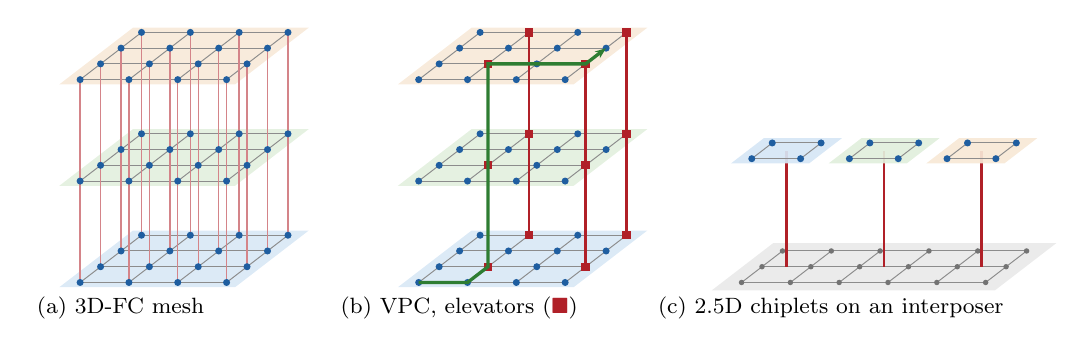
\begin{tikzpicture}[x={(0.62cm,0cm)},y={(0.26cm,0.20cm)},z={(0cm,0.92cm)},
  node/.style={circle,fill=acc2,inner sep=0.9pt},
  enode/.style={rectangle,fill=acc,inner sep=1.5pt},
  lnk/.style={draw=black!45,line width=0.35pt},
  vl/.style={draw=acc,line width=0.9pt}]
% ---------- (a) 3D-FC, 4x4x3
\begin{scope}
  \foreach \z/\c in {0/lay1,1/lay2,2/lay3} {
    \fill[\c,opacity=0.85] (-0.3,-0.3,\z*1.4) -- (3.3,-0.3,\z*1.4) -- (3.3,3.3,\z*1.4) -- (-0.3,3.3,\z*1.4) -- cycle;
    \foreach \x in {0,...,3} \foreach \y in {0,...,3} {
      \ifnum\x<3 \draw[lnk] (\x,\y,\z*1.4) -- (\x+1,\y,\z*1.4); \fi
      \ifnum\y<3 \draw[lnk] (\x,\y,\z*1.4) -- (\x,\y+1,\z*1.4); \fi
    }
  }
  \foreach \x in {0,...,3} \foreach \y in {0,...,3} {
    \draw[vl,draw=acc!55,line width=0.5pt] (\x,\y,0) -- (\x,\y,2.8);
    \foreach \z in {0,1,2} \node[node] at (\x,\y,\z*1.4) {};
  }
  \node[font=\footnotesize] at (1.5,-1.6,0) {(a) 3D-FC mesh};
\end{scope}
% ---------- (b) VPC with stride-2 elevators
\begin{scope}[xshift=4.3cm]
  \foreach \z/\c in {0/lay1,1/lay2,2/lay3} {
    \fill[\c,opacity=0.85] (-0.3,-0.3,\z*1.4) -- (3.3,-0.3,\z*1.4) -- (3.3,3.3,\z*1.4) -- (-0.3,3.3,\z*1.4) -- cycle;
    \foreach \x in {0,...,3} \foreach \y in {0,...,3} {
      \ifnum\x<3 \draw[lnk] (\x,\y,\z*1.4) -- (\x+1,\y,\z*1.4); \fi
      \ifnum\y<3 \draw[lnk] (\x,\y,\z*1.4) -- (\x,\y+1,\z*1.4); \fi
    }
  }
  \foreach \x/\y in {1/1,3/1,1/3,3/3} \draw[vl] (\x,\y,0) -- (\x,\y,2.8);
  \foreach \x in {0,...,3} \foreach \y in {0,...,3} \foreach \z in {0,1,2} \node[node] at (\x,\y,\z*1.4) {};
  \foreach \x/\y in {1/1,3/1,1/3,3/3} \foreach \z in {0,1,2} \node[enode] at (\x,\y,\z*1.4) {};
  % a route: source (0,0,0) -> elevator (1,1) -> up -> destination (3,2,2)
  \draw[c3,line width=1.2pt,-{Stealth[length=4pt]}] (0,0,0) -- (1,0,0) -- (1,1,0) -- (1,1,2.8) -- (2,1,2.8) -- (3,1,2.8) -- (3,2,2.8);
  \node[font=\footnotesize] at (1.5,-1.6,0) {(b) VPC, elevators (\textcolor{acc}{$\blacksquare$})};
\end{scope}
% ---------- (c) 2.5D
\begin{scope}[xshift=8.4cm]
  \fill[black!8] (-0.4,-0.5,0) -- (5.4,-0.5,0) -- (5.4,2.5,0) -- (-0.4,2.5,0) -- cycle;
  \foreach \x in {0,...,5} \foreach \y in {0,...,2} {
     \ifnum\x<5 \draw[lnk] (\x,\y,0) -- (\x+1,\y,0); \fi
     \ifnum\y<2 \draw[lnk] (\x,\y,0) -- (\x,\y+1,0); \fi
     \node[node,fill=black!55,inner sep=0.7pt] at (\x,\y,0) {};
  }
  \foreach \ox/\c in {0/lay1,2/lay2,4/lay3} {
    \draw[vl] (\ox+0.5,1,0) -- (\ox+0.5,1,1.6);
    \fill[\c,opacity=0.92] (\ox-0.3,0.2,1.6) -- (\ox+1.3,0.2,1.6) -- (\ox+1.3,1.8,1.6) -- (\ox-0.3,1.8,1.6) -- cycle;
    \foreach \i in {0,1} \foreach \j in {0,1} {
      \ifnum\i<1 \draw[lnk] (\ox+\i,0.5+\j,1.6) -- (\ox+\i+1,0.5+\j,1.6); \fi
      \ifnum\j<1 \draw[lnk] (\ox+\i,0.5+\j,1.6) -- (\ox+\i,1.5+\j,1.6); \fi
      \node[node] at (\ox+\i,0.5+\j,1.6) {};
    }
  }
  \node[font=\footnotesize] at (2.5,-1.6,0) {(c) 2.5D chiplets on an interposer};
\end{scope}
\end{tikzpicture}
\caption{Integration styles covered by the survey. (a) Fully connected 3D mesh: every router has vertical links. (b) Vertically partially connected stack with stride-2 elevators; the highlighted route reaches an elevator, climbs, and completes its planar path on the destination tier. (c) 2.5D system: chiplet networks connected through vertical links (VLs) to an interposer network.}
\label{fig:arch}
\end{figure}

\subsection{Router model and flow control}
\label{sec:bg-router}

We consider input-queued wormhole routers with $V$ virtual channels (VCs) per input port and credit-based flow control~\cite{dally2004principles}. A packet of $L$ flits is routed by its head flit: route computation returns a set of admissible (port, VC) pairs; the VC allocator grants one free output VC; the switch allocator then schedules flits through the crossbar, one per output per cycle. Two micro-architectural details matter for correctness and are rarely reported in the 3D routing literature.

\emph{VC reallocation.} An output VC is released when the tail flit of its owner leaves the router. Under \emph{atomic} reallocation it is granted to a new packet only once the downstream buffer is empty, so that a VC buffer never holds flits of two packets. Under \emph{non-atomic} reallocation it is granted as soon as the tail has left, and the head of the next packet queues behind the tail of the previous one in the downstream buffer. Non-atomic reuse improves buffer utilisation and is the default behaviour of a wormhole router with a single FIFO per input port; BookSim exposes the choice as \texttt{wait\_for\_tail\_credit}~\cite{jiang2013booksim}.

\emph{Arbitration.} Separable round-robin allocators are locally fair: each input competes on equal terms at each router. Locally fair arbitration is globally unfair in multi-hop networks: a flow that joins a congested path close to the bottleneck competes once and obtains half of the bandwidth at that merge, whereas a flow that has already crossed $k$ such merges obtains a share that decays geometrically with $k$ (the parking-lot effect)~\cite{dally2004principles}. Fairness therefore depends on the arbitration policy as well as on the routing algorithm; our evaluation varies only the latter (\cref{sec:rq-perf}).

\subsection{Routing relations, selection and adaptiveness}
\label{sec:bg-routing}

Let $\mathcal{N}$ be the set of routers and $\Ch$ the set of channels, a channel being a (link, VC) pair; injection and ejection channels are included.

\begin{definition}[Routing relation and selection]\label{def:routing}
A \emph{routing relation} is a map $\R:\Ch\times\mathcal{N}\to 2^{\Ch}$ that gives, for a head flit in input channel $c$ destined to $d$, the set of admissible output channels. A \emph{selection function} chooses one element of $\R(c,d)$ using network state. $\R$ is \emph{deterministic} if $|\R(c,d)|=1$ for all $(c,d)$, \emph{oblivious} if the choice among several admissible channels does not depend on network state, and \emph{adaptive} otherwise; it is \emph{minimal} if every admissible channel reduces the distance to $d$.
\end{definition}

This separation matters for evaluation: deadlock freedom is a property of $\R$ and of the router, whereas performance depends on the selection function. Most algorithms of the last five years are new selection functions on top of a small number of routing relations (\cref{sec:review}).

\begin{definition}[Degree of adaptiveness]\label{def:alpha}
For a minimal routing relation and a source--destination pair $(s,d)$ with absolute offsets $(\Delta_x,\Delta_y,\Delta_z)$ (numbers of hops per dimension), let $\Pmin(s,d)$ be the set of minimal paths, $|\Pmin(s,d)|=\binom{\Delta_x+\Delta_y+\Delta_z}{\Delta_x,\,\Delta_y,\,\Delta_z}$, and $\mathcal{P}_\R(s,d)\subseteq\Pmin(s,d)$ the paths that $\R$ admits. The degree of adaptiveness is $\alpha(s,d)=|\mathcal{P}_\R(s,d)|/|\Pmin(s,d)|$; we report its mean over ordered pairs together with the fraction of pairs for which $|\mathcal{P}_\R(s,d)|>1$.
\end{definition}

\subsection{Deadlock: theorems and their assumptions}
\label{sec:bg-deadlock}

\begin{definition}[Channel dependency graph]\label{def:cdg}
The channel dependency graph (CDG) of $\R$ is the directed graph $D=(\Ch,E)$ with $(c_i,c_j)\in E$ if and only if there is a destination $d$ such that a packet destined to $d$ can occupy $c_i$ and $c_j\in\R(c_i,d)$.
\end{definition}

\begin{theorem}[Dally and Seitz~\cite{dally1987deadlock}]\label{thm:dally}
A routing relation whose CDG is acyclic is deadlock-free. For a deterministic relation the condition is also necessary when every cycle of the CDG can be filled by packets, as for the dimension-order and turn-model relations considered here.
\end{theorem}

In general a cyclic CDG does not prove that a deadlock is reachable; the checker of \cref{sec:checker} therefore reports a cycle as a witness, to be confirmed by simulation or by a reachability argument.

Acyclicity can be obtained by forbidding turns (the turn model and its 3D variants such as negative-first, 4NP-first and odd--even~\cite{glass1992turn,chiu2000oddeven,pasricha2011lowoverhead}), by labelling nodes along a Hamiltonian path and allowing only label-monotone moves~\cite{lin1994hamiltonian,ebrahimi2013hamfa}, or by separating traffic into ordered virtual networks, which is how Elevator-First avoids cycles across tiers~\cite{dubois2013elevator}. Fully adaptive routing, whose CDG is cyclic, needs the weaker condition of Duato.

\begin{definition}[Escape subnetwork]\label{def:escape}
A routing subrelation $\R_1\subseteq\R$ on channels $\Ch_1\subseteq\Ch$ is an \emph{escape subnetwork} if it is connected (every destination is reachable from every channel through $\Ch_1$) and, from every state of $\R$, a blocked head flit may always request a channel of $\R_1$.
\end{definition}

\begin{theorem}[Duato~\cite{duato1993theory,duato1995necessary}]\label{thm:duato}
Under wormhole switching, a connected adaptive routing relation $\R$ is deadlock-free if it has an escape subnetwork $\R_1$ whose extended channel dependency graph is acyclic. The extended graph adds to the CDG of $\R_1$ the indirect dependencies created by packets that leave $\Ch_1$ and later re-enter it, and the cross dependencies created when channels of $\Ch_1$ are also used by packets that are not routed by $\R_1$.
\end{theorem}

In the common \emph{no-return} implementation the escape channels are VC~0 routed by dimension order and a packet that enters VC~0 stays there; the extended graph then reduces to the CDG of dimension-order routing, which is acyclic. Verbeek and Schmaltz gave necessary and sufficient conditions that tolerate richer routing relations~\cite{verbeek2011necessary}.

\paragraph{The hidden assumption.} \Cref{thm:duato} is proved for a switching model in which a queue does not accept the head of a new packet before it has emptied the previous one~\cite{duato1993theory}. This is atomic reallocation (\cref{sec:bg-router}). Ma et~al.\ observed that, with non-atomic allocation, ``a deadlock configuration is easily formed'' in fully adaptive routing and designed whole-packet forwarding to recover buffer utilisation without losing the guarantee~\cite{ma2012wpf}. The mechanism is simple and we state it because it explains a result of \cref{sec:rq-correct}.

\begin{proposition}[Commitment under non-atomic reallocation]\label{prop:nonatomic}
Consider a router that never revokes a VC grant, as in our simulator and in BookSim. With non-atomic reallocation, a head flit may be granted an adaptive output VC whose downstream buffer still holds flits of a previous packet. From that moment it waits for that VC alone and can no longer request the escape subnetwork. If the previous packet is itself committed to a non-empty adaptive VC, a cycle of such commitments is a deadlock that \cref{thm:duato} does not exclude.
\end{proposition}

\begin{proof}[Proof sketch]
The escape argument of \cref{thm:duato} requires that a blocked head can always fall back on an escape channel. A head that has already been allocated a VC has no allocation left to make; it only waits for credits of that VC. The waits-for relation among committed heads therefore follows dependencies between adaptive channels, which form cycles (\cref{tab:cdg}). A cycle in which every queue is full and every head is committed to the next queue is a legal, persistent state; \cref{fig:witness} shows one that our simulator reached.
\end{proof}

Livelock and starvation are distinct failures: minimal routing cannot livelock, non-minimal routing needs a bound on misrouting, and starvation is excluded only by starvation-free arbitration.

\subsection{Fault model}
\label{sec:bg-fault}

Planar links fail independently with probability $p_h$. Vertical faults follow a Gaussian copula: for each tier boundary $b$, a zero-mean Gaussian field $Z_b(x,y)$ over the $k_xk_y$ columns has covariance
\begin{equation}\label{eq:copula}
\operatorname{Cov}\bigl(Z_b(x,y),Z_b(x',y')\bigr)=\exp\!\bigl(-\lVert(x,y)-(x',y')\rVert_2/\xi\bigr),
\end{equation}
and the vertical segment of column $(x,y)$ across boundary $b$ fails if and only if $Z_b(x,y)<\Phi^{-1}(p_v)$. Every segment fails with probability exactly $p_v$, whatever the correlation length $\xi$; $\xi=0$, understood as the limit $\xi\to0$ in which distinct columns are uncorrelated, gives independent faults, and larger $\xi$ produces clusters of failed columns, consistent with the clustering reported for TSV defects~\cite{dang2021hotcluster,wang2015clustering}. Boundaries are mutually independent. Keeping the marginal fixed isolates the effect of correlation from that of the fault rate.

\subsection{Structural observability (ERA)}
\label{sec:bg-era}

Scalar averages compress a simulation into a few numbers. The Entropic Structural Observability framework~\cite{mesellem2026era}, abbreviated ERA here, analyses instead the trace of typed packet events (injection, forwarding, reception, drop) as probability distributions over resources: routers, directed links, time windows, buffers and, in 3D, TSV columns. For a distribution with Shannon entropy $H$ over $m_{\mathrm{act}}$ active among $m_{\mathrm{full}}$ resources it reports the normalised entropies $\hact{}=H/\log_2 m_{\mathrm{act}}$ and $\hfull{}=H/\log_2 m_{\mathrm{full}}$, the effective support $S_{\mathrm{eff}}=2^H$ and the concentration $1-\hact{}$. The router~$\times$~window activity matrix yields the space--time mutual information $I(R;W)$, its normalised effect size $\kappa_{ST}=I(R;W)/\min\{H(R),H(W)\}$ and a permutation $p$-value ($B=200$ permutations); the Jensen--Shannon divergence between consecutive windows measures drift; Jain's index and related indicators measure imbalance. ERA does not alter the simulation; it is a diagnostic layer on its trace. We use it as dimension \D{7} and to expose deadlock and hotspot signatures that scalar metrics miss (\cref{sec:rq-structure}).

% =====================================================================
\section{Survey methodology}
\label{sec:survey-method}

\paragraph{Scope.} We include peer-reviewed proposals of routing algorithms or selection policies for fully connected 3D meshes, vertically partially connected stacks, 2.5D chiplet networks and hybrid wired--wireless 3D networks published between January 2021 and October 2026, together with 2D proposals that report a 3D evaluation. We exclude task mapping, scheduling and thermal management that do not change routing decisions, purely wireless or optical interconnects, and routing proposals of the present authors. Historical designs published before 2021 are included as reference points when they define a routing relation still used as a baseline or as the deadlock argument of later work.

\paragraph{Identification.} Candidates were identified by keyword searches of publisher databases and scholarly indexes (IEEE Xplore, ACM Digital Library, SpringerLink, ScienceDirect, MDPI, dblp, OpenAlex, Crossref) with combinations of \emph{3D NoC}, \emph{3D network-on-chip}, \emph{partially connected}, \emph{elevator}, \emph{TSV}, \emph{chiplet}, \emph{interposer} with \emph{routing}, \emph{fault-tolerant}, \emph{thermal-aware}, \emph{deadlock}, \emph{reinforcement learning} and \emph{security}, followed by backward snowballing from recent surveys~\cite{touati2020survey,kaur2024mapping,muhsen2024review,biglari2024survey,ibarra2026learning,kondoth2026survey} and from the reference lists of included papers.

\paragraph{Verification standard.} Every attribute in \cref{tab:corpus,tab:hist} was read from the full text or, when the full text was not accessible to us, from the publisher record. An attribute that could not be verified from either is marked n/v rather than inferred from the abstract, the title or secondary citations. Bibliographic data were checked against the publisher or a DOI registry. One directly relevant survey, on routing algorithms and router microarchitectures of 3D NoCs (Journal of Systems Architecture, 2025; ScienceDirect PII S1383762125001018), was not accessible to us and its author list could not be verified; it is therefore not cited formally, and \cref{tab:surveys} does not position our work against it.

\paragraph{Limitations.} The corpus is curated, not exhaustive: we do not claim to have found every 3D routing paper of the period, and we report no screening counts that we could not reproduce. Its purpose is to support a critical review and a reproducible audit (\cref{sec:practice}); the evaluation of \cref{sec:protocol,sec:results} does not depend on the corpus being complete, because it evaluates the routing \emph{classes} on which the surveyed proposals are built (\cref{tab:classes}).

% =====================================================================
\section{Taxonomy and corpus}
\label{sec:taxonomy}

We classify proposals along four orthogonal axes (\cref{fig:taxonomy}). Axis~A is the \emph{integration style} (\cref{sec:bg-arch}). Axis~B is the \emph{mechanism} by which the proposal obtains adaptivity while preserving deadlock freedom: deterministic or oblivious routes; turn restrictions, including turn models designed by hand, by number-theoretic rules or by integer linear programming; node labelling (Hamiltonian, circular); escape channels in the sense of \cref{thm:duato}; ordered virtual networks, which is how most VPC and 2.5D schemes separate up-going from down-going traffic; reconfigurable tables; learned selection; and heuristic selection, including probabilistic beltways and game-theoretic schemes. Axis~C is the \emph{objective} (congestion, planar faults, vertical faults, thermal behaviour, energy, security). Axis~D is the \emph{information} used by the selection: local (own buffers and credits), regional (one- or two-hop neighbourhood, aggregated congestion as in RCA~\cite{gratz2008rca}), global (a network-wide view, online or computed offline), or learned (tables updated from experience). The axes are orthogonal in principle, and correlated in practice: VPC proposals favour virtual networks and elevator-level information, learning-based proposals target thermal and fault objectives, and 2.5D proposals concentrate on deadlock composition.

\begin{figure}[tbp]
\centering
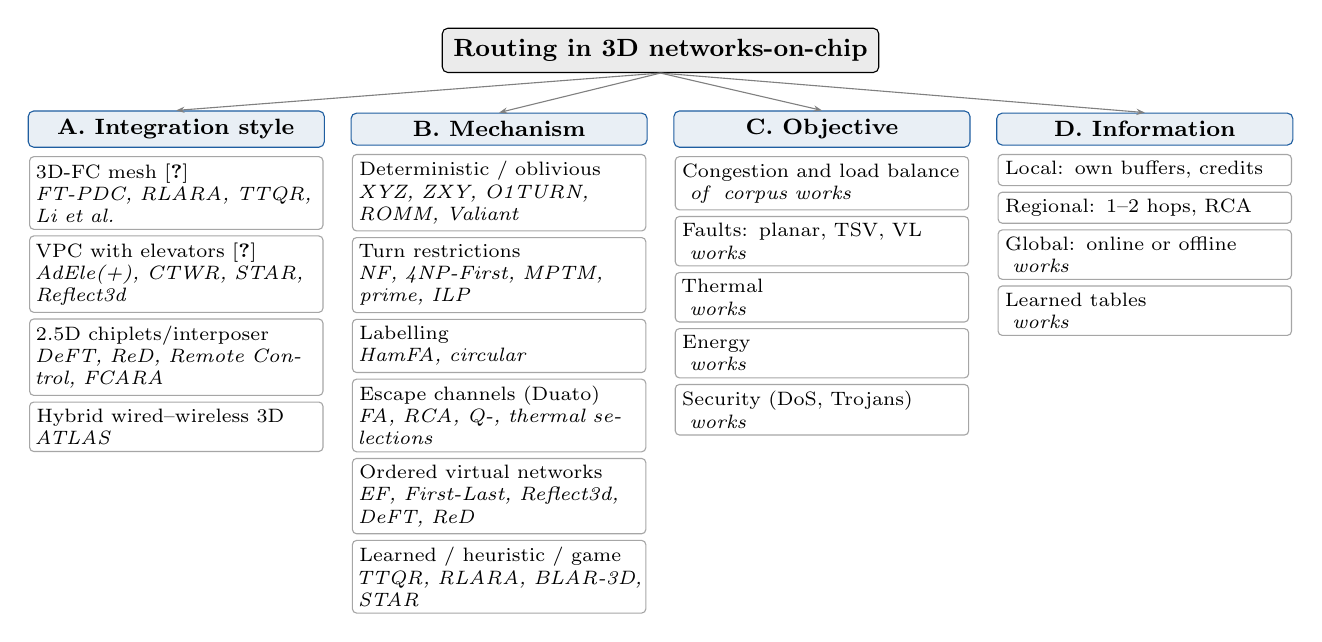
\begin{tikzpicture}[
  font=\scriptsize,
  root/.style={draw=black,fill=black!8,rounded corners=2pt,inner sep=4pt,font=\small\bfseries},
  axis/.style={draw=acc2,fill=acc2!10,rounded corners=2pt,text width=3.55cm,align=center,inner sep=3pt,font=\footnotesize\bfseries},
  leaf/.style={draw=black!35,fill=white,rounded corners=1.5pt,text width=3.55cm,align=left,inner sep=2.5pt},
  edge/.style={draw=black!50,-{Stealth[length=3pt]}}]
\node[root] (r) at (0,0) {Routing in 3D networks-on-chip};
\node[axis] (A) at (-6.15,-1.0) {A. Integration style};
\node[axis] (B) at (-2.05,-1.0) {B. Mechanism};
\node[axis] (C) at (2.05,-1.0) {C. Objective};
\node[axis] (D) at (6.15,-1.0) {D. Information};
\foreach \n in {A,B,C,D} \draw[edge] (r.south) -- (\n.north);
% axis A
\node[leaf,below=3pt of A] (A1) {3D-FC mesh~\cite{pavlidis2007topologies}\\ \textit{FT-PDC, RLARA, TTQR, Li et al.}};
\node[leaf,below=2pt of A1] (A2) {VPC with elevators~\cite{dubois2013elevator}\\ \textit{AdEle(+), CTWR, STAR, Reflect3d}};
\node[leaf,below=2pt of A2] (A3) {2.5D chiplets/interposer\\ \textit{DeFT, ReD, Remote Control, FCARA}};
\node[leaf,below=2pt of A3] (A4) {Hybrid wired--wireless 3D\\ \textit{ATLAS}};
% axis B
\node[leaf,below=3pt of B] (B1) {Deterministic / oblivious\\ \textit{XYZ, ZXY, O1TURN, ROMM, Valiant}};
\node[leaf,below=2pt of B1] (B2) {Turn restrictions\\ \textit{NF, 4NP-First, MPTM, prime, ILP}};
\node[leaf,below=2pt of B2] (B3) {Labelling\\ \textit{HamFA, circular}};
\node[leaf,below=2pt of B3] (B4) {Escape channels (Duato)\\ \textit{FA, RCA, Q-, thermal selections}};
\node[leaf,below=2pt of B4] (B5) {Ordered virtual networks\\ \textit{EF, First-Last, Reflect3d, DeFT, ReD}};
\node[leaf,below=2pt of B5] (B6) {Learned / heuristic / game\\ \textit{TTQR, RLARA, BLAR-3D, STAR}};
% axis C
\node[leaf,below=3pt of C] (C1) {Congestion and load balance\\ \textit{\val{corpus.obj.congestion} of \val{corpus.n} corpus works}};
\node[leaf,below=2pt of C1] (C2) {Faults: planar, TSV, VL\\ \textit{\val{corpus.obj.faults} works}};
\node[leaf,below=2pt of C2] (C3) {Thermal\\ \textit{\val{corpus.obj.thermal} works}};
\node[leaf,below=2pt of C3] (C4) {Energy\\ \textit{\val{corpus.obj.energy} works}};
\node[leaf,below=2pt of C4] (C5) {Security (DoS, Trojans)\\ \textit{\val{corpus.obj.security} works}};
% axis D
\node[leaf,below=3pt of D] (D1) {Local: own buffers, credits};
\node[leaf,below=2pt of D1] (D2) {Regional: 1--2 hops, RCA};
\node[leaf,below=2pt of D2] (D3) {Global: online or offline\\ \textit{\val{corpus.info.global} works}};
\node[leaf,below=2pt of D3] (D4) {Learned tables\\ \textit{\val{corpus.info.learned} works}};
\end{tikzpicture}
\caption{Four-axis taxonomy. Leaves list representative designs; counts refer to the \val{corpus.n}-work corpus of \cref{tab:corpus} (a work may pursue several objectives).}
\label{fig:taxonomy}
\end{figure}

\Cref{tab:corpus} lists the \val{corpus.n} works of the corpus and \cref{tab:hist} the \val{corpus.hist} historical reference designs. Three features of the corpus are worth stating before the review. First, the field is active and dispersed: \val{corpus.y2021}, \val{corpus.y2022}, \val{corpus.y2023}, \val{corpus.y2024}, \val{corpus.y2025} and \val{corpus.y2026} works appeared in 2021--2026 respectively, in venues ranging from DAC and IEEE Transactions on Computers to regional journals. Second, \val{corpus.vpc} works target VPC stacks and \val{corpus.25d} target 2.5D systems, so that more than a third of the recent effort concerns topologies in which vertical connectivity is scarce by design. Third, congestion is the most frequent objective (\val{corpus.obj.congestion} works); \val{corpus.obj.faults} works target faults and \val{corpus.obj.thermal} temperature, often together with congestion, and only \val{corpus.obj.security} target security.

\begin{table}[p]
\centering
\caption{Corpus of routing proposals for 3D, VPC and 2.5D NoCs, 2021--2026. DL, deadlock argument: F formal and inspectable (dependency graph, Duato, ordered virtual networks, turn-model proof); R inherited from a cited deadlock-free routing function; C claimed without an inspectable argument; I deadlock risk reduced or detected, not excluded; N not discussed; n/v not verifiable from an accessible record. Baselines: det.\ deterministic only; adapt.\ at least one adaptive or congestion-aware baseline.}
\label{tab:corpus}
\scriptsize
\setlength{\tabcolsep}{2.4pt}
\renewcommand{\arraystretch}{1.08}
\begin{tabularx}{\linewidth}{@{}>{\raggedright\arraybackslash}p{2.35cm}c>{\raggedright\arraybackslash}p{1.9cm}>{\raggedright\arraybackslash}p{1.35cm}>{\raggedright\arraybackslash}X>{\raggedright\arraybackslash}p{2.0cm}>{\raggedright\arraybackslash}p{1.3cm}c>{\raggedright\arraybackslash}p{1.45cm}c@{}}
\toprule
Algorithm & Year & Venue & Topology & Mechanism (axis B) & Objective (axis C) & Info.\\ (axis D) & DL & Simulator & Base. \\
\midrule
AdEle~\cite{taheri2021adele} & 2021 & DAC & VPC & offline elevator subsets + skip-RR & congestion, energy & local & R & Access Noxim & adapt. \\
Asymmetric edge routers~\cite{kunthara2021edge} & 2021 & Nano Commun. Netw. & 3D-FC & bufferless deflection, interleaved edge routers & congestion, energy & local & F & BookSim & adapt. \\
Reflect3d~\cite{silva2021reflect3d} & 2021 & SBCCI & VPC & 4 ordered VNs on 2 VCs, elevator search & faults, congestion & local & F & RTL (ModelSim) & adapt. \\
Remote Control~\cite{majumder2021remote} & 2021 & IEEE TC & 2.5D & boundary buffer reservation & deadlock avoidance & local & F & n/v & adapt. \\
DeFT~\cite{taheri2022deft} & 2022 & DATE & 2.5D & virtual networks + VL selection & VL faults, congestion & local & F & Noxim (ext.) & adapt. \\
Directional TA~\cite{kaleem2022directional} & 2022 & IJEECS & 3D-FC & directional minimal & thermal & local & n/v & n/v & n/v \\
FT-PDC~\cite{khodadadi2022ftpdc} & 2022 & J. Supercomput. & 3D-FC & path-diversity selection & faults, congestion & two-hop & n/v & n/v & n/v \\
LETHOR~\cite{safari2022lethor} & 2022 & J. Supercomput. & 3D-FC & proactive avoidance of hot regions & thermal & layer-wide & n/v & n/v & n/v \\
STTAR~\cite{fang2022sttar} & 2022 & CMC & 3D-FC & score-based + buffer resizing & thermal, congestion & local & n/v & n/v & n/v \\
TTQR~\cite{liu2022ttqr} & 2022 & Sensors & 3D-FC & two Q-tables (traffic, thermal) & thermal, congestion & learned & n/v & Access Noxim & adapt. \\
AdEle+~\cite{taheri2023adeleplus} & 2023 & IEEE TC & VPC & offline subsets + skip-RR & congestion, energy & local & R & Access Noxim & adapt. \\
Gaffour et al.~\cite{gaffour2023congestion} & 2023 & IJCA & 2D/3D & congestion-aware selection & congestion & local & n/v & n/v & n/v \\
Li et al.~\cite{jiao2023aftc} & 2023 & Microelectron. J. & 3D-FC & diagonal regions & faults, congestion & local & n/v & n/v & n/v \\
Prime turn model~\cite{sharma2023prime} & 2023 & CCIS & 3D-FC & prime-number turn rules, no VC & congestion & local & C & n/v & n/v \\
RLARA~\cite{jiao2023rlara} & 2023 & Electronics & 3D-FC & TSV-aware Q-table (k-means) & TSV faults & learned & I & Garnet 2.0 & n/v \\
ILP turn design~\cite{liu2024ilp} & 2024 & SOCC & 2.5D & ILP-optimal turn restrictions & deadlock, load, faults & offline & F & n/v & n/v \\
ReD~\cite{taheri2024red} & 2024 & IEEE TCAD & 2.5D & two VNs with distinct turn models & HL and VL faults & local & F & n/v & n/v \\
SCRIPT~\cite{taheri2024script} & 2024 & GLSVLSI & 2.5D & multi-objective path concealment & security (DDoS) & global (offline) & n/v & n/v & n/v \\
AMBTAR~\cite{dadmand2025ambtar} & 2025 & J. Supercomput. & 3D-FC & probabilistic beltways (non-minimal) & thermal & n/v & n/v & n/v & n/v \\
CTWR~\cite{ctwr2025} & 2025 & Comput. Electr. Eng. & VPC & multi-criteria inter-layer & congestion, thermal, wear & local + global & n/v & Access Noxim & n/v \\
FCARA~\cite{zhou2025fcara} & 2025 & J. Electron. Inf. Technol. & 2.5D & joint fault--congestion cost & faults, congestion & local & C & Chiplet\-Simulator & adapt. \\
Passage-based~\cite{kurokawa2025passage} & 2025 & Chips & 3D-FC & passage-based detours & faults & local & n/v & n/v & n/v \\
Securet3d~\cite{dasilva2025securet3d} & 2025 & IEEE TVLSI & VPC & secure path establishment & security, faults & n/v & n/v & n/v & n/v \\
ATLAS~\cite{singh2026atlas} & 2026 & JETTA & 3D + wireless & hierarchical planning + local adaptation & faults, congestion, thermal & global + local & n/v & Access Noxim & det. \\
BLAR-3D~\cite{aslan2026blar} & 2026 & DDECS & 3D-FC & Q-learning + beta selection & congestion & learned & n/v & n/v & n/v \\
STAR~\cite{ning2026star} & 2026 & J. Supercomput. & VPC & Stackelberg game & thermal, delay & global & n/v & Noxim & n/v \\
\bottomrule
\end{tabularx}
\end{table}

\begin{table}[tbp]
\centering
\caption{Historical reference designs (before 2021) used as baselines or as deadlock arguments by the corpus. Deadlock argument as in \cref{tab:corpus}.}
\label{tab:hist}
\scriptsize
\setlength{\tabcolsep}{3pt}
\begin{tabularx}{\linewidth}{@{}>{\raggedright\arraybackslash}p{3.6cm}c>{\raggedright\arraybackslash}p{2.0cm}>{\raggedright\arraybackslash}X c@{}}
\toprule
Design & Year & Topology & Mechanism & Deadlock argument \\
\midrule
Planar-adaptive~\cite{chien1995planar} & 1995 & $k$-ary $n$-mesh & adaptive in successive planes, 3 VCs & F \\
RILM~\cite{rusu2010rilm} & 2010 & 3D & reconfigurable inter-layer routing & n/v \\
4NP-First / Pasricha--Zou~\cite{pasricha2011lowoverhead} & 2011 & 3D-FC & turn-model fault tolerance & F \\
AFRA~\cite{akbari2012afra} & 2012 & 3D-FC & ZXY with XZXY detours & F \\
Elevator-First~\cite{dubois2013elevator} & 2013 & VPC & nearest elevator, up/down virtual networks & F \\
HamFA~\cite{ebrahimi2013hamfa} & 2013 & 3D-FC & Hamiltonian path, no VC & F \\
Circular~\cite{alizadeh2014circular} & 2014 & 3D-FC & circular labelling, no VC & F \\
FT-DyXYZ~\cite{jouybari2014dyxyz} & 2014 & 3D-FC & proximity congestion & n/v \\
HARS~\cite{zhou2014hars} & 2014 & 3D-FC & reliable adaptive & n/v \\
REDELF~\cite{lee2015redelf} & 2015 & VPC & energy-efficient elevator routing & n/v \\
LOFT~\cite{zhou2016loft} & 2016 & 3D-FC & tables + odd-even & n/v \\
Resilient PC-3D~\cite{salamat2016resilient} & 2016 & VPC & fault-resilient elevator routing & n/v \\
First-Last~\cite{charif2018firstlast} & 2018 & VPC & positive-first/last virtual networks & F \\
LEAD~\cite{salamat2018lead} & 2018 & 3D & adaptive, queueing-verified & n/v \\
Modular routing~\cite{yin2018modular} & 2018 & 2.5D & modular turn restrictions & F \\
PDA-HyPAR~\cite{dai2018pdahypar} & 2018 & 3D-FC & hybrid planar adaptive & n/v \\
3DEP~\cite{vahdatpanah2019threedep} & 2019 & 3D-FC & even traffic distribution & n/v \\
CDA~\cite{fu2019cda} & 2019 & VPC & global buffer-aware elevators & n/v \\
ADFT~\cite{mogharrabi2020adft} & 2020 & 3D-FC & adaptive distributed FT & n/v \\
MPTM~\cite{cai2020mptm} & 2020 & 3D-FC & minimum-pressure turn model, no VC & F \\
Q-function TA~\cite{lee2020qthermal} & 2020 & 3D-FC & Q-learning over safe set & R \\
\bottomrule
\end{tabularx}
\end{table}

% =====================================================================
\section{Critical review}
\label{sec:review}

We review the field family by family. For each family we state the mechanism, the evidence offered for it, and what our common evaluation (\cref{sec:results}) adds. Forward references point to the dimension (\D{1}--\D{12}) that tests each claim.

\subsection{Deterministic and oblivious routing}
\label{sec:rev-det}

Dimension-order routing is the baseline of almost every paper in the corpus, almost always in the XYZ order. Its virtues are well known: an acyclic CDG with a single VC (\cref{thm:dally}), in-order delivery when a flow is confined to one VC (\cref{tab:reorder}), and logic small enough to be negligible (\D{8}). Its weaknesses are equally known: no path diversity and therefore no tolerance of a single faulty link on the route, and worst-case throughput on adversarial permutations that can be a small fraction of uniform throughput. Oblivious routing randomises the route without looking at the network: O1TURN chooses between two dimension orders per packet and reaches near-optimal worst-case throughput in 2D meshes with two VCs~\cite{seo2005o1turn}; ROMM chooses a random intermediate node inside the minimal box~\cite{nesson1995romm}; Valiant's scheme chooses it anywhere, trading twice the average distance for load balance on any permutation~\cite{valiant1981universal}.

Two observations recur in our evaluation. First, the dimension \emph{order} matters as much as determinism. Routing vertically first (ZXY), as AFRA does in its fault-free mode~\cite{akbari2012afra}, spreads vertical traffic over all columns and breaks the alignment that makes XYZ collapse on bit-reversal and similar patterns; ZXY is the only fully connected class that passes our traffic-robustness criterion (\D{4}, \cref{sec:rq-perf}). Second, comparing a new adaptive algorithm with XYZ only is a weak test: XYZ is close to the best possible class on uniform traffic and among the worst on bit-reversal-like permutations, so the outcome of the comparison is determined by the choice of traffic.

\subsection{Turn restrictions and labelling}
\label{sec:rev-turn}

Turn-model routing obtains adaptiveness without VCs by forbidding enough turns to break every cycle of the CDG~\cite{glass1992turn}. In 3D, negative-first, 4NP-First~\cite{pasricha2011lowoverhead} and the odd--even family~\cite{chiu2000oddeven} restrict different turn sets; MPTM uses a repetitive-turn concept to raise adaptiveness without VCs~\cite{cai2020mptm}; the prime-number turn model of Sharma et~al.\ restricts turns according to number-theoretic properties of node coordinates~\cite{sharma2023prime}; and Liu and Radetzki compute optimal turn restrictions for chiplet systems by integer linear programming~\cite{liu2024ilp}. Labelling schemes order the nodes along a Hamiltonian path (HamFA~\cite{ebrahimi2013hamfa}, after Lin et~al.~\cite{lin1994hamiltonian}) or along circular paths~\cite{alizadeh2014circular}; label-monotone moves are deadlock-free, and the two sub-networks of increasing and decreasing labels may use non-minimal moves around faults.

The weakness of the family is the asymmetry of its adaptiveness. Negative-first routing is fully adaptive for some quadrants of the offset space and deterministic for others; the 3D variant admits more than one path for \val{d2.nf.multi}\% of ordered pairs but only a fraction $\alpha=\val{d2.nf.alpha}$ of the minimal paths on average (\D{2}). This asymmetry turns into hot spots under load: in our sweeps the negative-first class saturates at \val{d3.sat.nf.random} flits/node/cycle on uniform traffic against \val{d3.sat.xyz.random} for XYZ (\D{3}). The Hamiltonian class admits many paths (\val{d2.ham.median} paths for the median pair) but concentrates traffic along the snake, and saturates at \val{d3.sat.ham.random}. Claims of turn-model papers are usually supported by a proof of deadlock freedom, which is the strength of the family; the prime turn model is an exception, since it claims deadlock freedom without an argument that a reader can check (\cref{tab:corpus}).

\subsection{Escape-channel adaptive routing and selection functions}
\label{sec:rev-escape}

Most adaptive proposals for 3D-FC meshes keep a minimal fully adaptive routing relation and protect it with an escape subnetwork (\cref{thm:duato}); their contribution is the \emph{selection function}. RCA aggregates congestion along each dimension~\cite{gratz2008rca}; DyAD switches between deterministic and adaptive modes~\cite{hu2004dyad}; FT-PDC selects by path diversity using two-hop information~\cite{khodadadi2022ftpdc}; 3DEP aims at an even distribution of traffic~\cite{vahdatpanah2019threedep}; Gaffour et~al.\ compare a congestion-aware selection in 2D and 3D~\cite{gaffour2023congestion}; Li et~al.\ define diagonal regions to co-optimise fault tolerance and congestion~\cite{jiao2023aftc}; PDA-HyPAR combines planar-adaptive routing~\cite{chien1995planar} with path-diversity awareness~\cite{dai2018pdahypar}; LEAD verifies its adaptive routing with a queueing model~\cite{salamat2018lead}.

The family deserves two criticisms. The first concerns correctness. The guarantee of \cref{thm:duato} holds for atomic VC reallocation; a paper that relies on it must therefore state which reallocation its router uses, which we found difficult to establish from the records we read, several of which are evaluated on simulators whose router is not described in the paper. \Cref{prop:nonatomic} shows that the guarantee is lost under non-atomic reuse, and our simulator turns this into an observation: every escape-based class deadlocked in at least half of its overload runs under non-atomic reallocation (\D{1}, \cref{sec:rq-correct}). The second concerns the evidence for the selection functions themselves. Under a paired design with common random numbers, regional congestion awareness, Q-routing and thermal-aware selection are within one percent of the simplest selection (largest number of free credits) on non-hotspot traffic (\cref{tab:stats}), and on hotspot traffic all of them, like the simplest selection, are more than four times slower than XYZ (\cref{tab:d4fc}); what they add is area, storage and side-band wiring (\D{8}). A gain over XYZ therefore says little about a selection function: the baseline it must beat is a well-implemented credit-based minimal adaptive selection with the same VCs and buffers.

\subsection{Elevator routing in partially connected stacks}
\label{sec:rev-vpc}

Elevator-First routes every inter-tier packet to an elevator, through two virtual networks for up-going and down-going traffic that keep the CDG acyclic~\cite{dubois2013elevator}. Later work refines the elevator choice and the planar sub-routes. REDELF targets energy efficiency~\cite{lee2015redelf}; the resilient scheme of Salamat et~al.\ adds a formal reliability analysis for VPC stacks~\cite{salamat2016resilient}; First-Last uses positive-first and positive-last virtual networks to obtain adaptiveness with two VCs~\cite{charif2018firstlast}; CDA assigns elevators dynamically using buffer information collected from the whole network~\cite{fu2019cda}; AdEle and AdEle+ precompute for each node a subset of candidate elevators offline and choose online among them with a congestion- and energy-aware skip policy~\cite{taheri2021adele,taheri2023adeleplus}; Reflect3d embeds four ordered virtual networks on two VCs to search for a healthy elevator~\cite{silva2021reflect3d}; CTWR combines congestion, temperature and wear into an inter-layer decision~\cite{ctwr2025}; Securet3d adds secure path establishment~\cite{dasilva2025securet3d}; STAR formulates inter-layer routing as a Stackelberg game over thermal, delay and throughput objectives~\cite{ning2026star}.

Deadlock freedom is comparatively well argued in this family: of the three members whose argument we could inspect, AdEle and AdEle+ inherit the virtual-network argument of Elevator-First explicitly and Reflect3d gives its own formal argument. It is also the family in which the evaluation is most sensitive to the elevator selection: in our runs, a global-load selection reduces latency by a median of \val{st.aesg.ef.nonhotspot.medabs}\% with respect to nearest-elevator selection and is the only VPC class that passes the traffic-robustness criterion (\D{4}), whereas the subset-based local selection of AdEle passes neither \D{4} nor \D{5} in our configuration. The global information that makes elevator selection effective must, however, be collected and distributed by hardware that none of the global schemes costs in its evaluation (\D{8}). And static elevator assignment loses every packet whose assigned elevator has failed---on average up to a fraction \val{d5.vpc.ef.maxdrop} of all injected packets per fault configuration in our runs, and up to \val{d5.vpc.ef.runmax} in a single run (\D{5}).

\subsection{Fault-tolerant routing}
\label{sec:rev-fault}

Fault tolerance in 3D NoCs ranges from reconfigurable inter-layer routing (RILM~\cite{rusu2010rilm}) and turn-model schemes (4NP-First~\cite{pasricha2011lowoverhead}) to detours around faulty vertical links (AFRA's XZXY detours~\cite{akbari2012afra}), table-based schemes combined with odd--even routing (LOFT~\cite{zhou2016loft}), congestion-aware proximity routing (FT-DyXYZ~\cite{jouybari2014dyxyz}), reliable adaptive routing (HARS~\cite{zhou2014hars}), distributed adaptive schemes (ADFT~\cite{mogharrabi2020adft}) and, in the corpus, passage-based detours~\cite{kurokawa2025passage}, diagonal regions~\cite{jiao2023aftc}, TSV-aware reinforcement learning~\cite{jiao2023rlara} and hierarchical planning with local adaptation over wired and wireless links~\cite{singh2026atlas}. On 2.5D systems, DeFT and ReD tolerate faulty vertical links between chiplets and interposer while keeping deadlock freedom with virtual networks~\cite{taheri2022deft,taheri2024red}, and FCARA adds a joint fault--congestion cost~\cite{zhou2025fcara}. Outside 3D, recent work combines fault tolerance with quality-of-service priorities~\cite{yu2025topsis}.

Three gaps stand out. First, fault models are independent and identically distributed almost everywhere, although TSV defects are known to cluster~\cite{dang2021hotcluster,wang2015clustering}; we did not find an inspectable record of the corpus that injects spatially correlated vertical faults. \Cref{sec:analytical} shows that correlation does not change the expected reachability of a static route but penalises local adaptive policies and raises the probability that a whole tier boundary is severed---by a factor of five or more with four elevators per boundary and by many orders of magnitude for dense layouts---which no routing algorithm can survive. Second, fault-tolerance claims are rarely separated from what any algorithm could achieve: we compare every policy with the connectivity bound of the faulty graph (\D{5}). Third, reconfiguration and learning-based schemes keep deadlock freedom by construction only if the reconfigured relation is checked; RLARA, for instance, reduces deadlock risk without excluding it (\cref{tab:corpus}).

\subsection{Thermal-aware routing}
\label{sec:rev-thermal}

Thermal-aware schemes steer traffic away from hot regions, either reactively from temperature sensors or proactively from predicted heat: the Q-function scheme of Lee and Han restricts learned choices to a safe set~\cite{lee2020qthermal}; STTAR scores candidate ports and resizes buffers~\cite{fang2022sttar}; directional schemes restrict the direction of minimal moves~\cite{kaleem2022directional}; LETHOR limits entrances to hot regions~\cite{safari2022lethor}; TTQR keeps separate Q-tables for traffic and temperature~\cite{liu2022ttqr}; AMBTAR uses probabilistic non-minimal beltways~\cite{dadmand2025ambtar}; STAR and CTWR include temperature in elevator selection~\cite{ning2026star,ctwr2025}. Thermal management of 3D systems more broadly relies on compact models such as 3D-ICE~\cite{sridhar2010ice} and combines routing with task migration and dynamic voltage and frequency scaling~\cite{huang2024dtm,tang2025migration,chen2023mlthermal}.

The critical question is leverage: how much can routing alone change temperature? In a 3D stack the dominant heat sources are the cores, and the network's share of power is a fraction of the total. Our compact model (\cref{sec:analytical}) shows that minimal routing changes the peak temperature by at most a few tenths of a kelvin relative to XYZ, that thermal-aware selection lowers it by \val{d10.ta.bestabs}\,K in the most favourable of our eight scenarios and by only \val{d10.ta.worstabs}\,K in the least favourable, and that non-minimal routing raises it by up to \val{d10.val.worstabs}\,K (\D{10}). Proposals reporting larger thermal benefits should state the network's share of power and the thermal parameters that produce them.

\subsection{Learning-based routing}
\label{sec:rev-learning}

Q-routing~\cite{boyan1994qrouting} estimates delivery times per destination and output port and updates them from neighbours' estimates. Its 3D descendants add thermal objectives (TTQR~\cite{liu2022ttqr}), TSV awareness with clustering (RLARA~\cite{jiao2023rlara}) or regulated exploration (BLAR-3D~\cite{aslan2026blar}); deep reinforcement learning frameworks such as DRLAR target 2D NoCs~\cite{wang2024drlar}. A recent scoping review of 48 studies of learning-based NoC routing reports missing deadlock guarantees and finds that only 37.5\% report synthesis results~\cite{ibarra2026learning}; see also the roadmap of Balamurugan et~al.~\cite{balamurugan2022roadmap}.

Our evaluation sharpens this diagnosis in two ways. A tabular Q-router for a 256-node mesh stores one estimate per destination and output port: \val{hw.qtable.bits} bits per router at 16 bits per entry, \val{hw.qtable.ratio} times the area of the whole two-VC baseline router in flip-flops (\D{8}). And once the Q-selection is placed on an escape-protected minimal relation---the only way we found to make it deadlock-free---it is practically equivalent to the simplest credit-based selection: the median paired difference is \val{st.qr.fa.nonhotspot.medabs}\%, although the small difference is statistically detectable (Holm $p$ = \val{st.qr.fa.nonhotspot.p}, \cref{tab:stats}). Learning can be justified in 3D NoCs, but only against a strong adaptive baseline and with its storage, update traffic and deadlock argument costed.

\subsection{Security-aware routing}
\label{sec:rev-security}

NoC security work catalogues eavesdropping, spoofing, denial-of-service (DoS) and hardware-Trojan threats~\cite{charles2021security,weerasena2023security}. Routing-level countermeasures in the corpus conceal paths against distributed DoS in chiplet systems (SCRIPT~\cite{taheri2024script}) or establish secure paths in VPC stacks (Securet3d~\cite{dasilva2025securet3d}); Rajan et~al.\ mitigate time-delay Trojans with a secure routing framework~\cite{rajan2023trojan}. An under-studied question is whether adaptivity itself changes the exposure to flooding. Our DoS experiment (\D{11}) gives a first answer: under eight flooding sources aimed at one node, and at the lower of our two benign loads, minimal adaptive routing inflates the latency of delivered benign packets \val{d11.fa.over.xyz} times more than XYZ, negative-first \val{d11.nf.over.xyz} times more, whereas the inflation of O1TURN is only \val{d11.o1t.over.xyz} times that of XYZ (\cref{sec:rq-cost} also reports the benign packets left undelivered). A plausible explanation is that adaptive routing spreads the attacker's congestion over more paths and so exposes more benign flows to it.

\subsection{2.5D, deflection and wireless schemes}
\label{sec:rev-25d}

Chiplet systems raise a composition problem: each chiplet may be internally deadlock-free while the system is not. Modular routing restricts turns at chiplet boundaries~\cite{yin2018modular}; Remote Control reserves boundary buffers to avoid deadlock~\cite{majumder2021remote}; DeFT and ReD use virtual networks with distinct turn models~\cite{taheri2022deft,taheri2024red}; the ILP design of Liu and Radetzki optimises the restrictions~\cite{liu2024ilp}. These works are, as a group, the most careful of the corpus about deadlock. Bufferless deflection routing, evaluated in 3D with interleaved asymmetric edge routers by Kunthara et~al.~\cite{kunthara2021edge}, avoids deadlock by construction but must bound livelock. Hybrid wired--wireless schemes such as ATLAS~\cite{singh2026atlas} add wireless links whose arbitration and failure modes are rarely modelled in routing evaluations. Our evaluation does not cover 2.5D, deflection or wireless designs; their routing relations depend on interposer topologies and wireless media that would require models of their own (\cref{sec:threats}).

% =====================================================================
\section{Audit of evaluation practice}
\label{sec:practice}

\Cref{tab:audit} summarises how the corpus supports its claims. We report counts over the records in which an attribute could be verified, and the number of unverifiable records separately.

\begin{table}[tbp]
\centering
\caption{Audit of the \val{corpus.n}-work corpus. Counts are over the records in which the attribute could be verified; every count except the last row is computed from the coded attributes of the artefact.}
\label{tab:audit}
\small
\begin{tabular}{@{}lrl@{}}
\toprule
Attribute & Count & Comment \\
\midrule
Deadlock argument verifiable & \val{corpus.dl.verif} & \val{corpus.dl.nv} records not verifiable \\
\quad formal and inspectable (F) & \val{corpus.formal} & mostly VPC and 2.5D schemes \\
\quad inherited from a cited function (R) & \val{corpus.inherit} & AdEle, AdEle+ (Elevator-First) \\
\quad claimed, mitigated or absent (C, I, N) & \val{corpus.weak} & Prime turn model, RLARA, FCARA \\
\addlinespace
Simulator identifiable & \val{corpus.sim.verif} & \val{corpus.simfamilies} simulator families (\val{corpus.simdistinct} tools) \\
\quad Noxim and derivatives & \val{corpus.noxim} & router micro-architecture rarely stated \\
\addlinespace
Baselines verifiable & \val{corpus.base.verif} & \\
\quad deterministic baselines only & \val{corpus.detonly} & XYZ-only comparisons \\
\quad at least one adaptive baseline & \val{corpus.adapt} & \\
\addlinespace
Correlated vertical faults injected & 0 & none found in the records we read (not coded) \\
\bottomrule
\end{tabular}
\end{table}

Four findings follow. (i) Of the \val{corpus.dl.verif} records whose deadlock argument we could inspect, \val{corpus.formal} give a formal argument, \val{corpus.inherit} inherit one, and \val{corpus.weak} claim deadlock freedom without an argument, merely reduce the risk, or do not discuss it. (ii) The \val{corpus.sim.verif} identifiable evaluations use \val{corpus.simfamilies} different simulator families (\val{corpus.simdistinct} tools if the Noxim variants are counted separately), \val{corpus.noxim} of them Noxim~\cite{catania2015noxim} or a derivative, with router models that differ in pipeline depth, buffering and allocation; results are therefore not comparable across papers. Because the correctness of escape-based designs depends on the VC reallocation policy (\cref{prop:nonatomic}), that policy should be stated; we found it difficult to locate in the records we read. (iii) Of the \val{corpus.base.verif} records whose baselines we could verify, \val{corpus.detonly} compares with deterministic baselines only; the others include at least one adaptive or congestion-aware baseline. (iv) We found no record whose fault model includes the spatial correlation of TSV defects.

These findings motivate the minimum reporting standard of \cref{tab:checklist}. None of its items is new in isolation; what is missing is their systematic application. Each item corresponds to one or more dimensions of our protocol, which shows that they are affordable.

\begin{table}[tbp]
\centering
\caption{Minimum reporting standard proposed for 3D NoC routing papers, with the protocol dimension that implements each item in this article.}
\label{tab:checklist}
\small
\begin{tabularx}{\linewidth}{@{}rX>{\raggedright\arraybackslash}p{2.0cm}@{}}
\toprule
\# & Item & This article \\
\midrule
1 & Deadlock-freedom argument for the routing relation \emph{and} the router: VC reallocation policy, escape usage, virtual-network ordering; ideally a mechanised check & \D{1}, \cref{sec:checker} \\
2 & Baselines: one deterministic, one oblivious and one well-implemented minimal adaptive routing with the same VCs and buffers & \val{cls.n} classes \\
3 & Traffic: uniform, at least two adversarial permutations, hotspot, bursty traffic, and a flooding scenario & \D{3}, \D{4}, \D{11} \\
4 & Full latency--load curves up to saturation with an explicit saturation criterion; overload behaviour & \D{3} \\
5 & At least five seeds per point, confidence intervals, paired tests with multiplicity correction & \cref{sec:stats} \\
6 & Fault model with stated marginals and spatial correlation; comparison with the connectivity bound & \D{5} \\
7 & Synthesised area of route and selection logic and of all added storage and wiring, including reorder buffers when packets of a flow can overtake each other & \D{8}, \cref{tab:reorder} \\
8 & Energy and thermal models with all parameters, and their sensitivity & \D{9}, \D{10} \\
9 & Sensitivity of conclusions to router parameters and network size & \D{12} \\
10 & Release of simulator, configurations, raw results and analysis scripts & artefact \\
\bottomrule
\end{tabularx}
\end{table}

% =====================================================================
\section{Evaluation protocol, platform and analytical models}
\label{sec:protocol}

\subsection{Routing classes}
\label{sec:classes}

Re-implementing every published algorithm is neither possible---most descriptions are not complete enough---nor necessary: as \cref{sec:review} showed, the corpus is built on a small number of routing relations combined with a larger number of selection functions. We therefore evaluate \val{cls.n} \emph{routing classes}, \val{cls.nfc} for 3D-FC meshes and \val{cls.nvpc} for VPC stacks, each an exact routing relation with an exact selection function (\cref{tab:classes}). A class represents the surveyed algorithms that share its relation and its kind of selection; where a surveyed algorithm adds features that we do not model (buffer resizing, wireless links, game-theoretic negotiation), we say so in \cref{sec:threats}. All classes share the same router, buffers, VC count (where the class needs fewer VCs than are available, it uses all of them as one class) and random-number streams.

\begin{table}[tbp]
\centering
\caption{Evaluated routing classes. VCs: minimum number of virtual channels required. Info: information used by the selection. Escape-based classes use VC~0 with XYZ routing as escape subnetwork (no return) and VC~1 as adaptive channel.}
\label{tab:classes}
\scriptsize
\setlength{\tabcolsep}{2.6pt}
\begin{tabularx}{\linewidth}{@{}l>{\raggedright\arraybackslash}p{4.1cm}>{\raggedright\arraybackslash}X c>{\raggedright\arraybackslash}p{1.35cm}>{\raggedright\arraybackslash}p{2.9cm}@{}}
\toprule
Class & Routing relation & Selection function & VCs & Info & Represents \\
\midrule
\cls{XYZ} & dimension order X, Y, Z & -- & 1 & -- & baseline of the corpus \\
\cls{ZXY} & dimension order Z, X, Y (vertical first) & -- & 1 & -- & AFRA, fault-free mode~\cite{akbari2012afra} \\
\cls{NF} & 3D negative-first turn model & largest number of free credits & 1 & local & turn models~\cite{glass1992turn,pasricha2011lowoverhead,cai2020mptm,sharma2023prime} \\
\cls{DyAD} & 3D negative-first & deterministic while the preferred port keeps $\ge25\%$ free credits, adaptive otherwise & 1 & local & DyAD~\cite{hu2004dyad} \\
\cls{HAM} & Hamiltonian snake labelling, label-monotone moves (may be non-minimal) & minimal moves first, then smallest label gap; credits & 1 & local & HamFA~\cite{ebrahimi2013hamfa}, circular~\cite{alizadeh2014circular} \\
\cls{O1T} & XYZ on VC class 0 or ZYX on class 1 & order drawn at injection & 2 & -- & O1TURN~\cite{seo2005o1turn} \\
\cls{ROMM} & two-phase XYZ through a random node of the minimal box & oblivious & 2 & -- & ROMM~\cite{nesson1995romm} \\
\cls{VAL} & two-phase XYZ through a random node & oblivious & 2 & -- & Valiant~\cite{valiant1981universal} \\
\cls{FA} & minimal fully adaptive + escape & largest number of free credits & 2 & local & escape-based designs~\cite{khodadadi2022ftpdc,vahdatpanah2019threedep,gaffour2023congestion,jiao2023aftc} \\
\cls{RCA} & as \cls{FA} & RCA-1D aggregated congestion, weight 0.5 & 2 & regional & RCA~\cite{gratz2008rca}, two-hop schemes \\
\cls{QR} & as \cls{FA} & Q-routing estimates, learning rate 0.5 & 2 & learned & Q-routing~\cite{boyan1994qrouting}, TTQR, RLARA, BLAR-3D \\
\cls{TA} & as \cls{FA} & coolest neighbour; temperatures from the compact model every 1000 cycles & 2 & sensors & STTAR, LETHOR, directional TA~\cite{fang2022sttar,safari2022lethor,kaleem2022directional} \\
\midrule
\cls{EF} & Elevator-First: up and down virtual networks; same-tier packets keep their VN & nearest elevator & 2 & -- & Elevator-First~\cite{dubois2013elevator}, REDELF~\cite{lee2015redelf} \\
\cls{EF-R} & as \cls{EF} & nearest healthy elevator & 2 & fault map & resilient elevator routing~\cite{salamat2016resilient,silva2021reflect3d} \\
\cls{AES-G} & as \cls{EF} & distance $+\,0.5\times$ elevator load (global) & 2 & global & CDA~\cite{fu2019cda}, CTWR, STAR \\
\cls{AdEle} & as \cls{EF} & 4 nearest elevators; skip-based round robin on EWMA costs ($a=0.2$, $\xi_s=0.05$, threshold 0.1) & 2 & local feedback & AdEle, AdEle+~\cite{taheri2021adele,taheri2023adeleplus} \\
\cls{FL} & First-Last: positive-first and positive-last VNs, strict VC separation & largest number of free credits within the VN & 2 & local & First-Last~\cite{charif2018firstlast} \\
\bottomrule
\end{tabularx}
\end{table}

\subsection{Twelve dimensions and their pass criteria}
\label{sec:dims}

\Cref{tab:protocol} defines the twelve dimensions and their pass criteria. We do not claim that they were pre-registered. They were written down by the authors while the main campaign was running---the criteria file, released with the artefact, is dated 25~October~2026, when most runs had already completed---and they were not deposited with an external registry; we cannot prove that no result beyond a 153-run pilot of the load sweep had been seen when they were written. We therefore present them as fixed analysis rules, applied identically to every class, and \cref{sec:verdict} reports how the verdict moves when every threshold is halved or doubled. The reference class is \cls{XYZ} for 3D-FC classes and \cls{EF} for VPC classes, and dimension \D{7} (structure) is descriptive. One rule that the written criteria do not contain was added when they were applied, because the statistics of a class that deadlocks could only be computed over its surviving runs, which are biased towards light loads: a class that deadlocks in any run of a dimension fails that dimension (marked $^\ddagger$ in the tables). This rule and every other departure from the written criteria are listed in \cref{sec:threats}.

\begin{table}[tbp]
\centering
\caption{Evaluation dimensions and pass criteria as written (not externally registered; added rule and deviations in \cref{sec:threats}). Ref.: \cls{XYZ} (3D-FC) or \cls{EF} (VPC).}
\label{tab:protocol}
\scriptsize
\begin{tabularx}{\linewidth}{@{}l>{\raggedright\arraybackslash}p{2.3cm}X@{}}
\toprule
Dim. & Property & Pass criterion \\
\midrule
\D{1} & Correctness & the channel-dependency checker proves deadlock freedom (acyclic CDG, or acyclic escape subnetwork without return, reachable from every adaptive state) \emph{and} no run of the class, in any group, fails the watchdog or the drain test \\
\D{2} & Path diversity & more than one admissible path for at least 50\% of ordered pairs (fault-free) \\
\D{3} & Saturation performance & saturation throughput (highest accepted throughput with $\le1\%$ undelivered) $\ge0.9\times$ ref.\ on uniform traffic \emph{and} $>$ ref.\ on transpose or bit-reversal \\
\D{4} & Traffic robustness & on each of six patterns (ERA grid), mean latency $\le2\times$ that of the best class \\
\D{5} & Fault tolerance & 3D-FC: exact pair reachability exceeds the reference's by $\ge0.05$ at $p_h=0.05$ and at $p_v=0.2$ with $\xi\in\{0,4\}$ (partial if only some); VPC: no packet lost in any fault configuration \\
\D{6} & Load balance and fairness & router-load Jain index $\ge$ ref.\ (uniform, ERA grid) \emph{and} per-source accepted-throughput Jain $\ge0.95$ in every non-deadlocked stress run on uniform traffic \\
\D{7} & Structure (ERA) & descriptive \\
\D{8} & Hardware cost & synthesised route/selection logic and storage $\le5\%$ of a two-VC baseline router, and no global information network \\
\D{9} & Energy & energy per delivered flit $\le1.05\times$ ref.\ in all 27 parameter combinations \\
\D{10} & Thermal & peak temperature rise $\le$ ref.\ $+0.05$\,K under uniform and hotspot traffic in all four thermal variants \\
\D{11} & Security & benign-latency inflation factor under flooding $\le$ ref.'s at both benign loads \\
\D{12} & Robustness of conclusions & sign of the saturation-throughput difference with ref.\ (uniform and transpose) identical in all eight router variants \\
\bottomrule
\end{tabularx}
\end{table}

\subsection{Simulation platform}
\label{sec:platform}

\paragraph{Router and network.} The simulator is cycle-level and models the router of \cref{sec:bg-router}: input-queued, $V$ VCs per port, credit-based flow control, atomic VC reallocation by default, rotating-priority VC allocation and separable input-first round-robin switch allocation. A flit traverses router and link in $H$ cycles ($H=1$ by default) and credits return after a configurable delay. Unless stated otherwise the network is an $8\times8\times4$ mesh (256 routers) with two VCs of eight flits per port and eight-flit packets; VPC stacks keep elevators in the columns with odd $x$ and odd $y$ (16 elevators, stride~2) or, in one group, with $x\equiv y\equiv1 \pmod 4$ (4 elevators, stride~4). Injection is Bernoulli per node with packet injection rate (PIR) in packets/node/cycle; loads are also given in flits/node/cycle. Runs last 18,000 cycles with a 3,000-cycle warm-up unless stated otherwise (12,000 and 2,000 for the sweep, sensitivity and scalability groups; 15,000 for the stress group). Latency is measured from packet creation to tail ejection and therefore includes source queueing; latency statistics cover the packets created in the measurement window except a final guard interval of at least 1,000 cycles, packets delivered during the drain phase count as delivered, and accepted throughput counts the flits ejected in the window. The ERA analysis uses windows of 1,000 cycles.

\paragraph{Traffic.} Six synthetic patterns form the ERA grid: uniform random; transpose, which maps $(x,y,z)$ to $(k_x-1-y,\,k_y-1-x,\,k_z-1-z)$; perfect shuffle, bit-reversal and butterfly, which rotate, reverse, or exchange the most and least significant bits of the node index; and hotspot (20\% of the packets to node $(3,3,1)$, the rest uniform); the self-similar pattern uses ON/OFF sources with Pareto-distributed periods (shape 1.4, mean ON period 40 cycles, burst factor 8)~\cite{willinger1997selfsim}; the flooding scenario adds eight attackers, each injecting 0.05 packets/cycle towards the hotspot node, to benign uniform traffic~\cite{charles2021security}. Synthetic traffic is a limitation (\cref{sec:threats}); trace-driven evaluation~\cite{hestness2010netrace} is part of our agenda (\cref{sec:agenda}).

\paragraph{Common random numbers.} Traffic and routing draw from separate pseudo-random streams. For a given (pattern, load, seed), every class therefore sees exactly the same sequence of packet creations, which makes the paired comparisons of \cref{sec:stats} sharper than independent replications.

\paragraph{Deadlock detection.} A run is declared deadlocked if no flit moves for 2,000 cycles while flits are in flight, \emph{or} if, after injection stops, the network fails to drain within 200,000 cycles. The drain test catches \emph{partial} deadlocks, in which a cycle of blocked packets coexists with traffic that still flows and a global watchdog never fires; every deadlocked run of our campaign was of this kind. For each stuck input VC the simulator dumps the packet, its allocated output and the occupancy of the downstream buffer, from which deadlock witnesses are reconstructed.

\paragraph{Campaigns.} \Cref{tab:campaign} lists the thirteen run groups: \val{n.sim} simulations in total, \val{n.traced} of them with full ERA traces, plus \val{n.val} BookSim runs for validation. The last group was added after an internal audit had shown that the coarse load grid decided several saturation verdicts: for every (class, pattern) pair it halves five times the load interval between the highest stable point of the sweep and the next point, with the seeds and run length of the sweep. Six supplementary experiments, reported where they are used, are not part of these groups: out-of-order delivery (\val{supp.reorder} runs), injection policy (\val{supp.inject}), mesh size (\val{supp.sizes}), pipeline depth (\val{supp.pipe}), equal-priority selection (\val{supp.rsel}) and commitment counting (\val{supp.commit.ours}) with our simulator, and \val{supp.bs.n} BookSim runs (drain tests and commitment counting); they add \val{supp.total.ours} runs of our simulator.

\begin{table}[tbp]
\centering
\caption{Simulation campaigns. Loads in packets/node/cycle (PIR) unless stated; U: uniform, T: transpose, BR: bit-reversal, H: hotspot.}
\label{tab:campaign}
\scriptsize
\setlength{\tabcolsep}{3pt}
\begin{tabularx}{\linewidth}{@{}l>{\raggedright\arraybackslash}X>{\raggedright\arraybackslash}p{2.6cm}>{\raggedright\arraybackslash}p{3.2cm}cr@{}}
\toprule
Group & Purpose & Classes & Traffic, loads & Seeds & Runs \\
\midrule
era & ERA grid, \D{4}, \D{6}, \D{7}, \D{9}, \D{10} & 12 FC & 6 patterns; 0.001--0.012 (5 loads) & 5 & \val{n.group.era} \\
era\_vpc & as above, VPC & \cls{EF}, \cls{AES-G}, \cls{AdEle}, \cls{FL} & 6 patterns; 5 loads & 5 & \val{n.group.era_vpc} \\
sweep & latency--load curves, \D{3} & 12 FC & U, T, BR; 0.016--0.40 flits (11 loads) & 3 & \val{n.group.sweep} \\
sweep\_vpc & as above, VPC & 4 VPC & U, T, BR; 8 loads & 3 & \val{n.group.sweep_vpc} \\
stress & overload, deadlock, \D{1}, \D{6} & 16 & U, T, H; 0.24, 0.48, 0.80 flits & 5 & \val{n.group.stress} \\
sens & eight router variants, \D{12} & 16 & U, T; 0.016 and 0.6 flits & 2 & \val{n.group.sens} \\
scal & $4^3$, $8{\times}8{\times}4$, $8^3$, $16{\times}16{\times}4$ & 12 FC & U, T, BR; low and overload & 2 & \val{n.group.scal} \\
dos & flooding attack, \D{11} & 16 & U + 0 or 8 attackers; 0.003, 0.006 & 5 & \val{n.group.dos} \\
burst & self-similar traffic & 16 & self-similar; 0.003--0.012 & 5 & \val{n.group.burst} \\
vpcfault & correlated TSV faults, \D{5} & 5 VPC & U, T; $p_v\in\{0.1,0.2\}$, $\xi\in\{0,4\}$ & 5 & \val{n.group.vpcfault} \\
vpc4 & stride-4 elevators & 4 VPC & U, T; 0.001--0.006 & 3 & \val{n.group.vpc4} \\
window & ERA window length 250--2000 cycles & \cls{XYZ}, \cls{FA} & U, H; 0.012 & 3 & \val{n.group.window} \\
sweepref & bisection refinement of saturation, \D{3} (post-audit) & 12 FC, 4 VPC & U, T, BR; 5 halvings of the last interval & 3 & \val{n.group.sweepref.all} \\
\bottomrule
\end{tabularx}
\end{table}

\subsection{Validation against BookSim}
\label{sec:validation}

We cross-validated the simulator against BookSim~2~\cite{jiang2013booksim} on $4\times4\times4$ and $8\times8\times8$ meshes---BookSim's mesh requires equal radices---with dimension-order, ROMM, Valiant and minimal adaptive routing with an escape VC, two VCs of eight flits, atomic reallocation (\texttt{wait\_for\_tail\_credit} $=1$) and uniform traffic (\cref{tab:validation}, \val{n.val} runs). Our simulator was run with BookSim's per-hop delay of four cycles and a one-cycle credit delay. Zero-load latencies then differ by a constant \val{val.off.min}--\val{val.off.max} cycles, which BookSim spends in its injection and ejection stages; above this offset, latencies agree within \val{val.nonfa.dev}\% for deterministic and oblivious routing below 80\% of saturation, and saturation loads coincide in \val{val.sat.agree} of the \val{val.sat.n} cases. The exception is minimal adaptive routing, whose latencies deviate by up to \val{val.fa.dev}\% and which saturates later in our simulator on the $4\times4\times4$ mesh: BookSim's routing function offers all minimal adaptive candidates with equal priority, whereas our selection prefers the candidate with most free credits. The comparison of adaptive classes in \cref{sec:results} is internal to our simulator and therefore not affected by this difference of selection.

\begin{table}[tbp]
\centering
\caption{Cross-validation against BookSim 2. Saturation load: highest offered load (flits/node/cycle) whose mean latency stays below three times the zero-load latency, applied identically to both simulators. Max.\ dev.: largest relative difference of offset-corrected latency below 80\% of saturation (--: no sweep point in that range).}
\label{tab:validation}
\small
\begin{tabular}{@{}llrrrrrr@{}}
\toprule
Mesh & Routing & \multicolumn{2}{c}{Zero-load latency} & Offset & \multicolumn{2}{c}{Saturation load} & Max.\ dev. \\
\cmidrule(lr){3-4}\cmidrule(lr){6-7}
 & & BookSim & ours & (cycles) & BookSim & ours & (\%) \\
\midrule
$4\times4\times4$ & DOR (XYZ) & 28.1 & 22.4 & 5.7 & 0.45 & 0.45 & 1.6 \\
$4\times4\times4$ & ROMM & 28.0 & 22.5 & 5.5 & 0.25 & 0.25 & 0.8 \\
$4\times4\times4$ & Valiant & 43.4 & 36.9 & 6.5 & 0.15 & 0.15 & 1.7 \\
$4\times4\times4$ & Min.\ adaptive + escape & 28.1 & 22.3 & 5.8 & 0.40 & 0.50 & 10.4 \\
$8\times8\times8$ & DOR (XYZ) & 44.8 & 38.9 & 5.9 & 0.20 & 0.20 & 2.4 \\
$8\times8\times8$ & ROMM & 44.8 & 39.4 & 5.5 & 0.10 & 0.10 & -- \\
$8\times8\times8$ & Valiant & 78.2 & 71.7 & 6.5 & 0.01 & 0.01 & -- \\
$8\times8\times8$ & Min.\ adaptive + escape & 44.8 & 38.7 & 6.1 & 0.20 & 0.20 & 10.7 \\
\bottomrule
\end{tabular}
\end{table}

\subsection{Mechanised deadlock verification}
\label{sec:checker}

Deadlock freedom is checked by a channel-dependency checker compiled into the simulator binary; it proves freedom or returns a dependency cycle, which simulation must then confirm as a reachable deadlock. Its central design decision is that it calls the \emph{same} routing-relation function as the simulator; the simulator's selection then restricts the admissible set further, and since the CDG of a sub-relation is a subgraph of the CDG of the relation, a verdict of freedom carries over to the simulated behaviour. \Cref{alg:checker} summarises the procedure. Header state that influences routing---dimension order (\cls{O1T}), intermediate node (\cls{ROMM}, \cls{VAL}), direction and elevator (VPC classes)---is enumerated explicitly; the largest instance explores \val{cdg.states.max} (channel, header) states. The checker also counts dead ends, missing links, non-minimal moves, escape-to-adaptive transitions and adaptive states without an escape option, each of which must be zero (or justified) for the verdict to be valid. A known-unsafe variant of Elevator-First, in which same-tier packets may switch virtual network at every hop, served as a negative test: the checker returns a six-channel cycle across tiers.

\begin{algorithm}[tbp]
\caption{Channel-dependency verification of a routing class}
\label{alg:checker}
\small
\begin{algorithmic}[1]
\Require routing relation $\R$ (simulator function \texttt{relation}), mesh, $V$ VCs, escape VC set $E$ (empty if none)
\State $D\gets(\Ch,\emptyset)$
\ForAll{destinations $d$ and header contexts $h$}
  \State $Q\gets$ channels admissible at injection from every source $s\neq d$
  \While{$Q\neq\emptyset$}
    \State pop $c$; $r\gets$ downstream router of $c$
    \ForAll{$(p,\text{mask})\in\R(r,\text{in-port}(c),\text{vc}(c),d,h)$}
      \ForAll{$v\in\text{mask}$} add edge $c\to(r,p,v)$ to $D$; enqueue $(r,p,v)$ if new \EndFor
    \EndFor
    \State \textbf{check} adaptive state $\Rightarrow$ some candidate in $E$; $\text{vc}(c)\in E\Rightarrow$ no candidate outside $E$
  \EndWhile
\EndFor
\If{$D$ acyclic} \Return free (\cref{thm:dally})
\ElsIf{$E\neq\emptyset$ and $D[E]$ acyclic and both checks hold} \Return free (\cref{thm:duato}, no return)
\Else{} \Return shortest cycle of $D$ (breadth-first search) as witness
\EndIf
\end{algorithmic}
\end{algorithm}

\Cref{tab:cdg} reports the verdicts. All \val{cdg.proven} classes are proven deadlock-free: thirteen by an acyclic CDG and four by Duato's condition, whose proof assumes atomic VC reallocation (\cref{prop:nonatomic}). The cycles listed for the escape-based classes are cycles of their full relation, which the acyclic escape subnetwork makes harmless under that assumption.

\begin{table}[tbp]
\centering
\caption{Channel-dependency verdicts ($8\times8\times4$ mesh, two VCs; VPC with 16 elevators). Shortest cycle: number of channels of the shortest dependency cycle.}
\label{tab:cdg}
\small
\begin{tabular}{@{}lrrcccl@{}}
\toprule
Class & Channels & Dependencies & Cyclic & Escape acyclic & Shortest cycle & Verdict \\
\midrule
\cls{XYZ} & 2{,}304 & 12{,}608 & \xmark & -- & -- & deadlock-free (acyclic CDG) \\
\cls{ZXY} & 2{,}432 & 12{,}608 & \xmark & -- & -- & deadlock-free (acyclic CDG) \\
\cls{NF} & 2{,}554 & 16{,}864 & \xmark & -- & -- & deadlock-free (acyclic CDG) \\
\cls{DyAD} & 2{,}554 & 16{,}864 & \xmark & -- & -- & deadlock-free (acyclic CDG) \\
\cls{HAM} & 2{,}548 & 12{,}608 & \xmark & -- & -- & deadlock-free (acyclic CDG) \\
\cls{O1T} & 2{,}368 & 6{,}304 & \xmark & -- & -- & deadlock-free (acyclic CDG) \\
\cls{ROMM} & 2{,}432 & 12{,}736 & \xmark & -- & -- & deadlock-free (acyclic CDG) \\
\cls{VAL} & 2{,}432 & 12{,}736 & \xmark & -- & -- & deadlock-free (acyclic CDG) \\
\cls{FA} & 2{,}432 & 13{,}712 & \cmark & \cmark & 4 & deadlock-free (Duato) \\
\cls{RCA} & 2{,}432 & 13{,}712 & \cmark & \cmark & 4 & deadlock-free (Duato) \\
\cls{QR} & 2{,}432 & 13{,}712 & \cmark & \cmark & 4 & deadlock-free (Duato) \\
\cls{TA} & 2{,}432 & 13{,}712 & \cmark & \cmark & 4 & deadlock-free (Duato) \\
\cls{EF} & 1{,}784 & 3{,}840 & \xmark & -- & -- & deadlock-free (acyclic CDG) \\
\cls{EF-R} & 1{,}784 & 3{,}840 & \xmark & -- & -- & deadlock-free (acyclic CDG) \\
\cls{AES-G} & 1{,}784 & 3{,}840 & \xmark & -- & -- & deadlock-free (acyclic CDG) \\
\cls{AdEle} & 1{,}784 & 3{,}840 & \xmark & -- & -- & deadlock-free (acyclic CDG) \\
\cls{FL} & 1{,}976 & 8{,}096 & \xmark & -- & -- & deadlock-free (acyclic CDG) \\
\bottomrule
\end{tabular}
\end{table}

\subsection{Analytical models}
\label{sec:analytical}

\paragraph{Exact reachability under faults.} For each fault map and each ordered pair $(s,d)$ we compute exactly the probability that a packet injected at $s$ reaches $d$ when the routing policy uses only local fault information, by dynamic programming over the routing relation restricted to healthy links: deterministic policies follow their route; oblivious policies average over their random choices; local adaptive policies choose uniformly among healthy admissible ports and fail at a router with none (they cannot backtrack). We also compute an \emph{oracle} variant of each adaptive relation (success if some admissible healthy path exists) and the \emph{connectivity bound}, the probability that $s$ and $d$ are connected in the faulty graph, which no routing algorithm can exceed. Twelve routing policies and the connectivity bound are evaluated on \val{fr.nconf.faulty} fault configurations with 2,000 maps each (\val{n.faultmaps} maps with faults), plus the fault-free reference.

\paragraph{Correlation and partition.} Analytical reliability models of 3D NoCs under TSV failure have a history of their own~\cite{khayambashi2015reliability,salamat2016resilient}; we add spatial correlation and exact per-policy reachability. The copula model \eqref{eq:copula} allows two exact statements.

\begin{theorem}[Correlation and static routes]\label{thm:corr}
Let a routing policy choose, for each packet, a path independently of the fault map, and let every such path cross each tier boundary at most once. Then the expected pair reachability under the model of \cref{sec:bg-fault} does not depend on $\xi$. Under the same model, the probability that a tier boundary with $m$ vertical links has no healthy link is non-decreasing in $\xi$, and so is the variance of the number of failed links of a boundary.
\end{theorem}

\begin{proof}
A path that crosses each boundary at most once uses at most one vertical segment per boundary. Segments of distinct boundaries are independent and each fails with probability $p_v$; planar faults are independent of vertical ones. The survival probability of a fixed path is therefore $(1-p_h)^{\ell_h}(1-p_v)^{\ell_v}$, with $\ell_h$ and $\ell_v$ the numbers of distinct planar and vertical links it uses, whatever $\xi$; averaging over the policy's random choices and over pairs preserves the independence from $\xi$. For the second statement, all links of a boundary fail if and only if $Z_b(x,y)<\Phi^{-1}(p_v)$ for every column; by Slepian's inequality~\cite{slepian1962}, the probability of this orthant event for a Gaussian vector with unit variances is non-decreasing in every pairwise correlation, and every correlation $\exp(-\lVert\cdot\rVert/\xi)$ is non-decreasing in $\xi$. Finally, the variance of the number of failed links is $\sum_i p_v(1-p_v)+\sum_{i\neq j}\bigl(\Phi_2(t,t;\rho_{ij})-p_v^2\bigr)$ with $t=\Phi^{-1}(p_v)$, and the bivariate normal distribution function $\Phi_2(t,t;\rho)$ is increasing in $\rho$ because its derivative with respect to $\rho$ is the bivariate density.
\end{proof}

The theorem covers \cls{XYZ}, \cls{ZXY}, \cls{O1T}, \cls{ROMM} and static elevator assignment (\cls{EF}, \cls{FL}); it does not cover \cls{VAL}, whose paths may cross a boundary twice, nor adaptive policies, whose choices depend on the faults. Its second part concerns every routing algorithm: a severed boundary partitions the stack. \Cref{tab:partition} quantifies it by Monte Carlo ($2\times10^6$ boundary samples per configuration; exact values for $\xi=0$). For a fully connected $8\times8$ boundary at $p_v=0.2$, correlation length $\xi=4$ raises the probability of a cut from \val{part.full.0.2.0} to \val{part.full.0.2.4}; with four elevators per boundary it rises from \val{part.stride4.0.2.0} to \val{part.stride4.0.2.4}, so that \val{part3.stride4.0.2.4} of such three-boundary stacks would contain at least one severed boundary. Over the configurations of \cref{tab:partition}, independent fault models underestimate the probability of a cut by a factor of \val{part.ratio.stride4.min} to \val{part.ratio.stride4.max} for four elevators per boundary and by many orders of magnitude for denser layouts, where a cut is otherwise negligible. They also hide the dispersion that makes some chips far worse than the average: at $\xi=4$ the standard deviation of the failed fraction is \val{part.sdr.stride4.min}--\val{part.sdr.stride4.max} times its value under independence for four elevators, \val{part.sdr.stride2.min}--\val{part.sdr.stride2.max} times for sixteen and \val{part.sdr.full.min}--\val{part.sdr.full.max} times for 64 links.

\begin{table}[tbp]
\centering
\caption{Probability that a tier boundary has no healthy vertical link, and standard deviation of the fraction of failed links per boundary, under the Gaussian-copula model. Monte Carlo with $2\times10^6$ samples for $\xi>0$ (a zero count is reported as the 95\% upper bound $3/n$; values resting on fewer than 20 sampled events are given to one significant digit); $\xi=0$ exact.}
\label{tab:partition}
\small
\begin{tabular}{@{}lrrrrrrr@{}}
\toprule
Elevators per boundary & $p_v$ & \multicolumn{4}{c}{$\Prob(\text{boundary severed})$} & \multicolumn{2}{c}{s.d.\ of failed fraction} \\
\cmidrule(lr){3-6}\cmidrule(lr){7-8}
 & & $\xi=0$ & $\xi=2$ & $\xi=4$ & $\xi=8$ & $\xi=0$ & $\xi=4$ \\
\midrule
64 (fully connected) & 0.1 & $1.0{\times}10^{-64}$ & $<1.5{\times}10^{-6}$ & $7{\times}10^{-6}$ & $6.2{\times}10^{-4}$ & 0.037 & 0.136 \\
 & 0.2 & $1.8{\times}10^{-45}$ & $<1.5{\times}10^{-6}$ & $1.1{\times}10^{-4}$ & $3.7{\times}10^{-3}$ & 0.050 & 0.197 \\
 & 0.3 & $3.4{\times}10^{-34}$ & $3{\times}10^{-6}$ & $6.2{\times}10^{-4}$ & 0.011 & 0.057 & 0.234 \\
\addlinespace
16 (stride 2) & 0.1 & $1.0{\times}10^{-16}$ & $<1.5{\times}10^{-6}$ & $8.8{\times}10^{-5}$ & $2.2{\times}10^{-3}$ & 0.075 & 0.144 \\
 & 0.2 & $6.6{\times}10^{-12}$ & $6{\times}10^{-6}$ & $1.0{\times}10^{-3}$ & 0.011 & 0.100 & 0.206 \\
 & 0.3 & $4.3{\times}10^{-9}$ & $1.2{\times}10^{-4}$ & $4.4{\times}10^{-3}$ & 0.028 & 0.115 & 0.244 \\
\addlinespace
4 (stride 4) & 0.1 & $1.0{\times}10^{-4}$ & $5.0{\times}10^{-4}$ & $3.3{\times}10^{-3}$ & 0.013 & 0.150 & 0.179 \\
 & 0.2 & $1.6{\times}10^{-3}$ & $4.7{\times}10^{-3}$ & 0.017 & 0.042 & 0.200 & 0.248 \\
 & 0.3 & $8.1{\times}10^{-3}$ & 0.017 & 0.043 & 0.087 & 0.229 & 0.290 \\
\bottomrule
\end{tabular}
\end{table}

\paragraph{Hardware cost.} Every route-computation and selection unit was written in Verilog and synthesised with Yosys onto the NanGate 45\,nm open cell library (typical corner); four route units (\cls{XYZ}, \cls{ZXY}, \cls{O1T}, \cls{HAM}) were checked against a reference model of the simulator's routing relation on 60 random input vectors each, all of which matched (log in the artefact); the other units were not functionally verified, so their areas estimate a plausible implementation rather than a verified one. Areas of small units are also sensitive to the synthesis context: synthesising each unit from a file that contains only the unit and its submodules, instead of the file of all units, changes its area by up to \val{hw.ctx.max}\% (\val{hw.ctx.unit}), which moves no overhead by more than \val{hw.ctx.pp} percentage points and changes no \D{8} verdict; reversing the order of the modules in the file changes no area. Per-router cost is seven route units (one per input port) plus shared selection state; storage is costed at the area of a D flip-flop (DFF\_X1, 4.522\,$\mu$m$^2$ per bit) and extra flit width at the corresponding fraction of buffer and crossbar area. The baseline is a two-VC router with fourteen eight-flit, 64-bit VC FIFOs, a $7\times7$ crossbar and seven XYZ route units, \val{hw.base}\,$\mu$m$^2$. Table-free, logic-based route computation is known to be cheap~\cite{rodrigo2011ulbdr}; our numbers confirm it for every class without tables. Allocators are excluded because they are common to all classes; including them would lower every relative overhead, so our percentages are conservative.

\paragraph{Energy.} Energy per delivered flit is
\begin{equation}\label{eq:energy}
E=\frac{N_{\mathrm{xbar}}\,e_r+N_{\mathrm{pl}}\,e_l+N_{\mathrm{v}}\,e_v+E_{\mathrm{aux}}+\lambda\,S\,N\,\tau}{F_{\mathrm{del}}},
\end{equation}
with $N_{\mathrm{xbar}}$, $N_{\mathrm{pl}}$ and $N_{\mathrm{v}}$ the crossbar, planar-link and vertical-link traversals counted by the simulator, $e_r=1$ the reference energy of a crossbar traversal, $E_{\mathrm{aux}}$ the Q-routing update messages (one per update, charged as $0.1\,e_r$ plus $16/64$ of a planar link traversal) and the seven-bit RCA side band (activity 0.1)---the slowly varying 8-bit temperature side band of \cls{TA} is not charged---, $\lambda$ the leakage per buffer slot and cycle, $S$ the slots per router, $N$ the routers, $\tau$ the measurement window and $F_{\mathrm{del}}$ the delivered flits. We vary $e_l\in\{0.25,0.5,1\}$, $e_v\in\{0.05,0.2,0.5\}$ and $\lambda\in\{0,5\times10^{-4},2\times10^{-3}\}$: 27 combinations, which span technology-dependent ratios rather than commit to one tool's absolute values~\cite{sun2012dsent}. For minimal routing the counts $N_{\mathrm{pl}}$ and $N_{\mathrm{v}}$ are fixed by the traffic matrix, so minimal classes without side channels have exactly the reference energy below saturation; this is a property of the model, not a measurement artefact.

\paragraph{Temperature.} A compact steady-state model solves $GT=P$ on the tile grid, with lateral conductance $g_{\mathrm{lat}}=6\times10^{-3}$\,W/K, inter-tier conductance $g_{\mathrm{v}}=0.14$\,W/K and a sink conductance $0.0625$\,W/K under tier~0; tile power is $0.25$\,W (core) $+\,0.01$\,W (leakage) $+\,30$\,pJ per crossbar traversal at 1\,GHz. Three variants stress the network's share of power (NoC-heavy: core 0.10\,W, 60\,pJ/flit), weak vertical conduction ($g_{\mathrm{v}}/3$) and strong lateral spreading ($3g_{\mathrm{lat}}$). The model is coarse by design; it estimates the \emph{leverage} of routing on temperature, not absolute temperatures, which require tools such as 3D-ICE~\cite{sridhar2010ice}.

\subsection{Statistical methodology}
\label{sec:stats}

Every reported statistic is a mean over seeds (5 seeds for the two ERA grids and the stress, DoS, burst and VPC-fault groups; 2--3 otherwise) with 95\% Student-$t$ intervals in the supplementary data. Pairwise comparisons use the matched design: the same (pattern, load, seed) triple for both classes, both runs free of deadlock. We report the median relative difference, the paired dominance statistic $\delta=\Pr(a>b)-\Pr(a<b)$ over matched pairs (the paired analogue of Cliff's delta~\cite{cliff1993dominance}) with a 95\% percentile bootstrap interval (2,000 resamples), and two-sided Wilcoxon signed-rank tests~\cite{wilcoxon1945} with Holm correction over the family of \val{st.n.tests} comparisons~\cite{holm1979}. ERA permutation tests are corrected with the Benjamini--Hochberg procedure over all traced runs~\cite{benjamini1995fdr}. Pass/fail verdicts are deterministic functions of the reported statistics; their sensitivity to the thresholds is analysed in \cref{sec:verdict}.

% =====================================================================
\section{Results}
\label{sec:results}

We report the results by research question. Every number in this section is generated from the raw results by the script released with the artefact; tables mark the best value of each column in bold and the second best underlined, within the topology family.

% ---------------------------------------------------------------------
\subsection{RQ1: correctness (\D{1})}
\label{sec:rq-correct}

\Cref{tab:d1} confronts the checker's verdicts with \val{n.sim} simulations. The two agree wherever the checker's assumptions hold: no class deadlocked under atomic reallocation (\val{dl.esc.atomic.k} deadlocks in \val{dl.esc.atomic.n} runs of the escape-based classes alone). The criterion of \D{1} counts every run of a class, whatever the router variant. Under it, the four escape-based classes (\val{d1.cond.classes}) fail \D{1}, because they deadlock when VCs are reallocated non-atomically, a router configuration excluded by the assumptions of \cref{thm:duato}; \cref{tab:verdict} marks them with~$^{\S}$. Their correctness is conditional on atomic reallocation. \val{d1.pass.n} classes pass unconditionally.

\begin{table}[tbp]
\centering
\caption{Correctness (\D{1}). Deadlocked runs over all groups, separated by VC reallocation policy (non-atomic runs: non-atomic variant of the sensitivity group; --: no run).}
\label{tab:d1}
\small
\begin{tabular}{@{}lccrr@{}}
\toprule
Class & CDG verdict & Min.\ VCs & \multicolumn{2}{c}{Deadlocked runs} \\
\cmidrule(lr){4-5}
 & & & atomic VC realloc. & non-atomic \\
\midrule
\cls{XYZ} & proven free & 1 & 0/501 & 0/8 \\
\cls{ZXY} & proven free & 1 & 0/483 & 0/8 \\
\cls{NF} & proven free & 1 & 0/483 & 0/8 \\
\cls{DyAD} & proven free & 1 & 0/483 & 0/8 \\
\cls{HAM} & proven free & 1 & 0/483 & 0/8 \\
\cls{O1T} & proven free & 2 & 0/483 & 0/8 \\
\cls{ROMM} & proven free & 2 & 0/483 & 0/8 \\
\cls{VAL} & proven free & 2 & 0/483 & 0/8 \\
\cls{FA} & proven free & 2 & 0/501 & 3/8 \\
\cls{RCA} & proven free & 2 & 0/483 & 2/8 \\
\cls{QR} & proven free & 2 & 0/483 & 4/8 \\
\cls{TA} & proven free & 2 & 0/483 & 3/8 \\
\cls{EF} & proven free & 2 & 0/466 & 0/8 \\
\cls{EF-R} & proven free & 2 & 0/40 & -- \\
\cls{AES-G} & proven free & 2 & 0/466 & 0/8 \\
\cls{AdEle} & proven free & 2 & 0/466 & 0/8 \\
\cls{FL} & proven free & 2 & 0/466 & 0/8 \\
\bottomrule
\end{tabular}
\end{table}

\paragraph{Escape channels under non-atomic reallocation.} The four escape-based classes are proven deadlock-free, and none deadlocked under atomic reallocation. Under non-atomic reallocation, \val{dl.esc.na.over.k} of their \val{dl.esc.na.over.n} overload runs deadlocked---every class at least twice in four runs---while none of the low-load runs did. All these deadlocks were partial, with \val{dl.esc.na.stuck.min}--\val{dl.esc.na.stuck.max} flits stuck: the rest of the network kept delivering packets, so a global watchdog would have declared the runs healthy and only the drain test detected them. The dump of the stuck VCs shows the mechanism of \cref{prop:nonatomic} (\cref{fig:witness}): four adaptive VC buffers around a square of the Y--Z plane are full, each with one complete eight-flit packet whose head has already been granted the adaptive VC of the next router; the escape VCs of all four routers are free but unreachable, because every head is committed. The hazard does not depend on the mesh: with \cls{FA} at overload, \val{na.size.4x4x4}, \val{na.size.8x8x8} and \val{na.size.8x8x4} runs deadlocked on $4\times4\times4$, $8\times8\times8$ and $8\times8\times4$ meshes; and it persists with deeper router pipelines (\val{na.pipe.h3.8x8x4} runs with a three-cycle hop and \val{na.pipe.h4.8x8x4} with a four-cycle hop on the $8\times8\times4$ mesh, \val{na.pipe.h4.8x8x8} with a four-cycle hop on $8\times8\times8$).

\begin{figure}[tbp]
\centering
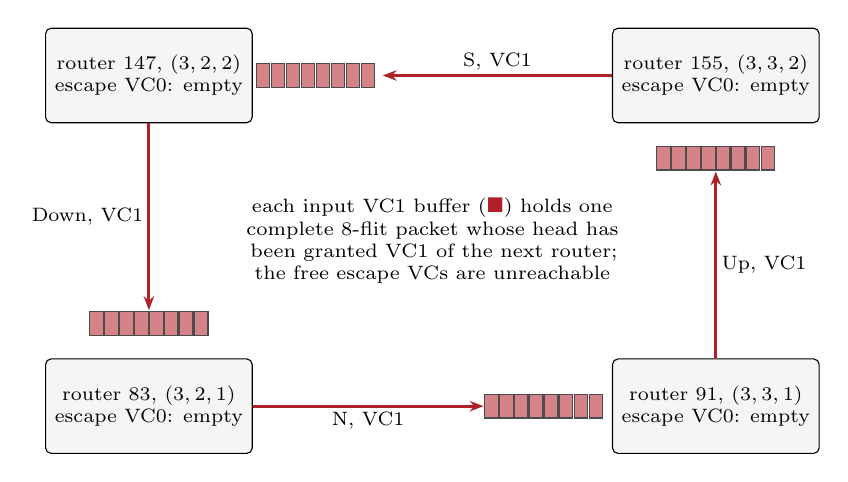
\begin{tikzpicture}[
  rtr/.style={draw=black,fill=black!4,rounded corners=2pt,minimum width=2.6cm,minimum height=1.2cm,align=center,font=\scriptsize},
  slot/.style={draw=black!70,fill=acc!55,minimum width=0.17cm,minimum height=0.3cm,inner sep=0pt},
  com/.style={-{Stealth[length=5pt]},line width=1.1pt,draw=acc},
  lab/.style={font=\scriptsize,inner sep=1.5pt}]
\node[rtr] (A) at (0,0) {router 83, $(3,2,1)$\\ escape VC0: empty};
\node[rtr] (B) at (7.2,0) {router 91, $(3,3,1)$\\ escape VC0: empty};
\node[rtr] (C) at (7.2,4.2) {router 155, $(3,3,2)$\\ escape VC0: empty};
\node[rtr] (D) at (0,4.2) {router 147, $(3,2,2)$\\ escape VC0: empty};
% input VC1 buffers, eight slots each, full
\foreach \i in {0,...,7} \node[slot] at (4.35+\i*0.19,0) {};      % B, from A (north link)
\foreach \i in {0,...,7} \node[slot] at (6.535+\i*0.19,3.15) {};  % C, from B (up link)
\foreach \i in {0,...,7} \node[slot] at (1.45+\i*0.19,4.2) {};    % D, from C (south link)
\foreach \i in {0,...,7} \node[slot] at (-0.665+\i*0.19,1.05) {}; % A, from D (down link)
\draw[com] (A.east) -- node[lab,below]{N, VC1} (4.25,0);
\draw[com] (B.north) -- node[lab,right]{Up, VC1} (7.2,2.98);
\draw[com] (C.west) -- node[lab,above]{S, VC1} (2.97,4.2);
\draw[com] (D.south) -- node[lab,left]{Down, VC1} (0,1.22);
\node[font=\scriptsize,text width=5.4cm,align=center] at (3.6,2.1) {each input VC1 buffer (\textcolor{acc}{$\blacksquare$}) holds one complete 8-flit packet whose head has been granted VC1 of the next router;\\ the free escape VCs are unreachable};
\end{tikzpicture}
\caption{Deadlock witness for minimal adaptive routing with an escape subnetwork under non-atomic VC reallocation (\cls{FA}, $8\times8\times4$ mesh, overload). The cycle lies in the Y--Z plane $x=3$; a second, disjoint cycle was found in the plane $x=0$ of the same run.}
\label{fig:witness}
\end{figure}

\paragraph{BookSim, and why the absence of deadlock there is no guarantee.} BookSim's minimal adaptive routing function has the same routing relation and escape VC as \cls{FA}, and its rule for VC availability under non-atomic reuse (\texttt{wait\_for\_tail\_credit} $=0$) is the same as ours. Yet it completed all \val{na.bs.n} of our batch-mode drain tests (uniform, transpose and bit-reversal traffic on the $4\times4\times4$ mesh, uniform and bit-reversal on $8\times8\times8$; full injection; up to \val{na.bs.maxcycles} cycles) without deadlock, whereas our simulator deadlocked in most comparable runs, including with BookSim's four-cycle hop and with its equal-priority choice among adaptive candidates (\val{na.rsel.8x8x4} runs on $8\times8\times4$, \val{na.rsel.8x8x8} on $8\times8\times8$ with a four-cycle hop). Instrumenting both simulators shows that the hazard is the same and only its frequency differs. Both grant heads adaptive VCs whose downstream buffer is full---the commitment of \cref{prop:nonatomic}---but BookSim does so in \val{na.commit.booksim.888}\% of its VC allocations on the $8\times8\times8$ mesh at full injection (\val{na.commit.booksim.444}\% on $4\times4\times4$), against \val{na.commit.ours.888.h4}\% for our router with the same hop delay (\val{na.commit.ours.444.h4}\% on $4\times4\times4$); since a deadlock requires a closed cycle of such commitments, its probability falls much faster than the commitment rate. We did not isolate the cause of the lower rate. It is not the injection rule: in both simulators a packet may take an adaptive VC at its source router (BookSim's routing function ignores the injection VC), and both rates were measured under this common rule. Plausible causes are BookSim's separate VC- and switch-allocation stages and its allocator, which we did not vary. The frequency is sensitive to incidental details: confining half of the packets to the escape network from their source, a policy that neither simulator uses by default, removed the deadlock from our runs (\val{na.inj1.k} of \val{na.inj1.n} deadlocked, against \val{na.inj0.k} of \val{na.inj0.n} under the default rule). None of this is a guarantee: BookSim reaches the precondition of the deadlock in about one VC allocation in ten, \cref{prop:nonatomic} shows that the commitment cycle is a legal state, and \cref{fig:witness} shows that it is reachable. A design that relies on \cref{thm:duato} must use atomic reallocation, or a scheme such as whole-packet forwarding~\cite{ma2012wpf} that restores its assumption.

% ---------------------------------------------------------------------
\subsection{RQ2: performance and robustness (\D{2}, \D{3}, \D{4}, \D{6}, \D{12})}
\label{sec:rq-perf}

\paragraph{Path diversity (\D{2}).} \Cref{tab:d2} gives the exact path counts. Dimension-order routing admits one path per pair; the fully adaptive relations admit all minimal paths ($\alpha=1$) and more than one for \val{d2.fa.multi}\% of the pairs; negative-first admits on average \val{d2.nf.alpha} of the minimal paths but more than one for \val{d2.nf.multi}\% of pairs; the Hamiltonian relation, which may leave the minimal box, admits \val{d2.ham.median} paths for the median pair. Among VPC classes, elevator-first relations route deterministically once the elevator is chosen, whereas the elevator choice of \cls{AES-G} and \cls{AdEle} creates alternatives for \val{d2.aesg.multi}\% of the pairs. Path diversity is necessary for fault tolerance but, as the next paragraphs show, it is a poor predictor of performance.

\begin{table}[tbp]
\centering
\caption{Path diversity (\D{2}), exact enumeration on the fault-free mesh. $\alpha$: mean fraction of minimal paths admitted (undefined for non-minimal and VPC relations).}
\label{tab:d2}
\small
\begin{tabular}{@{}lrrr@{}}
\toprule
Class & $\alpha$ (minimal paths admitted) & Pairs with $>1$ path & Median paths \\
\midrule
\cls{XYZ} & 0.144 & 0.0\% & 1 \\
\cls{ZXY} & 0.144 & 0.0\% & 1 \\
\cls{NF} & 0.458 & 75.5\% & 5 \\
\cls{DyAD} & 0.458 & 75.5\% & 5 \\
\cls{HAM} & 0.215 & 95.7\% & 3{,}799{,}652 \\
\cls{O1T} & 0.221 & 93.3\% & 2 \\
\cls{ROMM} & 0.480 & 93.3\% & 14 \\
\cls{VAL} & -- & 100.0\% & 250 \\
\cls{FA} & 1.000 & 93.3\% & 30 \\
\cls{RCA} & 1.000 & 93.3\% & 30 \\
\cls{QR} & 1.000 & 93.3\% & 30 \\
\cls{TA} & 1.000 & 93.3\% & 30 \\
\cls{EF} & -- & 0.0\% & 1 \\
\cls{EF-R} & -- & 0.0\% & 1 \\
\cls{AES-G} & -- & 75.3\% & 16 \\
\cls{AdEle} & -- & 75.3\% & 4 \\
\cls{FL} & -- & 45.5\% & 1 \\
\bottomrule
\end{tabular}
\end{table}

\paragraph{Saturation throughput (\D{3}).} \Cref{tab:d3fc,fig:curves} show the classic trade-off with unusual clarity. After the bisection refinement, every saturation throughput is bracketed to within \val{d3.bracket.max}\% (median \val{d3.bracket.median}\%) by the next unstable load; ratios below are point estimates, with the range allowed by the brackets in parentheses. On uniform traffic, \cls{XYZ}, \cls{ZXY}, \cls{FA}, \cls{RCA}, \cls{QR} and \cls{TA} saturate within four percent of each other (\val{d3.sat.ta.random}--\val{d3.sat.xyz.random} flits/node/cycle), because uniform traffic is already balanced by dimension-order routing. On permutations, adaptivity pays: on bit-reversal \cls{FA} saturates at \val{d3.br.fa.over.xyz} times the load of \cls{XYZ} (\val{d3.br.fa.over.xyz.lo}--\val{d3.br.fa.over.xyz.hi}), and on transpose at \val{d3.tr.fa.over.xyz} times (\val{d3.tr.fa.over.xyz.lo}--\val{d3.tr.fa.over.xyz.hi}). The partially adaptive turn-model and Hamiltonian classes do not have this advantage; on uniform traffic they saturate well below \cls{XYZ} (\val{d3.sat.nf.random} and \val{d3.sat.ham.random}), because their asymmetric adaptiveness concentrates traffic. Oblivious routing pays its average distance: \cls{VAL} saturates at \val{d3.sat.val.random}. Vertical-first routing (\cls{ZXY}) multiplies \cls{XYZ}'s bit-reversal saturation throughput by \val{d3.br.zxy.over.xyz} (\val{d3.br.zxy.over.xyz.lo}--\val{d3.br.zxy.over.xyz.hi}) with the same single VC, at a small cost on transpose (\val{d3.sat.zxy.transpose1} against \val{d3.sat.xyz.transpose1}) and at overload (\val{d3.mst.zxy.transpose1} against \val{d3.mst.xyz.transpose1} on transpose). Beyond saturation, adaptive classes lose throughput (overload columns of \cref{tab:d3fc}) whereas dimension-order routing does not: \cls{FA} accepts \val{d3.mst.fa.random} flits/node/cycle at overload against \val{d3.mst.xyz.random} for \cls{XYZ}. The uniform condition of \D{3} requires at least \val{d3.thr.unif} flits/node/cycle; one verdict lies within the residual uncertainty of the brackets, because its bracket overlaps that of the threshold: \cls{O1T} fails at \val{d3.sat.o1t.random}.

\begin{table}[tbp]
\centering
\caption{Performance of 3D-FC classes (\D{3}). Zero-load latency at PIR 0.002; saturation throughput in flits/node/cycle (highest accepted throughput with at most 1\% undelivered and no deadlock, over the coarse sweep and its bisection refinement); overload throughput accepted at an offered load of 0.6 flits/node/cycle.}
\label{tab:d3fc}
\small
\begin{tabular}{@{}lrrrrrrrr@{}}
\toprule
Class & \multicolumn{3}{c}{Zero-load latency (cycles)} & \multicolumn{3}{c}{Saturation throughput} & \multicolumn{2}{c}{Overload throughput} \\
\cmidrule(lr){2-4}\cmidrule(lr){5-7}\cmidrule(lr){8-9}
 & Unif. & Transp. & Bit-rev. & Unif. & Transp. & Bit-rev. & Unif. & Transp. \\
\midrule
\cls{XYZ} & 14.1 & 14.9 & 15.4 & \best{0.328} & 0.147 & 0.056 & 0.330 & 0.209 \\
\cls{ZXY} & 14.1 & 14.9 & 14.2 & 0.318 & 0.142 & 0.146 & 0.323 & 0.197 \\
\cls{NF} & 14.1 & 14.8 & 14.3 & 0.218 & 0.234 & 0.107 & 0.160 & 0.218 \\
\cls{DyAD} & 14.3 & 15.3 & 14.6 & 0.173 & 0.122 & 0.088 & 0.096 & 0.145 \\
\cls{HAM} & 14.1 & 14.8 & 14.2 & 0.252 & 0.166 & 0.179 & 0.131 & 0.107 \\
\cls{O1T} & 14.2 & \second{14.6} & 14.4 & 0.288 & 0.218 & 0.084 & 0.296 & 0.244 \\
\cls{ROMM} & 14.3 & 15.2 & 14.3 & 0.178 & 0.116 & 0.104 & 0.140 & 0.108 \\
\cls{VAL} & 21.8 & 21.9 & 21.8 & 0.126 & 0.125 & 0.124 & 0.129 & 0.077 \\
\cls{FA} & \best{13.8} & \best{14.5} & \second{14.0} & 0.321 & \second{0.263} & 0.261 & 0.265 & 0.223 \\
\cls{RCA} & \best{13.8} & \best{14.5} & \best{13.9} & \second{0.325} & \best{0.270} & \best{0.269} & 0.266 & 0.223 \\
\cls{QR} & \best{13.8} & \best{14.5} & \best{13.9} & 0.319 & 0.262 & \second{0.267} & 0.264 & 0.222 \\
\cls{TA} & \second{14.0} & \second{14.6} & \best{13.9} & 0.316 & 0.251 & 0.262 & 0.264 & 0.222 \\
\bottomrule
\end{tabular}
\end{table}

\begin{figure}[tbp]
\centering
\begin{tikzpicture}
\begin{groupplot}[group style={group size=3 by 1,horizontal sep=1.15cm},
  width=0.355\linewidth,height=5.1cm,xmin=0,ymin=10,ymax=150,
  xlabel={offered load (flits/node/cycle)},
  tick label style={font=\scriptsize},label style={font=\scriptsize},title style={font=\small},
  every axis plot/.append style={line width=0.8pt,mark size=1.4pt}]
\nextgroupplot[title={uniform},ylabel={mean latency (cycles)},xmax=0.36,
  legend to name=curveleg,legend columns=7,legend style={font=\scriptsize,draw=none}]
\curveplot{c6,mark=*}{xyz}{random}\addlegendentry{XYZ}
\curveplot{c2,mark=square*}{zxy}{random}\addlegendentry{ZXY}
\curveplot{c3,mark=triangle*}{nf}{random}\addlegendentry{NF}
\curveplot{c4,mark=diamond*}{ham}{random}\addlegendentry{HAM}
\curveplot{c5,mark=pentagon*}{o1t}{random}\addlegendentry{O1T}
\curveplot{black!50,dashed,mark=o}{val}{random}\addlegendentry{VAL}
\curveplot{c1,mark=*,mark options={fill=white}}{fa}{random}\addlegendentry{FA}
\nextgroupplot[title={transpose},xmax=0.27]
\curveplot{c6,mark=*}{xyz}{transpose1}
\curveplot{c2,mark=square*}{zxy}{transpose1}
\curveplot{c3,mark=triangle*}{nf}{transpose1}
\curveplot{c4,mark=diamond*}{ham}{transpose1}
\curveplot{c5,mark=pentagon*}{o1t}{transpose1}
\curveplot{black!50,dashed,mark=o}{val}{transpose1}
\curveplot{c1,mark=*,mark options={fill=white}}{fa}{transpose1}
\nextgroupplot[title={bit-reversal},xmax=0.29]
\curveplot{c6,mark=*}{xyz}{bitreversal}
\curveplot{c2,mark=square*}{zxy}{bitreversal}
\curveplot{c3,mark=triangle*}{nf}{bitreversal}
\curveplot{c4,mark=diamond*}{ham}{bitreversal}
\curveplot{c5,mark=pentagon*}{o1t}{bitreversal}
\curveplot{black!50,dashed,mark=o}{val}{bitreversal}
\curveplot{c1,mark=*,mark options={fill=white}}{fa}{bitreversal}
\end{groupplot}
\end{tikzpicture}
\pgfplotslegendfromname{curveleg}
\caption{Latency--load curves of eight 3D-FC classes ($8\times8\times4$, coarse sweep, mean of three seeds; points with more than 1\% undelivered packets, with deadlock or with a mean latency above 150 cycles omitted). Adaptivity buys throughput on permutations; on uniform traffic dimension-order routing is as good as any.}
\label{fig:curves}
\end{figure}

Among VPC classes (\cref{tab:d3vpc}), saturation throughput is limited by the elevators: \cls{EF} saturates at \val{d3.sat.ef.random} flits/node/cycle on uniform traffic, less than a quarter of the fully connected mesh, and global-load elevator selection (\cls{AES-G}) raises it to \val{d3.sat.aesg.random}, whereas \cls{AdEle}'s local selection reaches \val{d3.sat.adele.random} and First-Last \val{d3.sat.fl.random}.

With four elevators instead of sixteen (\cref{tab:vpc4}), every VPC class saturates before PIR 0.006 (between \val{vpc4.und.min}\% and \val{vpc4.und.max}\% of the packets undelivered) and the ranking changes. Global elevator selection is still the fastest on uniform traffic, but on transpose First-Last, whose planar sub-routes are adaptive, has the lowest latency at PIR 0.003 (\val{vpc4.fl.transpose1.0.003} cycles against \val{vpc4.ef.transpose1.0.003} for \cls{EF} and \val{vpc4.aesg.transpose1.0.003} for \cls{AES-G}), and \cls{AdEle} saturates first. Global elevator selection pays when there are enough elevators to balance; when every elevator is a bottleneck, planar adaptivity around the elevators matters more.

\begin{table}[tbp]
\centering
\caption{Performance of VPC classes (\D{3}), 16 elevators; definitions as in \cref{tab:d3fc}.}
\label{tab:d3vpc}
\small
\begin{tabular}{@{}lrrrrrrrr@{}}
\toprule
Class & \multicolumn{3}{c}{Zero-load latency (cycles)} & \multicolumn{3}{c}{Saturation throughput} & \multicolumn{2}{c}{Overload throughput} \\
\cmidrule(lr){2-4}\cmidrule(lr){5-7}\cmidrule(lr){8-9}
 & Unif. & Transp. & Bit-rev. & Unif. & Transp. & Bit-rev. & Unif. & Transp. \\
\midrule
\cls{EF} & 15.2 & 17.1 & 15.4 & 0.074 & 0.043 & 0.048 & 0.107 & 0.061 \\
\cls{AES-G} & \best{14.6} & \best{15.7} & \best{14.7} & \best{0.113} & \best{0.068} & \best{0.073} & 0.051 & 0.064 \\
\cls{AdEle} & \second{14.8} & \second{16.3} & \second{15.2} & \second{0.082} & \second{0.060} & \second{0.065} & 0.039 & 0.067 \\
\cls{FL} & 15.4 & 16.9 & 16.1 & 0.080 & 0.058 & 0.051 & 0.015 & 0.058 \\
\bottomrule
\end{tabular}
\end{table}

\begin{table}[tbp]
\centering
\caption{VPC classes with four elevators (stride 4): mean latency (cycles), three seeds. $^\ast$More than 1\% of the packets undelivered (saturated; latency of delivered packets only, not ranked).}
\label{tab:vpc4}
\small
\begin{tabular}{@{}lrrrrrr@{}}
\toprule
Class & \multicolumn{3}{c}{Uniform} & \multicolumn{3}{c}{Transpose} \\
\cmidrule(lr){2-4}\cmidrule(lr){5-7}
PIR & 0.001 & 0.003 & 0.006 & 0.001 & 0.003 & 0.006 \\
\midrule
\cls{EF} & 15.9 & 20.4 & 474.1$^{\ast}$ & 18.2 & \second{69.2} & 668.9$^{\ast}$ \\
\cls{AES-G} & \best{15.2} & \best{18.8} & 557.3$^{\ast}$ & \best{17.6} & 76.6 & 833.6$^{\ast}$ \\
\cls{AdEle} & \second{15.5} & 22.0 & 490.7$^{\ast}$ & \second{18.1} & 329.7$^{\ast}$ & 608.4$^{\ast}$ \\
\cls{FL} & 16.2 & \second{19.7} & 647.2$^{\ast}$ & 18.5 & \best{34.4} & 1246.8$^{\ast}$ \\
\bottomrule
\end{tabular}
\end{table}

\paragraph{Traffic robustness (\D{4}).} Saturation throughput describes one load; \D{4} asks whether a class remains competitive over the whole ERA grid of six patterns and five loads (\cref{tab:d4fc,tab:d4vpc}). Only \cls{ZXY} passes among 3D-FC classes, with a worst ratio of \val{d4.zxy.ratio} to the best class (\val{d4.zxy.worst}). Every adaptive class fails on hotspot traffic: \cls{FA} is \val{d4.hot.fa.over.xyz} times slower than \cls{XYZ} there, and \cls{NF} \val{d4.hot.nf.over.xyz} times. These verdicts rest on a saturated regime. With 20\% of the packets sent to one node, the hot node is oversubscribed from PIR 0.003 on; on average \val{d4.fc.hot.und.0.003}\%, \val{d4.fc.hot.und.0.006}\%, \val{d4.fc.hot.und.0.009}\% and \val{d4.fc.hot.und.0.012}\% of the hotspot packets created in the window are undelivered at PIR 0.003, 0.006, 0.009 and 0.012, and latency covers delivered packets only. The hotspot column therefore compares classes under persistent local overload, not below saturation. Without it, \val{d4.fc.nohot.nflips} 3D-FC classes would pass \D{4} (\val{d4.fc.nohot.flips}; \cls{FA}: \val{d4.fa.ratio.nohot}), whereas \cls{XYZ}, \cls{O1T}, \cls{DyAD} and \cls{VAL} would still fail. A plausible mechanism, which we did not isolate, is tree saturation spread by adaptivity: adaptive packets distribute the congestion around the hot node over all minimal paths towards it, so that background traffic crossing that region is blocked in every dimension instead of one. \cls{XYZ} fails on bit-reversal, where it is \val{d4.br.xyz.over.zxy} times slower than \cls{ZXY}, and \cls{O1T} also fails there (\val{d4.o1t.ratio}$\times$). Among VPC classes only \cls{AES-G} passes (\val{d4.aesg.ratio}$\times$, worst on transpose); \cls{EF}, \cls{AdEle} and \cls{FL} exceed the best class by factors of \val{d4.ef.ratio}, \val{d4.adele.ratio} and \val{d4.fl.ratio}.

\begin{table}[tbp]
\centering
\caption{Traffic robustness of 3D-FC classes (\D{4}). Mean latency (cycles) of delivered packets over five loads and five seeds; worst ratio to the best class of the family. Hotspot runs are saturated at PIR $\ge0.003$.}
\label{tab:d4fc}
\small
\setlength{\tabcolsep}{4pt}
\begin{tabular}{@{}lrrrrrrrc@{}}
\toprule
Class & Uniform & Transpose & Shuffle & Bit-rev. & Butterfly & Hotspot & Worst ratio & D4 \\
\midrule
\cls{XYZ} & 15.6 & 16.9 & 13.9 & 176.9 & 10.6 & \best{531.0} & 12.17 (Bit-rev.) & \xmark \\
\cls{ZXY} & 15.6 & 16.9 & 14.4 & 16.3 & 10.6 & \second{561.8} & 1.14 (Shuffle) & \cmark \\
\cls{NF} & 15.6 & 16.6 & 13.6 & 17.4 & 10.6 & 3492.6 & 6.58 (Hotspot) & \xmark \\
\cls{DyAD} & 16.5 & 22.4 & 14.1 & 29.9 & 10.6 & 3373.1 & 6.35 (Hotspot) & \xmark \\
\cls{HAM} & 15.5 & 16.6 & 13.6 & 15.6 & \best{10.3} & 2382.1 & 4.49 (Hotspot) & \xmark \\
\cls{O1T} & 15.8 & 15.8 & 14.0 & 77.7 & \second{10.4} & 1129.8 & 5.35 (Bit-rev.) & \xmark \\
\cls{ROMM} & 16.5 & 19.3 & 13.9 & 18.3 & 10.5 & 3284.0 & 6.18 (Hotspot) & \xmark \\
\cls{VAL} & 29.1 & 29.4 & 28.6 & 28.3 & 23.8 & 3585.8 & 6.75 (Hotspot) & \xmark \\
\cls{FA} & \best{14.6} & \best{15.2} & 12.9 & 15.1 & 10.6 & 2257.0 & 4.25 (Hotspot) & \xmark \\
\cls{RCA} & \second{14.7} & \second{15.4} & \second{12.8} & \second{14.7} & 10.5 & 2261.5 & 4.26 (Hotspot) & \xmark \\
\cls{QR} & \second{14.7} & 15.5 & \best{12.7} & \best{14.5} & \second{10.4} & 2251.8 & 4.24 (Hotspot) & \xmark \\
\cls{TA} & 15.1 & 15.9 & 13.2 & 15.0 & \second{10.4} & 2220.6 & 4.18 (Hotspot) & \xmark \\
\bottomrule
\end{tabular}
\end{table}

\begin{table}[tbp]
\centering
\caption{Traffic robustness of VPC classes (\D{4}); definitions as in \cref{tab:d4fc}.}
\label{tab:d4vpc}
\small
\setlength{\tabcolsep}{4pt}
\begin{tabular}{@{}lrrrrrrrc@{}}
\toprule
Class & Uniform & Transpose & Shuffle & Bit-rev. & Butterfly & Hotspot & Worst ratio & D4 \\
\midrule
\cls{EF} & 96.4 & 273.3 & 80.4 & 114.7 & 21.5 & \best{978.8} & 5.42 (Shuffle) & \xmark \\
\cls{AES-G} & \best{18.1} & 282.9 & \best{14.9} & \best{103.4} & \best{12.3} & 1193.1 & 1.26 (Transpose) & \cmark \\
\cls{AdEle} & \second{88.8} & \second{236.1} & \second{37.2} & \second{105.1} & \second{12.9} & 1440.5 & 4.91 (Uniform) & \xmark \\
\cls{FL} & 233.1 & \best{223.7} & 145.0 & 261.9 & 27.8 & \second{1170.1} & 12.89 (Uniform) & \xmark \\
\bottomrule
\end{tabular}
\end{table}

Self-similar traffic (\cref{tab:burst}) sharpens the picture at the tail. At PIR 0.012 the minimal adaptive classes have the lowest 99th-percentile latency (\cls{FA}: \val{d4.burst.fa.p99} cycles against \val{d4.burst.xyz.p99} for \cls{XYZ}), Valiant's tail explodes (\val{d4.burst.val.p99}). In VPC stacks bursty traffic saturates the elevators: at PIR 0.009 only global elevator selection remains stable (\val{d4.burst.aesg.lat9} cycles, against \val{d4.burst.ef.und9}\% of the packets undelivered for \cls{EF} and \val{d4.burst.adele.und9}\% for \cls{AdEle}), and at PIR 0.012 every VPC class is saturated.

\begin{table}[tbp]
\centering
\caption{Self-similar (ON/OFF Pareto) traffic: mean and 99th-percentile latency (cycles), five seeds. $^\ast$More than 1\% of the packets undelivered (saturated; delivered packets only, not ranked).}
\label{tab:burst}
\small
\begin{tabular}{@{}lrrrr@{}}
\toprule
Class & \multicolumn{2}{c}{Mean latency} & \multicolumn{2}{c}{99th-percentile latency} \\
\cmidrule(lr){2-3}\cmidrule(lr){4-5}
 & PIR 0.009 & PIR 0.012 & PIR 0.009 & PIR 0.012 \\
\midrule
\cls{XYZ} & 21.4 & 29.6 & 57.0 & 129.4 \\
\cls{ZXY} & 20.5 & 25.6 & 47.4 & 72.6 \\
\cls{NF} & 20.8 & 26.5 & 48.8 & 80.2 \\
\cls{DyAD} & 23.1 & 32.4 & 65.2 & 133.5 \\
\cls{HAM} & 20.5 & 25.5 & 46.2 & 69.8 \\
\cls{O1T} & 21.9 & 29.9 & 56.4 & 104.2 \\
\cls{ROMM} & 23.9 & 40.8 & 70.4 & 264.2 \\
\cls{VAL} & 56.5 & 213.1 & 397.0 & 2908.5 \\
\cls{FA} & \best{18.6} & \best{22.8} & \best{41.6} & \best{62.8} \\
\cls{RCA} & 18.8 & \second{23.0} & \best{41.6} & 63.2 \\
\cls{QR} & \second{18.7} & \second{23.0} & \second{41.8} & \second{63.0} \\
\cls{TA} & 19.6 & 24.1 & 44.0 & 64.7 \\
\midrule
\cls{EF} & 296.8$^{\ast}$ & 883.7$^{\ast}$ & 5297.3$^{\ast}$ & 9600.6$^{\ast}$ \\
\cls{AES-G} & 27.4 & 298.8$^{\ast}$ & 85.8 & 4272.2$^{\ast}$ \\
\cls{AdEle} & 245.2$^{\ast}$ & 920.0$^{\ast}$ & 4775.3$^{\ast}$ & 10468.5$^{\ast}$ \\
\cls{FL} & 878.6$^{\ast}$ & 1588.1$^{\ast}$ & 9437.9$^{\ast}$ & 12867.6$^{\ast}$ \\
\bottomrule
\end{tabular}
\end{table}

\paragraph{Load balance and fairness (\D{6}).} No class passes \D{6} (\cref{tab:d6}). On router load, dimension-order routing balances uniform traffic best (Jain index \val{d6.xyz.jain} for \cls{XYZ}, \val{d6.zxy.jain} for \cls{ZXY} and \cls{O1T}); the partially adaptive and oblivious classes are lower (\val{d6.nf.jain} for \cls{NF}, \val{d6.romm.jain} for \cls{ROMM}), and the VPC classes, whose elevators concentrate load by construction, lower still (\val{d6.ef.jain} for \cls{EF}). The fairness condition fails for every class: the minimum over stress runs of the per-source accepted-throughput Jain index is at most \val{d6.best.src.v} (\cls{\val{d6.best.src}}) among classes that do not deadlock---individual runs at the lowest stress load reach \val{d6.srcjain.maxrun}---and the longest wait for VC allocation exceeds 10,000 cycles, two thirds of the run, in \val{d6.va.over10k} classes. The routing class matters: the minimum ranges from \val{d6.srcjain.min.lo} (\cls{\val{d6.srcjain.min.lo.class}}) to \val{d6.best.src.v}, with \cls{XYZ} at \val{d6.xyz.srcjain} and \cls{FA} at \val{d6.fa.srcjain}. That no class reaches 0.95 is consistent with the parking-lot effect of the locally fair round-robin arbitration that all classes share (\cref{sec:bg-router}); whether age-based or frame-based arbitration would let some class pass is untested here.

\begin{table}[tbp]
\centering
\caption{Load balance and fairness (\D{6}). Router-load Jain index on uniform traffic (ERA grid); per-source accepted-throughput Jain index (minimum) and max/mean source latency (mean) over stress runs on uniform traffic; longest VC-allocation wait.}
\label{tab:d6}
\small
\begin{tabular}{@{}lrrrrc@{}}
\toprule
Class & Router-load Jain & Source-throughput Jain & Max/mean source latency & Max VA wait & D6 \\
 & (uniform, grid) & (stress, min.) & (stress, mean) & (cycles) & \\
\midrule
\cls{XYZ} & 0.959 & 0.528 & 2.35 & 14{,}831 & \xmark \\
\cls{ZXY} & 0.958 & 0.537 & 2.16 & 7{,}139 & \xmark \\
\cls{NF} & 0.886 & 0.235 & 9.70 & 14{,}782 & \xmark \\
\cls{DyAD} & 0.893 & 0.116 & 2.32 & 14{,}922 & \xmark \\
\cls{HAM} & 0.910 & 0.184 & 1.93 & 14{,}794 & \xmark \\
\cls{O1T} & 0.958 & 0.862 & 1.81 & 3{,}738 & \xmark \\
\cls{ROMM} & 0.906 & 0.229 & 3.03 & 14{,}935 & \xmark \\
\cls{VAL} & 0.951 & 0.258 & 2.29 & 14{,}916 & \xmark \\
\cls{FA} & 0.949 & 0.413 & 2.12 & 14{,}856 & \xmark \\
\cls{RCA} & 0.951 & 0.411 & 2.14 & 14{,}791 & \xmark \\
\cls{QR} & 0.945 & 0.413 & 2.14 & 14{,}557 & \xmark \\
\cls{TA} & 0.870 & 0.412 & 2.13 & 14{,}855 & \xmark \\
\midrule
\cls{EF} & 0.750 & 0.159 & 2.75 & 14{,}979 & \xmark \\
\cls{AES-G} & 0.774 & 0.093 & 2.64 & 14{,}722 & \xmark \\
\cls{AdEle} & 0.773 & 0.037 & 2.10 & 14{,}932 & \xmark \\
\cls{FL} & 0.677 & 0.023 & 1.99 & 14{,}832 & \xmark \\
\bottomrule
\end{tabular}
\end{table}

\paragraph{Robustness of conclusions (\D{12}).} \Cref{tab:d12} re-runs every class under eight router variants. Conclusions about uniform traffic are robust: every class keeps the sign of its difference with the reference in all variants. Conclusions about transpose are not: \val{d12.nflips} classes change sign in at least one variant (\val{d12.flips}). Under the deadlock rule, the escape-based classes, which deadlocked under non-atomic reallocation, fail \D{12} as well. Two limits apply. The depth-16 variant is degenerate: with atomic reallocation and eight-flit packets a VC buffer never holds more than one packet, so slots beyond the eighth are never used, and its results equal the baseline's in \val{d12.d16.same} of \val{d12.d16.n} runs (all except overload runs of \cls{\val{d12.d16.diff.classes}}); \D{12} therefore rests on seven effective variants. And the sign test uses two seeds without a noise tolerance; the median seed-to-seed standard deviation of overload throughput is \val{d12.seed.sd.median} flits/node/cycle, and treating differences below 0.01 as ties would let four more classes pass (\cref{tab:thresh}). Doubling the VCs, for instance, raises the overload throughput of \cls{XYZ} from \val{d12.xyz.base} to \val{d12.xyz.v4} flits/node/cycle but lowers that of \cls{FA} from \val{d12.fa.base} to \val{d12.fa.v4}; non-atomic reallocation raises it for almost every class (\cls{FA}: \val{d12.fa.na}) while making the escape-based ones deadlock. Claims that an adaptive selection beats a deterministic one on a permutation are, in other words, conditional on the router; papers should report them with the router parameters that produced them.

\begin{table}[tbp]
\centering
\caption{Robustness of conclusions (\D{12}). Accepted throughput at overload (uniform, offered 0.6 flits/node/cycle, two seeds) under eight router variants, and number of variants in which the class is above/below the reference on uniform and transpose traffic (exact ties counted in neither column). $^\ddagger$At least one deadlocked run.}
\label{tab:d12}
\scriptsize
\setlength{\tabcolsep}{3pt}
\begin{tabular}{@{}lrrrrrrrrccc@{}}
\toprule
Class & \multicolumn{8}{c}{Accepted throughput at overload, uniform (flits/node/cycle)} & \multicolumn{2}{c}{Sign vs.\ ref.\ ($+/-$)} & D12 \\
\cmidrule(lr){2-9}\cmidrule(lr){10-11}
 & baseline & 4 VCs & non-atomic & depth 4 & depth 16 & 4-flit pkts & 16-flit pkts & 3-cycle hop & Unif. & Transp. & \\
\midrule
\cls{XYZ} & 0.330 & 0.368 & 0.371 & 0.319 & 0.330 & 0.321 & 0.326 & 0.286 & -- & -- & ref \\
\cls{ZXY} & 0.323 & 0.360 & 0.359 & 0.305 & 0.323 & 0.313 & 0.311 & 0.282 & 0/8 & 0/8 & \cmark \\
\cls{NF} & 0.160 & 0.160 & 0.181 & 0.175 & 0.160 & 0.142 & 0.179 & 0.132 & 0/8 & 5/3 & \xmark \\
\cls{DyAD} & 0.096 & 0.088 & 0.150 & 0.127 & 0.034 & 0.018 & 0.129 & 0.082 & 0/8 & 1/7 & \xmark \\
\cls{HAM} & 0.131 & 0.134 & 0.156 & 0.140 & 0.131 & 0.118 & 0.143 & 0.106 & 0/8 & 0/8 & \cmark \\
\cls{O1T} & 0.296 & 0.363 & 0.345 & 0.273 & 0.296 & 0.283 & 0.280 & 0.255 & 0/8 & 7/1 & \xmark \\
\cls{ROMM} & 0.140 & 0.153 & 0.172 & 0.143 & 0.140 & 0.129 & 0.141 & 0.121 & 0/8 & 0/8 & \cmark \\
\cls{VAL} & 0.129 & 0.169 & 0.155 & 0.114 & 0.129 & 0.123 & 0.118 & 0.109 & 0/8 & 0/8 & \cmark \\
\cls{FA} & 0.265 & 0.230 & 0.318$^{\ddagger}$ & 0.259 & 0.265 & 0.258 & 0.271 & 0.220 & 0/8 & 4/3 & \xmark$^{\ddagger}$ \\
\cls{RCA} & 0.266 & 0.230 & 0.317$^{\ddagger}$ & 0.260 & 0.266 & 0.258 & 0.271 & 0.220 & 0/8 & 4/4 & \xmark$^{\ddagger}$ \\
\cls{QR} & 0.264 & 0.227 & 0.314$^{\ddagger}$ & 0.259 & 0.264 & 0.258 & 0.271 & 0.219 & 0/8 & 4/4 & \xmark$^{\ddagger}$ \\
\cls{TA} & 0.264 & 0.230 & 0.317$^{\ddagger}$ & 0.259 & 0.264 & 0.257 & 0.270 & 0.220 & 0/8 & 4/4 & \xmark$^{\ddagger}$ \\
\midrule
\cls{EF} & 0.107 & 0.136 & 0.127 & 0.101 & 0.107 & 0.093 & 0.106 & 0.083 & -- & -- & ref \\
\cls{AES-G} & 0.051 & 0.060 & 0.074 & 0.063 & 0.051 & 0.037 & 0.068 & 0.049 & 0/8 & 6/2 & \xmark \\
\cls{AdEle} & 0.039 & 0.041 & 0.051 & 0.047 & 0.039 & 0.036 & 0.049 & 0.027 & 0/8 & 4/4 & \xmark \\
\cls{FL} & 0.015 & 0.014 & 0.016 & 0.018 & 0.015 & 0.014 & 0.016 & 0.013 & 0/8 & 2/6 & \xmark \\
\bottomrule
\end{tabular}
\end{table}

\paragraph{Scalability.} \Cref{tab:scal} varies the mesh from 64 to 1,024 routers. Size changes the ranking at overload. On uniform traffic the minimal adaptive classes accept the most traffic only on the smallest mesh; from $8\times8\times4$ upwards dimension-order routing accepts more (\cls{XYZ}: \val{d12.scal.xyz.random.16164}, \cls{ZXY}: \val{d12.scal.zxy.random.16164}, \cls{FA}: \val{d12.scal.fa.random.16164} flits/node/cycle on $16\times16\times4$). On bit-reversal the minimal adaptive classes with escape (\cls{FA}, \cls{RCA}, \cls{QR}, \cls{TA}) lead on three of the four meshes, within one percent of each other, but on $8\times8\times8$ \cls{ZXY} accepts as much (\cls{ZXY}: \val{d12.scal.zxy.bitreversal.888}, \cls{FA}: \val{d12.scal.fa.bitreversal.888}). On transpose \cls{O1T} leads on every mesh except the smallest (\val{d12.scal.o1t.transpose1.16164} against \val{d12.scal.fa.transpose1.16164} for \cls{FA} on $16\times16\times4$).

\begin{table}[tbp]
\centering
\caption{Scalability: accepted throughput at overload (offered 0.6 flits/node/cycle; flits/node/cycle) for four mesh sizes, two seeds.}
\label{tab:scal}
\scriptsize
\setlength{\tabcolsep}{3.5pt}
\begin{tabular}{@{}lrrrrrrrrrrrr@{}}
\toprule
Class & \multicolumn{4}{c}{Uniform} & \multicolumn{4}{c}{Transpose} & \multicolumn{4}{c}{Bit-reversal} \\
\cmidrule(lr){2-5}\cmidrule(lr){6-9}\cmidrule(lr){10-13}
 & $4^3$ & $8^2{\times}4$ & $8^3$ & $16^2{\times}4$ & $4^3$ & $8^2{\times}4$ & $8^3$ & $16^2{\times}4$ & $4^3$ & $8^2{\times}4$ & $8^3$ & $16^2{\times}4$ \\
\midrule
\cls{XYZ} & 0.579 & \best{0.330} & \second{0.307} & \second{0.154} & 0.366 & 0.209 & 0.103 & 0.112 & 0.265 & 0.136 & 0.103 & 0.069 \\
\cls{ZXY} & 0.581 & \second{0.323} & \best{0.315} & \best{0.159} & 0.341 & 0.197 & \second{0.130} & 0.104 & 0.388 & 0.180 & \best{0.184} & 0.081 \\
\cls{NF} & 0.444 & 0.160 & 0.119 & 0.045 & 0.361 & 0.218 & 0.108 & 0.103 & 0.350 & 0.185 & 0.173 & 0.101 \\
\cls{DyAD} & 0.292 & 0.096 & 0.075 & 0.028 & 0.319 & 0.145 & 0.099 & 0.079 & 0.327 & 0.175 & 0.142 & 0.092 \\
\cls{HAM} & 0.350 & 0.131 & 0.133 & 0.049 & 0.268 & 0.107 & 0.105 & 0.051 & 0.403 & 0.164 & 0.129 & 0.058 \\
\cls{O1T} & 0.501 & 0.296 & 0.269 & \second{0.154} & \best{0.375} & \best{0.244} & \best{0.150} & \best{0.142} & 0.315 & 0.166 & 0.141 & 0.083 \\
\cls{ROMM} & 0.325 & 0.140 & 0.103 & 0.059 & 0.200 & 0.108 & 0.056 & 0.055 & 0.319 & 0.173 & 0.111 & 0.089 \\
\cls{VAL} & 0.234 & 0.129 & 0.113 & 0.067 & 0.167 & 0.077 & 0.048 & 0.053 & 0.219 & 0.104 & 0.100 & 0.057 \\
\cls{FA} & \second{0.598} & 0.265 & 0.234 & 0.120 & \second{0.374} & \second{0.223} & 0.117 & \second{0.120} & \second{0.516} & \second{0.306} & \best{0.184} & \second{0.148} \\
\cls{RCA} & \best{0.599} & 0.266 & 0.234 & 0.119 & \second{0.374} & \second{0.223} & 0.117 & \second{0.120} & \best{0.517} & \best{0.307} & 0.182 & \second{0.148} \\
\cls{QR} & 0.596 & 0.264 & 0.234 & 0.119 & \second{0.374} & 0.222 & 0.117 & \second{0.120} & \second{0.516} & \second{0.306} & \best{0.184} & \best{0.149} \\
\cls{TA} & 0.596 & 0.264 & 0.234 & 0.119 & \second{0.374} & 0.222 & 0.117 & \second{0.120} & 0.514 & 0.304 & \second{0.183} & \second{0.148} \\
\bottomrule
\end{tabular}
\end{table}

% ---------------------------------------------------------------------
\subsection{RQ3: fault tolerance (\D{5})}
\label{sec:rq-fault}

\Cref{tab:d5fc} gives the exact reachability of every 3D-FC policy, averaged over 2,000 fault maps per configuration. Four results stand out.

\emph{Under planar faults a single path is fragile and a long one more so; adaptivity recovers much of the loss, and locality limits the recovery.} At $p_h=0.1$, \cls{XYZ} delivers \val{d5.xyz.0.1.0.0} of the pairs and \cls{VAL} only \val{d5.val.0.1.0.0}; local minimal adaptive routing \val{d5.min_greedy.0.1.0.0}; the oracle version of the same relation \val{d5.min_oracle.0.1.0.0}; and the connectivity bound is \val{d5.connected.0.1.0.0}. The gap between local and oracle variants---\val{d5.min_greedy.0.1.0.0} versus \val{d5.min_oracle.0.1.0.0}---is the price of making decisions without knowing the faults ahead; closing it requires fault information beyond the neighbourhood or the ability to backtrack.

\emph{Vertical faults favour different policies than planar faults.} Ordering the minimal ports as X, Y, Z is the best local policy under planar faults (\val{d5.min_order.0.1.0.0} at $p_h=0.1$) and no better than \cls{XYZ} under vertical faults (\val{d5.min_order.0.0.2.0} at $p_v=0.2$): taking the vertical hop last leaves no alternative when it fails. The Hamiltonian policy, which may leave the minimal box, is the most robust local policy under vertical faults (\val{d5.ham_greedy.0.0.2.0}).

\emph{Correlation hurts the policies that adapt.} As \cref{thm:corr} predicts, the reachability of the policies it covers is unchanged by correlation (\cls{XYZ}: \val{d5.corr.xyz.0.2} at $p_v=0.2$, within Monte Carlo error); \cls{VAL}, whose two-phase paths may cross a boundary twice and which the theorem does not cover, gains slightly (\val{d5.val.0.0.2.0} to \val{d5.val.0.0.2.4}). Local adaptive policies lose: \val{d5.corr.min_greedy.0.2} for minimal adaptive routing and \val{d5.corr.ham_greedy.0.2} for the Hamiltonian policy at $p_v=0.2$, and up to \val{d5.corr.min_greedy.0.3} at $p_v=0.3$. Clustered faults remove the alternatives that adaptive routing counts on: the healthy columns next to a failed one are likely to have failed too. A fault-tolerance claim established under independent faults overstates the benefit of adaptivity, although in our configurations the overstatement does not change any \D{5} verdict or the ranking of the policies.

\emph{Under moderate faults the losses are the routing's, not the topology's---until the stack partitions.} The connectivity bound is at least \val{d5.conn.min} in every configuration of \cref{tab:d5fc}, so the losses of all policies are self-inflicted. But the bound hides the partition risk quantified in \cref{tab:partition}, which is negligible for independent faults and not for correlated ones.

\begin{table}[tbp]
\centering
\caption{Fault tolerance of 3D-FC policies (\D{5}): exact mean pair reachability over 2,000 fault maps per configuration ($8\times8\times4$). Planar faults with probability $p_h$; vertical faults with marginal $p_v$ and correlation length $\xi$. Local: uniform choice among healthy admissible ports, no backtracking; oracle: some admissible healthy path exists.}
\label{tab:d5fc}
\scriptsize
\setlength{\tabcolsep}{3pt}
\begin{tabular}{@{}lrrrrrrrrr@{}}
\toprule
Policy & \multicolumn{3}{c}{Planar faults, $p_h$} & \multicolumn{6}{c}{Vertical faults, $p_v$ ($\xi$)} \\
\cmidrule(lr){2-4}\cmidrule(lr){5-10}
 & 0.02 & 0.05 & 0.1 & 0.1 (0) & 0.1 (4) & 0.2 (0) & 0.2 (4) & 0.3 (0) & 0.3 (4) \\
\midrule
\cls{XYZ} & 0.900 & 0.771 & 0.596 & 0.881 & 0.879 & 0.774 & 0.772 & 0.677 & 0.670 \\
\cls{ZXY} & 0.900 & 0.771 & 0.596 & 0.881 & 0.879 & 0.774 & 0.772 & 0.677 & 0.670 \\
\cls{O1T} & 0.900 & 0.771 & 0.596 & 0.881 & 0.879 & 0.774 & 0.772 & 0.677 & 0.670 \\
\cls{ROMM} & 0.900 & 0.771 & 0.595 & 0.881 & 0.879 & 0.774 & 0.772 & 0.676 & 0.670 \\
\cls{VAL} & 0.813 & 0.599 & 0.362 & 0.778 & 0.784 & 0.603 & 0.615 & 0.462 & 0.472 \\
\cls{NF}, \cls{DyAD} (local) & 0.933 & 0.840 & 0.702 & 0.938 & 0.922 & 0.873 & 0.839 & 0.805 & 0.751 \\
NF (oracle) & 0.963 & 0.909 & 0.822 & 0.960 & 0.943 & 0.918 & 0.878 & 0.873 & 0.805 \\
\cls{HAM} (local) & 0.964 & 0.907 & 0.801 & 0.997 & 0.987 & 0.992 & 0.962 & 0.984 & 0.921 \\
HAM (oracle) & 0.991 & 0.976 & 0.942 & 0.998 & 0.994 & 0.994 & 0.985 & 0.990 & 0.967 \\
min.\ adaptive, X--Y--Z port order (local) & 0.985 & 0.958 & 0.907 & 0.881 & 0.879 & 0.774 & 0.772 & 0.677 & 0.670 \\
min.\ adaptive, local (\cls{FA}, \cls{RCA}, \cls{QR}, \cls{TA}) & 0.956 & 0.892 & 0.786 & 0.972 & 0.951 & 0.936 & 0.887 & 0.889 & 0.810 \\
min.\ adaptive (oracle) & 0.996 & 0.988 & 0.968 & 0.997 & 0.984 & 0.992 & 0.955 & 0.983 & 0.913 \\
\midrule
connectivity bound (any routing) & 1.000 & 1.000 & 1.000 & 1.000 & 1.000 & 1.000 & 1.000 & 1.000 & 0.999 \\
\bottomrule
\end{tabular}
\end{table}

\paragraph{VPC stacks.} In simulation (\cref{tab:d5vpc}), static elevator assignment loses every packet whose elevator column is broken: \cls{EF} and \cls{FL} drop \val{d5.vpc.ef.0.2.0.drop} of all packets at $p_v=0.2$, and \cls{AdEle}, whose offline subsets do not know the faults, \val{d5.vpc.adele.0.2.0.drop}. Only fault-aware selection is lossless: \cls{EF-R} redirects packets to the nearest healthy elevator at a high latency cost (\val{d5.vpc.efr.0.2.0.lat} cycles against \val{d5.vpc.aesg.0.2.0.lat} for \cls{AES-G}), and \cls{AES-G}, whose global view includes the fault map, is both lossless and fast. Five fault maps per configuration are a small sample, so we computed the exact expected loss of \cls{EF} under uniform traffic for each map, by replaying the simulator's fault sampler: each of the 20 simulated \cls{EF} runs under uniform traffic lies within \val{fcheck.run.max} of the exact value for its map, which validates the fault path of the simulator (\cref{tab:d5vpc} also pools transpose runs, which this check does not cover). Over \val{fcheck.maps} maps, the expected loss is \val{fcheck.0.1.0.mean} for $\xi=0$ and \val{fcheck.0.1.4.mean} for $\xi=4$ at $p_v=0.1$, and \val{fcheck.0.2.0.mean} and \val{fcheck.0.2.4.mean} at $p_v=0.2$---the invariance of \cref{thm:corr}---while its standard deviation across maps rises from \val{fcheck.0.1.0.sd} to \val{fcheck.0.1.4.sd} and from \val{fcheck.0.2.0.sd} to \val{fcheck.0.2.4.sd}. Correlation does not make static assignment worse on average; it makes the loss of an individual chip far less predictable. The differences between the simulated means of \cref{tab:d5vpc} for $\xi=0$ and $\xi=4$ are therefore sampling effects of the five maps. The latencies of lossy classes are those of delivered packets only and are therefore biased downwards; they must not be compared with those of lossless classes.

\begin{table}[tbp]
\centering
\caption{VPC classes under correlated TSV faults (\D{5}), 16 elevators, PIR 0.006, uniform and transpose traffic, five seeds. Loss: fraction of injected packets dropped because the assigned elevator column is broken. $S_{\mathrm{eff}}^{\mathrm{TSV}}$: effective number of TSV columns used (ERA).}
\label{tab:d5vpc}
\small
\begin{tabular}{@{}lrrrrrrc@{}}
\toprule
Class & \multicolumn{3}{c}{$p_v=0.2$, $\xi=0$} & \multicolumn{3}{c}{$p_v=0.2$, $\xi=4$} & D5 \\
\cmidrule(lr){2-4}\cmidrule(lr){5-7}
 & loss & latency & $S_{\mathrm{eff}}^{\mathrm{TSV}}$ & loss & latency & $S_{\mathrm{eff}}^{\mathrm{TSV}}$ & \\
\midrule
\cls{EF} & 0.259 & 63.8 & 10.7 & 0.205 & 78.8 & 11.3 & \xmark \\
\cls{EF-R} & 0.000 & 127.9 & 10.6 & 0.000 & 123.0 & 11.2 & \cmark \\
\cls{AES-G} & 0.000 & 33.9 & 11.9 & 0.000 & 24.6 & 12.3 & \cmark \\
\cls{AdEle} & 0.293 & 19.7 & 11.4 & 0.237 & 20.6 & 11.9 & \xmark \\
\cls{FL} & 0.259 & 21.9 & 10.5 & 0.205 & 22.2 & 11.1 & \xmark \\
\bottomrule
\end{tabular}
\end{table}

% ---------------------------------------------------------------------
\subsection{RQ4: what structural analysis reveals (\D{7})}
\label{sec:rq-structure}

ERA analyses the \val{n.traced} traced runs at the level of resources and time windows. Three of its observations change the interpretation of scalar results.

\emph{Hotspot signatures.} Under hotspot traffic all classes have similar average buffer-pressure entropy, but they differ in how congestion moves (\cref{tab:era}). Relative to \cls{XYZ}, the classes that choose among many paths inside the minimal box---adaptively or, like \cls{ROMM}, obliviously---raise the space--time mutual information by a factor of \val{d7.mi.adapt.min} (\cls{\val{d7.mi.adapt.min.class}}) to \val{d7.mi.adapt.max} (\cls{\val{d7.mi.adapt.max.class}}; \cls{FA}: \val{d7.hot.fa.mi.ratio}) and the window-to-window drift of the activity map (\cls{DyAD}: \val{d7.hot.dyad.jsd.ratio}$\times$): congestion around the hot node migrates over time instead of staying on fixed paths. Classes with few fixed paths (\cls{ZXY}, \cls{O1T}) or with network-wide randomisation (\cls{VAL}) stay close to \cls{XYZ}. This migration co-occurs with the latency penalty of adaptive routing under hotspot traffic (\D{4}) and with its amplification of flooding attacks (\D{11}); our data establish the association, not a causal link, and all these runs are saturated at the hot node.

\emph{Elevator usage.} In VPC stacks, ERA's effective number of TSV columns used shows how evenly the elevators are exploited. On uniform traffic all elevator classes use between \val{d7.vpc.fl.cols} and \val{d7.vpc.adele.cols} of the 16 columns effectively; under hotspot traffic First-Last collapses to \val{d7.vpchot.fl.cols} effective columns and \cls{EF} to \val{d7.vpchot.ef.cols}, whereas \cls{AES-G} keeps \val{d7.vpchot.aesg.cols}, which is consistent with the robustness of global elevator selection.

\emph{Limits of the structural metrics.} Two properties of ERA deserve caution in any evaluation that uses it, ours included. First, temporal metrics depend on the window length: re-running the same configurations and seeds with windows of 250 to 2,000 cycles changes the mutual information by a factor of up to \val{d7.win.mi.ratio} and the Jensen--Shannon drift by up to \val{d7.win.jsd.ratio}, while spatial entropies are unaffected. Temporal ERA metrics are comparable only at equal window length, which must be reported. Second, with traces of this length the permutation test of space--time independence rejects in \val{d7.perm.bh.pct}\% of the \val{d7.perm.n} traced runs after Benjamini--Hochberg correction (smallest attainable $p$ = \val{d7.perm.min.p} with 200 permutations): significance is guaranteed and uninformative, and effect sizes ($\kappa_{ST}$, mutual information) are what discriminate classes.

\begin{table}[tbp]
\centering
\caption{Structural signatures (ERA). Left: hotspot traffic, ratios to \cls{XYZ} of the space--time mutual information and of the mean Jensen--Shannon drift between windows, and normalised buffer-pressure entropy $\hfull{C}$. Right: effective number of TSV columns used by VPC classes (of 16).}
\label{tab:era}
\small
\begin{tabular}{@{}lrrr@{\hspace{1.4em}}lrr@{}}
\toprule
\multicolumn{4}{c}{3D-FC, hotspot traffic} & \multicolumn{3}{c}{VPC, $S_{\mathrm{eff}}^{\mathrm{TSV}}$} \\
\cmidrule(r){1-4}\cmidrule(l){5-7}
Class & MI ratio & JSD ratio & $\hfull{C}$ & Class & uniform & hotspot \\
\midrule
\cls{XYZ} & \val{d7.hot.xyz.mi.ratio} & \val{d7.hot.xyz.jsd.ratio} & \val{d7.hot.xyz.hc} & \cls{EF} & \val{d7.vpc.ef.cols} & \val{d7.vpchot.ef.cols} \\
\cls{ZXY} & \val{d7.hot.zxy.mi.ratio} & \val{d7.hot.zxy.jsd.ratio} & \val{d7.hot.zxy.hc} & \cls{AES-G} & \val{d7.vpc.aesg.cols} & \val{d7.vpchot.aesg.cols} \\
\cls{O1T} & \val{d7.hot.o1t.mi.ratio} & \val{d7.hot.o1t.jsd.ratio} & \val{d7.hot.o1t.hc} & \cls{AdEle} & \val{d7.vpc.adele.cols} & \val{d7.vpchot.adele.cols} \\
\cls{VAL} & \val{d7.hot.val.mi.ratio} & \val{d7.hot.val.jsd.ratio} & \val{d7.hot.val.hc} & \cls{FL} & \val{d7.vpc.fl.cols} & \val{d7.vpchot.fl.cols} \\
\cls{NF} & \val{d7.hot.nf.mi.ratio} & \val{d7.hot.nf.jsd.ratio} & \val{d7.hot.nf.hc} & & & \\
\cls{DyAD} & \val{d7.hot.dyad.mi.ratio} & \val{d7.hot.dyad.jsd.ratio} & \val{d7.hot.dyad.hc} & & & \\
\cls{HAM} & \val{d7.hot.ham.mi.ratio} & \val{d7.hot.ham.jsd.ratio} & \val{d7.hot.ham.hc} & & & \\
\cls{ROMM} & \val{d7.hot.romm.mi.ratio} & \val{d7.hot.romm.jsd.ratio} & \val{d7.hot.romm.hc} & & & \\
\cls{FA} & \val{d7.hot.fa.mi.ratio} & \val{d7.hot.fa.jsd.ratio} & \val{d7.hot.fa.hc} & & & \\
\cls{RCA} & \val{d7.hot.rca.mi.ratio} & \val{d7.hot.rca.jsd.ratio} & \val{d7.hot.rca.hc} & & & \\
\cls{QR} & \val{d7.hot.qr.mi.ratio} & \val{d7.hot.qr.jsd.ratio} & \val{d7.hot.qr.hc} & & & \\
\cls{TA} & \val{d7.hot.ta.mi.ratio} & \val{d7.hot.ta.jsd.ratio} & \val{d7.hot.ta.hc} & & & \\
\bottomrule
\end{tabular}
\end{table}

% ---------------------------------------------------------------------
\subsection{RQ5: cost and side effects (\D{8}--\D{11})}
\label{sec:rq-cost}

\paragraph{Hardware (\D{8}).} \Cref{tab:d8} reports the synthesised area per router. Route computation is cheap for every class: the largest route unit, the Hamiltonian one, adds \val{hw.ham.over}\% to the router. Three classes are expensive because of their selection state or information. A tabular Q-router needs \val{hw.qtable.bits} bits of storage per router, \val{hw.qtable.ratio} times the area of the entire baseline router in flip-flops; Q-routing is not implementable as specified without approximation. AdEle's selection unit, with its per-elevator cost registers and skip logic, costs \val{hw.adele.over}\%. Global elevator selection is cheap at the router but requires a network-wide load-collection mechanism that we cannot cost without a concrete design; it fails \D{8} for that reason, as would any scheme that assumes free global information.

\begin{table}[tbp]
\centering
\caption{Hardware cost (\D{8}), NanGate 45\,nm. Logic: seven route units plus shared selection logic. Storage: added state bits per router. Header: added bits per packet. Overhead relative to the two-VC baseline router (\val{hw.base}\,$\mu$m$^2$), including storage.}
\label{tab:d8}
\small
\begin{tabular}{@{}lrrrrrc@{}}
\toprule
Class & Route/selection logic & Storage & Header & Side-band & Overhead & D8 \\
 & ($\mu$m$^2$, per router) & (bits) & (bits) & (bits/link) & (\% of router) & \\
\midrule
\cls{XYZ} & 270 & 0 & 0 & -- & 0.0 & \cmark \\
\cls{ZXY} & 251 & 0 & 0 & -- & 0.0 & \cmark \\
\cls{NF} & 1{,}207 & 0 & 0 & -- & 1.5 & \cmark \\
\cls{DyAD} & 1{,}369 & 0 & 0 & -- & 1.8 & \cmark \\
\cls{HAM} & 2{,}225 & 0 & 0 & -- & 3.2 & \cmark \\
\cls{O1T} & 322 & 0 & 1 & -- & 0.1 & \cmark \\
\cls{ROMM} & 572 & 0 & 9 & -- & 0.5 & \cmark \\
\cls{VAL} & 572 & 0 & 9 & -- & 0.5 & \cmark \\
\cls{FA} & 1{,}462 & 0 & 0 & -- & 1.9 & \cmark \\
\cls{RCA} & 1{,}916 & 42 & 0 & 7 & 3.0 & \cmark \\
\cls{QR} & 4{,}092 & 24{,}576 & 0 & 16 & 186.8 & \xmark \\
\cls{TA} & 1{,}666 & 48 & 0 & 8 & 2.6 & \cmark \\
\cls{EF} & 404 & 4 & 4 & -- & 0.2 & \cmark \\
\cls{EF-R} & 404 & 20 & 4 & -- & 0.4 & \cmark \\
\cls{AES-G} & 404 & 128 & 4 & global & 1.2 & \xmark \\
\cls{AdEle} & 5{,}101 & 82 & 4 & -- & 8.5 & \xmark \\
\cls{FL} & 1{,}162 & 12 & 4 & -- & 1.5 & \cmark \\
\bottomrule
\end{tabular}
\end{table}

\paragraph{Energy (\D{9}).} \Cref{tab:d9} gives the energy per delivered flit relative to the reference over the 27 parameter combinations. Minimal routing without side channels costs exactly the reference energy (\cref{sec:analytical}). The overheads come from two sources: non-minimal hops (\cls{VAL}: up to \val{d9.val.max}$\times$) and side-band wiring (\cls{RCA}: up to \val{d9.rca.max}$\times$). Q-routing's update traffic costs \val{d9.qr.max}$\times$ at most. In VPC stacks, global elevator selection \emph{saves} energy (\val{d9.aesg.med}$\times$ median) by choosing elevators that shorten the planar detour.

\begin{table}[tbp]
\centering
\caption{Energy per delivered flit relative to the reference (\D{9}): minimum, median and maximum over 27 parameter combinations (uniform traffic, PIR 0.006, five seeds).}
\label{tab:d9}
\small
\begin{tabular}{@{}lrrrc@{}}
\toprule
Class & min & median & max & D9 \\
\midrule
\cls{XYZ} & 1.000 & 1.000 & 1.000 & ref \\
\cls{ZXY} & 1.000 & 1.000 & 1.000 & \cmark \\
\cls{NF} & 1.000 & 1.000 & 1.000 & \cmark \\
\cls{DyAD} & 1.000 & 1.000 & 1.000 & \cmark \\
\cls{HAM} & 1.000 & 1.000 & 1.000 & \cmark \\
\cls{O1T} & 1.000 & 1.000 & 1.000 & \cmark \\
\cls{ROMM} & 1.000 & 1.000 & 1.000 & \cmark \\
\cls{VAL} & 1.563 & 1.785 & 1.894 & \xmark \\
\cls{FA} & 1.000 & 1.000 & 1.000 & \cmark \\
\cls{RCA} & 1.020 & 1.049 & 1.088 & \xmark \\
\cls{QR} & 1.009 & 1.016 & 1.022 & \cmark \\
\cls{TA} & 1.000 & 1.000 & 1.000 & \cmark \\
\cls{EF} & 1.000 & 1.000 & 1.000 & ref \\
\cls{AES-G} & 0.940 & 0.949 & 0.965 & \cmark \\
\cls{AdEle} & 1.021 & 1.029 & 1.035 & \cmark \\
\cls{FL} & 1.000 & 1.000 & 1.000 & \cmark \\
\bottomrule
\end{tabular}
\end{table}

\paragraph{Temperature (\D{10}).} The leverage of routing on temperature is small (\cref{tab:d10}). With a peak rise of \val{d10.xyz.abs}\,K above ambient for \cls{XYZ} in the base variant, all minimal 3D-FC classes stay between \val{d10.ta.best}\,K and \val{d10.romm.worst}\,K of it in every variant and pattern. Thermal-aware selection gains at most \val{d10.ta.bestabs}\,K, in the weak-vertical variant where heat removal through the stack is hardest; since \cls{TA} reads its temperatures from the same compact model that judges \D{10}, without sensor noise or delay beyond its 1,000-cycle update, this gain is an upper bound for a sensor-based implementation; Valiant routing loses up to \val{d10.val.worstabs}\,K, and First-Last up to \val{d10.fl.worstabs}\,K under hotspot traffic because it funnels inter-tier traffic through few elevators. The pass criterion ($+0.05$\,K) is strict, and several failures are practically irrelevant; \cref{sec:verdict} shows which verdicts change under a looser threshold. The hotspot columns describe a saturated regime: at PIR 0.006, \val{d4.fc.hot.und.0.006}\% of the hotspot packets remain undelivered on average.

\begin{table}[tbp]
\centering
\caption{Peak temperature rise relative to the reference (K, \D{10}), compact steady-state model, PIR 0.006. Variants: base; NoC-heavy (lower core power, higher energy per flit); weak vertical conduction; strong lateral spreading.}
\label{tab:d10}
\scriptsize
\setlength{\tabcolsep}{3.5pt}
\begin{tabular}{@{}lrrrrrrrrc@{}}
\toprule
Class & \multicolumn{4}{c}{Uniform traffic} & \multicolumn{4}{c}{Hotspot traffic} & D10 \\
\cmidrule(lr){2-5}\cmidrule(lr){6-9}
 & base & NoC-heavy & weak vert. & strong lat. & base & NoC-heavy & weak vert. & strong lat. & \\
\midrule
\cls{XYZ} & 0.000 & 0.000 & 0.000 & 0.000 & 0.000 & 0.000 & 0.000 & 0.000 & ref \\
\cls{ZXY} & +0.002 & +0.003 & +0.005 & +0.002 & +0.106 & +0.212 & +0.265 & +0.109 & \xmark \\
\cls{NF} & +0.033 & +0.065 & $-$0.059 & +0.037 & $-$0.096 & $-$0.192 & $-$0.126 & $-$0.018 & \xmark \\
\cls{DyAD} & +0.009 & +0.018 & $-$0.082 & +0.024 & $-$0.126 & $-$0.252 & $-$0.194 & $-$0.042 & \cmark \\
\cls{HAM} & +0.092 & +0.184 & +0.138 & +0.061 & $-$0.218 & $-$0.436 & $-$0.259 & $-$0.110 & \xmark \\
\cls{O1T} & $-$0.002 & $-$0.005 & 0.000 & 0.000 & $-$0.052 & $-$0.104 & $-$0.037 & $-$0.014 & \cmark \\
\cls{ROMM} & +0.201 & +0.402 & +0.303 & +0.131 & +0.098 & +0.196 & +0.202 & +0.072 & \xmark \\
\cls{VAL} & +1.264 & +2.528 & +2.202 & +1.170 & +0.542 & +1.084 & +1.010 & +0.503 & \xmark \\
\cls{FA} & +0.032 & +0.063 & +0.048 & +0.021 & +0.027 & +0.054 & +0.070 & +0.024 & \xmark \\
\cls{RCA} & +0.015 & +0.030 & +0.022 & +0.010 & +0.014 & +0.028 & +0.052 & +0.012 & \xmark \\
\cls{QR} & +0.035 & +0.070 & +0.055 & +0.024 & +0.008 & +0.017 & +0.036 & +0.008 & \xmark \\
\cls{TA} & $-$0.210 & $-$0.420 & $-$0.561 & $-$0.190 & $-$0.081 & $-$0.162 & $-$0.115 & $-$0.044 & \cmark \\
\cls{EF} & 0.000 & 0.000 & 0.000 & 0.000 & 0.000 & 0.000 & 0.000 & 0.000 & ref \\
\cls{AES-G} & $-$0.101 & $-$0.201 & $-$0.116 & $-$0.053 & $-$0.257 & $-$0.514 & $-$0.378 & $-$0.166 & \cmark \\
\cls{AdEle} & +0.026 & +0.052 & +0.118 & +0.074 & $-$0.032 & $-$0.064 & $-$0.060 & $-$0.028 & \xmark \\
\cls{FL} & +0.165 & +0.331 & +0.237 & +0.125 & +0.700 & +1.400 & +1.082 & +0.488 & \xmark \\
\bottomrule
\end{tabular}
\end{table}

\paragraph{Flooding attacks (\D{11}).} \Cref{tab:d11} measures how much eight flooding sources inflate the latency of benign traffic. Adaptivity is a liability: the inflation factor is \val{d11.fa.0.003} for \cls{FA} and \val{d11.nf.0.003} for \cls{NF} at the lower benign load, against \val{d11.xyz.0.003} for \cls{XYZ} and \val{d11.o1t.0.003} for \cls{O1T}. The paired test confirms both directions (\cref{tab:stats}): \cls{O1T} reduces benign latency under attack by a median of \val{st.o1t.xyz.floodingDoS.medabs}\% with respect to \cls{XYZ}, \cls{FA} increases it by \val{st.fa.xyz.floodingDoS.medabs}\%. A plausible explanation, which we did not test, is that splitting traffic between two fixed dimension orders isolates benign flows from the attack paths, whereas spreading them adaptively over all minimal paths pulls benign traffic into the congestion tree of the victim. Among VPC classes, the reference \cls{EF} is the most resistant. The inflation factor covers delivered benign packets only, and under attack many are not delivered within the run (\cls{XYZ}: \val{d11.und.xyz.0.003} and \val{d11.und.xyz.0.006} of the benign packets at the two loads; \cls{FA}: \val{d11.und.fa.0.003} and \val{d11.und.fa.0.006}; \cls{NF}: \val{d11.und.nf.0.003} and \val{d11.und.nf.0.006}; \cls{O1T}: \val{d11.und.o1t.0.003} and \val{d11.und.o1t.0.006}). Judging the classes by this undelivered fraction instead leaves every \D{11} verdict unchanged except \val{d11.alt.except}, which would pass; for \val{d11.alt.which} the verdict depends on the metric.

\begin{table}[tbp]
\centering
\caption{Flooding attack (\D{11}): benign mean latency without attack and inflation factor (latency with eight attackers divided by latency without) at two benign loads, five seeds; no run deadlocked.}
\label{tab:d11}
\small
\begin{tabular}{@{}lrrrrc@{}}
\toprule
Class & \multicolumn{2}{c}{Benign latency, no attack} & \multicolumn{2}{c}{Inflation factor under flooding} & D11 \\
\cmidrule(lr){2-3}\cmidrule(lr){4-5}
 & PIR 0.003 & PIR 0.006 & PIR 0.003 & PIR 0.006 & \\
\midrule
\cls{XYZ} & 14.5 & 15.4 & 36.8 & 36.1 & ref \\
\cls{ZXY} & 14.5 & 15.4 & \second{24.3} & \second{18.9} & \cmark \\
\cls{NF} & 14.4 & 15.5 & 230.8 & 273.3 & \xmark \\
\cls{DyAD} & 14.8 & 16.3 & 209.6 & 241.4 & \xmark \\
\cls{HAM} & 14.4 & 15.3 & 98.6 & 109.6 & \xmark \\
\cls{O1T} & 14.5 & 15.7 & \best{15.2} & \best{14.0} & \cmark \\
\cls{ROMM} & 14.7 & 16.1 & 46.5 & 118.9 & \xmark \\
\cls{VAL} & 22.9 & 27.1 & 41.7 & 55.6 & \xmark \\
\cls{FA} & 14.0 & 14.5 & 113.6 & 94.8 & \xmark \\
\cls{RCA} & 14.0 & 14.5 & 101.6 & 91.7 & \xmark \\
\cls{QR} & 14.0 & 14.5 & 108.5 & 92.5 & \xmark \\
\cls{TA} & 14.2 & 15.0 & 93.3 & 89.1 & \xmark \\
\midrule
\cls{EF} & 15.9 & 19.0 & \best{41.7} & \best{25.1} & ref \\
\cls{AES-G} & 15.1 & 17.0 & \second{51.1} & 57.3 & \xmark \\
\cls{AdEle} & 15.8 & 18.9 & 59.6 & \second{38.6} & \xmark \\
\cls{FL} & 16.2 & 18.9 & 167.3 & 104.8 & \xmark \\
\bottomrule
\end{tabular}
\end{table}

\paragraph{Out-of-order delivery.} Ordering is a side effect that is easy to overlook. When any packet may use any VC, packets of a flow can overtake each other even under dimension-order routing, because consecutive packets may be interleaved on different VCs of the same links; path diversity adds a second cause. Under permutation traffic, where every source sends one persistent flow, every class reorders some packets (\cref{tab:reorder}), and reordering grows sharply with load: beyond saturation it affects \val{ooo.xyz.bitreversal.0.012}\% of the packets of \cls{XYZ} on bit-reversal, against \val{ooo.xyz.transpose1.0.012}\% on transpose below saturation. The VPC classes reorder the most (\cls{AES-G}: \val{ooo.aesg.transpose1.0.012}\%, \cls{EF}: \val{ooo.ef.transpose1.0.012}\% on transpose at PIR 0.012), but every VPC run of \cref{tab:reorder} is past saturation, so per-packet elevator choice and saturation are confounded: \cls{EF}, whose elevator is fixed for each source, reorders almost as much as \cls{AES-G}. In-order delivery, often listed as a virtue of dimension-order routing, therefore holds only with a single VC or with VCs assigned per flow; designs that need ordering must budget reorder buffers or restrict VC assignment, and neither cost is included in \D{8}.

\begin{table}[tbp]
\centering
\caption{Out-of-order delivery: percentage of delivered packets ejected before an earlier-created packet of the same source--destination flow, permutation traffic, three seeds.}
\label{tab:reorder}
\small
\begin{tabular}{@{}lrrrr@{}}
\toprule
Class & \multicolumn{2}{c}{Transpose} & \multicolumn{2}{c}{Bit-reversal} \\
\cmidrule(lr){2-3}\cmidrule(lr){4-5}
PIR & 0.006 & 0.012 & 0.006 & 0.012 \\
\midrule
\cls{XYZ} & 0.05 & 0.65 & 1.11 & 21.21 \\
\cls{ZXY} & 0.05 & 0.60 & 0.04 & 0.54 \\
\cls{NF} & 0.04 & 0.34 & 0.08 & 1.79 \\
\cls{DyAD} & 0.22 & 6.19 & 0.20 & 7.08 \\
\cls{HAM} & 0.03 & 0.46 & 0.04 & 0.30 \\
\cls{O1T} & 0.10 & 0.67 & 0.53 & 19.59 \\
\cls{ROMM} & 0.49 & 5.11 & 0.35 & 5.00 \\
\cls{VAL} & 1.50 & 8.75 & 1.45 & 7.69 \\
\cls{FA} & 0.02 & 0.17 & 0.04 & 0.31 \\
\cls{RCA} & 0.02 & 0.13 & 0.02 & 0.12 \\
\cls{QR} & 0.02 & 0.18 & 0.01 & 0.11 \\
\cls{TA} & 0.02 & 0.45 & 0.02 & 0.29 \\
\midrule
\cls{EF} & 3.86 & 30.28 & 1.27 & 11.38 \\
\cls{AES-G} & 0.85 & 38.37 & 0.38 & 21.19 \\
\cls{AdEle} & 1.06 & 23.04 & 0.50 & 15.06 \\
\cls{FL} & 1.03 & 25.80 & 1.27 & 15.62 \\
\bottomrule
\end{tabular}
\end{table}

\paragraph{Paired comparisons.} \Cref{tab:stats} lists the \val{st.n.tests} paired comparisons. Two deserve emphasis. \cls{FA} is faster than \cls{XYZ} on uniform traffic in every matched pair ($\delta$ = \val{st.fa.xyz.uniform.delta}, median \val{st.fa.xyz.uniform.medabs}\%) and slower on hotspot traffic by a median of \val{st.fa.xyz.hotspot.medabs}\%---a reminder that a single-pattern evaluation can support either conclusion. Regional, learned and thermal selections are within one percent of the credit-based selection: Q-routing is marginally faster ($\delta$ = \val{st.qr.fa.nonhotspot.delta}, Holm $p$ = \val{st.qr.fa.nonhotspot.p}), the thermal selection marginally slower ($\delta$ = \val{st.ta.fa.nonhotspot.delta}, median $+\val{st.ta.fa.nonhotspot.medabs}\%$), and RCA indistinguishable (Holm $p$ = \val{st.rca.fa.nonhotspot.p}).

\begin{table}[tbp]
\centering
\caption{Paired comparisons of mean latency over matched (pattern, load, seed) triples, deadlocked pairs excluded. Median relative difference of the first class to the second; paired dominance $\delta$ with 95\% bootstrap interval; two-sided Wilcoxon signed-rank test with Holm correction over the family.}
\label{tab:stats}
\small
\begin{tabular}{@{}lrrrr@{}}
\toprule
Comparison (latency) & Pairs & Median rel.\ diff. & Paired $\delta$ [95\% CI] & Holm $p$ \\
\midrule
FA vs XYZ (uniform) & 25 & $-$6.3\% & $-$1.00 [$-$1.00, $-$1.00] & $<10^{-4}$ \\
FA vs XYZ (hotspot) & 25 & +266.4\% & +0.60 [+0.28, +0.92] & $<10^{-4}$ \\
ZXY vs XYZ (bit-reversal) & 25 & $-$38.7\% & $-$1.00 [$-$1.00, $-$1.00] & $<10^{-4}$ \\
QR vs FA (non-hotspot) & 125 & $-$0.0\% & $-$0.16 [$-$0.32, +0.00] & $0.011$ \\
RCA vs FA (non-hotspot) & 125 & $-$0.0\% & $-$0.10 [$-$0.26, +0.06] & $0.242$ \\
TA vs FA (non-hotspot) & 125 & +0.7\% & +0.26 [+0.09, +0.42] & $<10^{-4}$ \\
HAM vs NF (non-hotspot) & 125 & $-$0.5\% & $-$0.39 [$-$0.55, $-$0.23] & $<10^{-4}$ \\
O1T vs XYZ (flooding DoS) & 10 & $-$54.7\% & $-$0.80 [$-$1.00, $-$0.40] & $0.016$ \\
FA vs XYZ (flooding DoS) & 10 & +247.1\% & +0.80 [+0.40, +1.00] & $0.018$ \\
AES-G vs EF (non-hotspot) & 125 & $-$10.7\% & $-$0.78 [$-$0.87, $-$0.66] & $<10^{-4}$ \\
AdEle vs EF (non-hotspot) & 125 & $-$7.5\% & $-$0.84 [$-$0.94, $-$0.73] & $<10^{-4}$ \\
FL vs EF (non-hotspot) & 125 & +0.9\% & +0.30 [+0.14, +0.46] & $0.047$ \\
\bottomrule
\end{tabular}
\end{table}

% =====================================================================
\section{Verdict}
\label{sec:verdict}

\Cref{tab:verdict} collects the verdicts. We deliberately give no aggregate score: the dimensions are not commensurable, and a weighting would encode one application's priorities as if they were universal. The \emph{Passed} column counts dimensions only to make the table readable.

\begin{table}[tbp]
\centering
\caption{Verdict per class and dimension. \cmark{} pass; \xmark{} fail; \pmark{} partial; \xmark$^{\ddagger}$ fail because the class deadlocked in the runs of the dimension; \xmark$^{\S}$ fail of \D{1} only because the class deadlocked under non-atomic VC reallocation (deadlock-free under atomic reallocation); ref: reference class of the family; --: not evaluated. \D{7} is descriptive and omitted.}
\label{tab:verdict}
\small
\setlength{\tabcolsep}{4pt}
\begin{tabular}{@{}lccccccccccccr@{}}
\toprule
Class & \D{1} & \D{2} & \D{3} & \D{4} & \D{5} & \D{6} & \D{8} & \D{9} & \D{10} & \D{11} & \D{12} & Passed & VCs \\
\midrule
\cls{XYZ} & \cmark & \xmark & ref & \xmark & ref & \xmark & \cmark & ref & ref & ref & ref & 2/5 & 1 \\
\cls{ZXY} & \cmark & \xmark & \cmark & \cmark & \xmark & \xmark & \cmark & \cmark & \xmark & \cmark & \cmark & 7/11 & 1 \\
\cls{NF} & \cmark & \cmark & \xmark & \xmark & \cmark & \xmark & \cmark & \cmark & \xmark & \xmark & \xmark & 5/11 & 1 \\
\cls{DyAD} & \cmark & \cmark & \xmark & \xmark & \cmark & \xmark & \cmark & \cmark & \cmark & \xmark & \xmark & 6/11 & 1 \\
\cls{HAM} & \cmark & \cmark & \xmark & \xmark & \cmark & \xmark & \cmark & \cmark & \xmark & \xmark & \cmark & 6/11 & 1 \\
\cls{O1T} & \cmark & \cmark & \xmark & \xmark & \xmark & \xmark & \cmark & \cmark & \cmark & \cmark & \xmark & 6/11 & 2 \\
\cls{ROMM} & \cmark & \cmark & \xmark & \xmark & \xmark & \xmark & \cmark & \cmark & \xmark & \xmark & \cmark & 5/11 & 2 \\
\cls{VAL} & \cmark & \cmark & \xmark & \xmark & \xmark & \xmark & \cmark & \xmark & \xmark & \xmark & \cmark & 4/11 & 2 \\
\cls{FA} & \xmark$^{\S}$ & \cmark & \cmark & \xmark & \cmark & \xmark & \cmark & \cmark & \xmark & \xmark & \xmark$^{\ddagger}$ & 5/11 & 2 \\
\cls{RCA} & \xmark$^{\S}$ & \cmark & \cmark & \xmark & \cmark & \xmark & \cmark & \xmark & \xmark & \xmark & \xmark$^{\ddagger}$ & 4/11 & 2 \\
\cls{QR} & \xmark$^{\S}$ & \cmark & \cmark & \xmark & \cmark & \xmark & \xmark & \cmark & \xmark & \xmark & \xmark$^{\ddagger}$ & 4/11 & 2 \\
\cls{TA} & \xmark$^{\S}$ & \cmark & \cmark & \xmark & \cmark & \xmark & \cmark & \cmark & \cmark & \xmark & \xmark$^{\ddagger}$ & 6/11 & 2 \\
\midrule
\cls{EF} & \cmark & \xmark & ref & \xmark & \xmark & \xmark & \cmark & ref & ref & ref & ref & 2/6 & 2 \\
\cls{EF-R} & \cmark & \xmark & -- & -- & \cmark & -- & \cmark & -- & -- & -- & -- & 3/4 & 2 \\
\cls{AES-G} & \cmark & \cmark & \cmark & \cmark & \cmark & \xmark & \xmark & \cmark & \cmark & \xmark & \xmark & 7/11 & 2 \\
\cls{AdEle} & \cmark & \cmark & \cmark & \xmark & \xmark & \xmark & \xmark & \cmark & \xmark & \xmark & \xmark & 4/11 & 2 \\
\cls{FL} & \cmark & \xmark & \cmark & \xmark & \xmark & \xmark & \cmark & \cmark & \xmark & \xmark & \xmark & 4/11 & 2 \\
\bottomrule
\end{tabular}
\end{table}

\paragraph{No class passes everything.} The best 3D-FC class passes \val{vd.zxy.pass} of \val{vd.zxy.n} dimensions (\cls{ZXY}), as does the best VPC class (\cls{AES-G}, \val{vd.aesg.pass} of \val{vd.aesg.n}). The two have little in common except that each removes the dominant weakness of its family: \cls{ZXY} breaks the alignment that makes \cls{XYZ} collapse on bit-reversal, with the same hardware, a single VC, an acyclic CDG and the best resistance to flooding among single-VC classes, at a small cost on transpose (saturation \val{d3.sat.zxy.transpose1} against \val{d3.sat.xyz.transpose1}) and in peak temperature under hotspot traffic (\D{10}); \cls{AES-G} distributes inter-tier traffic over all elevators, at the price of global information. Both fail where their information is insufficient---\cls{ZXY} has no path diversity and no fault tolerance, \cls{AES-G} assumes a global load-collection network that nobody has costed.

\paragraph{Adaptivity is not robustness.} The minimal adaptive classes with an escape subnetwork (\cls{FA}, \cls{RCA}, \cls{QR}, \cls{TA}) pass path diversity, saturation and fault tolerance; they are correct only on routers with atomic VC reallocation; and they fail traffic robustness (on hotspot traffic, in a saturated regime), fairness, security and robustness of conclusions. Their verdict profile is close to the opposite of that of dimension-order routing, and no selection function changes it: the four classes differ pairwise in at most two dimensions, all of them cost-related (\D{8}, \D{9}, \D{10}).

\paragraph{Partial adaptivity without VCs is a niche.} Turn-model, mode-switching and Hamiltonian routing (\cls{NF}, \cls{DyAD}, \cls{HAM}) buy fault tolerance with a loss of throughput on uniform traffic and with high latency under hotspot traffic; \cls{NF} and \cls{DyAD} are also the classes most damaged by flooding. They have strengths of their own---\cls{HAM} has the best local reachability under vertical faults and passes \D{12}, \cls{DyAD} passes \D{10}---and they are justified when VCs are unavailable and faults are expected. Otherwise \cls{ZXY} passes more dimensions, and minimal adaptive routing with an escape VC, on a router with atomic reallocation, saturates later on uniform and permutation traffic (\cref{tab:d3fc}).

\paragraph{How robust is the verdict to the thresholds?} Any threshold is a choice. \Cref{tab:thresh} recomputes every threshold-based verdict after halving (strict) and doubling (lenient) each non-zero tolerance; the path-diversity threshold moves to 75\% and 25\%, zero tolerances (\D{11}, packet loss in \D{5}) receive a lenient tolerance only, and the sign test of \D{12} treats differences below 0.01 flits/node/cycle as ties in the lenient regime. Over all classes and dimensions, \val{th.nflip} verdicts change in one of the two directions. The negative findings do not move: no class passes \D{6} under any regime, and \D{4} and \D{11} are unchanged. The classes that pass the most dimensions are \val{th.top.strict} under strict thresholds and \val{th.top.registered} under the written ones (\val{th.topn.registered} each); under lenient thresholds \val{th.top.lenient} pass \val{th.topn.lenient}, \cls{O1T} through \D{3} and \D{12} and \cls{AES-G} through \D{12}, while \cls{ZXY} keeps \val{vd.zxy.pass.lenient}. Several lenient gains, those of \D{10} in particular, reflect that thermal differences below 0.1\,K are practically irrelevant, which we acknowledge.

\begin{table}[tbp]
\centering
\caption{Sensitivity of the verdict to the thresholds. Strict and lenient regimes halve and double every non-zero tolerance (\D{2}: 75\% and 25\%); zero tolerances receive a lenient value only; $^{a}$the router-load condition of \D{6} is also relaxed to $-0.01$; $^{b}$differences below 0.01 flits/node/cycle count as ties. \D{1} has no threshold and verdicts marked $^{\ddagger}$ do not depend on thresholds. Passes: number of classes passing (S/R/L). Changes: classes losing (S) or gaining (L) the dimension relative to the registered threshold.}
\label{tab:thresh}
\scriptsize
\setlength{\tabcolsep}{3pt}
\begin{tabular}{@{}llccccl@{}}
\toprule
Criterion & Statistic & Strict & Registered & Lenient & Passes (S/R/L) & Changes from registered \\
\midrule
\D{2} & pairs with $>1$ path & $\ge 75\%$ & $\ge 50\%$ & $\ge 25\%$ & 12/12/13 & L: $+$FL \\
\D{3} & uniform sat.\ / ref. & $\ge 0.95$ & $\ge 0.90$ & $\ge 0.80$ & 8/8/9 & L: $+$O1T \\
\D{4} & worst latency ratio & $\le 1.5$ & $\le 2$ & $\le 3$ & 2/2/2 & none \\
\D{5} & reach.\ gain; VPC loss & $\ge 0.10$; $0$ & $\ge 0.05$; $0$ & $\ge 0.025$; $\le 0.01$ & 7/9/9 & S: $-$NF, DyAD \\
\D{6} & source Jain & $\ge 0.975$ & $\ge 0.95$ & $\ge 0.90^{a}$ & 0/0/0 & none \\
\D{8} & area overhead & $\le 2.5\%$ & $\le 5\%$ & $\le 10\%$ & 11/14/15 & S: $-$HAM, RCA, TA; L: $+$AdEle \\
\D{9} & energy ratio (max) & $\le 1.025$ & $\le 1.05$ & $\le 1.10$ & 11/12/13 & S: $-$AdEle; L: $+$RCA \\
\D{10} & $\Delta T_{\max}$ vs.\ ref. & $\le 0.025$\,K & $\le 0.05$\,K & $\le 0.10$\,K & 4/4/8 & L: $+$NF, FA, RCA, QR \\
\D{11} & inflation / ref. & $\le 1$ & $\le 1$ & $\le 1.25$ & 2/2/2 & none \\
\D{12} & sign of throughput diff. & exact & exact & ties $<0.01^{b}$ & 4/4/8 & L: $+$O1T, AES-G, AdEle, FL \\
\bottomrule
\end{tabular}
\end{table}

\paragraph{A decision guide.} Because the verdict has no single winner, \cref{tab:guide} translates it into recommendations conditioned on the designer's constraints, each traced to the dimensions that support it.

\begin{table}[tbp]
\centering
\caption{Decision guide derived from the verdict.}
\label{tab:guide}
\scriptsize
\begin{tabularx}{\linewidth}{@{}>{\raggedright\arraybackslash}p{3.6cm}>{\raggedright\arraybackslash}p{3.3cm}>{\raggedright\arraybackslash}X>{\raggedright\arraybackslash}p{1.5cm}@{}}
\toprule
Situation & Prefer & Avoid, and why & Evidence \\
\midrule
3D-FC, one VC, no faults expected & \cls{ZXY} & \cls{XYZ}: collapses on bit-reversal-like traffic & \D{3}, \D{4} \\
3D-FC, two VCs, permutation-heavy traffic & \cls{FA} with atomic VC reallocation & non-atomic reuse (deadlock); learned or regional selections (cost without gain) & \D{1}, \D{3}, \D{8} \\
Hotspots, shared memory controllers & \cls{ZXY} & adaptive and turn-model routing (\cls{FA}: \val{d4.hot.fa.over.xyz}$\times$ \cls{XYZ}'s hotspot latency), \cls{O1T} (\val{d4.hot.o1t.over.xyz}$\times$) & \D{4} \\
Untrusted traffic (flooding risk) & \cls{O1T}, \cls{ZXY} & minimal adaptive and turn-model routing: up to \val{d11.max.rel}$\times$ \cls{XYZ}'s inflation under flooding & \D{11} \\
Planar faults, no VCs & \cls{HAM} & dimension-order routing (one path) & \D{5} \\
Clustered vertical faults & \cls{HAM}-like non-minimal recovery; spare TSVs & local minimal adaptive routing (correlation penalty) & \D{5}, \cref{thm:corr} \\
VPC stack, global information affordable & \cls{AES-G} & static or subset-based local elevator selection (\cls{EF}, \cls{FL}, \cls{AdEle}): load imbalance and loss under faults & \D{4}, \D{5} \\
VPC stack, no run-time load information & \cls{EF-R} (fault-aware static assignment) & fault-unaware assignment (\cls{EF}, \cls{FL}, \cls{AdEle}): packet loss & \D{5} \\
VPC stack with very few elevators & \cls{FL}-style planar adaptivity & reliance on elevator selection alone & \cref{tab:vpc4} \\
Thermal limits & minimal routing plus DVFS or task migration & non-minimal routing (\cls{VAL}: up to $+\val{d10.val.worstabs}$\,K); routing alone gains $\le\val{d10.ta.bestabs}$\,K & \D{10} \\
Tight area budget & dimension-order or \cls{FA} & tabular Q-routing (\val{hw.qtable.ratio}$\times$ router area), elevator-cost tables (\cls{AdEle}) & \D{8} \\
\bottomrule
\end{tabularx}
\end{table}

% =====================================================================
\section{Discussion}
\label{sec:discussion}

\subsection{Lessons}
\label{sec:lessons}

\begin{enumerate}[label=\textbf{L\arabic*.},leftmargin=*,itemsep=2pt]
\item \textbf{Deadlock freedom is a property of the routing relation \emph{and} the router.} Duato's theorem assumes atomic VC reallocation; without it, every escape-based class of our evaluation deadlocked at overload, and whether a simulator exposes the hazard depends on implementation details---in our simulator, the injection policy; between our simulator and BookSim, details that we did not isolate. A deadlock argument must state the router assumptions it relies on, and an evaluation must include a drain test, because every deadlock of our campaign was partial and invisible to a global watchdog.
\item \textbf{Report the baseline that matters.} Against \cls{XYZ}, almost any adaptive selection looks good on permutations and almost any looks bad on hotspots. Against a credit-based minimal adaptive selection with the same VCs and buffers, regional, learned and thermal selections gain at most a percent.
\item \textbf{The dimension order is a free parameter.} Vertical-first routing passes the most dimensions of the 3D-FC family with the hardware of \cls{XYZ}. A plausible reason, which we did not isolate, is that routing the scarce resource first spreads vertical traffic over all columns.
\item \textbf{Adaptivity has an attack surface.} Minimal adaptive routing multiplies the latency inflation of benign traffic under a flooding attack by \val{d11.fa.over.xyz.006} to \val{d11.fa.over.xyz} relative to \cls{XYZ}, and turn-model routing by up to \val{d11.max.rel}; spreading traffic over all minimal paths may also spread the attacker's congestion tree. Security-aware 3D routing must be evaluated against adaptive baselines under attack, not only in the absence of attack.
\item \textbf{Model TSV faults as clustered.} Correlation is harmless for static routes on average, harmful for local adaptive routing, and decisive for yield: the probability that a tier boundary is severed rises by a factor of \val{part.ratio.stride4.min} to \val{part.ratio.stride4.max} with four elevators per boundary and by many orders of magnitude for denser layouts (\cref{tab:partition}).
\item \textbf{In partially connected stacks, elevator selection is the routing algorithm---while elevators are not all bottlenecks.} With sixteen elevators, how inter-tier traffic is distributed over them decides latency, robustness, energy and fault tolerance, and planar adaptivity matters little; with four, planar adaptivity around the elevators matters more. The information needed for good elevator selection is global, and its cost is the open problem.
\item \textbf{Fairness depends on arbitration as well as routing.} No routing class provides source fairness at overload under round-robin arbitration, although the class changes the degree of unfairness considerably (\D{6}); starvation of thousands of cycles is the rule. Routing papers that claim fairness should evaluate it with the arbitration they assume.
\item \textbf{Routing is a weak thermal knob.} Within the compact model, minimal routing changes peak temperature by fractions of a kelvin, and only non-minimal routing or elevator funnelling moves it by more (\cls{VAL}: $+\val{d10.val.worstabs}$\,K; \cls{FL}: $+\val{d10.fl.worstabs}$\,K); claims of large thermal gains from routing alone should state the network's share of power.
\item \textbf{Structural analysis complements, but does not replace, scalar metrics.} ERA exposes congestion migration under hotspots and elevator under-use, but its temporal metrics depend on the window and its significance tests saturate on long traces; effect sizes and window lengths must be reported.
\end{enumerate}

\subsection{Threats to validity}
\label{sec:threats}

\paragraph{Construct validity.} The evaluated classes are faithful to the routing relations and to the kind of selection of the surveyed algorithms, not to every detail: we do not model buffer resizing (STTAR), wireless links (ATLAS), game-theoretic negotiation (STAR), non-minimal beltways (AMBTAR), deflection routing or 2.5D interposer networks. Conclusions about a class transfer to a surveyed algorithm only to the extent that the algorithm shares the class's relation and kind of selection. Three idealisations favour some classes: \cls{TA} reads temperatures from the same compact model that judges \D{10}; \cls{AES-G} and \cls{EF-R} use global load and fault maps without latency, which \D{8} penalises only through the cost of the information network; and the exact reachability analysis of \D{5} uses the adaptive relation alone, ignoring that faults can disconnect the XYZ escape subnetwork, which voids the connectivity condition of \cref{thm:duato}. Energy and thermal models are parametric and coarse; we use them for relative comparisons over wide parameter ranges, not for absolute predictions. Synthetic traffic does not capture the dependencies of real workloads~\cite{hestness2010netrace,malikov2025traffic}.

\paragraph{Internal validity.} The simulator could contain errors that favour or penalise some classes. We mitigated this risk by cross-validation against BookSim, by a checker that calls the simulator's own routing function, by functional checks of four route units, by a negative test of the checker, by reproducing the non-atomic deadlock on three mesh sizes and three pipeline depths, and by instrumenting BookSim, the one simulator in which we did not observe it: BookSim reaches the same commitment states, at about half the rate of our router, for reasons we did not isolate (\cref{sec:rq-correct}). The cross-validation itself is limited: the $8\times8\times8$ runs use one seed; on that mesh \cls{ROMM} and \cls{VAL} have only one or two stable sweep points, so their agreement on saturation is trivial and their latency deviation cannot be computed; and the $8\times8\times4$ mesh of our campaigns cannot be compared, because BookSim's mesh requires equal radices. Selection keys (for example, the preference of free credits, or of adaptive over escape VCs) are implementation choices that affect absolute numbers; they are identical across the classes that share them.

\paragraph{External validity.} Most groups use an $8\times8\times4$ mesh with two VCs; \D{12} and the scalability group show which conclusions survive other sizes and router parameters, and several do not. With atomic reallocation and eight-flit packets, buffer depth beyond the packet length is never used, so our results say nothing about deeper buffers. VPC results are for 16 elevators except in one group; with four elevators the ranking of VPC classes changes on transpose traffic (\cref{tab:vpc4}), so VPC conclusions are conditional on the elevator density.

\paragraph{Conclusion validity.} Six of the thirteen groups (ERA, VPC-ERA, stress, DoS, burst and VPC faults) use five seeds; the others use two or three, and the sensitivity and scalability groups two, which suffices to detect the large effects we report there but not small ones. The paired family of comparisons is corrected with Holm's method; the verdicts are deterministic functions of point estimates and their sensitivity to thresholds is reported. Two forms of censoring affect several verdicts. Latency includes source queueing and covers delivered packets only, so it is biased downwards wherever packets remain undelivered: in the hotspot runs, which decide \val{d4.fc.nohot.nflips} of the \val{d4.fc.nfail} 3D-FC failures of \D{4}, and in the hotspot columns of \D{10}, in \val{d4.vpc.sat.frac}\% of the VPC ERA-grid runs, and in the flooding runs of \D{11}, where using the undelivered fraction instead would change \val{d11.alt.nverdicts} (\cref{sec:rq-cost}). And saturation throughputs are known only to within the bracket of the refined load sweep (at most \val{d3.bracket.max}\%), which leaves one \D{3} verdict uncertain.

\paragraph{Protocol deviations.} We list every departure from the written criteria. (i) \D{12} uses the accepted throughput at an offered load of 0.6 flits/node/cycle as a proxy for saturation throughput, because the sensitivity group was not swept; it compares exact differences, and an exact tie counts as neither sign. (ii) One rule was added when the criteria were applied (\cref{sec:dims}): a class that deadlocks in any run of a dimension fails it. It applies to \val{dlrule.n} verdicts, those of the four escape-based classes on \D{12}, which are failures without it as well; it changes no pass count, only the reason recorded for these failures ($^{\ddagger}$ in \cref{tab:verdict}). (iii) The written effect size, Cliff's $\delta$, was replaced by its analogue for matched pairs, the paired dominance statistic. (iv) \cls{EF-R} was added for the fault experiments and is not evaluated on the other dimensions. (v) The threshold-sensitivity analysis is post hoc. (vi) The bisection refinement of the load sweep was added after an internal audit had shown that the coarse grid decided several \D{3} verdicts; it changed the \D{3} verdict of \cls{TA} from fail to pass, and the bit-reversal ratio of \cls{FA} to \cls{XYZ} from \val{d3.br.fa.over.xyz.coarse} on the coarse grid to \val{d3.br.fa.over.xyz}. (vii) \D{1} is applied as written, counting the non-atomic runs; restricting it to atomic runs, as an earlier version of our analysis did, would let the four escape-based classes pass.

\paragraph{Conflict of interest.} The authors use their own structural-observability framework~\cite{mesellem2026era} as one dimension of the evaluation (\D{7}); its limitations---window dependence and saturation of its significance test---are reported in \cref{sec:rq-structure}.

% =====================================================================
\section{Research agenda}
\label{sec:agenda}

\begin{enumerate}[label=\textbf{A\arabic*.},leftmargin=*,itemsep=2pt]
\item \textbf{Verified routing for the router that is built.} Mechanised deadlock checks such as ours should take the router micro-architecture---VC reallocation, injection policy, shared buffers---as input, and new adaptive designs should come with a check rather than a proof sketch. Recovery-based schemes deserve renewed attention for 3D NoCs, where faults make static guarantees fragile.
\item \textbf{Correlation-aware fault models and yield-aware elevator placement.} \Cref{thm:corr} shows that the placement of elevators and spare TSVs should minimise the probability of a severed boundary under clustered faults, which favours spatially spread elevators; joint optimisation of placement, spares and routing is open.
\item \textbf{Cheap global information for elevator selection.} Global-load selection is the most effective VPC policy; its information network has never been designed and costed. Approximations from piggybacked or sampled load information, evaluated against \cls{AES-G} as an upper bound, are a well-posed problem.
\item \textbf{Fair adaptive routing.} Combining adaptive routing with age-based or frame-based arbitration, and evaluating source fairness at overload, would show how much of the unfairness we observe belongs to routing and how much to arbitration.
\item \textbf{Adaptive routing under attack.} The amplification of flooding by adaptivity calls for rate limiting, isolation of suspect flows into separate virtual networks, and evaluation of security-aware routing against adaptive baselines under attack.
\item \textbf{Learning under hardware budgets.} Learned selections must beat a credit-based selection, fit a storage budget smaller than the router, and keep an escape subnetwork; compact function approximators and shared tables are the obvious directions.
\item \textbf{Realistic workloads and common platforms.} Trace-driven and full-system evaluations of 3D routing, on shared simulators with documented router models, would make results comparable across papers; our reporting standard (\cref{tab:checklist}) lists the minimum information.
\item \textbf{Structural observability online.} ERA indicators are computed offline from complete traces; whether windowed versions can become cheap online monitors of congestion migration, deadlock and attacks is open.
\end{enumerate}

% =====================================================================
\section{Conclusion}
\label{sec:conclusion}

We surveyed routing in 3D networks-on-chip and evaluated the routing classes behind the surveyed algorithms on a common, verified platform, applying the same explicit criteria to every proposal. The evaluation does not crown a winner. It shows instead that deadlock freedom depends on router details that papers do not report, that adaptivity trades permutation throughput for fragility under hotspots and attacks, that sophisticated selection functions buy little for their cost, that clustered TSV faults reduce the benefit of local adaptivity and multiply the probability that a stack is partitioned, and that in partially connected stacks the elevator selection is the algorithm that matters. A simple vertical-first dimension order and a global-load elevator selection pass the most dimensions under the written and strict thresholds; no class passes all. We hope that the protocol, the reporting standard and the released artefact will make future claims in this field easier to check and harder to overstate.

\section*{Data and code availability}
The simulator and channel-dependency checker, the analytical fault-reachability and partition models, the Verilog route units and synthesis scripts, the campaign drivers, all raw results, and the script that generates every number, table and figure of this article are released as one artefact [repository link to be added upon acceptance].

\section*{Declaration of generative AI and AI-assisted technologies}
[To be completed by the author(s) in accordance with the journal's policy, stating which tools were used, for which tasks (for example, code development, data analysis or language editing), and that the author(s) reviewed and edited all content and take full responsibility for it.]

\section*{Declaration of competing interest}
The author(s) use their own previously published evaluation framework (ERA); this is disclosed in \cref{sec:threats}. [Funding and any other interests to be declared by the author(s).]

\begin{thebibliography}{99}
\small
\setlength{\itemsep}{1pt}
\bibitem{pavlidis2007topologies} V.~F.~Pavlidis and E.~G.~Friedman, ``3-D topologies for networks-on-chip,'' \emph{IEEE Transactions on Very Large Scale Integration (VLSI) Systems}, vol.~15, no.~10, pp.~1081--1090, 2007, doi:10.1109/TVLSI.2007.893649.
\bibitem{kaur2024mapping} S.~P.~Kaur, M.~Ghose, A.~Pathak, and R.~Patole, ``A survey on mapping and scheduling techniques for 3D network-on-chip,'' \emph{Journal of Systems Architecture}, 2024, doi:10.1016/j.sysarc.2024.103064.
\bibitem{dang2021hotcluster} N.~K.~Dang, A.~Ben Ahmed, A.~Ben Abdallah, and X.-T.~Tran, ``HotCluster: A thermal-aware defect recovery method for through-silicon-vias towards reliable 3-D ICs systems,'' \emph{IEEE Transactions on Computer-Aided Design of Integrated Circuits and Systems}, 2021.
\bibitem{wang2015clustering} S.~Wang, M.~B.~Tahoori, and K.~Chakrabarty, ``Defect clustering-aware spare-TSV allocation for 3D ICs,'' in \emph{Proc. IEEE/ACM Int. Conf. Computer-Aided Design (ICCAD)}, 2015, pp.~307--314.
\bibitem{dubois2013elevator} F.~Dubois, A.~Sheibanyrad, F.~P\'etrot, and M.~Bahmani, ``Elevator-First: A deadlock-free distributed routing algorithm for vertically partially connected 3D-NoCs,'' \emph{IEEE Transactions on Computers}, vol.~62, no.~3, pp.~609--615, 2013, doi:10.1109/TC.2011.239.
\bibitem{charif2018firstlast} A.~Charif, A.~Coelho, M.~Ebrahimi, N.~Bagherzadeh, and N.-E.~Zergainoh, ``First-Last: A cost-effective adaptive routing solution for TSV-based three-dimensional networks-on-chip,'' \emph{IEEE Transactions on Computers}, vol.~67, no.~10, pp.~1430--1444, 2018, doi:10.1109/TC.2018.2822269.
\bibitem{yin2018modular} J.~Yin, Z.~Lin, O.~Kayiran, M.~Poremba, M.~S.~B.~Altaf, N.~Enright Jerger, and G.~H.~Loh, ``Modular routing design for chiplet-based systems,'' in \emph{Proc. 45th ACM/IEEE Int. Symp. Computer Architecture (ISCA)}, 2018, pp.~726--738.
\bibitem{taheri2022deft} E.~Taheri, S.~Pasricha, and M.~Nikdast, ``DeFT: A deadlock-free and fault-tolerant routing algorithm for 2.5D chiplet networks,'' in \emph{Proc. Design, Automation \& Test in Europe (DATE)}, 2022, pp.~1047--1052, doi:10.23919/DATE54114.2022.9774617.
\bibitem{taheri2021adele} E.~Taheri, R.~G.~Kim, and M.~Nikdast, ``AdEle: An adaptive congestion-and-energy-aware elevator selection for partially connected 3D NoCs,'' in \emph{Proc. 58th ACM/IEEE Design Automation Conference (DAC)}, 2021, pp.~67--72, doi:10.1109/DAC18074.2021.9586174.
\bibitem{taheri2023adeleplus} E.~Taheri, R.~G.~Kim, and M.~Nikdast, ``AdEle+: An adaptive congestion-and-energy-aware elevator selection for partially connected 3D networks-on-chip,'' \emph{IEEE Transactions on Computers}, vol.~72, no.~8, pp.~2278--2292, 2023.
\bibitem{ctwr2025} A.~Mehranzadeh and M.~Mosleh, ``CTWR: A congestion, temperature and wear-aware routing algorithm for partially-connected 3D network-on-chip,'' \emph{Computers and Electrical Engineering}, vol.~124, art.~110421, 2025, doi:10.1016/j.compeleceng.2025.110421.
\bibitem{jiao2023aftc} J.~Li, C.~Qin, and X.~Sun, ``An efficient adaptive routing algorithm for the co-optimization of fault tolerance and congestion awareness based on 3D NoC,'' \emph{Microelectronics Journal}, vol.~142, art.~105989, 2023, doi:10.1016/j.mejo.2023.105989.
\bibitem{kurokawa2025passage} Y.~Kurokawa and M.~Fukushi, ``Adaptive and passage-based fault-tolerant routing methods for three-dimensional mesh NoCs,'' \emph{Chips}, vol.~4, no.~2, 2025.
\bibitem{sharma2023prime} P.~K.~Sharma, P.~Mitra, and S.~Biswas, ``A deadlock-free and adaptive prime perspective turn model for 3D-mesh based network-on-chips,'' in \emph{Advanced Network Technologies and Intelligent Computing (ANTIC 2022)}, CCIS vol.~1797, pp.~362--375, 2023, doi:10.1007/978-3-031-28180-8\_24.
\bibitem{khodadadi2022ftpdc} E.~Khodadadi, B.~Barekatain, E.~Yaghoubi, and Z.~Mogharrabi-Rad, ``FT-PDC: An enhanced hybrid congestion-aware fault-tolerant routing technique based on path diversity for 3D NoC,'' \emph{The Journal of Supercomputing}, vol.~78, no.~1, pp.~523--558, 2022, doi:10.1007/s11227-021-03906-1.
\bibitem{liu2022ttqr} H.~Liu, X.~Chen, Y.~Zhao, C.~Li, and J.~Lu, ``TTQR: A traffic- and thermal-aware Q-routing for 3D network-on-chip,'' \emph{Sensors}, vol.~22, no.~22, art.~8721, 2022, doi:10.3390/s22228721.
\bibitem{jiao2023rlara} J.~Jiao, R.~Shen, L.~Chen, J.~Liu, and D.~Han, ``RLARA: A TSV-aware reinforcement learning assisted fault-tolerant routing algorithm for 3D network-on-chip,'' \emph{Electronics}, vol.~12, no.~23, art.~4867, 2023, doi:10.3390/electronics12234867.
\bibitem{aslan2026blar} C.~Aslan and S.~Tosun, ``BLAR-3D: Beta-regulated learning-based adaptive routing for 3D network-on-chip,'' in \emph{Proc. IEEE Int. Symp. Design and Diagnostics of Electronic Circuits and Systems (DDECS)}, 2026, doi:10.1109/DDECS69233.2026.11520987.
\bibitem{dadmand2025ambtar} M.~R.~Dadmand, R.~Farazkish, A.~Reza, R.~Rafiei Nazari, and R.~Faghih Mirzaee, ``Adaptive multi-beltway thermal-aware routing algorithm for 3D NoC system,'' \emph{The Journal of Supercomputing}, vol.~81, no.~10, art.~1095, 2025, doi:10.1007/s11227-025-07580-5.
\bibitem{ning2026star} J.~Ning and J.~Shao, ``STAR: An adaptive thermal-delay-throughput aware routing algorithm for vertically-partially-connected 3D NoC,'' \emph{The Journal of Supercomputing}, vol.~82, no.~5, art.~343, 2026, doi:10.1007/s11227-026-08501-w.
\bibitem{dasilva2025securet3d} A.~Almeida da Silva, L.~Nogueira, A.~Coelho, J.~A.~N.~Silveira, and C.~Marcon, ``Securet3d: An adaptive, secure, and fault-tolerant aware routing algorithm for vertically--partially connected 3D-NoC,'' \emph{IEEE Transactions on Very Large Scale Integration (VLSI) Systems}, vol.~33, no.~1, pp.~275--287, 2025.
\bibitem{taheri2024script} E.~Taheri, P.~Aghanoury, S.~Pasricha, M.~Nikdast, and N.~Sehatbakhsh, ``SCRIPT: A multi-objective routing framework for securing chiplet systems against distributed DoS attacks,'' in \emph{Proc. Great Lakes Symposium on VLSI (GLSVLSI)}, 2024, doi:10.1145/3649476.3658763.
\bibitem{singh2026atlas} A.~Singh, P.~Krishna, S.~Manher, Girish~K~K, and B.~Bhowmik, ``ATLAS: An adaptive routing algorithm for fault-tolerant 3D NoCs,'' \emph{Journal of Electronic Testing}, 2026, doi:10.1007/s10836-026-06251-4.
\bibitem{taheri2024red} E.~Taheri, S.~Pasricha, and M.~Nikdast, ``ReD: A reliable and deadlock-free routing for 2.5-D chiplet-based interposer networks,'' \emph{IEEE Transactions on Computer-Aided Design of Integrated Circuits and Systems}, 2024.
\bibitem{liu2024ilp} S.~Liu and M.~Radetzki, ``Integer linear programming based design of deadlock-free routing for chiplet-based systems,'' in \emph{Proc. IEEE 37th Int. System-on-Chip Conference (SOCC)}, 2024, pp.~1--6, doi:10.1109/SOCC62300.2024.10737713.
\bibitem{zhou2025fcara} W.~Zhou, T.~Ni, D.~Xu, S.~Xu, L.~Luo, and F.~Chen, ``A joint fault and congestion-aware adaptive routing algorithm for chiplet interconnect networks,'' \emph{Journal of Electronics \& Information Technology}, vol.~47, no.~9, pp.~3155--3166, 2025, doi:10.11999/JEIT250294.
\bibitem{mesellem2026era} A.~Mesellem and M.~Mana, ``A trace-based structural observability framework for network-on-chip routing evaluation,'' \emph{Algorithms}, vol.~19, no.~9, art.~765, 2026, doi:10.3390/a19090765.
\bibitem{ibarra2026learning} B.~Ibarra Infante, R.~Sandoval Ar\'echiga, V.~I.~Rodr\'iguez Abdal\'a, S.~Ibarra Delgado, J.~R.~G\'omez Rodr\'iguez, and A.~G.~Casta\~neda Miranda, ``Learning to route on-chip: A survey of machine learning-based routing in networks-on-chip and its hardware overheads,'' \emph{Machine Learning and Knowledge Extraction}, vol.~8, no.~10, art.~296, 2026, doi:10.3390/make8100296.
\bibitem{jiang2013booksim} N.~Jiang, D.~U.~Becker, G.~Michelogiannakis, J.~Balfour, B.~Towles, D.~E.~Shaw, J.~Kim, and W.~J.~Dally, ``A detailed and flexible cycle-accurate network-on-chip simulator,'' in \emph{Proc. IEEE Int. Symp. Performance Analysis of Systems and Software (ISPASS)}, 2013, pp.~86--96.
\bibitem{touati2020survey} H.~C.~Touati and F.~Boutekkouk, ``Reliable routing schemes in 3D network on chip,'' \emph{International Journal of Embedded Systems}, vol.~12, no.~1, 2020.
\bibitem{charles2021security} S.~Charles and P.~Mishra, ``A survey of network-on-chip security attacks and countermeasures,'' \emph{ACM Computing Surveys}, vol.~54, no.~5, art.~101, 2021, doi:10.1145/3450964.
\bibitem{masdari2023metaheuristic} M.~Masdari, S.~N.~Qasem, and H.-T.~Pai, ``Optimizing network-on-chip using metaheuristic algorithms: A comprehensive survey,'' \emph{Microprocessors and Microsystems}, vol.~103, art.~104970, 2023, doi:10.1016/j.micpro.2023.104970.
\bibitem{muhsen2024review} Y.~R.~Muhsen, N.~A.~Husin, M.~B.~Zolkepli, N.~Manshor, A.~A.~J.~Al-Hchaimi, and A.~S.~Albahri, ``Routing techniques in network-on-chip based multiprocessor-system-on-chip for IoT: A systematic review,'' \emph{Iraqi Journal for Computer Science and Mathematics}, vol.~5, no.~1, pp.~181--204, 2024.
\bibitem{kondoth2026survey} L.~Kondoth, R.~Shankaran, Q.~Z.~Sheng, E.~Kuantama, and W.~Ni, ``A survey of adaptive routing techniques in two-dimensional network-on-chip architectures,'' \emph{IEEE Communications Surveys \& Tutorials}, vol.~28, pp.~3195--3234, 2026, doi:10.1109/COMST.2025.3636503.
\bibitem{jiang2013tsvrepair} L.~Jiang, Q.~Xu, and B.~Eklow, ``On effective through-silicon via repair for 3-D-stacked ICs,'' \emph{IEEE Transactions on Computer-Aided Design of Integrated Circuits and Systems}, vol.~32, no.~4, pp.~559--571, 2013.
\bibitem{majumder2021remote} P.~Majumder, S.~Kim, J.~Huang, K.~H.~Yum, and E.~J.~Kim, ``Remote control: A simple deadlock avoidance scheme for modular systems-on-chip,'' \emph{IEEE Transactions on Computers}, vol.~70, no.~11, pp.~1928--1941, 2021, doi:10.1109/TC.2020.3029682.
\bibitem{dally2004principles} W.~J.~Dally and B.~Towles, \emph{Principles and Practices of Interconnection Networks}. San Francisco, CA, USA: Morgan Kaufmann, 2004.
\bibitem{dally1987deadlock} W.~J.~Dally and C.~L.~Seitz, ``Deadlock-free message routing in multiprocessor interconnection networks,'' \emph{IEEE Transactions on Computers}, vol.~C-36, no.~5, pp.~547--553, 1987.
\bibitem{glass1992turn} C.~J.~Glass and L.~M.~Ni, ``The turn model for adaptive routing,'' in \emph{Proc. 19th Int. Symp. Computer Architecture (ISCA)}, 1992, pp.~278--287.
\bibitem{chiu2000oddeven} G.-M.~Chiu, ``The odd-even turn model for adaptive routing,'' \emph{IEEE Transactions on Parallel and Distributed Systems}, vol.~11, no.~7, pp.~729--738, 2000.
\bibitem{pasricha2011lowoverhead} S.~Pasricha and Y.~Zou, ``A low overhead fault tolerant routing scheme for 3D networks-on-chip,'' in \emph{Proc. 12th Int. Symp. Quality Electronic Design (ISQED)}, 2011, pp.~1--8, doi:10.1109/ISQED.2011.5770726.
\bibitem{lin1994hamiltonian} X.~Lin, P.~K.~McKinley, and L.~M.~Ni, ``Deadlock-free multicast wormhole routing in 2-D mesh multicomputers,'' \emph{IEEE Transactions on Parallel and Distributed Systems}, vol.~5, no.~8, pp.~793--804, 1994.
\bibitem{ebrahimi2013hamfa} M.~Ebrahimi, M.~Daneshtalab, and J.~Plosila, ``Fault-tolerant routing algorithm for 3D NoC using Hamiltonian path strategy,'' in \emph{Proc. Design, Automation \& Test in Europe (DATE)}, 2013, pp.~1601--1604, doi:10.7873/DATE.2013.325.
\bibitem{duato1993theory} J.~Duato, ``A new theory of deadlock-free adaptive routing in wormhole networks,'' \emph{IEEE Transactions on Parallel and Distributed Systems}, vol.~4, no.~12, pp.~1320--1331, 1993.
\bibitem{duato1995necessary} J.~Duato, ``A necessary and sufficient condition for deadlock-free adaptive routing in wormhole networks,'' \emph{IEEE Transactions on Parallel and Distributed Systems}, vol.~6, no.~10, pp.~1055--1067, 1995.
\bibitem{verbeek2011necessary} F.~Verbeek and J.~Schmaltz, ``On necessary and sufficient conditions for deadlock-free routing in wormhole networks,'' \emph{IEEE Transactions on Parallel and Distributed Systems}, vol.~22, no.~12, pp.~2022--2032, 2011, doi:10.1109/TPDS.2011.60.
\bibitem{ma2012wpf} S.~Ma, N.~Enright Jerger, and Z.~Wang, ``Whole packet forwarding: Efficient design of fully adaptive routing algorithms for networks-on-chip,'' in \emph{Proc. IEEE Int. Symp. High-Performance Computer Architecture (HPCA)}, 2012, pp.~1--12, doi:10.1109/HPCA.2012.6169049.
\bibitem{biglari2024survey} S.~Biglari~Ardebili, F.~Hosseini, A.~Upadhyay, and H.~Zhao, ``Survey of network-on-chip (NoC) for heterogeneous multicore systems,'' in \emph{Proc. IEEE 17th Int. Symp. Embedded Multicore/Many-Core Systems-on-Chip (MCSoC)}, 2024.
\bibitem{gratz2008rca} P.~Gratz, B.~Grot, and S.~W.~Keckler, ``Regional congestion awareness for load balance in networks-on-chip,'' in \emph{Proc. 14th IEEE Int. Symp. High-Performance Computer Architecture (HPCA)}, 2008, pp.~203--214.
\bibitem{kunthara2021edge} R.~G.~Kunthara, R.~K.~James, S.~Z.~Sleeba, and J.~Jose, ``Traffic aware routing in 3D NoC using interleaved asymmetric edge routers,'' \emph{Nano Communication Networks}, vol.~27, art.~100334, 2021, doi:10.1016/j.nancom.2020.100334.
\bibitem{silva2021reflect3d} A.~A.~Silva, L.~M.~Silva~Junior, A.~Coelho, J.~Silveira, and C.~Marcon, ``Reflect3d: An adaptive and fault-tolerant routing algorithm for vertically-partially-connected 3D-NoC,'' in \emph{Proc. 34th Symp. Integrated Circuits and Systems Design (SBCCI)}, 2021.
\bibitem{kaleem2022directional} M.~Kaleem and I.~F.~Isnin, ``Thermal-aware directional and adaptive routing algorithm for 3D network-on-chip,'' \emph{Indonesian Journal of Electrical Engineering and Computer Science}, vol.~27, no.~2, pp.~1051--1061, 2022, doi:10.11591/ijeecs.v27.i2.pp1051-1061.
\bibitem{safari2022lethor} M.~Safari, Z.~Shirmohammadi, N.~Rohbani, and H.~Farbeh, ``LETHOR: A thermal-aware proactive routing algorithm for 3D NoCs with less entrance to hot regions,'' \emph{The Journal of Supercomputing}, vol.~78, no.~6, 2022, doi:10.1007/s11227-021-04207-3.
\bibitem{fang2022sttar} J.~Fang, Y.~Mao, M.~Cai, L.~Zhao, H.~Chen, and W.~Xiang, ``STTAR: A traffic- and thermal-aware adaptive routing for 3D network-on-chip systems,'' \emph{Computers, Materials \& Continua}, vol.~72, no.~3, pp.~5531--5545, 2022, doi:10.32604/cmc.2022.027177.
\bibitem{gaffour2023congestion} K.~Gaffour, M.~K.~Benhaoua, A.~H.~Benyamina, and H.-E.~Zahaf, ``A new congestion-aware routing algorithm in network-on-chip: 2D and 3D comparison,'' \emph{International Journal of Computers and Applications}, vol.~45, no.~1, pp.~27--35, 2023, doi:10.1080/1206212X.2019.1679529.
\bibitem{chien1995planar} A.~A.~Chien and J.~H.~Kim, ``Planar-adaptive routing: Low-cost adaptive networks for multiprocessors,'' \emph{Journal of the ACM}, vol.~42, no.~1, pp.~91--123, 1995, doi:10.1145/200836.200856.
\bibitem{rusu2010rilm} C.~Rusu, L.~Anghel, and D.~Avresky, ``RILM: Reconfigurable inter-layer routing mechanism for 3D multi-layer networks-on-chip,'' in \emph{Proc. 16th IEEE Int. On-Line Testing Symposium (IOLTS)}, 2010, pp.~121--126, doi:10.1109/IOLTS.2010.5560222.
\bibitem{akbari2012afra} S.~Akbari, A.~Shafiee, M.~Fathy, and R.~Berangi, ``AFRA: A low cost high performance reliable routing for 3D mesh NoCs,'' in \emph{Proc. Design, Automation \& Test in Europe (DATE)}, 2012, pp.~332--337, doi:10.1109/DATE.2012.6176490.
\bibitem{alizadeh2014circular} R.~Alizadeh, M.~Saneei, and M.~Ebrahimi, ``Fault-tolerant circular routing algorithm for 3D-NoC,'' in \emph{Proc. Int. Congress on Technology, Communication and Knowledge (ICTCK)}, 2014, pp.~1--7, doi:10.1109/ICTCK.2014.7033493.
\bibitem{jouybari2014dyxyz} H.~N.~Jouybari and K.~Mohammadi, ``A low overhead, fault tolerant and congestion aware routing algorithm for 3D mesh-based network-on-chips,'' \emph{Microprocessors and Microsystems}, vol.~38, no.~8, pp.~991--999, 2014, doi:10.1016/j.micpro.2014.09.005.
\bibitem{zhou2014hars} J.~Zhou, H.~Li, Y.~Fang, T.~Wang, Y.~Cheng, and X.~Li, ``HARS: A high-performance reliable routing scheme for 3D NoCs,'' in \emph{Proc. IEEE Computer Society Annual Symposium on VLSI (ISVLSI)}, 2014, pp.~392--397, doi:10.1109/ISVLSI.2014.56.
\bibitem{lee2015redelf} J.~Lee, K.~Kang, and K.~Choi, ``REDELF: An energy-efficient deadlock-free routing for 3D NoCs with partial vertical connections,'' \emph{ACM Journal on Emerging Technologies in Computing Systems}, vol.~12, no.~3, pp.~1--22, 2015, doi:10.1145/2751560.
\bibitem{zhou2016loft} J.~Zhou, H.~Li, T.~Wang, and X.~Li, ``LOFT: A low-overhead fault-tolerant routing scheme for 3D NoCs,'' \emph{Integration, the VLSI Journal}, vol.~52, pp.~41--50, 2016, doi:10.1016/j.vlsi.2015.08.002.
\bibitem{salamat2016resilient} R.~Salamat, M.~Khayambashi, M.~Ebrahimi, and N.~Bagherzadeh, ``A resilient routing algorithm with formal reliability analysis for partially connected 3D-NoCs,'' \emph{IEEE Transactions on Computers}, vol.~65, no.~11, pp.~3265--3279, 2016, doi:10.1109/TC.2016.2532871.
\bibitem{salamat2018lead} R.~Salamat, M.~Khayambashi, M.~Ebrahimi, and N.~Bagherzadeh, ``LEAD: An adaptive 3D-NoC routing algorithm with queuing-theory based analytical verification,'' \emph{IEEE Transactions on Computers}, vol.~67, no.~8, pp.~1153--1166, 2018, doi:10.1109/TC.2018.2801298.
\bibitem{dai2018pdahypar} J.~Dai, R.~Li, X.~Jiang, and T.~Watanabe, ``PDA-HyPAR: Path-diversity-aware hybrid planar adaptive routing algorithm for 3D NoCs,'' in \emph{Proc. 19th Int. Symp. Quality Electronic Design (ISQED)}, 2018, pp.~131--137, doi:10.1109/ISQED.2018.8357277.
\bibitem{vahdatpanah2019threedep} F.~Vahdatpanah, M.~Elahi, S.~Kashi, E.~Taheri, and A.~Patooghy, ``3DEP: A efficient routing algorithm to evenly distribute traffic over 3D network-on-chips,'' in \emph{Proc. 27th Euromicro Int. Conf. Parallel, Distributed and Network-Based Processing (PDP)}, 2019, pp.~237--241, doi:10.1109/EMPDP.2019.8671643.
\bibitem{fu2019cda} Y.~Fu \emph{et~al.}, ``Congestion-aware dynamic elevator assignment for partially connected 3D-NoCs,'' in \emph{Proc. IEEE Int. Symp. Circuits and Systems (ISCAS)}, 2019, pp.~1--5, doi:10.1109/ISCAS.2019.8702434.
\bibitem{mogharrabi2020adft} Z.~Mogharrabi-Rad and E.~Yaghoubi, ``ADFT: An adaptive, distributed, fault-tolerant routing algorithm for 3D mesh-based networks-on-chip,'' \emph{International Journal of Internet Technology and Secured Transactions}, vol.~10, no.~4, p.~481, 2020, doi:10.1504/IJITST.2020.108144.
\bibitem{cai2020mptm} Y.~Cai, D.~Xiang, and X.~Ji, ``Deadlock-free adaptive 3D network-on-chips routing algorithm with repetitive turn concept,'' \emph{IET Communications}, vol.~14, no.~11, pp.~1783--1792, 2020, doi:10.1049/iet-com.2019.0269.
\bibitem{lee2020qthermal} S.~C.~Lee and T.~H.~Han, ``Q-function-based traffic- and thermal-aware adaptive routing for 3D network-on-chip,'' \emph{Electronics}, vol.~9, no.~3, art.~392, 2020, doi:10.3390/electronics9030392.
\bibitem{seo2005o1turn} D.~Seo, A.~Ali, W.-T.~Lim, N.~Rafique, and M.~Thottethodi, ``Near-optimal worst-case throughput routing for two-dimensional mesh networks,'' in \emph{Proc. 32nd Int. Symp. Computer Architecture (ISCA)}, 2005, pp.~432--443.
\bibitem{nesson1995romm} T.~Nesson and S.~L.~Johnsson, ``ROMM routing on mesh and torus networks,'' in \emph{Proc. 7th ACM Symp. Parallel Algorithms and Architectures (SPAA)}, 1995, pp.~275--287.
\bibitem{valiant1981universal} L.~G.~Valiant and G.~J.~Brebner, ``Universal schemes for parallel communication,'' in \emph{Proc. 13th ACM Symp. Theory of Computing (STOC)}, 1981, pp.~263--277.
\bibitem{hu2004dyad} J.~Hu and R.~Marculescu, ``DyAD: Smart routing for networks-on-chip,'' in \emph{Proc. 41st Design Automation Conference (DAC)}, 2004, pp.~260--263.
\bibitem{yu2025topsis} X.~Yu, L.~Tang, J.~Mi, J.~Liu, and L.~Long, ``Fault tolerant and quality of service aware routing algorithm based on priority technique for scalable network on chip architectures,'' \emph{Scientific Reports}, vol.~15, art.~36578, 2025, doi:10.1038/s41598-025-20381-3.
\bibitem{sridhar2010ice} A.~Sridhar, A.~Vincenzi, M.~Ruggiero, T.~Brunschwiler, and D.~Atienza, ``3D-ICE: Fast compact transient thermal modeling for 3D ICs with inter-tier liquid cooling,'' in \emph{Proc. IEEE/ACM Int. Conf. Computer-Aided Design (ICCAD)}, 2010, pp.~463--470.
\bibitem{huang2024dtm} D.~Huang, L.~Costero, and D.~Atienza, ``An evaluation framework for dynamic thermal management strategies in 3D multiprocessor system-on-chip co-design,'' \emph{IEEE Transactions on Parallel and Distributed Systems}, vol.~35, no.~11, pp.~2161--2176, 2024.
\bibitem{tang2025migration} J.~Tang and J.~Hong, ``Reinforcement learning-driven task migration for effective temperature management in 3D NoC systems,'' \emph{Scientific Reports}, vol.~15, art.~11933, 2025, doi:10.1038/s41598-025-96335-6.
\bibitem{chen2023mlthermal} K.~Chen, Y.~Liao, C.~Chen, and L.~Wang, ``Adaptive machine learning-based proactive thermal management for NoC systems,'' \emph{IEEE Transactions on Very Large Scale Integration (VLSI) Systems}, vol.~31, no.~8, pp.~1114--1127, 2023.
\bibitem{boyan1994qrouting} J.~A.~Boyan and M.~L.~Littman, ``Packet routing in dynamically changing networks: A reinforcement learning approach,'' in \emph{Advances in Neural Information Processing Systems 6 (NIPS)}, 1994, pp.~671--678.
\bibitem{wang2024drlar} S.~Wang, X.~Zhang, C.~Wang, K.~Wu, C.~Li, and D.~Dong, ``DRLAR: A deep reinforcement learning-based adaptive routing framework for network-on-chips,'' \emph{Computer Networks}, vol.~246, art.~110419, 2024, doi:10.1016/j.comnet.2024.110419.
\bibitem{balamurugan2022roadmap} K.~Balamurugan, S.~Umamaheswaran, T.~Mamo, S.~Nagarajan, and L.~R.~Namamula, ``Roadmap for machine learning based network-on-chip (M/L NoC) technology and its analysis for researchers,'' \emph{Journal of Physics Communications}, vol.~6, no.~2, 2022, doi:10.1088/2399-6528/ac4dd5.
\bibitem{weerasena2023security} H.~Weerasena and P.~Mishra, ``Security of electrical, optical and wireless on-chip interconnects: A survey,'' arXiv:2301.09738, 2023.
\bibitem{rajan2023trojan} M.~Rajan, M.~Choksey, and J.~Jose, ``Secure routing framework for mitigating time-delay Trojan attack in system-on-chip,'' \emph{Journal of Systems Architecture}, vol.~144, art.~103006, 2023, doi:10.1016/j.sysarc.2023.103006.
\bibitem{catania2015noxim} V.~Catania, A.~Mineo, S.~Monteleone, M.~Palesi, and D.~Patti, ``Noxim: An open, extensible and cycle-accurate network on chip simulator,'' in \emph{Proc. IEEE 26th Int. Conf. Application-specific Systems, Architectures and Processors (ASAP)}, 2015, pp.~162--163.
\bibitem{willinger1997selfsim} W.~Willinger, M.~S.~Taqqu, R.~Sherman, and D.~V.~Wilson, ``Self-similarity through high-variability: Statistical analysis of Ethernet LAN traffic at the source level,'' \emph{IEEE/ACM Transactions on Networking}, vol.~5, no.~1, pp.~71--86, 1997.
\bibitem{hestness2010netrace} J.~Hestness, B.~Grot, and S.~W.~Keckler, ``Netrace: Dependency-driven trace-based network-on-chip simulation,'' in \emph{Proc. 3rd Int. Workshop on Network on Chip Architectures (NoCArc)}, 2010, pp.~31--36.
\bibitem{khayambashi2015reliability} M.~Khayambashi, P.~M.~Yaghini, A.~Eghbal, and N.~Bagherzadeh, ``Analytical reliability analysis of 3D NoC under TSV failure,'' \emph{ACM Journal on Emerging Technologies in Computing Systems}, vol.~11, no.~4, 2015, doi:10.1145/2700236.
\bibitem{slepian1962} D.~Slepian, ``The one-sided barrier problem for Gaussian noise,'' \emph{Bell System Technical Journal}, vol.~41, no.~2, pp.~463--501, 1962.
\bibitem{rodrigo2011ulbdr} S.~Rodrigo, J.~Flich, A.~Roca, S.~Medardoni, D.~Bertozzi, J.~Camacho, F.~Silla, and J.~Duato, ``Cost-efficient on-chip routing implementations for CMP and MPSoC systems,'' \emph{IEEE Transactions on Computer-Aided Design of Integrated Circuits and Systems}, vol.~30, no.~4, pp.~534--547, 2011, doi:10.1109/TCAD.2011.2119150.
\bibitem{sun2012dsent} C.~Sun, C.-H.~O.~Chen, G.~Kurian, L.~Wei, J.~Miller, A.~Agarwal, L.-S.~Peh, and V.~Stojanovi\'c, ``DSENT---A tool connecting emerging photonics with electronics for opto-electronic networks-on-chip modeling,'' in \emph{Proc. 6th IEEE/ACM Int. Symp. Networks-on-Chip (NOCS)}, 2012, pp.~201--210.
\bibitem{cliff1993dominance} N.~Cliff, ``Dominance statistics: Ordinal analyses to answer ordinal questions,'' \emph{Psychological Bulletin}, vol.~114, no.~3, pp.~494--509, 1993.
\bibitem{wilcoxon1945} F.~Wilcoxon, ``Individual comparisons by ranking methods,'' \emph{Biometrics Bulletin}, vol.~1, no.~6, pp.~80--83, 1945.
\bibitem{holm1979} S.~Holm, ``A simple sequentially rejective multiple test procedure,'' \emph{Scandinavian Journal of Statistics}, vol.~6, no.~2, pp.~65--70, 1979.
\bibitem{benjamini1995fdr} Y.~Benjamini and Y.~Hochberg, ``Controlling the false discovery rate: A practical and powerful approach to multiple testing,'' \emph{Journal of the Royal Statistical Society: Series B}, vol.~57, no.~1, pp.~289--300, 1995.
\bibitem{malikov2025traffic} M.~A.~Malikov and A.~Y.~Romanov, ``Traffic patterns in networks-on-chip: A survey,'' \emph{IEEE Access}, vol.~13, pp.~148803--148815, 2025.
\end{thebibliography}

\end{document}
